% ============================================================================
%  SiliconScribe: Complete Guide Manual (zero prior knowledge)
%  Kushal Pitaliya (23EC105), EC486 Minor Project, CSPIT CHARUSAT
%  Build (from docs/guide/):  python3 gen_function_index.py && tectonic SiliconScribe_Guide_Manual.tex
% ============================================================================
\documentclass[11pt,a4paper,oneside]{report}

\usepackage[a4paper,margin=2.3cm,headheight=14pt]{geometry}
\usepackage[T1]{fontenc}
\usepackage[utf8]{inputenc}
\usepackage{lmodern}
\renewcommand*\familydefault{\sfdefault}
\usepackage{microtype}
\usepackage{amsmath}
\usepackage{graphicx}
\graphicspath{{figures/}{../screenshots/}}
\usepackage[table]{xcolor}
\usepackage{tikz}
\usetikzlibrary{arrows.meta,positioning,shapes.geometric,calc,fit,backgrounds}
\usepackage{listings}
\usepackage{float}
\usepackage{booktabs}
\usepackage{array}
\usepackage{tabularx}
\usepackage{longtable}
\usepackage{enumitem}
\setlist{itemsep=2pt,topsep=4pt}
\usepackage{caption}
\captionsetup{font=small,labelfont=bf}
\usepackage[most]{tcolorbox}
\usepackage{titlesec}
\usepackage{fancyhdr}
\usepackage{xurl}
\usepackage[hidelinks]{hyperref}
\hypersetup{pdftitle={SiliconScribe - Complete Guide Manual},pdfauthor={Kushal Pitaliya (23EC105)}}
\setlength{\emergencystretch}{3em}
\tolerance=2000
\setlength{\parskip}{4pt}
\setlength{\parindent}{0pt}

% ------------------------------------------------------------------ colours
\definecolor{navy}{RGB}{24,43,73}
\definecolor{accent}{RGB}{37,99,235}
\definecolor{okgreen}{RGB}{21,128,61}
\definecolor{badred}{RGB}{185,28,28}
\definecolor{amber}{RGB}{180,83,9}
\definecolor{softgrey}{RGB}{243,244,246}
\definecolor{midgrey}{RGB}{156,163,175}
\definecolor{inkgrey}{RGB}{71,85,105}

% ------------------------------------------------------------------ headings
\titleformat{\chapter}[display]{\normalfont\sffamily\color{navy}}
  {\large\bfseries CHAPTER \thechapter}{4pt}{\LARGE\bfseries}
\titlespacing*{\chapter}{0pt}{-10pt}{14pt}
\titleformat{\section}{\normalfont\Large\bfseries\color{navy}}{\thesection}{0.6em}{}
\titleformat{\subsection}{\normalfont\large\bfseries\color{navy}}{\thesubsection}{0.6em}{}
\titleformat{\part}[display]{\centering\normalfont\color{navy}}{\Large\bfseries PART \thepart}{10pt}{\Huge\bfseries}

\pagestyle{fancy}
\fancyhf{}
\fancyhead[L]{\small\color{inkgrey}SiliconScribe Guide Manual}
\fancyhead[R]{\small\color{inkgrey}\leftmark}
\fancyfoot[C]{\small\thepage}
\renewcommand{\headrulewidth}{0.4pt}
\fancypagestyle{plain}{\fancyhf{}\fancyfoot[C]{\small\thepage}\renewcommand{\headrulewidth}{0pt}}

% ------------------------------------------------------------------ helpers
\newcommand{\code}[1]{\texttt{\detokenize{#1}}}
\newcommand{\file}[1]{\nolinkurl{#1}}
\newcommand{\umsq}{\ensuremath{\mu}m\textsuperscript{2}}

\newtcolorbox{keyidea}[1][Key idea]{enhanced,breakable,colback=accent!6,colframe=accent,
  fonttitle=\bfseries,title=#1,boxrule=0.8pt,arc=2pt,left=6pt,right=6pt,top=4pt,bottom=4pt}
\newtcolorbox{analogy}[1][Everyday analogy]{enhanced,breakable,colback=okgreen!6,colframe=okgreen,
  fonttitle=\bfseries,title=#1,boxrule=0.8pt,arc=2pt,left=6pt,right=6pt,top=4pt,bottom=4pt}
\newtcolorbox{viva}[1][Viva tip]{enhanced,breakable,colback=amber!7,colframe=amber,
  fonttitle=\bfseries,title=#1,boxrule=0.8pt,arc=2pt,left=6pt,right=6pt,top=4pt,bottom=4pt}
\newtcolorbox{warnbox}[1][Watch out]{enhanced,breakable,colback=badred!5,colframe=badred,
  fonttitle=\bfseries,title=#1,boxrule=0.8pt,arc=2pt,left=6pt,right=6pt,top=4pt,bottom=4pt}

\lstdefinestyle{vlog}{language=Verilog,basicstyle=\ttfamily\footnotesize,keywordstyle=\bfseries\color{navy},
  commentstyle=\itshape\color{inkgrey},frame=single,rulecolor=\color{midgrey},backgroundcolor=\color{softgrey},
  numbers=left,numberstyle=\tiny\color{midgrey},columns=fullflexible,keepspaces=true,breaklines=true,
  showstringspaces=false,aboveskip=6pt,belowskip=6pt}
\lstdefinestyle{plain}{basicstyle=\ttfamily\footnotesize,frame=single,rulecolor=\color{midgrey},
  backgroundcolor=\color{softgrey},columns=fullflexible,keepspaces=true,breaklines=true,showstringspaces=false}
\lstset{style=vlog}

% tikz styles
\tikzset{
  box/.style={draw=navy,fill=white,rounded corners=2pt,align=center,font=\small,minimum height=8mm,inner sep=4pt},
  hbox/.style={draw=navy,fill=navy,text=white,rounded corners=2pt,align=center,font=\small\bfseries,minimum height=8mm,inner sep=4pt},
  okbox/.style={draw=okgreen,fill=okgreen!12,rounded corners=2pt,align=center,font=\small,minimum height=8mm,inner sep=4pt},
  badbox/.style={draw=badred,fill=badred!8,rounded corners=2pt,align=center,font=\small,minimum height=8mm,inner sep=4pt},
  arr/.style={-{Stealth[length=2.2mm]},thick,draw=navy},
  note/.style={font=\scriptsize\itshape,text=inkgrey,align=center},
}

\begin{document}

% ============================================================== TITLE ======
\begin{titlepage}
\centering
\vspace*{2.2cm}
{\color{navy}\rule{\textwidth}{1.2pt}}\\[14pt]
{\Huge\bfseries\color{navy} SiliconScribe}\\[10pt]
{\LARGE Complete Guide Manual}\\[8pt]
{\large How every part works, why it is built that way,\\ and what each function does}\\[14pt]
{\color{navy}\rule{\textwidth}{1.2pt}}\\[2.2cm]

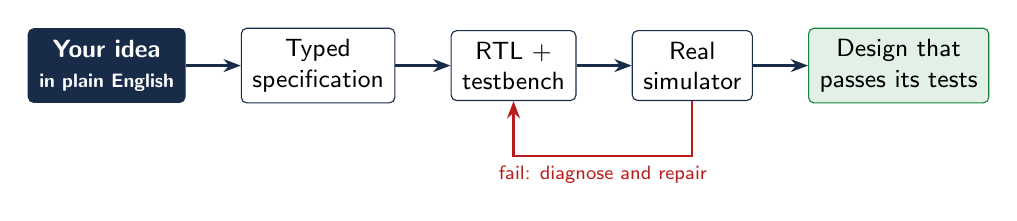
\begin{tikzpicture}[node distance=7mm]
  \node[hbox] (p) {Your idea\\ \scriptsize in plain English};
  \node[box,right=of p] (s) {Typed\\ specification};
  \node[box,right=of s] (g) {RTL +\\ testbench};
  \node[box,right=of g] (sim) {Real\\ simulator};
  \node[okbox,right=of sim] (ok) {Design that\\ passes its tests};
  \draw[arr] (p)--(s); \draw[arr] (s)--(g); \draw[arr] (g)--(sim); \draw[arr] (sim)--(ok);
  \draw[arr,badred] (sim.south) -- ++(0,-0.7) -| node[pos=0.25,below,font=\scriptsize,text=badred]{fail: diagnose and repair} (g.south);
\end{tikzpicture}

\vfill
{\large Written for readers with \textbf{no previous knowledge} of chip design, Verilog, AI or web development}\\[1.2cm]
{\large\bfseries Kushal Pitaliya \quad(Roll No.\ 23EC105)}\\[4pt]
EC486 Minor Project \textbullet\ B.Tech Electronics \& Communication Engineering, 7th Semester\\[2pt]
V.\ T.\ Patel Department of Electronics \& Communication Engineering, CSPIT, CHARUSAT\\[2pt]
Academic Year 2026--27 \textbullet\ November 2026
\end{titlepage}

\pagenumbering{roman}
\tableofcontents
\clearpage

% ============================================================== HOW TO READ ==
\chapter*{How to Use This Guide}
\addcontentsline{toc}{chapter}{How to Use This Guide}
\markboth{How to Use This Guide}{}

This manual explains SiliconScribe from the ground up. It assumes you know nothing about digital hardware, Verilog, artificial intelligence or web software. Every technical word is explained the first time it appears, and the Glossary (Appendix~\ref{app:glossary}) collects them all.

\begin{center}
\begin{tabularx}{\textwidth}{@{}>{\bfseries}p{4.1cm}X@{}}
\toprule
If you are\ldots & Read\ldots \\
\midrule
Completely new & Part~I in order (Chapters 1--7), then Chapter~\ref{ch:journey} (the journey of one request). \\
A student preparing for the viva & Chapters~\ref{ch:bigpicture}, \ref{ch:journey}, \ref{ch:pipeline} and \ref{ch:why}, then the question bank in Chapter~\ref{ch:vivaqa}. \\
A developer who wants to run or change the code & Part~II (Chapters~\ref{ch:arch}--\ref{ch:agent}) and Part~III, with the function index in Appendix~\ref{app:index}. \\
An examiner checking the claims & Chapters~\ref{ch:pipeline}, \ref{ch:trust}, \ref{ch:timing}, \ref{ch:simulator}, \ref{ch:testing} and \ref{ch:why}. \\
\bottomrule
\end{tabularx}
\end{center}

Throughout the guide you will see four kinds of boxes:

\begin{keyidea}
The single most important point of a section. If you read nothing else, read these.
\end{keyidea}
\begin{analogy}
A comparison with everyday life, to build intuition before the technical detail.
\end{analogy}
\begin{viva}
A question an examiner is likely to ask, and how to answer it in your own words.
\end{viva}
\begin{warnbox}
A limitation, a common mistake, or something the system deliberately does \emph{not} do.
\end{warnbox}

File names such as \file{backend/orchestrator.py} and function names such as \code{pipeline_events} refer to the real code in the project folder \file{ai-eda-playground/}. Everything described here was checked against that code; nothing is invented or assumed.

\clearpage
\pagenumbering{arabic}

% ============================================================== PART I =====
\part{Background from Zero}
% ============================================================================
%  PART I: Background from zero
% ============================================================================

\chapter{The Big Picture in One Chapter}
\label{ch:bigpicture}

\section{What SiliconScribe is}

SiliconScribe is a web application. You type a description of a small piece of digital hardware in plain English, for example:

\begin{quote}\itshape
``Design a 4-bit synchronous up-counter with async reset and enable.''
\end{quote}

and after a while (a short wait with the built-in offline designs; with a free live AI model, a few minutes: the median in the evaluation was 360 seconds) you get back:

\begin{enumerate}
  \item \textbf{RTL code}: the hardware described in the Verilog language, ready for a chip or FPGA flow.
  \item \textbf{A testbench}: a second Verilog program whose only job is to test the first one.
  \item \textbf{A verdict from a real simulator}: PASS or FAIL, with how many checks passed and failed, and every check listed.
  \item \textbf{A waveform}: a picture of every signal changing over time.
  \item \textbf{If something failed}: a diagnosis of why, a minimal fix, and the evidence that the fix worked.
  \item \textbf{How much the PASS is worth}: how many deliberately injected bugs the testbench catches, how much of the design's wiring the test actually exercised, and (after some repairs) a second opinion from a fresh testbench.
  \item \textbf{An early size and speed estimate}: the design mapped onto real chip cells (SkyWater 130 nm), with its area and whether it meets the target clock. This is a pre-layout estimate, not a final chip measurement.
\end{enumerate}

The words ``RTL'', ``Verilog'', ``testbench'' and ``simulator'' are all explained in the next chapters. For now, the important point is the idea behind the project.

\section{The problem it solves}

Large language models (LLMs) such as the ones behind ChatGPT can write Verilog. But they write it the way a student writes an exam answer without ever checking it: they never run the code. The model produces text that \emph{looks} right. Whether the hardware actually works is a different question, and the model cannot answer it.

When people use a chat model directly for hardware, three things go wrong (Chapter~\ref{ch:ai} explains each one):

\begin{enumerate}
  \item The code often does not compile with real tools.
  \item The model cannot observe its own design running, so it cannot know whether it is correct.
  \item When told ``make it pass'', models tend to weaken or delete the tests instead of fixing the design.
\end{enumerate}

\section{The core idea: close the loop with a real simulator}

\begin{keyidea}
SiliconScribe never trusts the AI's claim that a design works. A real Verilog simulator (Icarus Verilog) runs every design, and only the simulator's result decides PASS or FAIL. The AI writes; the simulator judges.
\end{keyidea}

\begin{figure}[H]
\centering
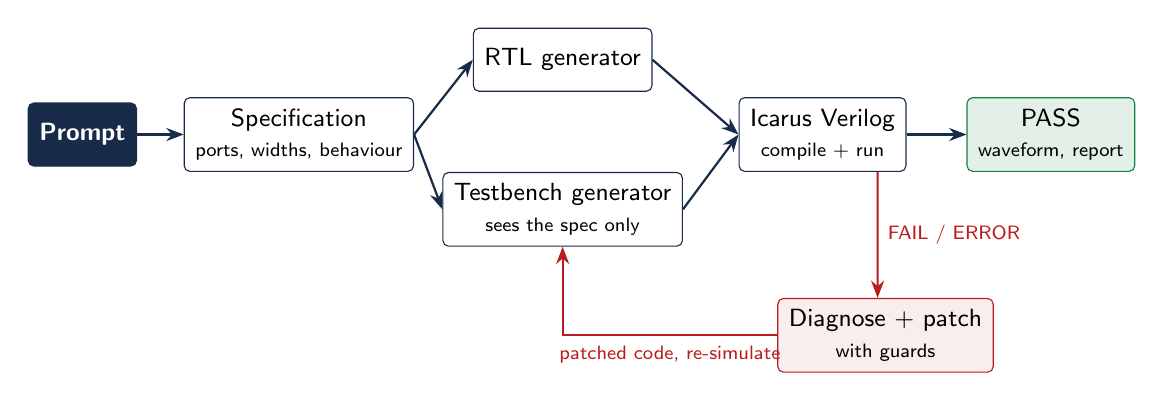
\begin{tikzpicture}
  \node[hbox] (p) at (0,0) {Prompt};
  \node[box] (spec) at (2.75,0) {Specification\\ \scriptsize ports, widths, behaviour};
  \node[box] (rtl) at (6.1,0.95) {RTL generator};
  \node[box] (tb) at (6.1,-0.95) {Testbench generator\\ \scriptsize sees the spec only};
  \node[box] (sim) at (9.4,0) {Icarus Verilog\\ \scriptsize compile + run};
  \node[okbox] (pass) at (12.3,0) {PASS\\ \scriptsize waveform, report};
  \node[badbox] (fix) at (10.2,-2.55) {Diagnose + patch\\ \scriptsize with guards};
  \draw[arr] (p)--(spec); \draw[arr] (spec.east)--(rtl.west); \draw[arr] (spec.east)--(tb.west);
  \draw[arr] (rtl.east)--(sim.west); \draw[arr] (tb.east)--(sim.west); \draw[arr] (sim)--(pass);
  \draw[arr,badred] ($(sim.south)+(0.7,0)$) -- node[right,font=\scriptsize]{FAIL / ERROR} ($(fix.north)+(-0.1,0)$);
  \draw[arr,badred] (fix.west) -- (tb.south |- fix.west) node[midway,below,font=\scriptsize]{patched code, re-simulate} -- (tb.south);
\end{tikzpicture}
\caption{The closed loop. Two generators work from the same specification but never see each other's code; the simulator is the only judge.}
\label{fig:loop}
\end{figure}

\begin{analogy}
Think of an exam. If the same student writes both the answers and the answer key, a wrong answer and a wrong key can agree, and the student ``scores'' full marks. SiliconScribe has the answer key (the testbench) written from the \emph{question} (the specification), never from the student's answer (the RTL). Then an impartial examiner (the simulator) marks the paper.
\end{analogy}

\section{What makes it trustworthy}

These safeguards stop the system from fooling itself or its user:

\begin{description}
  \item[Independent testbench.] The testbench generator is never shown the RTL. It derives every expected value from the specification. Optionally a \emph{different} AI model writes it.
  \item[Simulator as the oracle.] PASS or FAIL comes from the simulator output, never from the model. A PASS needs a valid summary and at least one executed check.
  \item[Anti-cheat guard.] A ``fix'' that deletes test checks from a testbench that already ran is rejected. If a repair changed the testbench, the original one is run again and a fresh second-opinion testbench is asked for.
  \item[Loop guards.] If a fix changes nothing, or brings back a version already tried, the loop stops instead of burning time.
  \item[Testing the test.] After every PASS, small bugs are injected into the design to see whether the testbench notices (testbench strength), and toggle coverage is measured from the simulator's own waveform file.
  \item[You can check the question.] The specification the model wrote can be reviewed and edited before anything is built.
  \item[Honest degraded mode.] If the AI service is unavailable, the app says so clearly and labels results as coming from built-in examples. A model you chose yourself is never silently replaced.
\end{description}

\section{Results in numbers}

\begin{center}
\begin{tabular}{@{}lr@{}}
\toprule
Live evaluation, 15 prompts (DeepSeek V4.1 Flash) & 14 done: 8 PASS at once, 6 after repair \\
Median time per live run & 360 s (3 to 13 minutes) \\
Injected bugs caught by the live testbenches & 102 of 111 (92\%) \\
Evaluated designs correct against hand-written references & 14 of 14 \\
Mutation sweep of the built-in designs & 27 of 27 caught \\
Timing netlists equal to the RTL at gate level & 19 of 19 designs \\
Automated tests & 436 backend + 211 frontend, all passing \\
\bottomrule
\end{tabular}
\end{center}

The 15th prompt (a 4-bit counter) did not complete: testbench generation timed out three times. It is reported as ``no result'', never as a pass or a failure. Chapter~\ref{ch:testing} lists the commands behind every number.

% ---------------------------------------------------------------------------
\chapter{Digital Hardware Basics}
\label{ch:hardware}

This chapter gives just enough electronics to understand what the generated designs do.

\section{Bits, signals and buses}

Digital hardware works with \textbf{bits}: values that are either 0 or 1 (in a real circuit, a low or a high voltage). A wire carrying one bit is a \textbf{signal}. A group of wires that together carry a number is a \textbf{bus}, and the number of wires is its \textbf{width}. A 4-bit bus can carry the numbers 0 to 15 ($2^4-1$); an 8-bit bus carries 0 to 255.

Bus values are usually written in \textbf{hexadecimal} (base 16, digits 0--9 and a--f), so the 4-bit value 1011 (eleven) is written \code{b} and the 8-bit value 1111 1111 is \code{ff}. SiliconScribe's waveform viewer shows buses this way.

\section{Logic gates and combinational logic}

A \textbf{logic gate} computes an output bit from input bits: AND (1 only if all inputs are 1), OR (1 if any input is 1), NOT (inverts), XOR (1 if the inputs differ). Connecting gates gives \textbf{combinational logic}: circuits whose outputs depend \emph{only} on the current inputs, with no memory. Examples SiliconScribe can build:

\begin{itemize}
  \item \textbf{Multiplexer (mux)}: a selector. A 4:1 mux has four data inputs and a 2-bit select input; the output copies whichever input is selected.
  \item \textbf{Full adder}: adds two bits and a carry-in, producing a sum bit and a carry-out.
  \item \textbf{Priority encoder}: given 8 request lines, outputs the index (0--7) of the highest-numbered active line, plus a ``valid'' flag that is 1 if any line is active.
  \item \textbf{ALU} (arithmetic logic unit): computes add, subtract, AND, OR, XOR and so on, chosen by an \textbf{opcode} input, and flags conditions such as overflow.
\end{itemize}

\section{Sequential logic, clocks and resets}

\textbf{Sequential logic} has memory: its outputs depend on the past as well as the present. The memory elements are \textbf{flip-flops} (one bit each); a group of flip-flops holding a value is a \textbf{register}.

Flip-flops change only at the instant a \textbf{clock} signal rises from 0 to 1 (the \textbf{rising edge} or \code{posedge}). The clock is a square wave that ticks millions of times per second; its frequency (for example 100 MHz) is the ``target frequency'' you can set in the app.

A \textbf{reset} forces registers to a known starting value. Two properties matter:

\begin{itemize}
  \item \textbf{Synchronous vs asynchronous}: a synchronous reset takes effect at the next clock edge; an asynchronous reset takes effect immediately.
  \item \textbf{Active-high vs active-low}: an active-low reset (often named \code{rst_n}, ``n'' for negative) resets when the signal is 0.
\end{itemize}

\begin{analogy}
A clock is like a drummer in a marching band: nobody moves between beats, and on each beat everyone takes exactly one step. A reset is the band leader shouting ``back to the start line''.
\end{analogy}

The \textbf{counter} used throughout this guide is sequential: on every rising clock edge, if \code{enable} is 1, its 4-bit \code{count} goes up by one (wrapping from 15 back to 0); if \code{enable} is 0 it holds its value; and an active-low asynchronous reset clears it to 0 at once.

\section{RTL: the level designers work at}

Engineers do not draw millions of gates. They describe hardware at the \textbf{register-transfer level (RTL)}: which registers exist and how values move between them on each clock edge. A tool called a \textbf{synthesizer} later converts RTL into gates. ``Generating RTL'' therefore means writing the design description, not drawing the circuit.

% ---------------------------------------------------------------------------
\chapter{Describing Hardware with Verilog}
\label{ch:verilog}

\textbf{Verilog} is a hardware description language (HDL). It looks a little like the C programming language, but it describes circuits that all run at the same time, not instructions that run one after another. \textbf{SystemVerilog} is its modern superset. SiliconScribe generates Verilog-2001 style code because the simulator it uses (Icarus Verilog) supports that best.

\section{A complete example: the curated counter}

This is the real counter design that ships with SiliconScribe (\file{backend/offline_designs.py}):

\begin{lstlisting}
module counter #(
    parameter WIDTH = 4
)(
    input  wire             clk,
    input  wire             rst_n,
    input  wire             enable,
    output reg  [WIDTH-1:0] count
);
    always @(posedge clk or negedge rst_n) begin
        if (!rst_n)
            count <= {WIDTH{1'b0}};
        else if (enable)
            count <= count + 1'b1;
    end
endmodule
\end{lstlisting}

Line by line:

\begin{description}[style=nextline]
  \item[\code{module counter ... endmodule}] A \textbf{module} is one hardware block, like a chip with pins. Everything between \code{module} and \code{endmodule} describes it.
  \item[\code{parameter WIDTH = 4}] A \textbf{parameter} is a constant that can be changed when the module is used, so the same code can build a 4-bit or 8-bit counter.
  \item[\code{input wire clk}] The \textbf{ports} are the pins. \code{input} and \code{output} give the direction. \code{[WIDTH-1:0]} declares a bus from bit 3 down to bit 0.
  \item[\code{wire} vs \code{reg}] A \code{wire} is a plain connection driven continuously. A \code{reg} is a variable assigned inside an \code{always} or \code{initial} block. Mixing them up is one of the most common errors, and SiliconScribe repairs it automatically (Section~\ref{sec:compilerrepair}).
  \item[\code{always @(posedge clk or negedge rst_n)}] Run this block on every rising clock edge, or the moment reset falls to 0 (that is what makes the reset asynchronous).
  \item[\code{if (!rst_n) count <= ...}] If reset is active (0), clear the count. \texttt{\{WIDTH\{1'b0\}\}} means ``WIDTH copies of a single 0 bit''.
  \item[\code{count <= count + 1'b1}] Otherwise, if enabled, add one. The \code{<=} is a \textbf{non-blocking assignment}: all registers update together at the clock edge, exactly like real flip-flops.
\end{description}

\section{Number literals}

Verilog numbers carry their width and base: \code{1'b1} is a 1-bit binary 1, \code{2'd2} is a 2-bit decimal 2, \code{4'hF} is a 4-bit hexadecimal 15, and \code{8'b1???????} uses \code{?} as ``don't care'' bits inside a \code{casez} statement. This matters later: the seeded bug in the live repair demo was \code{count + 2'd2} (count by two) instead of \code{count + 1'b1}.

\section{Four-valued logic: 0, 1, x and z}

A simulated signal can be 0, 1, \code{x} (unknown, for example an uninitialised register) or \code{z} (high impedance, an undriven wire). This is why testbenches compare with \code{===} (case equality, which treats \code{x} as a distinct value) rather than \code{==} (which returns unknown if either side contains \code{x}). With \code{==}, an output stuck at \code{x} could slip past a check; with \code{===} it fails.

\section{Combinational code and casez}

Combinational logic is written with \code{assign} (continuous assignment) or an \code{always @(*)} block. The live-generated priority encoder used a \code{casez} statement, which matches patterns with don't-care bits, highest priority first:

\begin{lstlisting}
always @(*) begin
    code = 3'd0; valid = 1'b0;
    casez (in)
        8'b1???????: begin code = 3'd7; valid = 1'b1; end
        8'b01??????: begin code = 3'd6; valid = 1'b1; end
        // ... down to ...
        8'b00000001: begin code = 3'd0; valid = 1'b1; end
        default:     begin code = 3'd0; valid = 1'b0; end
    endcase
end
\end{lstlisting}

\section{Constructs Icarus Verilog rejects}

Icarus Verilog 12.0 in its \code{-g2012} mode accepts much of the synthesizable SystemVerilog that LLMs write: \code{logic}, \code{always_ff}, \code{always_comb}, \code{enum}, packed structs, \code{return} inside functions, \code{string} and queues, and simple classes and immediate \code{assert} statements. It rejects a specific set: \code{break} and \code{continue}; \code{disable} of a function (the error is ``Cannot disable functions'', although \code{disable} of a named block or a task is fine); the \code{inside} operator; streaming concatenation; concurrent assertions (\code{property}, \code{sequence}); virtual classes and class \code{constraint} blocks; and interface \code{modport}s. Each of these was checked by compiling a one-line example. The generation prompts therefore ask for conservative Verilog-2001 style, which avoids the whole list and stays portable to other tools, and the orchestrator repairs the two most common failures automatically when they still appear.

% ---------------------------------------------------------------------------
\chapter{Verification: Proving a Design Works}
\label{ch:verification}

\section{DUT and testbench}

The design being tested is the \textbf{DUT} (device under test). A \textbf{testbench} is a separate Verilog module, conventionally named \code{testbench}, that has no ports of its own. It creates the DUT inside itself, drives its inputs (the \textbf{stimulus}), watches its outputs, and checks them against \textbf{expected values}. The thing that knows the expected values is called the \textbf{oracle} or \textbf{reference model}.

A \textbf{self-checking} testbench does the comparison itself and prints a verdict, so no human has to read waveforms to decide whether the design works.

\section{The curated counter testbench, explained}

The listing is a simplified teaching version of the idea. The shipped testbench has the same structure, but it logs every comparison through a small \code{chk} task (so the Test cases tab can list each check with its type) and runs 57 checks of four types: reset, directed, hold and corner.

\begin{lstlisting}
`timescale 1ns/1ps
module testbench;
    reg clk, rst_n, enable;
    wire [3:0] count;
    integer pass_count = 0;
    integer fail_count = 0;
    integer expected;

    counter #(4) dut (.clk(clk), .rst_n(rst_n), .enable(enable), .count(count));

    initial clk = 0;
    always #5 clk = ~clk;            // a clock with a 10 ns period

    initial begin
        rst_n = 0; enable = 0; expected = 0;
        @(negedge clk); rst_n = 1; enable = 1;
        repeat (20) begin
            @(negedge clk);
            expected = (expected + 1) % 16;   // the oracle
            if (count === expected[3:0]) pass_count = pass_count + 1;
            else begin
                $display("FAIL: expected=%0d got=%0d", expected, count);
                fail_count = fail_count + 1;
            end
        end
        // ... phases 2-4: enable low must HOLD, async reset must CLEAR,
        //     counting must RESUME from zero (more checks in the shipped file) ...
        $display("Passed: %0d", pass_count);
        $display("Failed: %0d", fail_count);
        if (fail_count == 0) $display("ALL TESTS PASSED");
        $finish;
    end
endmodule
\end{lstlisting}

\begin{itemize}
  \item \code{`timescale 1ns/1ps} sets the unit of delays: \texttt{\#5} means 5 ns.
  \item \texttt{counter \#(4) dut (...)} \textbf{instantiates} the DUT and connects its ports to the testbench's signals.
  \item \texttt{always \#5 clk = \textasciitilde clk} toggles the clock every 5 ns.
  \item \code{@(negedge clk)} waits for the falling clock edge, so checks happen safely between rising edges.
  \item \code{$display} prints to the simulator transcript; \code{$finish} ends the simulation.
  \item The three final lines are a \textbf{contract} with SiliconScribe: the simulator wrapper reads \code{Passed:}, \code{Failed:} and \code{ALL TESTS PASSED} from the transcript to decide the verdict (Section~\ref{sec:verdict}).
\end{itemize}

\section{Directed and random stimulus}

\textbf{Directed} tests are hand-picked cases, usually corner cases such as all zeros, all ones, and each single active bit. \textbf{Random} tests use \code{$random} to try many arbitrary inputs. SiliconScribe's testbench prompt asks for both: directed corner cases plus at least 100 randomized vectors.

\begin{warnbox}
Random testing is strong but not exhaustive. The archived priority-encoder testbench uses 16 directed cases and 100 random vectors, so it checks many but not all of the 256 possible 8-bit inputs. That is honest evidence, not proof.
\end{warnbox}

\section{Coverage}

\textbf{Coverage} measures how much of the design or its behaviour the tests exercised. Industrial flows use instrumented code coverage (lines, branches, toggles) and functional coverage (which interesting cases occurred). SiliconScribe measures one of these itself: \textbf{toggle coverage}, the share of the design's signal bits that the simulation saw go both from 0 to 1 and from 1 to 0. A bit that never moved was never really tested. It is read from the simulator's own waveform file, not from what the testbench claims (Section~\ref{sec:toggle}). Line and branch coverage are not measured.

\section{Mutation testing: testing the tests}
\label{sec:mutation}

How do you know a testbench is good? Break the design on purpose and see whether the testbench notices. Each deliberately broken copy is a \textbf{mutant}; if the testbench fails it, the mutant is \textbf{killed}; if it still passes, the mutant \textbf{survived} and the testbench has a blind spot. This idea, called \textbf{mutation testing}, comes from DeMillo, Lipton and Sayward (1978).

SiliconScribe uses the idea twice. First, a fixed sweep (\file{backend/tools/mutation_sweep.py}) injects known bugs such as ``count by two'', ``reset ignored'', ``enable ignored'', ``ADD replaced by SUB'' and ``mux inputs swapped'' into the built-in designs. An early 14-bug version caught only 11; the three survivors exposed real gaps (enable not tested, overflow flag not checked, undefined opcodes not driven). After the testbenches were hardened and the sweep grew to 27 bugs, all 27 are caught. Second, and more important, the app does it automatically after every PASS, on the model's own design and testbench: this is the \textbf{testbench strength} shown with each result (Section~\ref{sec:strength}).

One caution: a mutant can be \textbf{equivalent}, meaning the change does not alter what the design does (for example in code that can never be reached). No testbench can catch it, so a survivor is ``not noticed'', not ``proven missed''.

\section{Why the oracle must be independent}

\begin{keyidea}
If the same model, looking at the same RTL, writes the testbench, it tends to encode the same mistake in both, and a wrong design passes. SiliconScribe withholds the RTL from the testbench generator so the expected values must come from the specification.
\end{keyidea}

\begin{warnbox}
One common-mode risk remains: by default the \emph{same} model reads the \emph{same} specification for both. If it misreads the spec, both can be wrong in the same way. SiliconScribe offers three answers: you can review and correct the specification before generation; you can choose a \emph{different} model to write the testbench; and after a repair that rewrote the testbench, a fresh testbench gives a second opinion (Chapter~\ref{ch:trust}). For the evaluation, hand-written reference testbenches were used as an outside check.
\end{warnbox}

% ---------------------------------------------------------------------------
\chapter{EDA Tools Used}
\label{ch:tools}

\textbf{EDA} (electronic design automation) is the software chip engineers use. SiliconScribe drives these tools as separate programs (subprocesses).

\section{Icarus Verilog: the simulator}

\textbf{Icarus Verilog} is a free, open-source Verilog simulator. It works in two steps:

\begin{enumerate}
  \item \textbf{Compile} with \code{iverilog}: read the source files, check them, and produce a compiled simulation file (\file{testbench.vvp}). Syntax or type errors stop here; SiliconScribe reports this as status \textbf{ERROR}.
  \item \textbf{Run} with \code{vvp}: execute the compiled simulation. The testbench's \code{$display} output goes to a transcript (\file{transcript.log}); signal changes go to a waveform file.
\end{enumerate}

SiliconScribe uses exactly this command to compile:
\begin{lstlisting}[style=plain]
iverilog -o testbench.vvp -g2012 -Wall _timescale.v design.sv testbench.sv
\end{lstlisting}
where \code{-g2012} enables the 2012 language mode and \code{-Wall} turns on all warnings. \file{_timescale.v} is a one-line file the app writes (\code{`timescale 1ns/1ps}) so every file gets a sensible default time unit.

\section{VCD: the waveform file}

A \textbf{VCD} (value change dump) file is a plain-text record of every signal change. The testbench requests one with \code{$dumpfile("design.vcd")} and \code{$dumpvars}. If a generated testbench forgets, SiliconScribe adds those lines automatically. A small excerpt looks like:

\begin{lstlisting}[style=plain]
$var wire 1 ! clk $end
$var reg 4 " count [3:0] $end
$enddefinitions $end
#0
0!
b0000 "
#5
1!
b0001 "
\end{lstlisting}

Each signal gets a short code (\code{!}, \code{"}); \texttt{\#5} means ``time 5''; \code{1!} means ``clk became 1''; \code{b0001 "} means ``count became binary 0001''. SiliconScribe's own parser turns this into data the browser draws (Section~\ref{sec:vcd}).

\section{Yosys: synthesis}

\textbf{Yosys} is an open-source synthesizer: it converts RTL into a \textbf{netlist} of gates and reports how many cells (gates and flip-flops) the design needs. SiliconScribe uses it twice:
\begin{itemize}
  \item \textbf{Generic synthesis}, without a cell library: a count of Yosys' own generic cells, flip-flops and latches. Its area figure is only a \emph{relative proxy} (cells $\times$ 5), not square micrometres, and the app labels it so.
  \item \textbf{Mapping to real cells} for the timing and area estimate: the design is mapped onto the cells of a real chip library (next section), which gives a real area in square micrometres (\umsq{}).
\end{itemize}
SiliconScribe uses Yosys 0.71 as a WebAssembly build (\code{yowasp-yosys}), so it installs with pip. If Yosys is missing, the app says ``Synthesis not available'' instead of inventing numbers.

\section{Cell libraries, sky130 and OpenSTA: timing}

A real chip is built from a foundry's library of small pre-designed blocks called \textbf{standard cells} (NAND gates, inverters, flip-flops\ldots). For each cell, a \textbf{liberty file} gives its area and how long a signal takes to pass through it. SiliconScribe uses the open \textbf{SkyWater 130 nm} library (\textbf{sky130}), at its typical operating point (25\,\textdegree C, 1.8 V).

\textbf{OpenSTA} is an open-source \textbf{static timing analysis} tool. Instead of simulating, it adds up the cell delays along every path between flip-flops (or from inputs to outputs) and compares the slowest one with the clock period. The time left over is the \textbf{slack}: positive means the design is fast enough for the target clock, negative means it is too slow.

\begin{warnbox}
These numbers are a \textbf{pre-layout estimate}: the cells are not yet placed on a chip, so the delay of the wires between them is not included, the clock is ideal, and only one operating point is checked. They answer ``is this anywhere near the target clock, and roughly how big is it?''. They are not the final timing checks done before a chip is made, and not the area of a manufactured chip. Chapter~\ref{ch:timing} explains the details.
\end{warnbox}

\section{Verilator: linting}

\textbf{Linting} means checking code for suspicious patterns without running it. SiliconScribe's linter uses Verilator if available, otherwise Icarus, otherwise simple built-in pattern checks. Lint results are shown for information only and never block the pipeline.

\section{UVM: the industrial testbench style}

\textbf{UVM} (Universal Verification Methodology) is the industry-standard way to build large testbenches in SystemVerilog classes: a sequencer generates transactions, a driver applies them, a monitor observes, a scoreboard checks, and coverage is collected. SiliconScribe can \emph{export} a 16-file UVM bundle for a commercial simulator. It cannot run it, because Icarus does not support UVM, and no commercial licence was available. The export is labelled accordingly.

% ---------------------------------------------------------------------------
\chapter{AI Basics: Language Models and APIs}
\label{ch:ai}

\section{What a large language model is}

A \textbf{large language model (LLM)} is a program trained on huge amounts of text to predict the next piece of text. Given a \textbf{prompt}, it writes a continuation one \textbf{token} (a word fragment) at a time. Because it has read a great deal of code, it can write plausible Verilog. But it predicts text; it does not run circuits.

\section{The words you will meet}

\begin{description}
  \item[System prompt.] Standing instructions sent before the user's message (``You are an expert Verilog designer\ldots''). SiliconScribe has one per stage; Appendix~B of the project report prints them in full.
  \item[Temperature.] How random the output is. Low (0.2) gives focused, repeatable answers; SiliconScribe uses 0.2 for RTL and fixes, 0.3 for the specification and testbench, 0.5 for the explanation.
  \item[Max tokens.] The maximum length of an answer (8192 by default here, configurable with \code{LLM_MAX_TOKENS}).
  \item[Reasoning tokens.] Some models ``think'' in hidden tokens before answering. Those count against max tokens, so a model can use its whole budget thinking and return nothing. SiliconScribe disables hidden reasoning unless the user asks for it.
  \item[API.] An application programming interface: a way for one program to call another over the internet. LLMs are reached through an HTTP API.
  \item[OpenAI-compatible API.] Many providers (Cloudflare Workers AI, NVIDIA NIM, OpenRouter, OpenCode Zen, local servers) accept the same request format as OpenAI. SiliconScribe uses one client for all of them.
  \item[The OpenCode app.] A coding-assistant program you install and sign in to with your own account. It offers several hundred models, some free. SiliconScribe can use it as its model source by running the app's own command-line interface (Section~\ref{sec:routing}). GitHub Copilot can be connected inside the OpenCode app and then appears there too.
  \item[API key.] A secret string that proves to a provider who is calling. In SiliconScribe keys live only in the file \file{backend/.env} on your own computer; the web page never asks for one.
  \item[Hallucination.] When a model confidently states something false. SiliconScribe's answer is to never take the model's word for correctness.
\end{description}

\section{Why an LLM alone fails at hardware}

\begin{enumerate}
  \item \textbf{Toolchain incompatibility.} Models emit SystemVerilog features Icarus rejects, so the code never compiles.
  \item \textbf{No execution awareness.} A model cannot see a clock edge, a race condition or a failing check. It can only produce text that resembles working code.
  \item \textbf{No real diagnosis.} Asked to ``make it pass'', a model often weakens the testbench, deletes checks or swaps in a different design. That is test evasion, not debugging.
\end{enumerate}

Each failure has a direct answer in SiliconScribe: Icarus-safe prompts plus automatic compiler repairs; the simulator as the judge; and the anti-cheat and loop guards.

\section{Free tiers and model quality}

The project was built on a zero budget, so live runs used free models. The report documents a measured case: a small free model produced plausible but wrong logic for the priority encoder, while a larger free model produced a correct design that passed first time. Same pipeline, same simulator; only the model differed. Quality therefore rises with the model, and the architecture does not need to change. That is why the model can be chosen per run from a menu.

Free models have costs of their own: they are slow (the final evaluation with DeepSeek V4.1 Flash took a median of 360 seconds per run, up to 13 minutes), their daily quotas run out, and their names change or disappear. One free model on Cloudflare wrote a correct counter but a testbench whose watchdog timer was shorter than its own test, so it never printed a summary; the app reported ERROR with 0 checks instead of calling it a PASS.

% ---------------------------------------------------------------------------
\chapter{Web Software Basics}
\label{ch:web}

\section{Frontend and backend}

A web application has two halves:

\begin{itemize}
  \item The \textbf{frontend} runs in your browser and draws the interface. SiliconScribe's is written in \textbf{TypeScript} (JavaScript with types) using \textbf{React}, a library that builds the page from reusable \textbf{components} and redraws them when their \textbf{state} (data) changes. \textbf{Vite} is the tool that builds and serves it during development.
  \item The \textbf{backend} runs on a server and does the work. SiliconScribe's is written in \textbf{Python} using \textbf{FastAPI}, a framework that turns Python functions into web addresses (\textbf{endpoints}).
\end{itemize}

\begin{analogy}
The frontend is a restaurant's dining room and menu; the backend is the kitchen. You order at the table (click Generate), the waiter carries the order (an HTTP request), and the kitchen cooks (generates and simulates) and sends the dish back.
\end{analogy}

\section{HTTP, JSON and endpoints}

The browser and server talk using \textbf{HTTP}. A request has a method (\code{GET} to read, \code{POST} to send data, \code{DELETE} to remove) and a path such as \code{/api/design/stream}. Data travels as \textbf{JSON}, a text format of named fields, for example \texttt{\{"prompt": "Design a counter", "max\_iterations": 5\}}. The server answers with a status code: 200 means OK, 422 means invalid input, 429 means too many requests, 500 means a server error.

\section{Streaming with Server-Sent Events}

A full generation takes from seconds (offline) to several minutes (free live models). Instead of making you wait for one big answer, the backend sends a series of small messages as each stage finishes, using \textbf{Server-Sent Events (SSE)}: one long HTTP response in which each message is a line starting with \code{data:} followed by JSON, and messages are separated by a blank line. The frontend reads them as they arrive and updates the agent timeline live.

\section{Data validation with Pydantic}

\textbf{Pydantic} lets the backend declare the exact shape of every piece of data (for example: a prompt is text of at most 2000 characters; a port width is an integer from 1 to 1024). Invalid requests are rejected automatically with HTTP 422 before any work starts. The shapes live in \file{backend/models.py}.

\section{Storage with SQLite}

\textbf{SQLite} is a small database stored in one file. SiliconScribe keeps every finished run in \file{backend/workspace/projects.db} so the Projects menu can list and reload them.

\section{Threads and blocking}

A web server handles many requests at once. FastAPI can run a handler either on its main \textbf{event loop} (\code{async def}) or in a pool of \textbf{threads} (plain \code{def}). Work that waits on a subprocess, such as a simulation, must not run on the event loop, or every other request freezes until it finishes. The final review found exactly that bug (a health check took 6.5 seconds during an 8-second simulation) and fixed it by making those handlers plain \code{def}; the health check now answers in about 1 ms.

\section{Safety basics: CORS and rate limiting}

\textbf{CORS} (cross-origin resource sharing) tells browsers which websites may call the API; SiliconScribe allows pages from this machine only (\code{localhost} and \code{127.0.0.1}), and any other address must be added by name with \code{CORS_ALLOW_ORIGINS}. This matters because the backend holds model keys: a stranger's web page must not be able to make your browser use them. \textbf{Rate limiting} stops one user from flooding the server: at most 20 requests per minute per IP address, otherwise HTTP 429.


\part{How SiliconScribe Works}
% ============================================================================
%  PART II: How SiliconScribe works
% ============================================================================

\chapter{Architecture and Code Map}
\label{ch:arch}

\section{Three tiers}

\begin{figure}[H]
\centering
\begin{tikzpicture}[node distance=10mm and 8mm]
  \node[hbox,minimum width=13.4cm] (fe) {FRONTEND \quad React 18 + Vite + TypeScript (runs in the browser)};
  \node[box,below=3mm of fe.south west,anchor=north west,minimum width=13.4cm,align=left,font=\scriptsize] (fed)
    {Sidebar: prompt, run timeline, examples, Model menu, ``Testbench written by'', specification review, target clock \\
     ``Ask about this run'' (the debugging agent) under the run timeline \\
     Design / Results / Test cases / Waveform / Schematic tabs \textbullet\ Projects menu \textbullet\ Export UVM, Re-run, Stop \textbullet\ theme};
  \node[hbox,below=12mm of fed.south west,anchor=north west,minimum width=9.1cm] (be) {BACKEND \quad FastAPI + Pydantic (Python)};
  \node[box,below=3mm of be.south west,anchor=north west,minimum width=9.1cm,text width=8.8cm,align=left,font=\scriptsize] (bed)
    {\file{main.py}: routes, CORS, rate limit, SSE streaming\\
     \file{orchestrator.py}: pipeline, repair loop, second opinion\\
     \file{llm_service.py} + \file{model_catalog.py}: providers, model menu, prompts\\
     \file{simulator.py}: Icarus Verilog and sandbox\\
     \file{mutation.py}: testbench strength \textbullet\ \file{timing.py}: timing and area\\
     \file{equivalence.py}: proof that the netlist equals the RTL\\
     \file{agent.py} + \file{wave_query.py}: the debugging agent\\
     linter, checks, VCD parser and toggle coverage, schematic, synthesis, UVM export, SQLite};
  \node[hbox,right=4mm of be,minimum width=3.9cm] (llm) {LLM PROVIDERS};
  \node[box,below=3mm of llm.south west,anchor=north west,minimum width=3.9cm,text width=3.6cm,align=left,font=\scriptsize] (llmd)
    {OpenCode app (local)\\ Cloudflare Workers AI\\ NVIDIA NIM\\ any OpenAI-compatible API\\ keys only in \file{backend/.env}};
  \node[hbox,below=12mm of bed.south west,anchor=north west,minimum width=9.1cm] (eda) {EDA TOOLCHAIN \quad local subprocesses};
  \node[box,below=3mm of eda.south west,anchor=north west,minimum width=9.1cm,align=left,font=\scriptsize] (edad)
    {Icarus Verilog 12 (\code{iverilog}, \code{vvp}) \textbullet\ Yosys 0.71 \textbullet\ OpenSTA 3.2.0 \textbullet\ sky130 cell library\\ Verilator if installed \textbullet\ one workspace folder per design, time limits, scrubbed environment};
  \draw[arr,<->] (fed.south) ++(-2.5,0) -- node[right,font=\scriptsize]{HTTP + Server-Sent Events} ++(0,-1.2);
  \draw[arr,<->] (bed.east) -- (llmd.west);
  \draw[arr] (bed.south) ++(-1,0) -- node[right,font=\scriptsize]{subprocess} ++(0,-1.2);
\end{tikzpicture}
\caption{The three tiers. The backend is the only part that holds secrets or runs programs.}
\end{figure}

\begin{keyidea}
The browser never talks to the AI provider and never runs tools. All secrets (API keys) and all execution stay in the backend, which is why the frontend can be a static website. The web page never asks for a key: keys are read only from \file{backend/.env} (or the environment of the terminal that starts the backend).
\end{keyidea}

\section{Folder map}

\begin{center}
\small
\begin{longtable}{@{}p{5.3cm}p{9.8cm}@{}}
\toprule
\textbf{Path} & \textbf{What lives there} \\ \midrule \endhead
\file{backend/main.py} & The web server: every HTTP endpoint, the rate limiter, CORS, SSE streaming, saving finished runs. \\
\file{backend/orchestrator.py} & The ``brain'': runs the stages in order, validates outputs, runs the self-correction loop and its guards, re-runs the original testbench, asks for a second opinion, starts the strength and timing checks, handles fallback. \\
\file{backend/llm_service.py} & Talks to AI providers: the system prompts, provider selection (OpenCode app, Cloudflare, NVIDIA NIM, OpenAI-compatible, offline), per-stage model routing, response parsing. \\
\file{backend/model_catalog.py} & Builds the Model menu: reads the OpenCode app's model list and the live Cloudflare and NVIDIA NIM catalogues, caches them, and checks every model id before it is used. \\
\file{backend/simulator.py} & Runs Icarus Verilog safely: sandbox policy, file writing, compile, run, verdict. \\
\file{backend/mutation.py} & Testbench strength: injects small bugs into a passing design and counts how many the testbench catches. \\
\file{backend/timing.py} & Pre-layout timing and area: Yosys maps the design to sky130 cells, OpenSTA times the netlist and gives the critical path pin by pin. \\
\file{backend/equivalence.py} & Formal equivalence: proves with Yosys' built-in SAT solver that the sky130 netlist computes the same function as the RTL. \\
\file{backend/agent.py} & The debugging agent behind ``Ask about this run'': the JSON tool loop, its eight tools, fix verification and the rule-based fallback (Chapter~\ref{ch:agent}). \\
\file{backend/wave_query.py} & \code{WaveDB}: a queryable copy of one run's VCD, with values at and just before any time, edges, changes and value search. \\
\file{backend/pdk/} & The sky130 cell library file (\file{sky130hd_tt.lib}) that timing needs, with a README saying where to fetch it. \\
\file{backend/models.py} & The data contracts (Pydantic models) for every request, response and record. \\
\file{backend/offline_designs.py} & Built-in designs (counter, 4- and 8-bit ALU, full adder, 4:1 mux) with their testbenches, used offline and for the mutation sweep. \\
\file{backend/linter.py} & Non-blocking lint: Verilator, then Icarus, then pattern heuristics. \\
\file{backend/cov_metrics.py} & Builds the coverage summary from the simulation result. \\
\file{backend/checks.py} & Turns the testbench's \code{CHK|...} lines into per-check rows and exact per-type counters for the Test cases tab (display only; never decides the verdict). \\
\file{backend/vcd_parser.py} & Reads the VCD waveform into JSON for the browser, and measures toggle coverage from the same file. \\
\file{backend/schematic.py}, \file{synthesis.py} & Port-level block diagram; generic (unmapped) Yosys synthesis with honest labelling, which also produces the two reduced netlists for the RTL-cells and gate-level schematic views. \\
\file{backend/uvm_templates.py} & Generates the 16-file UVM export bundle. \\
\file{backend/db.py}, \file{cleanup.py} & SQLite project storage; deletion of old workspace folders. \\
\file{backend/openroad.py} & A stub for a future physical-design flow (reports ``not available''). \\
\file{backend/tools/mutation_sweep.py} & The 27-mutant testbench-quality sweep over the built-in designs. \\
\file{backend/tools/verify_mapping.py} & Checks the timing stage itself: simulates the mapped gate netlist with the same testbench, recounts area and cells, and checks that the minimum period does not depend on the target. \\
\file{backend/tools/preflight.py} & Demo-day readiness check: tools, library, models, offline demo, saved results (with \code{--live}, one tiny model call). \\
\file{backend/tools/evaluate_live.py} & Runs the fixed 15-prompt live evaluation and writes \file{evaluation/results.jsonl} and \file{summary.md}. \\
\file{backend/tools/build_opensta.sh} & Builds OpenSTA from source into \file{~/.local/opensta} (no Homebrew). \\
\file{backend/evaluation/} & Recorded live results: \file{results.jsonl}, \file{summary.md}, the final designs and testbenches in \file{artifacts/}. \\
\file{backend/evaluation/independent/} & Hand-written reference testbenches (\file{tb_c1.v} \ldots\ \file{tb_s6.v}), \file{run.py} that checks each evaluated design against them, and \file{strength.py} that checks the references themselves with every mutant. \\
\file{backend/tests/} & 632 automated backend tests in 36 test files, plus \file{conftest.py} (shared test set-up) and two fake servers (\file{cf_fake.py}, \file{nim_fake.py}) so Cloudflare and NIM code is tested without the internet. \\
\file{backend/workspace/} & Runtime files: one folder per design (\file{design.sv}, \file{testbench.sv}, \file{transcript.log}, \file{design.vcd}) and \file{projects.db}. \\
\file{frontend/src/App.tsx} & The page: holds all state and connects the components. \\
\file{frontend/src/api.ts} & Every call to the backend, including the SSE stream reader. \\
\file{frontend/src/types.ts} & TypeScript copies of the backend data shapes. \\
\file{frontend/src/theme.ts} & Light, dark or system theme; an explicit choice is remembered in the browser. \\
\file{frontend/src/components/} & PromptPanel, ModelPicker, TestbenchModelSelect, SpecReview, SpecSummary, AgentChat, DebugChat, CodeEditor, ResultsPanel, TestCasesView, WaveformViewer, SchematicView (plus their tests). \\
\file{frontend/src/ErrorBoundary.tsx} & Catches a drawing error in the results panel so the rest of the page keeps working. \\
\file{frontend/src/netlistRender.ts} & Lays out a Yosys netlist as an SVG drawing with netlistsvg; loaded only when a schematic view needs it. \\
\file{docs/} & Report, presentation, poster, screenshots, live evidence, this guide. \\
\file{run.sh}, \file{Dockerfile}, \file{docker-compose.yml}, \file{render.yaml}, \file{vercel.json} & Ways to run and deploy (Chapter~\ref{ch:running}). \\
\bottomrule
\end{longtable}
\end{center}

% ---------------------------------------------------------------------------
\chapter{The Journey of One Request}
\label{ch:journey}

This chapter follows a single prompt from the moment you press Generate RTL to the final PASS. Each step names the function that does the work, so you can open the code and follow along.

\begin{figure}[H]
\centering
\newcommand{\msg}[5]{\draw[arr#5] (#1,#3) -- node[above,font=\scriptsize]{#4} (#2,#3);}
\resizebox{\textwidth}{!}{%
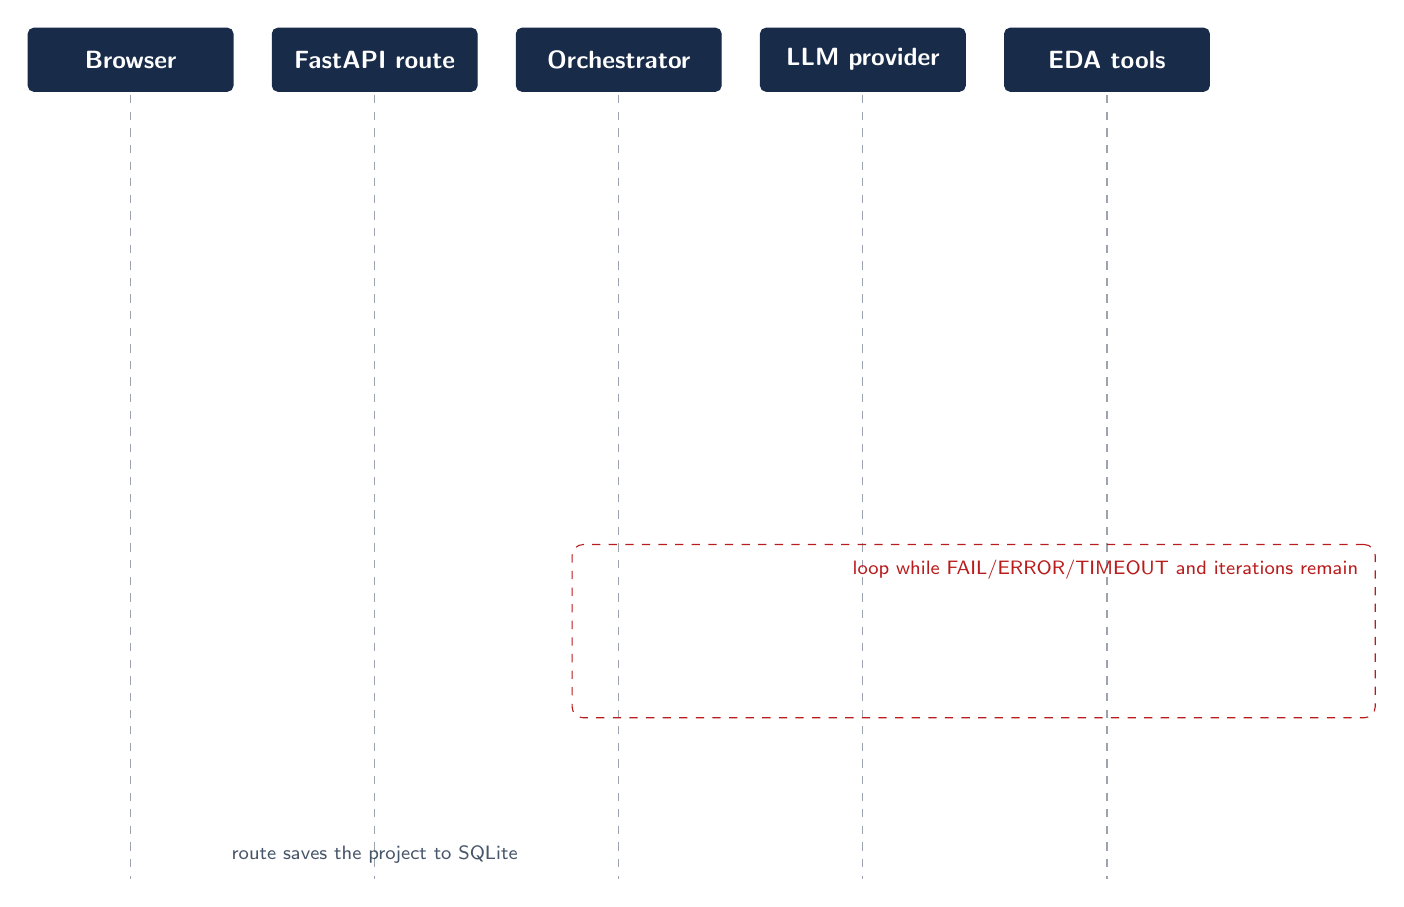
\begin{tikzpicture}[font=\scriptsize]
  \foreach \x/\n/\l in {0/B/Browser,3.1/A/FastAPI route,6.2/O/Orchestrator,9.3/L/LLM provider,12.4/S/EDA tools}{
    \node[hbox,minimum width=2.6cm] (\n) at (\x,0) {\l};
    \draw[midgrey,dashed] (\x,-0.45) -- (\x,-10.4);
  }
  \msg{0}{3.1}{-1.0}{POST /api/design/stream}{}
  \msg{3.1}{6.2}{-1.6}{pipeline\_events()}{}
  \msg{6.2}{9.3}{-2.2}{parse\_intent}{}
  \msg{9.3}{6.2}{-2.7}{RTLDesignSpec}{,dashed}
  \msg{6.2}{0}{-3.1}{SSE: start, intent}{,dashed}
  \msg{6.2}{9.3}{-3.7}{generate\_rtl, generate\_testbench, explain}{}
  \msg{6.2}{0}{-4.3}{SSE: rtl, lint, testbench, explanation}{,dashed}
  \msg{6.2}{12.4}{-4.9}{simulate(): iverilog + vvp}{}
  \msg{12.4}{6.2}{-5.4}{transcript + VCD}{,dashed}
  \msg{6.2}{0}{-5.8}{SSE: simulate (PASS / FAIL / ERROR)}{,dashed}
  \node[draw=badred,dashed,rounded corners,minimum width=10.2cm,minimum height=2.2cm,anchor=north west] (loopbox) at (5.6,-6.15) {};
  \node[anchor=north east,font=\scriptsize,text=badred] at ($(loopbox.north east)+(-0.1,-0.08)$) {loop while FAIL/ERROR/TIMEOUT and iterations remain};
  \msg{6.2}{9.3}{-7.0}{fix\_design (or compiler repair first)}{}
  \msg{6.2}{0}{-7.5}{SSE: fixing, fix}{,dashed}
  \msg{6.2}{12.4}{-8.0}{re-simulate}{}
  \msg{6.2}{12.4}{-9.05}{after a PASS: mutants, Yosys + OpenSTA}{}
  \msg{6.2}{0}{-9.55}{SSE: synthesis, strength, timing, done}{,dashed}
  \node[font=\scriptsize,align=left,text=inkgrey] at (3.1,-10.1) {route saves the project to SQLite};
\end{tikzpicture}}
\caption{Sequence of one streamed run. Solid arrows are calls; dashed arrows are replies and streamed events.}
\label{fig:sequence}
\end{figure}

\section{Step by step}

\begin{enumerate}[leftmargin=*,label=\textbf{Step \arabic*.}]
  \item \textbf{You type and press Generate RTL} (or Ctrl/Cmd+Enter). \code{PromptPanel.submit} rejects an empty prompt or one longer than 2000 characters, clamps the target clock to 1--10000 MHz (the slider itself goes from 10 to 500) and calls \code{App.handleGenerate}.
  \item \textbf{Optional: review the specification.} If ``Review the specification before generating'' is ticked, \code{handleGenerate} first calls \code{api.parseSpec}, which sends \code{POST /api/spec/parse}. The server only runs \code{parse_intent} and returns the specification. The page shows it in the SpecReview panel, you edit the behaviour and constraints, and ``Generate with this specification'' starts the run with that exact specification (Section~\ref{sec:specreview}).
  \item \textbf{The browser opens a stream.} \code{startRun} clears the previous results and calls \code{api.streamDesign}, which sends \code{POST /api/design/stream} with the prompt, target clock, the chosen model, the optional testbench model, the optional confirmed specification, the thinking level, \code{self_correct=true}, \code{max_iterations=5} and \code{timeout_seconds=30}.
  \item \textbf{The server checks the request.} FastAPI validates the JSON against \code{RunRequest} (HTTP 422 if invalid). This includes the model ids (Section~\ref{sec:modelid}) and the bounds on a user specification. \code{design_stream} applies the rate limit, creates a fresh design id with \code{_new_design_id} (a full random UUID) and starts \code{pipeline_events}.
  \item \textbf{Specification.} The orchestrator calls \code{parse_intent}, unless you already confirmed a specification. The model returns JSON describing the module name, parameters, ports (name, direction, width), behaviour and constraints, which is validated as an \code{RTLDesignSpec}. Event \code{intent} is streamed.
  \item \textbf{RTL.} \code{generate_rtl} is called with the specification. The orchestrator checks the reply contains a complete \code{module <name> ... endmodule}; if not, it retries once, then fails clearly. Event \code{rtl}. The linter may add a \code{lint} event.
  \item \textbf{Testbench.} \code{generate_testbench} is called with the specification (by the separate testbench model if you chose one). The result must be a complete module named \code{testbench}, must really instantiate the design and must contain at least one check; otherwise retry once, then refuse. Event \code{testbench}.
  \item \textbf{Explanation.} \code{explain_design} writes 2--3 sentences. If this cosmetic step fails, a placeholder is used and the run continues. Event \code{explanation}.
  \item \textbf{First simulation.} \code{simulator.simulate} scans the code against the sandbox policy, writes the two files, compiles, runs and parses the transcript. The result is recorded as iteration 0. Event \code{simulate}.
  \item \textbf{Self-correction loop} (only if FAIL, ERROR or TIMEOUT): compiler repair or LLM diagnosis, guards, re-simulation, up to \code{max_iterations} times (Chapter~\ref{ch:pipeline}). Events \code{fixing}, \code{fix}, \code{simulate}.
  \item \textbf{Post-processing.} Coverage summary, VCD parsed into a waveform, port-level schematic, generic synthesis (event \code{synthesis}, which also carries the two netlists the Schematic tab draws). If the run passed only after the testbench was changed, the original testbench is run again on the final design, and a fresh second-opinion testbench is requested (event \code{second_opinion}). Then, for a PASS only, testbench strength (event \code{strength}) and the timing and area estimate with its critical path and equivalence proof (event \code{timing}). Chapters~\ref{ch:trust} and~\ref{ch:timing} explain these.
  \item \textbf{Done.} A full \code{RunResponse} is built and sent in the \code{done} event. It records which model wrote the design and, if different, which wrote the testbench. \code{design_stream} saves it to SQLite before forwarding it.
  \item \textbf{The page updates.} For each event, \code{startRun} adds a message to the run timeline in the sidebar and fills the editors and result panels; on \code{done} it loads the final response, switches to the Results tab and refreshes the Projects list.
\end{enumerate}

\section{The event protocol}

Every streamed message is one JSON object with a \code{stage} field. The full list:

\begin{center}
\small
\begin{tabularx}{\textwidth}{@{}>{\ttfamily}lX@{}}
\toprule
\textrm{\textbf{stage}} & \textbf{Meaning and extra fields} \\
\midrule
start & Run started; names the provider and model. \\
intent & Specification ready: \code{rtl_spec}, and \code{fallback_notice} if degraded. \\
rtl & RTL ready: \code{rtl_code}. \\
lint & Lint found something: \code{target} (rtl, tb or fix) and \code{lint} (errors, warnings). Informational only. \\
testbench & Testbench ready: \code{testbench_code}. \\
explanation & \code{explanation} text. \\
simulate & One simulation finished: \code{iteration}, \code{status}, \code{result}. \\
fixing & About to ask the model to diagnose (iteration number). \\
fix & A fix was applied, or the loop stopped: \code{fix_summary}, \code{fix_type} (compiler\_repair, llm\_diagnosis or offline\_scripted), \code{diagnosis}, new code. \\
synthesis & Generic synthesis result or ``not available''. \\
second\_opinion & Sent twice when a repair rewrote the testbench: first ``asking for a fresh testbench'', then \code{second_opinion} (status PASS, FAIL or unavailable, with counts and the model). \\
strength & After a PASS: \code{strength} (bugs injected, bugs caught, survivors). \\
timing & After a PASS, when the tools exist: \code{timing} (slack, area, cells, or the reason it was refused). \\
done & Final verdict: \code{status}, \code{response} (the complete RunResponse, including \code{pass_disputed} when the evidence contradicts a PASS); its message says ``PASS, but disputed: \ldots'' in that case. \\
error & Something failed: a short, safe \code{message}. \\
\bottomrule
\end{tabularx}
\end{center}

% ---------------------------------------------------------------------------
\chapter{The Pipeline and Self-Correction Loop}
\label{ch:pipeline}

All of this lives in \file{backend/orchestrator.py}, mainly in the generator function \code{pipeline_events}. A \textbf{generator} is a Python function that produces values one at a time with \code{yield}; each yielded value here is one event, which is exactly what streaming needs. The one-shot route uses \code{run_pipeline}, which simply consumes the same events and returns the final response.

\section{Validation between stages}

The orchestrator does not pass model output blindly to the next stage:

\begin{description}
  \item[\code{_has_complete_module(code, name)}] True only if the text contains \code{endmodule} and a \code{module <name>} header, both outside comments and strings (a comment such as \code{// module counter} next to \code{module up_counter} used to pass). Catches truncated or chatty answers before they reach the compiler, where they would cause a cryptic syntax error.
  \item[\code{_tb_check_count(tb)}] Counts the places where a testbench can actually fail: increments of a fail or error counter, \code{$error} / \code{$fatal}, \code{assert(} and calls of the standard \code{chk(...)} task. Comments and strings are blanked out first (\code{_strip_comments_and_strings}), so a comment such as \code{// $error} does not count, and a bare \code{fail_count = 0} is not a check. A testbench with zero checks cannot fail, so it is refused: ``Refusing to report PASS from a testbench that cannot fail.''
  \item[\code{_tb_problems(tb, name)}] The full acceptance test for a testbench: a complete module named \code{testbench}, at least one check, and a real instance of the design (\code{_instantiates_dut}), not just a mention of its name. The same rules apply to a testbench proposed by a repair.
  \item[Retry once.] RTL and testbench generation each get one automatic retry when the answer is invalid; a second failure stops the run with a clear message.
\end{description}

\section{The self-correction loop}

\begin{figure}[H]
\centering
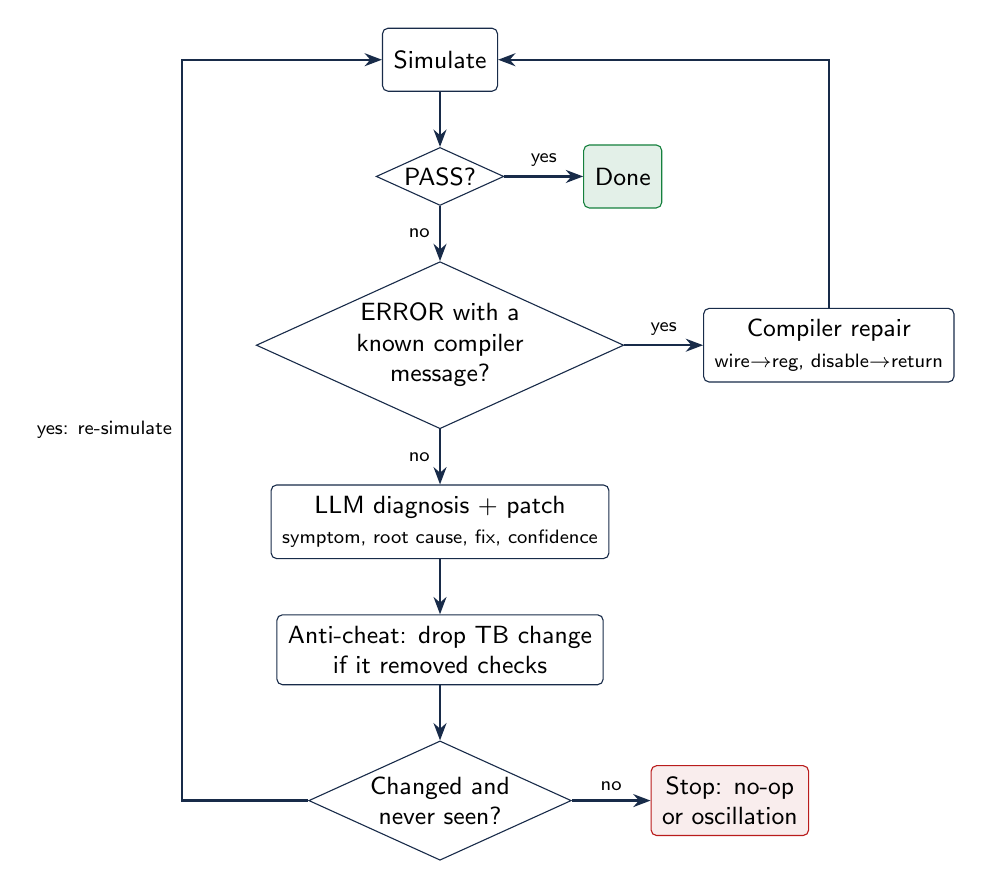
\begin{tikzpicture}[node distance=7mm and 10mm]
  \node[box] (sim) {Simulate};
  \node[diamond,draw=navy,align=center,aspect=2.2,inner sep=1pt,font=\small,below=of sim] (d1) {PASS?};
  \node[okbox,right=of d1] (done) {Done};
  \node[diamond,draw=navy,align=center,aspect=2.2,inner sep=1pt,font=\small,below=of d1] (d2) {ERROR with a\\ known compiler\\ message?};
  \node[box,right=of d2] (cr) {Compiler repair\\ \scriptsize wire$\to$reg, disable$\to$return};
  \node[box,below=of d2] (llm) {LLM diagnosis + patch\\ \scriptsize symptom, root cause, fix, confidence};
  \node[box,below=of llm] (ac) {Anti-cheat: drop TB change\\ if it removed checks};
  \node[diamond,draw=navy,align=center,aspect=2.2,inner sep=1pt,font=\small,below=of ac] (d3) {Changed and\\ never seen?};
  \node[badbox,right=of d3] (stop) {Stop: no-op\\ or oscillation};
  \draw[arr] (sim)--(d1); \draw[arr] (d1)--node[above,font=\scriptsize]{yes}(done);
  \draw[arr] (d1)--node[left,font=\scriptsize]{no}(d2);
  \draw[arr] (d2)--node[above,font=\scriptsize]{yes}(cr);
  \draw[arr] (d2)--node[left,font=\scriptsize]{no}(llm);
  \draw[arr] (llm)--(ac); \draw[arr] (ac)--(d3);
  \draw[arr] (d3)--node[above,font=\scriptsize]{no}(stop);
  \draw[arr] (cr.north) |- (sim.east);
  \draw[arr] (d3.west) -- ++(-1.6,0) |- node[pos=0.25,left,font=\scriptsize]{yes: re-simulate} (sim.west);
\end{tikzpicture}
\caption{One pass of the loop. It also stops when \code{max_iterations} is reached (5 from the UI).}
\end{figure}

The loop condition is:
\begin{lstlisting}[style=plain]
while self_correct and result.status in ("FAIL", "ERROR", "TIMEOUT") and iteration < max_iterations:
\end{lstlisting}
Each pass is recorded as an \code{IterationRecord} (iteration number, status, fix summary, fix type, diagnosis, pass/fail counts, last 1200 characters of the log) so the UI can show a timeline.

\subsection{Deterministic compiler repairs}
\label{sec:compilerrepair}

Some failures are mechanical, and the compiler names the exact problem. Asking an LLM to guess would be slower and less reliable, so \code{_compiler_repairs} fixes two of them directly:

\begin{description}
  \item[\code{_repair_compile_errors} (wire to reg).] Icarus reports \code{design.sv:LINE: error: X is not a valid l-value} when a \code{wire} is assigned inside an \code{initial} or \code{always} block. The function finds the file the compiler blamed and changes only that declaration, \code{wire [3:0] X;} to \code{reg [3:0] X;}.
  \item[\code{_repair_disable_functions} (disable to return).] Icarus rejects \code{disable fname;} used as an early exit inside a function. It is replaced with \code{return fname;}, which Icarus accepts and which keeps the first-match behaviour.
\end{description}

Each repair produces a structured diagnosis with confidence ``high'' and the compiler line as evidence, and is labelled \code{fix_type = "compiler_repair"} so it is never confused with AI reasoning.

\subsection{LLM diagnosis}

Otherwise, \code{fix_design} sends the debugger model the specification (``source of truth''), the RTL, the testbench and the last 4000 characters of the simulator log. The prompt requires the answer in tagged sections:

\begin{lstlisting}[style=plain]
<diagnosis>
symptom: ...        root_cause: ...
fix_location: ...   confidence: high|medium|low
</diagnosis>
<rtl> ...full corrected RTL... </rtl>
<testbench> ...full testbench... </testbench>
<summary> one sentence </summary>
\end{lstlisting}

The prompt also tells the model to check the testbench against the specification first: if the testbench's expected value is wrong, the bug is in the testbench, not the RTL. This rule came from a real live failure (a 32-bit expected value compared with a 3-bit output).

Two things can go wrong with the answer itself, and both are handled honestly. If the reply cannot be read (a refusal, a reply cut off inside \code{<rtl>}, code without the tags), the fixer asks once more with the format spelled out; if the second reply is also unreadable the loop stops with ``The repair reply could not be read'', not with the misleading ``no change''. And if the model stops answering in the middle of the loop (a quota or a timeout), the run is \emph{kept}: the last simulated result, the code and the waveform are returned with the note ``The repair model became unavailable \ldots{} this is the last simulated result''. Before the last review such a failure threw the whole run away.

\subsection{Anti-cheat guard}

The testbench is the judge, so the repair loop must not be able to weaken it. The rule depends on what the last run showed:

\begin{description}
  \item[The testbench did not compile.] Its oracle never ran, so the fixer may rewrite it freely.
  \item[It ran but printed no readable summary] (for example \code{passed = 12} instead of \code{Passed: 12}) and no failure lines. The oracle is broken, so it may be repaired, but the repaired testbench may not have fewer checks.
  \item[Anything else] (a FAIL, a runtime stop such as \code{$fatal}, a hang). The testbench did its job. A proposed testbench with \emph{fewer} checks is thrown away with the note ``Testbench change rejected: it removed self-checks''.
\end{description}

The middle case used to be treated like the first: any ERROR or TIMEOUT unlocked a free rewrite. The last review showed how that could be abused: a testbench that stopped at its first mismatch with \code{$fatal} gave an ERROR, the design model replaced it with a one-check testbench, kept the bug, and got a PASS. Failure lines without a summary are now a FAIL (Section~\ref{sec:verdict}), so that path is closed. A proposed RTL that is not a complete module with the right name, or a proposed testbench that fails \code{_tb_problems}, is also rejected.

When a separate model wrote the testbench (Section~\ref{sec:independenttb}), the rule is stricter: the design model may not change that testbench at all unless its oracle is broken (one of the first two cases). If it does repair it, the result is no longer labelled independent, and a warning says so (``The separate model's testbench did not compile and was repaired by the design model, so the final testbench is no longer independent of the design'').

Even an accepted testbench change leaves a trace. At the end of the run, if the result is PASS and the testbench is no longer the one first generated, the \emph{original} testbench is run again on the final design. If it still fails, the result carries the warning ``The testbench was modified during repair, and the ORIGINAL testbench still reports \ldots{} Review the testbench change before trusting this PASS.'' The verdict itself then changes too: the response gets a \code{pass_disputed} reason and the screen shows \textbf{PASS, disputed} in warning colour with ``Do not trust this PASS yet'' under it. The same happens when the fresh second-opinion testbench fails the final design. Before the last review the headline stayed a plain green PASS and the contradiction was only in the warning text, which is exactly where an examiner would not look.''

\subsection{No-op and oscillation guards}

\code{_state_hash} computes a SHA-256 fingerprint of the RTL and testbench together, after removing comments and all whitespace, so cosmetic edits do not count as changes. If the fix produces the same fingerprint as now, the loop stops (``Model returned no change''). If it produces a fingerprint seen earlier, the loop stops (``Oscillation detected''). Tracking the testbench as well as the RTL matters: a fix that only repairs a wrong expected value in the testbench is a real change.

\begin{viva}
\emph{``What stops the AI from cheating?''} Several things: the testbench is written from the specification, and its prompt tells it the RTL is withheld; a fix may rewrite the testbench freely only when it did not compile, and otherwise may not reduce its checks; if the testbench changed, the original one is run again at the end and a fresh second-opinion testbench is asked for, and if either fails the verdict reads ``PASS, disputed''; with a separate testbench model, a failing check is never rewritten by the design model; the design may not print or end the simulation; and only the simulator's own counts decide the verdict. Also, a fix that changes nothing or repeats an earlier state stops the loop.
\end{viva}

\section{Post-processing}

After the loop, in this order, the orchestrator:
\begin{enumerate}
  \item adds the coverage summary (\code{compute_coverage}), the parsed waveform (\code{parse_vcd}) and the port-level schematic (\code{build_schematic});
  \item runs generic Yosys synthesis if Yosys is installed (if not, the \code{synthesis} event says so; nothing is invented); this also gives the RTL-cell and gate-level netlists for the Schematic tab (Section~\ref{sec:schematicnetlists});
  \item if the run passed but the testbench was changed during repair, re-runs the original testbench and asks for a second opinion (Section~\ref{sec:secondopinion});
  \item for a PASS, measures testbench strength (Section~\ref{sec:strength});
  \item for a PASS, when Yosys, OpenSTA and the cell library are all present, runs the timing and area estimate, which ends with the equivalence proof (Chapter~\ref{ch:timing});
  \item joins every warning (repair stopped because the model became unavailable, a port wider than the check task compares, too few checks, weak testbench, original testbench still failing, second opinion disagrees, the two models disagree, an independent testbench repaired by the design model) into one \code{verification_warning} shown on the result, and sets \code{pass_disputed} when the original or the fresh testbench fails a PASS.
\end{enumerate}
Each extra check is wrapped so that if it fails it only disappears from the result; it can never break a run that already has a verdict. Measured toggle coverage is not a separate stage: the simulator computes it every time it parses a result (Section~\ref{sec:toggle}).

\section{Fallback policy: honest degraded mode}
\label{sec:fallback}

All model calls go through \code{_call_llm} inside \code{pipeline_events}:

\begin{enumerate}
  \item If the run is already offline, call the per-run \code{OfflineProvider}.
  \item Otherwise call the live provider. If it raises an error, \code{_is_upstream_error} decides whether this was the provider's fault (connection error, timeout, rate limit, HTTP 401/403/429/5xx, empty answer). Programming errors are \emph{not} hidden; they surface as errors.
  \item For a provider failure \emph{before any live call has succeeded}, switch this run to offline mode and set a visible \code{fallback_notice}.
  \item For a provider failure \emph{after} a live call succeeded (\code{live_ok}), never switch to the demo. At the repair step the run is kept with the last result (see above); at any other step it fails honestly: ``LLM became unavailable mid-run''. Swapping to a curated design at that point would silently replace your design with an unrelated counter. A specification you confirmed counts as user work, so it sets \code{live_ok} too.
  \item The decision to run offline is made with the provider that serves \emph{the chosen model}, not the default one. Before the last review, a Cloudflare model you picked was silently served by the scripted demo whenever the OpenCode app (the default provider) was missing from the server.
  \item If \emph{you} picked a model in the Model menu (not the server's default) and it fails, the run is never swapped for the scripted demo. \code{_chosen_model_problem} says in plain words why: ``The model you chose (\ldots) could not be used: its usage limit has been reached / it did not answer in time / the provider did not accept the credentials \ldots{} Pick another model from the Model menu.'' The same happens when the separate testbench model fails (``The testbench model you chose \ldots'').
\end{enumerate}

Each run gets its own offline provider instance, so one user's ``buggy demo'' flag cannot leak into another user's run. The helper \code{_invoke} also lets older provider stubs work by dropping the optional \code{reasoning_effort} and \code{spec} arguments only when the function says it does not accept them.

For a demo, this gives a three-step fallback ladder: a live model; then the offline scripted demo (labelled ``Offline demo'' or ``Degraded mode'' on screen); then saved live results opened from the Projects menu. The preflight tool (Chapter~\ref{ch:testing}) checks that all three are ready.

% ---------------------------------------------------------------------------
\chapter{Measuring How Much a PASS Is Worth}
\label{ch:trust}

A PASS only says that the testbench found nothing wrong. It does not say whether the testbench \emph{could} have found something. If the model writes a weak testbench (few checks, wrong expected values, or checks that a repair quietly relaxed), a wrong design can still pass. This chapter describes the five things SiliconScribe does around the loop to show how much a particular PASS is worth.

\begin{analogy}
A student passes a test. Before you trust the mark, you ask: was the test hard enough (strength)? Did it cover the whole syllabus (coverage)? If the teacher changed the answer key halfway through, does a second, fresh paper agree (second opinion)? Was the paper set by someone other than the student (separate testbench model)? Was the question itself what you meant to ask (specification review)?
\end{analogy}

\section{Testbench strength (mutation testing)}
\label{sec:strength}

Mutation testing (Section~\ref{sec:mutation}) is normally run once, by hand, on known designs. \file{backend/mutation.py} runs it automatically on \emph{every} design that passes, using that design's own testbench.

\begin{enumerate}
  \item \code{mask_code} makes a same-length copy of the RTL with comments, strings, compiler directives and parameter declarations blanked out, so nothing in them is ever changed.
  \item \code{candidate_mutants} lists every one-token change the operators can make: an arithmetic, logic or comparison operator swapped (for example \code{+} to \code{-}, \code{&} to \code{|}, \code{==} to \code{!=}, \code{<} to \code{<=}), a \code{~} or \code{!} removed, \code{posedge} swapped with \code{negedge}, a sized constant changed by one, the lowest bit of a binary or hex literal flipped, a 1-bit constant flipped, or an \code{if} condition negated. Bit ranges such as \code{[WIDTH-1:0]} and loop headers are protected: changing them alters a declaration or can create an endless loop, not a realistic bug.
  \item \code{select_mutants} picks up to 12 of them (\code{STRENGTH_MAX_MUTANTS}), spread across the kinds of change and along the file, in a fixed (repeatable) way.
  \item \code{run_strength} first runs the \emph{unmutated} design with the same testbench and times it (the baseline). Then it simulates the same testbench against each mutant, with 6 seconds per mutant and a 40-second budget overall (\code{STRENGTH_BUDGET_SECONDS}). A mutant that does not compile says nothing and is not counted. A mutant the testbench \emph{reports as failing} is \textbf{caught}; one that still passes \textbf{survived}. A mutant that times out counts as caught only if the baseline finished in well under the limit (the mutant made the design hang); otherwise, like a crash, it is \textbf{inconclusive} and not counted.
\end{enumerate}

The result is shown as ``Caught N of M injected bugs'', with each survivor's line number and change. If the time budget runs out, the score is marked as stopped early.

\begin{warnbox}
A survivor is ``not noticed'', not ``proven missed'': some mutants are \textbf{equivalent} (the changed design behaves exactly like the original), so no testbench could catch them. The sample is small and syntactic. The score is evidence about the testbench, not a proof. When at least 5 mutants ran and fewer than half were caught, \code{weak_strength_note} adds a ``Weak testbench'' warning to the PASS; for a small design with fewer than 5 mutants it warns when \emph{none} was caught. Before the last review, a slow testbench with a single check scored 3 of 3 because every mutant ran out of time, and a small design that caught 0 of 3 got no warning at all.
\end{warnbox}

\section{Measured toggle coverage}
\label{sec:toggle}

Coverage asks how much of the design the tests exercised. SiliconScribe measures one kind directly: \textbf{toggle coverage}. A bit is covered when the simulator recorded it going from 0 to 1 \emph{and} from 1 to 0. A bit that never moved was never really tested.

\code{toggle_coverage} in \file{backend/vcd_parser.py} reads the VCD file the simulator wrote (not anything the testbench prints). It counts only signals inside the \emph{design's own} instance: the simulator first finds, in the testbench text, the instance names of modules defined in the RTL (\code{dut_instance_names}), and only signals below one of those instances count, also when the design sits inside a wrapper module or a \code{generate} block. Testbench variables and testbench-side helper modules cannot inflate the number (before the last review, an unrelated stimulus generator in the testbench raised an adder's coverage from 46\% to 77\%). Each run deletes the previous run's waveform first, so an old file can never be measured for a new run. A change through \code{x} or \code{z} does not count. The result is a percentage of bits, the number of bits and signals, and up to 12 signals that never switched (with the bit positions that never rose or never fell). If the VCD was larger than the 8 MB read limit, the figure is marked as a lower bound.

\begin{warnbox}
Only toggle coverage is measured. Line and branch coverage are not. Verilator was tried for them and rejected: with the pip-installed Verilator only 3 of 12 evaluated designs built, and the testbenches of two designs (c3, c4) stopped with ``unsupported tristate construct''. The older \code{compute_coverage} summary (vectors, pass rate, any \code{COV:} lines a testbench prints) is still there, but it only repeats what the testbench reported.
\end{warnbox}

\section{The second opinion}
\label{sec:secondopinion}

The weakest kind of PASS is one that only appeared after a repair \emph{rewrote the testbench}. Maybe the repair fixed a wrong expected value (good). Maybe it relaxed a correct check (bad). The simulator cannot tell which.

So, when the final status is PASS and the testbench is no longer the one first generated, the orchestrator asks for a \textbf{fresh testbench} from the same specification (by the same testbench model), checks it with \code{_tb_problems}, and runs the final design against it. There are three outcomes:
\begin{description}
  \item[Agrees] The fresh testbench passes: ``Second opinion agrees: a fresh testbench, written from the same specification, passes all N of N checks.''
  \item[Disagrees] The fresh testbench fails: the PASS becomes ``PASS, disputed'' and a warning names the failing count.
  \item[Unavailable] The fresh testbench could not be generated, was unusable, did not run cleanly, or ran fewer than 20 checks (too few to count as agreement; a one-check testbench used to count). The reason is shown; nothing is assumed.
\end{description}
The second opinion is skipped in offline mode (the scripted demo has nothing new to say) and can be turned off with \code{SECOND_OPINION_ENABLED=0}.

A real example (s2 prompt, an 8-bit loadable up/down counter, model hy4-flash-free): PASS 8672/8672 after one repair that rewrote the testbench. The fresh testbench also passed (8517/8517), while the original testbench still failed, which was shown as a warning. A hand-written reference then gave 0 mismatches in 40,027 cycles: the design was correct and the original testbench was wrong.

\section{A separate model for the testbench}
\label{sec:independenttb}

By default one model writes both the design and the testbench. Withholding the RTL from the testbench step removes the most direct circular check, but one risk remains: if the model misreads the specification, it can misread it the same way twice, and the wrong design and the wrong testbench agree.

The ``Testbench written by'' menu lets a \emph{different} model, even from a different provider, write the testbench (\code{testbench_model} in the request). Then three rules change:
\begin{itemize}
  \item The design model is \textbf{never} allowed to change the testbench to make a failing check go away: a failing check is reported, not rewritten. Only a testbench whose oracle is broken (it did not compile, or printed no readable summary) may be repaired, and then the result is no longer labelled independent. Two spellings of the same model (\code{x-free} and \code{opencode/x-free}) are not counted as independence.
  \item If the two models disagree (the run ends in FAIL), the result says so and names both models: ``Either the design or the testbench misreads the specification: compare the first failing check with the specification before changing either.''
  \item The result records both models (``Design written by \ldots. Testbench written by \ldots, a separate model''); with one model it says ``Design written by \ldots, which also wrote the testbench''.
\end{itemize}

\begin{keyidea}
Independence makes failures more honest, not passes more frequent. A real example: design by opencode/hy4-flash-free, testbench by nim/poolside/laguna-xs-2.1, 4-bit counter: FAIL 124/146. The counter was correct; the testbench sampled one cycle early. The app refused to pass it and reported that the two models disagree. With one model, a repair could have quietly ``fixed'' either side.
\end{keyidea}

It costs one more model call per run, and with the free models tried it was not reliable enough to be the default, which is why it is an option.

\section{Reviewing the specification}
\label{sec:specreview}

Everything is built from the specification, and the specification is written by the model. If it is wrong (wrong reset polarity, a missing flag), both the design and the testbench will follow it. ``Review the specification before generating'' puts you in the loop at that point:
\begin{enumerate}
  \item \code{POST /api/spec/parse} runs only \code{parse_intent} and returns the specification.
  \item The SpecReview panel shows the module name, the ports table and parameters, and lets you edit the behaviour text and the constraints (one per line).
  \item ``Generate with this specification'' sends it as \code{spec} in the run request. The orchestrator then skips \code{parse_intent} and uses exactly that specification.
\end{enumerate}

A specification from the browser is untrusted input: its names end up in file patterns and prompts. \code{check_user_spec} therefore requires plain identifiers for the module, port and parameter names, 1 to 64 ports, at most 16 parameters, at most 4000 characters of behaviour and at most 30 constraints of 500 characters. The specification actually used is shown read-only on the Results tab under ``Specification the design was built from''.

% ---------------------------------------------------------------------------
\chapter{The Timing and Area Estimate}
\label{ch:timing}

Simulation answers ``does the design do the right thing?''. A chip designer also asks ``how big is it?'' and ``how fast can it run?''. After a PASS, \file{backend/timing.py} gives an early answer to both, using two free tools and a real cell library.

\section{The idea in plain words}

\begin{description}
  \item[Standard cells.] A chip is built from a library of small, pre-designed blocks called \textbf{standard cells}: a NAND gate, an inverter, a flip-flop, and so on. A foundry publishes, for each cell, its area in square micrometres and how long a signal takes to pass through it. That data lives in a \textbf{liberty file} (\file{.lib}).
  \item[sky130.] SiliconScribe uses the open \textbf{SkyWater 130 nm} library, high-density variant (\code{sky130_fd_sc_hd}), at its \textbf{typical corner}: 25\,\textdegree C and 1.8 V. The file is \file{backend/pdk/sky130hd_tt.lib}.
  \item[Mapping (Yosys).] \textbf{Yosys} turns the RTL into a \textbf{netlist}: a list of real sky130 cells and the wires between them. Adding up the cells' areas gives the \textbf{mapped area}.
  \item[Timing (OpenSTA).] \textbf{OpenSTA} is a \textbf{static timing analysis} tool. It does not simulate. It adds up the cell delays along every path from a flip-flop (or input) to the next flip-flop (or output) and compares the longest one, the \textbf{critical path}, with the clock period. The margin left over is the \textbf{slack}: positive means the logic is fast enough for the target clock, negative means it is too slow.
\end{description}

\begin{analogy}
A clock period is the time between two drum beats. Every signal must finish its journey through the gates before the next beat. Slack is how many nanoseconds early the slowest signal arrives. A slack of +9.27 ns at 100 MHz (a 10 ns beat) means the slowest path takes only about 0.73 ns.
\end{analogy}

\section{What one run does}

\code{run_timing(rtl, module, work_dir, target_mhz, testbench_code)} never raises; every outcome is a \code{TimingReport}.
\begin{enumerate}
  \item \textbf{Check the tools}: Yosys and OpenSTA on the PATH and the liberty file present (\code{missing_requirements}). If anything is missing, the run simply has no timing section.
  \item \textbf{Check the input}: a legal module name, the same sandbox scan as simulation, and at most 200 KB of RTL.
  \item \textbf{Apply parameter overrides.} If the testbench instantiates the design as \code{mux #(.WIDTH(16)) dut} or \code{alu #(8) dut}, \code{parameter_overrides} reads those plain numbers (positional ones are matched to the parameters the design declares) so the circuit timed is the circuit that was simulated. Expressions are never guessed; they are reported as ``not applied''.
  \item \textbf{Map with Yosys} (\code{_map_with_yosys}): read the design, \code{proc; tribuf} (so a tri-state survives as a cell that can be detected), \code{synth -flatten} (hierarchy is flattened, so area covers every sub-module), map flip-flops and logic to sky130 cells (low-power isolation cells excluded), write the statistics and \file{netlist.v}.
  \item \textbf{Read what was really built} (\code{analyze_netlist}): which input ports drive the flip-flops' clock pins, whether any unmapped cell, latch or clock-gating cell is present.
  \item \textbf{Refuse instead of guessing} (next section).
  \item \textbf{Time with OpenSTA}: write a small script that reads the library and netlist, creates one clock per clock port found in the netlist at the target period, sets input and output delays to zero, and reports the worst setup path. A design with no flip-flops is timed against a virtual clock, so the answer is its longest input-to-output path.
  \item \textbf{Parse the report} (\code{parse_mapped_stats}, \code{parse_sta}): area, sequential area, cell count, flip-flops, the most common cell types, worst slack, maximum frequency ($1000 / (\text{period} - \text{slack})$ MHz), the critical path's start, end and delay, and its pin-by-pin rows (\code{critical_path_rows}, Section~\ref{sec:critpath}).
  \item \textbf{Prove the netlist equals the RTL} (\code{prove_equivalence} in \file{equivalence.py}, Section~\ref{sec:equivalence}). This runs unless \code{EQUIVALENCE_ENABLED=0}. If the proof itself crashes, the timing numbers stay and the line says the check could not be run.
\end{enumerate}

\section{Clocks come from the netlist}

It would be easy to guess the clock from a port name such as \code{clk}. \file{timing.py} does not. It reads the mapped netlist and takes whatever input port is actually wired to the flip-flops' clock pins, whatever its name. A design with several clocks gets one clock each. Every clock's own paths are timed, \emph{including} the paths from the inputs and to the outputs of that clock's flip-flops; only paths that cross from one clock to another are not timed, and the note says so.

\begin{warnbox}[A bug the last review found here]
Input and output delays used to be attached only to the first clock. Paths from the inputs into the second clock's flip-flops were therefore not timed at all, so a slow multiplier on a second clock was reported as meeting 500 MHz (slack $+1.74$ ns) when on its own it misses by 1.43 ns. Now every clock gets its own input and output delays.
\end{warnbox}

\section{When the estimate refuses}

Some designs cannot be timed honestly with this simple setup. For them the report gives a reason instead of a number:
\begin{itemize}
  \item \textbf{tri-state buffers}: Yosys would otherwise quietly turn them into plain wires, so the circuit timed would not be the one simulated;
  \item \textbf{latches}: latch-based timing is not estimated;
  \item \textbf{combinational loops}: path timing is not defined (OpenSTA reports a disabled loop edge);
  \item \textbf{derived or gated clocks}: a flip-flop clocked by internal logic or a clock-gating cell rather than an input port;
  \item \textbf{no logic cells}: a design that maps to only wires or constants has nothing to time;
  \item \textbf{not synthesizable as written}: Yosys could not map it.
\end{itemize}

\section{What the numbers are, and are not}

\begin{warnbox}[Pre-layout estimate: not sign-off]
The app prints this with every result: one typical corner; no placement or routing, so \textbf{no wire delay}; an ideal clock (no clock tree); zero input and output delays; \textbf{setup analysis only} (hold needs a real clock tree to mean anything). \textbf{Power is not reported.} Real chips are checked after place and route, at several corners. So this answers ``is this logic anywhere near the target clock, and roughly how big is it?'', nothing more. Never present it as final (sign-off) timing or as the area of a manufactured chip.
\end{warnbox}

Two numbers need care. The maximum frequency is computed as $1000 / (\text{period} - \text{slack})$, which is only right when the worst path takes one whole clock period. When the worst path starts or ends on the falling clock edge (a half-cycle path), that formula gives a number that changes with the target clock, so no maximum frequency is shown at all. And a design without a clock is timed against a virtual clock: its longest input-to-output delay is a real number, but $1/\text{delay}$ is not a clock rate, so the chat message does not quote one.

The cell counts come from Yosys' statistics. Yosys writes large areas in exponent form (\code{1.6E+03} for a group of 64 flip-flops), and the parser used to skip such lines, so a 64-bit register was refused as ``no logic cells'' and larger counters reported 0 flip-flops; it now reads exponent numbers. If the testbench sets parameters with \code{defparam}, the note says that those values were \emph{not} applied, so the numbers are for the design's default parameters.

Examples from the built-in designs: the 4-bit counter maps to 11 cells, 150.144\,\umsq{}, minimum period 0.727 ns (meets 100 MHz with +9.27 ns slack); the 8-bit ALU has no clock, 109 cells, 636.861\,\umsq{}, longest path 2.69 ns. The live-generated FIFO (s6) is 120 cells, 1830.51\,\umsq{}, minimum period 1.845 ns.

\section{The critical path, pin by pin}
\label{sec:critpath}

OpenSTA's report lists the worst path as a column of rows, one per pin the signal passes. \code{parse_sta} picks the path block with the smallest slack, and \code{critical_path_rows} turns its data part into rows of five fields: the \textbf{pin} (for example \code{_127_/X}, output X of cell number 127), the sky130 \textbf{cell} type with the library prefix removed (\code{maj3_1}), whether the signal \textbf{rises or falls} there, the \textbf{incremental delay} added by that stage, and the \textbf{arrival} time so far. Rows after ``data arrival time'' (the clock side of the check) are not part of the data path and are dropped; at most 60 rows are kept. The rows travel to the browser in \code{TimingReport.critical_path}.

On the built-in 8-bit ALU (no clock) the worst path starts at input \code{b[0]}, goes through one \code{nor2b_1}, then six \code{maj3_1} cells in a row (a 3-input majority gate is exactly the carry logic of a full adder, so this is the ripple-carry chain, about 0.36 to 0.39 ns per stage), then \code{o21ai_0} and \code{o22ai_1}, and ends at the output \code{overflow} after 2.69 ns. Section~\ref{sec:readtiming} shows how to read this in the app.

\section{Formal equivalence: proving the netlist is the RTL}
\label{sec:equivalence}

The timing and area numbers describe \file{netlist.v}, the mapped netlist. They are only worth something if that netlist is the design that was simulated. \file{backend/equivalence.py} checks this with a formal proof (Section~\ref{sec:formalbasics} explains the ideas). It uses only Yosys and its built-in SAT solver; no external solver is installed.

\code{prove_equivalence(work_dir, module, liberty, params)} runs in the timing stage's own folder, which already holds \file{design.sv} and \file{netlist.v}:
\begin{enumerate}
  \item \textbf{Read the RTL as ``gold''}: \code{read_verilog -sv design.sv}, the \emph{same parameter overrides} the netlist was mapped with (\code{hierarchy -chparam}), \code{proc}, \code{flatten}, and \code{memory}. The \code{memory} pass turns arrays and lookup tables into plain logic and registers, as synthesis does, so such designs are proven instead of skipped.
  \item \textbf{Read the netlist as ``gate''}: first \code{read_liberty} on the sky130 library, so every cell's behaviour comes from the logic function written in the liberty file itself, not from a model someone typed by hand. Then \code{read_verilog netlist.v} and \code{flatten}.
  \item \textbf{Decide the method}: if the netlist contains a sky130 flip-flop cell, the design is sequential; otherwise it is combinational.
  \item \textbf{Combinational: miter and SAT.} \code{miter -equiv} builds one circuit that feeds the same inputs to gold and gate and raises a flag if any output differs. \code{sat -prove-asserts -set-def-inputs -enable_undef} asks the solver whether any input can raise the flag. Inputs are limited to real 0 and 1 values (\code{x} is not a value a real input pin carries), and outputs where the RTL itself says ``don't care'' (\code{x}) are not compared. ``SUCCESS'' means proven over every input value; ``FAIL'' means the solver found inputs where they disagree.
  \item \textbf{Sequential: induction.} \code{equiv_make} pairs the registers of gold and gate by name, \code{async2sync} turns asynchronous resets into a form the prover handles, then \code{equiv_simple -seq 5} and \code{equiv_induct -seq 5} try to prove every pair and every output by temporal induction. \code{equiv_status} reports how many points were proven.
\end{enumerate}

\code{interpret} turns Yosys' output into one of four results, stored as \code{TimingReport.equivalence} with a plain sentence in \code{equivalence_method}:
\begin{description}
  \item[\code{proven}] Combinational: ``SAT proof over every input value''. Sequential: every register and output point proven by induction.
  \item[\code{different}] The solver found input values where the netlist and the RTL disagree. The app shows a red alert and declares the timing and area invalid.
  \item[\code{not_proven}] Induction proved only some points. This usually means synthesis re-encoded the state of a state machine, so registers no longer pair by name. It is also the result, with the reason, when a netlist flip-flop uses a clock edge the RTL does not use, when there are several clocks, or when a register gets a starting value from its declaration or an \code{initial} block (\code{_sequential_limits}): induction would otherwise ``prove'' those wrongly. It is never shown as a pass.
  \item[no result] Yosys could not run the check, the design has more than 600 mapped cells (the proof is skipped: SAT on a large multiplier can run for minutes), or the proof took longer than 20 seconds and was stopped. The app shows ``Netlist not formally checked'' with the reason, never a silent gap.
\end{description}

\textbf{Measured result.} On the 14 evaluated designs plus 4 built-in designs (18 in all): 16 \textbf{proven}, 2 \textbf{not proven} (f1 and f2, the two state machines, whose state was re-encoded by synthesis) and 0 different. A deliberately sabotaged netlist, with one NAND gate swapped for a NOR, was reported as different. The proof shows netlist $=$ RTL for those 16 designs; it says nothing about whether their RTL meets the prompt.

\begin{warnbox}[What the proof does not cover]
It does not prove that the RTL is correct; a bug in the RTL is copied faithfully into the netlist. ``Not proven'' is an honest ``don't know'', not a hidden failure: for f1 and f2 the gate-level simulation check below still passed with the same testbench. The last review checked the proof's blind spots directly: a netlist with one flip-flop moved to the falling clock edge, and a design whose register started at 5 from its declaration, were both ``proven'' before; both are now ``not proven'' with the reason.
\end{warnbox}

\section{How the estimate itself was checked}

\file{backend/tools/verify_mapping.py} checks the timing stage with three tests that do not read the number they check from the same place:
\begin{enumerate}
  \item \textbf{Gate-level simulation}: Yosys writes simulation models of the sky130 cells straight from the liberty file; the mapped netlist is simulated in Icarus with the \emph{same} testbench as the RTL and must give identical Passed/Failed counts. This shows the netlist computes what the RTL computes.
  \item \textbf{Area recount}: area and cell count are recomputed from \file{netlist.v} and the liberty file and compared with what \code{run_timing} reported.
  \item \textbf{Timing sanity}: the design is timed at a second target; the implied minimum period ($\text{period} - \text{slack}$) must not change.
\end{enumerate}
On 19 designs (the 5 built-in ones and the saved evaluation designs) all 19 gave identical pass counts in gate-level simulation. A design the estimate refuses on purpose is reported as REFUSED with its reason, not as a failure. The checker was also given deliberately broken netlists and caught them.

The two checks complement each other: the simulation covers every design, including the state machines, but only the testbench's inputs; the proof covers every input value, but cannot always finish for re-encoded state.

\section{The tool versions}

Yosys 0.71 runs as a WebAssembly build installed with \code{yowasp-yosys}, reached through a small \code{yosys} shim in \file{~/.local/bin}. OpenSTA 3.2.0 was built from source (\file{backend/tools/build_opensta.sh}) and is reached as \code{sta}. The orchestrator runs timing only when \code{TIMING_ENABLED} is on (the default) and \code{missing_requirements()} is empty. \code{POST /api/timing/run} runs the same function on its own.

% ---------------------------------------------------------------------------
\chapter{The LLM Service}
\label{ch:llm}

\file{backend/llm_service.py} talks to the AI providers; \file{backend/model_catalog.py} decides which models the Model menu offers. No other file knows about providers.

\section{Choosing the default provider}

At start-up, \code{_make_provider} reads environment variables (from \file{backend/.env}, which wins over stale shell variables) and picks, in order:

\begin{center}
\small
\begin{tabularx}{\textwidth}{@{}clX@{}}
\toprule
\textbf{Priority} & \textbf{Provider} & \textbf{Selected when} \\
\midrule
0 & Offline & \code{OFFLINE_MODE=1} (always wins, even if keys are set). \\
1 & OpenCode app & \code{LLM_PROVIDER=opencode-app} and the \code{opencode} command exists. Model from \code{LLM_MODEL}. This is the set-up used for the live demo and evaluation. \\
2 & OpenCode Zen & \code{OPENCODE_API_KEY} or \code{ZEN_API_KEY} is set. Model from \code{ZEN_MODEL} or \code{LLM_MODEL}. \\
3 & NVIDIA (older single-model path) & \code{NVIDIA_API_KEY} is set. \\
4 & OpenAI or compatible & \code{OPENAI_API_KEY} is set; add \code{OPENAI_BASE_URL} for OpenRouter, Groq, a local server, etc. \\
5 & Offline & Nothing configured. \\
\bottomrule
\end{tabularx}
\end{center}

Placeholder values such as \code{your_key_here} are treated as empty. Rows 2--4 are an \code{OpenAIProvider}, configured with a base URL and model name.

\section{The OpenCode app provider}

OpenCode is a coding assistant app that the user installs and signs in to with their own account; its free models are meant to be used from inside the app. \code{OpenCodeAppProvider._chat} therefore drives the app's own scripting command instead of imitating its API:
\begin{lstlisting}[style=plain]
opencode run -m <model> --agent plan --archived --format json "<prompt>"
\end{lstlisting}
Every call runs in a fresh, empty temporary folder with the read-only \code{plan} agent (change it with \code{OPENCODE_AGENT}), and with an environment that has the Cloudflare and NIM credentials removed (\code{model_catalog.child_env}). The JSON lines the app prints are read; the text parts become the answer, an error event becomes an upstream error. It is a local, single-user convenience: not something to expose on a public server.

\section{Model routing: one menu, three sources}
\label{sec:routing}

Each run can use a different model, chosen in the Model menu. The model id itself says which provider serves it; \code{get_provider(model)} routes it:

\begin{center}
\small
\begin{tabularx}{\textwidth}{@{}lp{3.7cm}X@{}}
\toprule
\textbf{Id looks like} & \textbf{Served by} & \textbf{Notes} \\
\midrule
\code{opencode/deepseek-v4.1-flash-free} & The configured provider (normally the OpenCode app) & Every model the installed app lists with \code{opencode models}, about 460. A model counts as free only when its name ends in \code{-free} or \code{:free}; the rest are hidden behind ``Show other models'' and are never claimed to be paid, because the price cannot be known from here. \\
\code{github-copilot/auto} & The OpenCode app, after Copilot is connected in it & On the Free and Student plans only ``auto'' exists: GitHub picks the model and does not say which, so the result cannot name its model and runs are not reproducible. It uses your Copilot allowance. \\
\code{@cf/openai/gpt-oss-120b} & \code{CloudflareProvider} (Cloudflare Workers AI) & Live catalogue of text-generation models on your account (40 when checked). Needs \code{CLOUDFLARE_ACCOUNT_ID} and \code{CLOUDFLARE_API_TOKEN}. \\
\code{nim/poolside/laguna-xs-2.1} & \code{NimProvider} (NVIDIA NIM hosted API) & Live catalogue of chat models (15 when checked); the \code{nim/} prefix keeps them apart from OpenCode's own \code{nvidia/...} ids and is removed before the request. Needs \code{NVIDIA_NIM_API_KEY} (a key starting \code{nvapi-}); no other NVIDIA variable is read for this. \\
\bottomrule
\end{tabularx}
\end{center}

Cloudflare and NIM both use the same OpenAI-compatible chat code as every other provider. They get no \code{reasoning} request field (both are strict about unknown fields) and no per-stage model routing (the \code{LLM_MODEL_<STAGE>} variables name OpenCode models). If one of them is chosen but not set up, the run stops with ``Cloudflare is not set up\ldots'' or ``NVIDIA NIM is not set up\ldots''.

\begin{keyidea}
Keys live only in \file{backend/.env} (git-ignored) or the environment of the terminal that starts the backend. The web page never asks for, stores or receives a key. \code{cloudflare_status} and \code{nim_status} return models and hints, never the key. Simulation, synthesis and timing tools get a scrubbed environment, and the OpenCode app gets an environment without the Cloudflare and NIM credentials.
\end{keyidea}

\section{The model catalogue (\texttt{model\_catalog.py})}

\begin{description}
  \item[\code{opencode_models}] Runs \code{opencode models} in an empty temporary folder (40 s limit) and parses the \code{provider/model} lines with \code{parse_opencode_models}: free ones first within each provider, GitHub Copilot entries carry the note above. A good listing is cached for 10 minutes, a failed one for 30 seconds.
  \item[\code{cloudflare_status}] Reads up to 5 pages of Cloudflare's model search, keeps text-generation models, and caches them for 30 minutes. If the list cannot be read it shows a short suggested list with a hint saying so.
  \item[\code{nim_status}] Reads NVIDIA's \code{/models} list and drops entries that are not chat models (embeddings, speech, safety classifiers, image models) and one known to answer 404. Models that answered quickly in a live test are listed first.
  \item[\code{list_models}] (in \file{llm_service.py}) Combines the three: the OpenCode list (free ones only unless \code{include_paid}), then Cloudflare, then NIM, plus a \code{providers} list saying which tabs are available and why not. The configured default model is always first. \code{GET /api/models?refresh=true} re-reads all catalogues and is rate limited, because it calls out.
\end{description}

Model names change often (NVIDIA retired DeepSeek V4.1 Flash on 16 Nov 2026 with HTTP 410), which is why the menu reads the catalogues live instead of a hand-written list.

\section{Checking model ids}
\label{sec:modelid}

A model id from the browser ends up as an argument of a subprocess (\code{opencode run -m <id>}) or part of a URL. An id starting with \code{-} could be read as a command-line flag. So every id must match
\begin{lstlisting}[style=plain]
^[A-Za-z0-9@][A-Za-z0-9._:/@+-]{0,99}$
\end{lstlisting}
(no leading dash, no spaces or shell characters, at most 100 characters). The check is done twice: by Pydantic on every request (\code{model} and \code{testbench_model}) and again by \code{is_valid_model_id} just before the subprocess is started.

\section{One chat call: \texttt{OpenAIProvider.\_chat}}

\begin{enumerate}
  \item \textbf{Pick the model.} A model the user chose in the UI (if different from the default) wins; otherwise the stage-specific model from \code{LLM_MODEL_INTENT}, \code{_RTL}, \code{_TESTBENCH}, \code{_EXPLAIN} or \code{_FIX}; otherwise the default (or the cheaper ``mini'' model for the explanation).
  \item \textbf{Control hidden reasoning.} If no reasoning effort was requested, send \texttt{reasoning: \{enabled: false\}}, because hidden reasoning tokens count against the answer budget. Gateways that reject this field get one retry without it.
  \item \textbf{Send} with the configured timeout (default 120 s, \code{LLM_TIMEOUT_SECONDS}) and token budget (default 8192, \code{LLM_MAX_TOKENS}).
  \item \textbf{Classify failures.} Provider errors are re-raised with the prefix \code{LLM_UPSTREAM:} so the orchestrator can recognise them.
  \item \textbf{Reject bad answers.} If the model stopped because it hit the token limit (\code{finish_reason = "length"}) or returned empty content, raise an error. The code deliberately never uses the model's hidden reasoning text as an answer; that once produced a half-written function shipped as a testbench.
\end{enumerate}

\section{The five stage functions}

\begin{center}
\small
\begin{tabularx}{\textwidth}{@{}lcX@{}}
\toprule
\textbf{Function} & \textbf{Temp.} & \textbf{What it sends and returns} \\
\midrule
\code{parse_intent} & 0.3 & The prompt; returns JSON validated as \code{RTLDesignSpec}. \\
\code{generate_rtl} & 0.2 & Module name, parameters, ports, behaviour, constraints, optional target frequency; returns the extracted module. \\
\code{generate_testbench} & 0.3 & The same specification, \emph{without the RTL}, with an explicit note that the RTL is withheld; returns the extracted testbench. \\
\code{explain_design} & 0.5 & The RTL; returns 2--3 sentences. \\
\code{fix_design} & 0.2 & Spec, RTL, testbench, last 4000 log characters; returns new code, summary, diagnosis, \code{fix_type = "llm_diagnosis"}. \\
\bottomrule
\end{tabularx}
\end{center}

The full system prompts are in \file{backend/llm_service.py} (and Appendix~B of the project report). The testbench prompt insists on Icarus-compatible Verilog-2001, a top module named \code{testbench}, a reset sequence first, directed corner cases plus exhaustive testing when there are at most 4096 input combinations (otherwise at least 100 random vectors), every comparison through the standard \code{chk} task (which uses \code{===} and prints one \code{CHK|...} line per check), the exact \code{Passed:}/\code{Failed:}/\code{ALL TESTS PASSED} summary lines, and a watchdog that prints a failure and stops a hung run.

\section{Reading the model's answer}
\label{sec:llmparse}

Models wrap code in prose and Markdown fences, think out loud first, and sometimes give a draft before the real answer. The parsers are forgiving, but in a careful order:

\begin{description}
  \item[\code{_strip_think}] Removes reasoning blocks (\code{<think>...</think>}), and everything before a lone closing \code{</think>} (some models print only the closing tag). Every parser below starts with this, so a draft written while ``thinking'' is never taken as the answer.
  \item[\code{_strip_code_fence}] Finds every complete \code{module ... endmodule} unit in the whole reply and keeps \emph{one definition per module name: the last one} (\code{_last_definition_of_each}). A reply with a draft and then a ``corrected'' copy used to produce the module twice, which Icarus rejects as ``already declared''; helper modules with other names are all kept.
  \item[\code{_extract_json}] Takes the \emph{last} complete top-level JSON object in the reply that parses, accepting raw newlines inside strings (models often paste Verilog into JSON without escaping). The old ``first brace to last brace'' slice broke on prose such as ``\{as requested\}'' before the JSON, or on a draft object followed by the final one.
  \item[\code{_parse_fix_response}] Reads the \emph{last} \code{<diagnosis>}, \code{<rtl>}, \code{<testbench>} and \code{<summary>} sections (a model that first restates the format inside its reasoning no longer fools it); falls back to JSON, then to \code{_salvage_fix_json}, which recovers each field by locating the next known key. If none of these yields any code, the answer is marked \code{parse_failed} (Section~\ref{ch:pipeline} describes the one retry).
\end{description}

The specification model is also forgiving about spelling: port directions such as \code{Output}, \code{out} or \code{in} are normalised, a missing description becomes empty text, a behaviour given as a list is joined, and a single constraint string becomes a list. A module name written by the model is turned into a plain identifier (\code{model_module_name}: \code{Up/Down Counter} becomes \code{Up_Down_Counter}, and \code{testbench}, which would collide with the testbench's own module, becomes \code{testbench_dut}). A name \emph{you} type in the specification review is not rewritten; it is checked and refused with a clear message if it is not a plain identifier.

When a call fails, the reason shown is read with whole-word patterns (\code{_reason}): HTTP 429 or ``too many requests'' is a usage limit; 410 or ``retired'' means the provider retired the model; an empty answer after reasoning means the model spent its whole answer budget on thinking; a missing \code{opencode} command is reported as such. The earlier substring tests gave wrong reasons, for example ``credentials'' for any message that contained \code{max_tokens}. The HTTP client retries a failed call twice (\code{LLM_MAX_RETRIES}); three retries with a 120-second timeout could make one call wait eight minutes.

\section{The offline provider}

\code{OfflineProvider} needs no internet. It is used when \code{OFFLINE_MODE=1}, when nothing is configured, or as the labelled fallback described in Chapter~\ref{ch:pipeline}. It matches whole words in the prompt (\code{match_design}): ``alu'' with ``8-bit'' gives the 8-bit ALU, then ``alu'', ``counter'', ``adder'' or ``mux'' (plurals allowed); anything else defaults to the counter, with a notice saying the request did not match. Whole words matter: plain substring matching sent ``8-bit counter with a load \emph{value}'' to the ALU (``value'' contains ``alu'') and ``dis\emph{count} calculator'' to the counter, both labelled as exact matches. A ``half adder'' is answered with the built-in full adder but labelled as not an exact match. A prompt containing ``buggy'' gets the counter with a deliberate bug (counting by two), which demonstrates the repair loop. Its ``fix'' simply swaps in the known-correct design, so it reports \code{fix_type = "offline_scripted"} and \emph{no} diagnosis, because inventing a root cause would be dishonest.

\section{The model list for other providers}

With the OpenCode app, the menu lists what the app offers (Section~\ref{sec:routing}). With any other configured provider (Zen, NVIDIA through \code{NVIDIA_API_KEY}, OpenAI-compatible), \code{list_models} offers a short curated list, or only the configured model if it is not in that list, so the UI does not send a model name the provider cannot serve.

% ---------------------------------------------------------------------------
\chapter{The Simulator and Sandbox}
\label{ch:simulator}

\file{backend/simulator.py} runs untrusted code, so it is written defensively.

\section{The path of one simulation}

\code{IcarusSimulator.simulate(design_id, rtl, tb, timeout)}:

\begin{enumerate}
  \item \textbf{Validate the design id}: 1--32 characters of letters, digits, \code{_} or \code{-}, and the resolved folder must stay inside the workspace. This blocks tricks such as \code{../../etc}.
  \item \textbf{Policy scan} (\code{sandbox_violations} plus \code{rtl_integrity_violations}); any violation returns status ERROR with the reasons, before any file is written.
  \item \textbf{Wait for the design's folder, then for a slot}: only one run at a time may use a design's folder (\code{_dir_lock}), and at most 2 simulations run at once (\code{SIM_MAX_CONCURRENT}); extra requests wait their turn. Without the folder lock, two runs of the same design (two tabs, a double-clicked Re-run) overwrote each other's files and got each other's verdicts: the last review measured a wrong verdict in 25 of 25 tries.
  \item \textbf{Remove the previous run's outputs}: old waveform files, transcript and compiled simulation are deleted, so an old file can never be reported for this run (a testbench that dumps to its own file name used to leave the old \file{design.vcd} behind, and it was shown as the new waveform).
  \item \textbf{Write files} (\code{write_files}): each file at most 200 KB; \code{design.sv} and \code{testbench.sv} in the design's folder; \code{ensure_vcd_dump} inserts \code{$dumpfile("design.vcd")} and \code{$dumpvars(0, testbench)} right after the first module header that is not inside a comment, if the testbench has no dump call of its own (a dump call mentioned only in a comment does not count).
  \item \textbf{Compile} (\code{compile}): \code{iverilog -g2012 -Wall}, 30-second limit, scrubbed environment, under the same CPU, memory and file limits as the simulation; a compile that times out is stopped together with its helper process \code{ivl} (\code{run_tool} kills the whole process group). A one-line file with \code{`timescale 1ns/1ps} is compiled first so every file has a sensible default time unit without shifting line numbers. Failure returns ERROR with parsed file/line errors. A port-width mismatch between testbench and design, which Icarus only warns about, is treated as an error, because a narrower wire silently hides the upper bits.
  \item \textbf{Run} (\code{run}): \code{vvp} with the timeout clamped to 1--120 s, an output-size cap (\code{ulimit -f}), a CPU-time cap (\code{ulimit -t}) and a memory cap (\code{ulimit -v}, 1024 MB by default, enforced on Linux only), stdin closed, transcript to \file{transcript.log}. Overrun returns TIMEOUT, with the last output kept so the fixer can see where it hung.
  \item \textbf{Decide the verdict} (\code{parse_results}), read the \code{CHK} rows (\file{checks.py}) in one pass that keeps only counters and the rows that can be shown (a runaway testbench printing millions of lines used to take about 470 MB here; it now takes about 2 MB), and measure toggle coverage of the design's own instance from the VCD.
\end{enumerate}

\section{How the verdict is decided}
\label{sec:verdict}

The testbench prints its own summary, so \code{_decide_verdict} must not trust the first or the loosest match. Each rule below came from a reproduced review finding.

\begin{center}
\begin{tabularx}{\textwidth}{@{}Xl@{}}
\toprule
\textbf{Condition in the transcript} & \textbf{Status} \\
\midrule
No whole-line \code{Passed: <number>} and \code{Failed: <number>} pair, and no failure lines & ERROR \\
No valid summary, but failure lines (FAIL, ERROR, FATAL, \code{CHK|FAIL}) & FAIL \\
\code{Failed: N} with N $>$ 0 anywhere, even if a later line says \code{Failed: 0} & FAIL \\
\code{Failed: 0}, but the log has lines starting with FAIL, ERROR or FATAL, or a \code{CHK|FAIL} row & FAIL \\
\code{Passed: 0}: no checks were executed & ERROR \\
The simulator exited with a non-zero code (killed by a limit, crashed) & ERROR \\
Otherwise (\code{Passed} $>$ 0, \code{Failed: 0}, clean exit) & PASS \\
\bottomrule
\end{tabularx}
\end{center}

So a PASS needs a valid summary \emph{and} at least one executed check, and nothing in the log may say otherwise. Zero checks is never a PASS. The words \code{ALL TESTS PASSED} alone never decide anything. Only ASCII digits count as numbers (a \code{²} once crashed the parser).

Three rows of the table came from the last review. A testbench that resets its counters for each phase could print \code{Failed: 4} and later \code{Failed: 0}, and only the last line counted. A \code{CHK|FAIL} row was ignored next to \code{Failed: 0}. And failure lines without a summary gave ERROR, which the repair loop treats as ``the testbench is broken, rewrite it'' (Section~\ref{ch:pipeline}): a testbench that stopped at its first mismatch with \code{$fatal} could be rewritten away. All three now give FAIL.

Test count is passed plus failed. Up to 20 FAIL/ERROR lines are collected as errors. The \code{log_excerpt} the debugger sees is the first 1000 and the last 1500 characters of the transcript (with passing \code{CHK} lines removed), so the first failing vector is not cut off.

The design under test must not be able to write the verdict either. \code{rtl_integrity_violations} rejects RTL that contains \code{Passed:}, \code{Failed:}, \code{ALL TESTS PASSED}, \code{$finish}, \code{$stop} or \code{$fatal}; that prints anything (\code{$display}, \code{$write}, \code{$strobe}, \code{$monitor}) or has a \code{final} block; or that reaches into the testbench (\code{testbench.}\ldots, also with a comment before the dot, or \code{$root}). A design that printed a fake summary at time 0 was once reported as PASS. The last review found two more ways: a \code{final} block (which runs after \code{$finish}, so its lines come last) printing \texttt{\%cassed: 16} with the character code of P, and a macro alias \code{`define T testbench} used as \code{`T.fail_count = 0}. Both are refused; the macro case because the rules are run again on the macro-expanded RTL. Comments are ignored for these checks, so a comment such as ``// final value'' is fine.

\section{The sandbox policy}
\label{sec:sandbox}

Generated Verilog runs with the server's permissions, and Verilog has file-access system tasks. The final review proved the risk: a planted secret file was read by a testbench and returned in the API response. The protection has these layers:

\begin{enumerate}
  \item \textbf{Static policy.} Reject \code{$fopen}, \code{$fwrite}, \code{$fdisplay}, \code{$fgets}, \code{$fscanf}, \code{$fread}, \code{$readmemh}/\code{b}, \code{$writememh}/\code{b}, \code{$system}, \code{$sdf_annotate}, \code{$dumpports} and their variants; any \code{`include}; macro token pasting; and any \code{$dumpfile} that is not a plain file name in quotes. Forbidden names are searched in the raw text, comments included; checks that span tokens (the \code{$dumpfile} argument, a reference to the testbench) run on text whose comments were removed by a string-aware scanner, so \code{$dumpfile/**/("/abs/x")} is caught too.
  \item \textbf{Allow-list of system tasks.} A list of forbidden tasks always misses one (a review found a testbench that wrote a file with \code{$fopena} and \code{$fputc} and still got PASS). So every system task must also be on an allow-list of side-effect-free tasks: printing, simulation control, time and random numbers, waveform dump, string formatting and maths. Anything else is refused.
  \item \textbf{Checked again after macro expansion.} A macro can build a name the scan never sees: \code{`define ID(a) a} followed by \code{`ID($)fopen} wrote a file in the last review. Whenever a macro is used, Icarus' own preprocessor expands the RTL and testbench together (in compile order) and every rule runs again on the result; code that cannot be preprocessed is refused. Legitimate macros, such as a check macro that calls \code{$display}, still work.
  \item \textbf{The same check in several places.} The scan runs before compiling, before the linter calls its tools, and before the timing stage maps the design, not only before simulation.
  \item \textbf{Scrubbed environment.} \code{clean_env} passes only \code{PATH}, \code{LANG}, \code{LC_ALL} and \code{TMPDIR} to the tools, so API keys never reach them.
  \item \textbf{Resource caps.} The compiler and the simulator run under the same caps, and a tool that times out is stopped together with its child processes. \code{ulimit -f} limits any file the simulation writes (about 64 MB), so an endless \code{$display} loop cannot fill the disk; CPU time and memory are capped (memory on Linux only); at most 2 simulations at once.
\end{enumerate}

\begin{warnbox}
This is defence in depth, not a jail. A static scan of a language as flexible as Verilog cannot be proven complete. For many users on one server, each simulation should run in a container or micro-VM. The report lists this as a limitation.
\end{warnbox}

% ---------------------------------------------------------------------------
\chapter{Supporting Modules}
\label{ch:support}

\section{Linter (\texttt{linter.py})}

\code{VerilogLinter.lint(rtl, tb)} returns \code{ok}, \code{errors}, \code{warnings} and raw output. It tries Verilator (\code{--lint-only -Wall}), then Icarus (compile to \file{/dev/null}), and always runs pattern heuristics (\code{_heuristic_checks}) such as unbalanced \code{module}/\code{endmodule}. With no tool installed, heuristic errors stay errors, so broken code is never reported as clean. The width heuristic compares a number only with the width of the signal it is \emph{assigned} to (\code{count <= 16;} for a 4-bit \code{count}); it used to compare any number with the smallest vector in the file, so \code{if (cnt <= 9)} next to a 2-bit select was flagged. The orchestrator runs lint three times (RTL alone, RTL plus testbench, after each fix) and only reports; lint never blocks the pipeline. Old lint is cleared when a repair changes the code, and when the simulator compiled and ran the code, the Results tab labels lint as \emph{advisory}.

\section{Coverage (\texttt{cov\_metrics.py})}
\label{sec:coverage}

\code{compute_coverage} always returns test vectors, passed, failed, pass rate and \code{bins}. Bins come from lines the testbench prints as \code{COV: <bin> <count>}. If the testbench prints figures such as ``Toggle coverage: 85\%'', they are picked up as well. It is honestly scoped: it summarises what the testbench reported. The \emph{measured} figure is separate: \code{toggle_coverage} in \file{vcd_parser.py} reads the simulator's VCD and is stored as \code{measured_toggle} on every simulation result (Section~\ref{sec:toggle}). The toggle figure on the Results tab is always the measured one.

\section{VCD parser (\texttt{vcd\_parser.py})}
\label{sec:vcd}

\code{parse_vcd} reads at most 8 MB of the VCD, the timescale, and every \code{$var} declaration (stripping \code{[3:0]} from names, since width is stored separately). It then walks the value changes: \texttt{\#t} sets the time, \code{0!}/\code{1!} are single-bit changes, \code{b0101 code} are bus changes (converted to hex by \code{_bin_to_hex}; any \code{x} or \code{z} bit makes the whole value \code{x} or \code{z}). Limits: 40 signals and 2000 changes per signal, with flags telling the UI when something was truncated.

\section{Schematic and synthesis}
\label{sec:schematicnetlists}

\code{build_schematic} groups the specification's ports into inputs, outputs and inouts; the frontend draws a block with ports on each side (every inout included, with room for the longest port name). \code{YosysSynthesizer} runs \code{read_verilog; hierarchy; proc; opt; write_json; synth -flatten; check; stat; write_json} with a 30-second limit, \emph{without} a cell library, using relative file names, a clean environment and closed input. \code{-flatten} matters: without it a ripple adder built from four \code{full_adder} instances was reported as ``4 cells of type full\_adder'', and a latch inside a sub-module was missed. The two \code{write_json} steps save two snapshots of the design for the Schematic tab:
\begin{itemize}
  \item after \code{proc; opt}: \textbf{word-level RTL cells} such as \code{$add}, \code{$sub}, \code{$mux}, comparators and \code{$adff} flip-flops (field \code{rtl_netlist});
  \item after \code{synth}: \textbf{single-bit generic gates} such as \code{$_XOR_}, \code{$_NAND_} and \code{$_DFFE_PN0P_} (an enabled flip-flop with an active-low asynchronous reset) (field \code{json_netlist}). These are Yosys' own generic cells, not sky130 standard cells; the sky130 netlist exists only inside the timing stage.
\end{itemize}
Before either netlist is sent to the browser, \code{netlist_for_view} reduces it to what a drawing needs: the top module's ports (direction and bit numbers) and its cells (type, pin directions and connections). Attributes, source locations and net names are dropped, because they carry the server's temporary folder paths and most of the size, and cells get short neutral ids (\code{c0}, \code{c1}, \ldots). The result is still valid Yosys JSON.

Generic synthesis also reports Yosys' generic (unmapped) cell count, the most common cell types, up to five Yosys warnings (with folder paths reduced to file names), flip-flops and latches (with a warning when a latch was inferred, usually an incomplete \code{if} or \code{case}), and a relative area proxy (cells $\times$ 5), with explicit flags \code{liberty_mapped: false}, \code{area_units: "relative_proxy"} and \code{tech_node: null}. When the timing stage produced a real mapped area, the Results tab hides the proxy and shows the mapped area in \umsq{} instead (Chapter~\ref{ch:timing}).

\section{UVM export (\texttt{uvm\_templates.py})}

\code{generate_uvm_bundle(spec)} writes 16 files from templates: interface, sequence item, sequencer, sequence, driver, monitor, agent, scoreboard, coverage, environment, test, package, top module, Makefile, file list and README. It detects clocks, resets and opcode ports to adapt the templates. The top module uses the design's own clock and reset names and the reset's real polarity (\code{rst_n} and \code{reset_b} are active-low, \code{rst} active-high), and the monitor waits for the reset to be \emph{released}. A clock input makes the design sequential even if the specification never uses the word. Only a design that says it is an ALU (or names the operations) and has an operation port of at least 3 bits gets the ALU reference model; for other designs the scoreboard is a placeholder that logs transactions and leaves a marked hook for the user's own reference model. The bundle is zipped and downloaded by the browser. It is export-only and has never been compiled in Questa here.

\begin{warnbox}[What the last review found in the export]
Every generated sequence declared helper tasks \emph{inside} the \code{body()} task, which SystemVerilog does not allow, so no bundle could compile; mux-like specifications crashed the generator; an active-high reset was wired to a port that did not exist; and a 2:1 mux was treated as an ALU (with an illegal enumeration). All four are fixed and tested structurally. The counter scoreboard's reference model is still simplistic, and the bundle is still never simulated here.
\end{warnbox}

\section{Persistence (\texttt{db.py}) and cleanup}

One SQLite table, \code{projects}, with columns for id, prompt, module name, spec, RTL, testbench, explanation, status, pass/fail counts, iterations, creation time, a waveform-truncated flag, and \code{data} (the full response as JSON). \code{save_project}, \code{get_project}, \code{list_projects}, \code{count_projects} and \code{delete_project} do what their names say; the project list also returns each run's model and whether it was a built-in demo run, read from the saved JSON. \code{cleanup_old_workspaces} deletes, at start-up, only folders whose names look like the app's own (letters, digits, \code{_} and \code{-}) and whose \emph{newest file} is older than 24 hours (a folder's own date does not change when a file inside is rewritten, so an active folder once looked old). The workspace is one absolute folder next to the backend code; tests point it at a temporary folder before anything is imported, so a test run never touches your saved projects.

\section{Data contracts (\texttt{models.py})}

\begin{center}
\small
\begin{tabularx}{\textwidth}{@{}lX@{}}
\toprule
\textbf{Model} & \textbf{Holds} \\
\midrule
\code{PortSpec} & name, direction (input/output/inout), width 1--1024 (accepts strings like ``4''; a parameter name defaults to 1), description. \\
\code{RTLDesignSpec} & module name, parameters, ports, behaviour, constraints. \\
\code{RunRequest} & prompt ($\le$2000 chars), target MHz (1--10000), self\_correct, max\_iterations (0--10, default 5), timeout (1--120 s, default 30), model, testbench model (both pattern-checked, Section~\ref{sec:modelid}), an optional confirmed specification (bounded by \code{check_user_spec}), reasoning effort. \\
\code{SpecParseRequest} & prompt, model and reasoning effort for \code{/api/spec/parse}. \\
\code{SimulationRequest} & design id (pattern-checked), RTL and testbench ($\le$50000 chars each), timeout. \\
\code{SimulationResult} & status, counts, coverage, errors, waveform/transcript paths, log excerpt, check rows and groups, \code{measured_toggle}. \\
\code{ToggleCoverage} & percent, bits toggled and total, signals, up to 12 untoggled signals, a partial flag. \\
\code{StrengthReport} & status (ok, partial, skipped), mutants run, caught, invalid, survivors (description and line), note. \\
\code{TimingReport} & available, library, clock, target and period, slack, met, fmax, critical path (start, end, delay and the pin-by-pin rows), area, sequential area, cells, flip-flops, cell types, \code{equivalence} (proven, different, not\_proven or empty) with \code{equivalence_method}, note, error. \\
\code{SecondOpinion} & status (PASS, FAIL, unavailable), counts, the model, a note. \\
\code{IterationRecord} & one pass of the loop (see Chapter~\ref{ch:pipeline}). \\
\code{Waveform}, \code{Schematic} & data for the two visual tabs. \\
\code{RunResponse} & everything above for one run, plus synthesis, \code{fallback_notice}, \code{verification_warning}, \code{model}, \code{testbench_model}, \code{independent_testbench}. \\
\code{UVMExportRequest/Response} & prompt and optional module name; the files, count and base64 zip. \\
\bottomrule
\end{tabularx}
\end{center}

% ---------------------------------------------------------------------------
\chapter{The Backend API}
\label{ch:api}

\begin{center}
\small
\begin{longtable}{@{}>{\ttfamily}l>{\ttfamily}p{4.1cm}p{8.1cm}@{}}
\toprule
\textrm{\textbf{Method}} & \textrm{\textbf{Path}} & \textbf{Purpose} \\ \midrule \endhead
GET & / & Name, provider, offline flag, simulator availability. \\
GET & /health & \texttt{\{"status":"ok","simulator":true\}} for health checks. \\
GET & /api/models & The Model menu: models from all sources, which sources are available (with hints), how many are hidden, and whether the app is offline. \code{?include_paid=true} also lists models not marked free; \code{?refresh=true} re-reads the catalogues. \\
POST & /api/spec/parse & Turn a prompt into a specification and stop, for review before generation. \\
POST & /api/design/stream & The main route: the full pipeline as Server-Sent Events. Saves the finished project. \\
POST & /api/design/run & The same pipeline, returning one JSON response at the end. Saves the project. \\
POST & /api/simulation/run & Simulate a hand-edited RTL/testbench pair once (the Re-run button). No auto-fix. \\
POST & /api/agent/ask & The debugging agent: re-simulates the editor's code, then streams the evidence steps and one answer as Server-Sent Events (Chapter~\ref{ch:agent}). \\
POST & /api/synthesis/run & Generic Yosys synthesis; returns \texttt{\{"available": false\}} when not installed. \\
POST & /api/timing/run & The timing and area estimate on its own (RTL, module name, target, optional testbench for parameter overrides). \\
GET & /api/projects & List saved projects (limit 1--100, offset). \\
GET & /api/projects/\{id\} & Load one saved project. \\
DELETE & /api/projects/\{id\} & Delete one saved project. \\
POST & /api/uvm/export & Generate the UVM bundle (files and zip). \\
POST & /api/admin/cleanup & Delete old workspaces; disabled unless \code{ADMIN_TOKEN} is set and sent as \code{X-Admin-Token}. \\
\bottomrule
\end{longtable}
\end{center}

\textbf{Design choices in \file{main.py}:}
\begin{itemize}
  \item \textbf{CORS: this machine only.} Browsers may call the API only from local addresses (\code{http://localhost:5173}, \code{http://127.0.0.1:5173}, the preview ports 4173 and \code{http://localhost:3000}). Extra origins can be added one by one, as exact addresses, with \code{CORS_ALLOW_ORIGINS}; a wildcard is ignored. There is deliberately no pattern such as \code{*.vercel.app}: anyone can host a page there, and that page could make a visitor's browser call a backend that holds model keys. Credentials (cookies) are not allowed, and only GET, POST, DELETE and OPTIONS are accepted.
  \item Every route except \code{/}, \code{/health} and a plain \code{/api/models} calls \code{_check_rate_limit}: 20 requests per 60 seconds per IP, protected by a lock because handlers run in threads. By default the IP is the real socket address. Only when \code{TRUST_PROXY_HEADERS=1} (behind a trusted proxy such as Render) is the \emph{last} \code{X-Forwarded-For} entry used, which the proxy adds; otherwise any caller could fake that header to dodge the limit.
  \item Simulation, synthesis, timing, model list, specification, project and export routes are plain \code{def}, so FastAPI runs them in a thread pool and the server stays responsive during a simulation or a slow model listing.
  \item Model ids in every request are checked against the safe pattern (Section~\ref{sec:modelid}) before anything else happens; a bad one is HTTP 422.
  \item Errors are logged in full on the server, but clients only receive a short, safe message such as ``Internal server error'', so stack traces and file paths never leak. A storage error says ``The server could not read or write its working files'' with the system's reason, without the path; absolute server paths are removed from short messages, while model ids that look like paths (\code{nim/poolside/...}) are kept.
  \item Request bodies are limited to 1 MB by a small middleware (\code{BodySizeLimit}) that counts the bytes as they arrive, so a chunked upload without a size header is capped too; a larger body gets HTTP 413 before it is parsed.
  \item The server listens on 127.0.0.1 only: it has no login, so it must not be reachable from the room's Wi-Fi. The admin token is compared as bytes, so a non-ASCII header is a clean 403, not a 500.
  \item Design ids are full UUIDs; an earlier 8-character id could collide and overwrite another project.
  \item If a built frontend exists in \file{static/} (the Docker image), the backend serves it too, so one container runs the whole app.
\end{itemize}

% ---------------------------------------------------------------------------
\chapter{The Frontend}
\label{ch:frontend}

\begin{figure}[H]
\centering
\resizebox{\textwidth}{!}{%
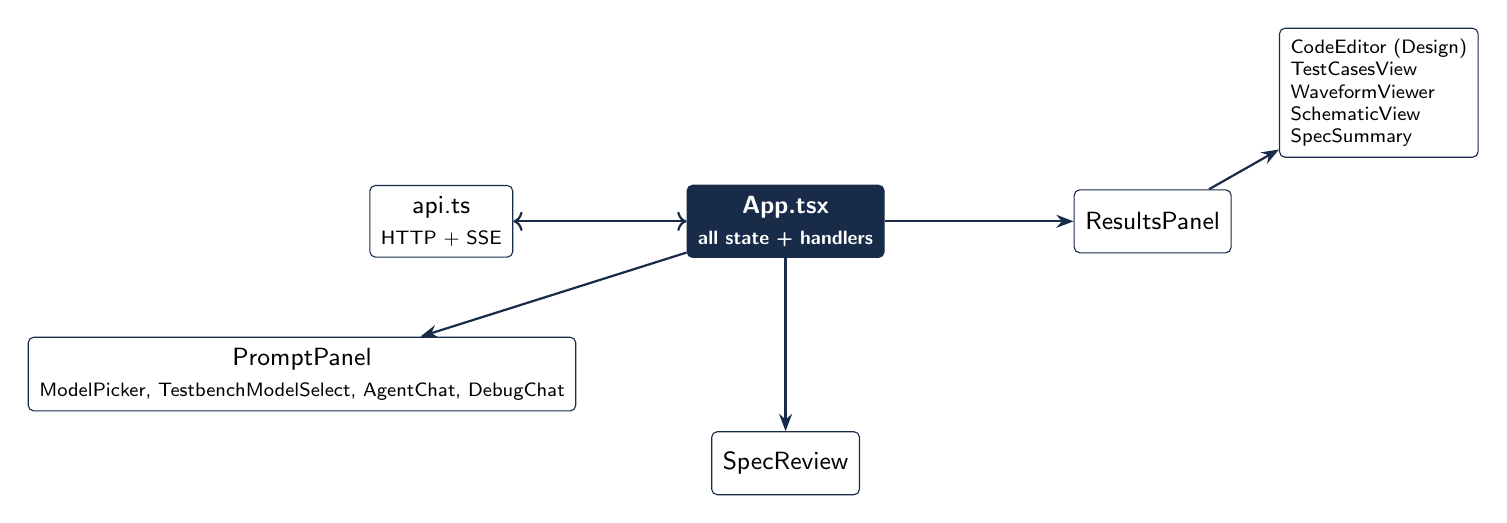
\begin{tikzpicture}[node distance=6mm and 5mm,font=\small]
  \node[hbox] (app) {App.tsx \\ \scriptsize all state + handlers};
  \node[box,below left=10mm and 14mm of app,align=center] (pp) {PromptPanel \\ \scriptsize ModelPicker, TestbenchModelSelect, AgentChat, DebugChat};
  \node[box,below=22mm of app] (spec) {SpecReview};
  \node[box,right=24mm of app] (rp) {ResultsPanel};
  \node[box,above right=4mm and 6mm of rp,align=left,font=\scriptsize] (tabs) {CodeEditor (Design) \\ TestCasesView \\ WaveformViewer \\ SchematicView \\ SpecSummary};
  \node[box,left=22mm of app] (api) {api.ts \\ \scriptsize HTTP + SSE};
  \foreach \t in {pp,spec,rp} \draw[arr] (app)--(\t);
  \draw[arr] (rp)--(tabs); \draw[arr,<->] (app)--(api);
\end{tikzpicture}}
\caption{Component tree. App owns the data; components receive it as props and report user actions back.}
\end{figure}

\section{App.tsx: state and handlers}

\code{App} keeps all state with React's \code{useState}: the provider badge, the model list and sources, the chosen model, testbench model and thinking level, the review-the-specification switch, the RTL and testbench text, module name, explanation, result, waveform, schematic, iteration history, design id, synthesis, strength, timing, second opinion, the models that wrote the design and testbench, the specification used, lint info, fallback notice and warning, timeline messages and saved projects. On first load it calls \code{getModels} (which also tells it whether the backend is live or offline) and \code{listProjects}. If the backend cannot be reached, the header shows a red ``Server not reachable'' badge with a Retry button: an unreachable server is not a mode, and the old offline-demo badge made it look like one. The chosen model, testbench model, ``Show other models'' and the review switch are remembered in the browser (\code{localStorage}).

\begin{description}
  \item[\code{loadModels}, \code{chooseModel}] Read the Model menu from \code{/api/models}; keep the current choice if it is still offered, otherwise restore the remembered one, otherwise use the server's default. A testbench model that is no longer offered is cleared.
  \item[\code{handleGenerate}] If the review switch is on (and the app is live), call \code{parseSpec} and show the SpecReview panel; otherwise call \code{startRun} straight away.
  \item[\code{startRun}] Clears \emph{every} result of the previous run, including the RTL, testbench, explanation and design id (otherwise a new run that failed after its RTL arrived left the new RTL next to the old testbench, and Re-run checked that mixed pair), closes any open specification review, opens the stream (with the confirmed specification if there is one), and for each event: adds a timeline message, shows a fallback notice once (\code{lastNoticeRef} prevents duplicates), clears old lint when a repair changes the code, and fills whichever fields the event carries. On \code{done} it loads the complete response (including \code{pass_disputed}), switches to the Results tab and refreshes Projects. It turns network problems into plain messages that say the run is lost and what to do.
  \item[\code{handleCancel}] Aborts the stream or a re-run (the Stop button). Both now carry an abort signal; Stop used to do nothing during a Re-run.
  \item[\code{handleReRun}] Sends the edited code to \code{/api/simulation/run} once, without the AI. It clears strength, synthesis, timing, second opinion, lint and ``Design written by'', because those described the previous code, and shows the note ``Re-run of edited code: only the simulation was repeated \ldots''.
  \item[\code{handleEvidenceRun}, \code{handleApplyFix}] For the debugging agent: when its evidence run simulated code that differs from the results on screen, show that run instead (with a timeline message); put a fix from the agent into the editor and open the Design tab.
  \item[\code{handleUVMExport}] Requests the bundle and downloads the zip; a second click while an export is running is ignored.
  \item[\code{handleLoadProject}, \code{handleDeleteProject}] Open or delete a saved run (deleting asks for confirmation). Loading resets the repair count and lint too, and a counter (\code{loadSeq}) makes sure only the \emph{latest} load writes the screen: two quick clicks used to let the slower, older project overwrite the newer one.
\end{description}

\section{api.ts and streaming}
\label{sec:apits}

The browser's built-in \code{EventSource} cannot send a POST body, so \code{streamDesign} uses \code{fetch} and reads the response body as a stream. It decodes chunks into a buffer, normalises \texttt{\textbackslash r\textbackslash n} to \texttt{\textbackslash n} on the whole buffer (a pair can be split across two chunks), splits on blank lines, takes the \code{data:} line of each frame and parses its JSON. After Stop, frames already received are not applied (a cancelled run used to apply its final result), and the stream is always closed, even if handling an event throws. A FastAPI validation error (a list of messages) is shown as its messages, not as raw JSON. HTTP 502/504 errors say that the server did not answer in time. \file{api.stream.test.ts} runs this real function against a fake server; every other App test replaces it with a stub.

\section{The components}

\begin{description}
  \item[PromptPanel] The sidebar: the ``Describe the block'' text box with a character count, the Generate RTL button, the run timeline (passed in as a child), four example chips (including ``Buggy counter'', scripted only in offline mode), the Model menu, ``Testbench written by'', ``Review the specification before generating'', a thinking-level selector for models that have one, and the Target clock slider (10--500 MHz). Ctrl/Cmd+Enter submits.
  \item[ModelPicker] Three source tabs (OpenCode, Cloudflare, NVIDIA NIM) with arrow-key navigation, a refresh button, the model drop-down grouped by provider (free models marked ``(free)''), the model's note, a hint when a source is not set up, and on the OpenCode tab the ``Show other models'' check box with the number hidden.
  \item[TestbenchModelSelect] ``Testbench written by'': ``Same model as the design'' or any model from any source.
  \item[SpecReview] The specification review panel: module, ports and parameters, editable behaviour and constraints, ``Generate with this specification'' and Cancel.
  \item[AgentChat] The run timeline: one message per event with an icon for its stage and status, the structured diagnosis folded under a ``Diagnosis'' line (it is also on the Results tab), with \texttt{`code`} from the model shown as code, a ``Working\ldots'' timer while a run is going, and the design explanation.
  \item[DebugChat] The ``Ask about this run'' panel under the run timeline: questions, the evidence steps, the answer with clickable times, and the fix card with the server's verdict (Chapter~\ref{ch:agent}).
  \item[CodeEditor] Two tabs (RTL and testbench) using CodeMirror with Verilog highlighting, editable, with a copy button. Edited code can be re-simulated with Re-run. It is shown on the Design tab (before any run, the Design tab shows a welcome page with recent projects instead).
  \item[ResultsPanel] Five tabs: Design, Results, Test cases, Waveform, Schematic. \emph{Results}, top to bottom: the built-in-demo tag when the result is not from an AI model, the verdict (status badge, which reads ``PASS, disputed'' in warning colour when the evidence contradicts the PASS; checks, passed, failed, pass rate), the ``Do not trust this PASS yet'' line, warnings, the second opinion, ``Design written by'', then sections for testbench strength, synthesis, timing and area (with the equivalence line, \code{EquivalenceLine}, and the fold-out critical path table, \code{CriticalPath}), toggle coverage, test types, lint, the self-correction loop, errors and the specification used (SpecSummary).
  \item[TestCasesView] Every executed check, with filters, search and a bit-by-bit comparison (Section~\ref{sec:testcases}).
  \item[WaveformViewer] Draws the waveform as SVG: a time ruler, single-bit signals as high/low lines, buses as labelled hex segments, zoom (0.5$\times$ to 4$\times$) and reset, and a notice when data was truncated. No external tool such as GTKWave is needed. Values are formatted by \code{formatValue}, which never fails: Icarus prints a partly unknown nibble in capitals (\code{X0}), and that once threw an error in decimal mode that blanked the whole page. Only a pinned cursor is announced to screen readers, and a cursor from one run is not carried to the next.
  \item[ErrorBoundary] Wraps the results panel: if any part of it fails to draw, that panel shows the error and a ``Try again'' button, and the rest of the app keeps working.
  \item[SchematicView] Three views chosen with buttons: \emph{Block diagram} (the module as a box with input ports on the left, outputs on the right and widths shown as \code{[n:0]}, drawn by the component itself), \emph{RTL cells} and \emph{Gate level} (the two netlists of Section~\ref{sec:schematicnetlists}). A view without a netlist is greyed out, with the reason as a tooltip. The netlist views are laid out by \textbf{netlistsvg} (open source, MIT licence) through \file{netlistRender.ts}, which is \emph{lazy-loaded}: the layout engine is fetched with a dynamic \code{import} only the first time such a view is opened, so the first page load stays fast. The SVG it returns is shown through an \code{<img>} tag from a blob URL, not inserted into the page: an SVG shown as an image cannot run script, whatever names the design's signals carry. Above 400 cells (\code{MAX_DRAWN_CELLS}) nothing is drawn and the tab says why. Zoom (0.5$\times$ to 6$\times$), \emph{Fit to panel} and \emph{Download SVG} work on the drawn view.
\end{description}

% ---------------------------------------------------------------------------
\chapter{The Debugging Agent}
\label{ch:agent}

Everything so far is a \emph{fixed pipeline}: the orchestrator decides which step runs next, and the model only fills in each step. This chapter describes the one part of SiliconScribe where the model decides what to look at. In the app it is the panel \textbf{Ask about this run} in the left sidebar, under the run timeline. You type a question about the code in the editor (``Why did the first check fail?''), and the answer is built from the simulation itself: values read from the waveform at exact times, lines found in the source, and fixes that the server has simulated.

It was added on 24 November 2026, \emph{after} the project report was submitted (deadline 6 November 2026). In the report it appears only as an extension after submission, never as part of the submitted work. The code is on the branch \code{agent-debug}, commit \code{3d05b94}.

\begin{center}
\small
\begin{tabularx}{\textwidth}{@{}>{\raggedright\arraybackslash}p{5.0cm}X@{}}
\toprule
\textbf{File} & \textbf{What it does} \\
\midrule
\file{backend/agent.py} & The tool loop: the system prompt, the eight tools (\code{Toolbox}), the overview, the grounding rule, fix verification and the rule-based fallback. \\
\file{backend/wave_query.py} & \code{WaveDB}: a queryable copy of one run's VCD (exact values at exact times, for any signal). \\
\file{backend/main.py} & \code{agent_ask}, the route \code{POST /api/agent/ask}: the evidence run and the event stream. \\
\file{backend/llm_service.py} & \code{agent_chat} (one model turn, plain text in and out) and \code{uses_offline}. \\
\file{frontend/src/components/}\newline\file{DebugChat.tsx} & The panel: questions, evidence steps, the answer, clickable times and the fix card. \\
\file{frontend/src/api.ts} & \code{askAgent}, which reads the stream with the same \code{readSSE} function as a normal run. \\
\bottomrule
\end{tabularx}
\end{center}

\section{What an agent is}

A plain chat model answers from the text it was given. If you paste a Verilog file and ask ``why does the hold check fail?'', it reads the code and \emph{guesses} what the hardware did. It cannot see the waveform, so it can describe a waveform that never happened (Section~\ref{sec:llmalonefails} explains why that is the core problem of using a model for hardware).

An \textbf{agent} is a model placed in a loop with \textbf{tools}. A tool is a small function on the server that does one real thing, such as ``give me the value of \code{count} at 25 ns''. In each turn the model either asks for one tool or gives its final answer. The server runs the tool, adds the result to the conversation, and asks the model again. The model chooses the questions; the server supplies the answers from real data.

\begin{analogy}
A doctor on the phone can only guess from what you say. A doctor in a clinic can order a blood test, read the result, then order the next test that result suggests. The tools are the lab tests: the doctor chooses them, but the numbers come from the lab, not from the doctor's memory.
\end{analogy}

\begin{figure}[H]
\centering
\resizebox{\textwidth}{!}{%
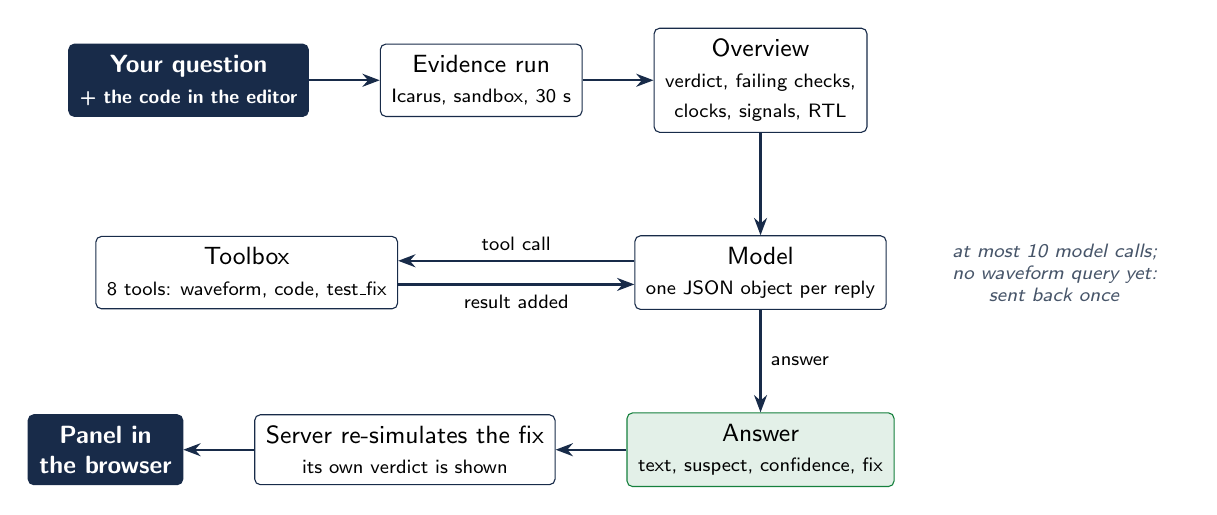
\begin{tikzpicture}[node distance=6mm and 9mm]
  \node[hbox] (q) {Your question\\ \scriptsize + the code in the editor};
  \node[box,right=of q] (sim) {Evidence run\\ \scriptsize Icarus, sandbox, 30 s};
  \node[box,right=of sim] (ov) {Overview\\ \scriptsize verdict, failing checks,\\ \scriptsize clocks, signals, RTL};
  \node[box,below=13mm of ov] (m) {Model\\ \scriptsize one JSON object per reply};
  \node[box,left=30mm of m] (tb) {Toolbox\\ \scriptsize 8 tools: waveform, code, test\_fix};
  \node[okbox,below=13mm of m] (ans) {Answer\\ \scriptsize text, suspect, confidence, fix};
  \node[box,left=of ans] (fx) {Server re-simulates the fix\\ \scriptsize its own verdict is shown};
  \node[hbox,left=of fx] (ui) {Panel in\\ the browser};
  \draw[arr] (q)--(sim); \draw[arr] (sim)--(ov); \draw[arr] (ov)--(m);
  \draw[arr] ([yshift=1.5mm]m.west) -- node[above,font=\scriptsize]{tool call} ([yshift=1.5mm]tb.east);
  \draw[arr] ([yshift=-1.5mm]tb.east) -- node[below,font=\scriptsize]{result added} ([yshift=-1.5mm]m.west);
  \draw[arr] (m)--node[right,font=\scriptsize]{answer}(ans);
  \draw[arr] (ans)--(fx); \draw[arr] (fx)--(ui);
  \node[note,right=4mm of m,text width=3.2cm] {at most 10 model calls;\\ no waveform query yet:\\ sent back once};
\end{tikzpicture}}
\caption{One question. The model chooses the tools; every tool result comes from the simulator or the source, and every fix is simulated again by the server before it is shown.}
\label{fig:agentloop}
\end{figure}

\section{The protocol: one JSON object per reply}

The system prompt (\code{SYSTEM_PROMPT} in \file{agent.py}) tells the model that every reply must be exactly one JSON object, in one of two shapes:

\begin{lstlisting}[style=plain]
{"thought": "one short sentence", "tool": "cycle_table",
 "args": {"signals": ["enable", "count"], "from_ns": 0, "to_ns": 100}}

{"answer": "<markdown>", "suspect": "design" | "testbench" | "both" | "unclear" | "none",
 "confidence": "high" | "medium" | "low",
 "fix": {"file": "rtl" | "testbench", "code": "<the COMPLETE corrected file>"}}
\end{lstlisting}

The first is a tool call, the second the final answer (\code{fix} is optional). The prompt also gives the working rules: start from the first failing check, remember that the testbench can be wrong too, test a fix before claiming it works, query the waveform at least once, and write every time as ``@125ns'' so the user can click it.

\subsection{Why plain JSON text and not native function calling}

Some AI services offer \textbf{native function calling}: the program declares its tools in a special field of the request, and the service returns a structured tool call instead of text. SiliconScribe does not use it. Its models come from four kinds of source (the OpenCode app, Cloudflare Workers AI, NVIDIA NIM and any OpenAI-compatible endpoint), and they do not all offer that field in the same way. The OpenCode app, for example, is driven through its command line (Section~\ref{sec:routing}): the prompt goes in as text and the answer comes back as text, with no place to declare tools. Plain JSON in plain text works the same through every source, so the agent works with any model in the Model menu.

The price is that the reply must be parsed. \code{_parse_reply} uses the same forgiving reader as the rest of the app (\code{_extract_json}, Section~\ref{sec:llmparse}), which takes the last complete JSON object in the reply. A reply that is not one of the two shapes counts as a \textbf{format slip}: the first time, the model is told ``Your reply was not one JSON object'' and asked again; after a second slip its text is shown, with the note ``The model did not follow the tool protocol; this text is unchecked.''

Each model turn is one call of \code{agent_chat} in \file{llm_service.py}: the chosen model, temperature 0.1, the system prompt and a transcript that holds the question, up to 4 earlier questions and answers of the conversation, the overview, and every step so far. The last 5 tool results are kept whole (up to 3000 characters each); older ones are shortened to 400 characters, because each turn sends the whole growing transcript again.

\section{The evidence run}

The question is about the code \emph{in the editor}, which may have been edited since the last run. So the first thing \code{agent_ask} in \file{main.py} does is simulate that code again, with \code{_rerun}, the same function the Re-run button uses: a fresh workspace folder (\code{new_workspace_id}), Icarus Verilog, the full sandbox policy and allow-list (Section~\ref{sec:sandbox}), the resource caps, and a 30-second limit. \code{_simulate_checked} also applies the rule that a testbench without checks can never PASS. A \code{$system} call in the code is refused here exactly as in a normal run.

The result is streamed to the browser as a \code{run} event. If the editor's code differs from the code whose results are on screen, the Results and Waveform tabs switch to this run, and the timeline says so (``The code was edited since the last run, so the question re-simulated it \ldots''). That way the times in the answer always match the waveform on screen. If the code is unchanged, nothing on screen changes: Icarus gives the same result for the same code.

\code{overview} then writes a short summary that opens the model's first turn: the verdict and counts; for ERROR or TIMEOUT the error lines and the end of the log; the first six failing checks with their times; how long the simulation ran and the length of one VCD tick; up to two clocks with their period and first rising edge; the list of signals (up to 80, the design's own first); the RTL with line numbers (up to 400 lines); and the length of the testbench (the model reads it with \code{read_code} when it needs to).

\section{WaveDB: reading a VCD for questions}
\label{sec:wavedb}

A VCD file (Section~\ref{sec:vcdbasics}) is a list of value changes in time order. The waveform viewer gets a compact copy (\code{parse_vcd}: at most 40 signals and 2000 changes each, in hex). The agent needs something else: the exact value of \emph{any} signal at \emph{any} time, without ever putting the whole file into a prompt. \code{wave_query.load} builds that copy, called a \code{WaveDB}:

\begin{enumerate}
  \item Read at most 8 MB of the file (the same cap as the viewer; if the file was larger, \code{partial} is set and the overview says late changes are missing), the timescale, and every \code{$var} declaration. Parameters, events and strings are skipped.
  \item Walk the changes. \texttt{\#t} sets the current time; \code{1!} or \code{b0101 code} is a change of one signal. Each value is stored as binary text padded to the signal's width (\code{x} and \code{z} bits are kept). A repeated dump of the same value is not a change.
  \item If a signal changes several times in one time step, only the \textbf{settled} value is kept. That is what the step ends with, and what any later code sees.
  \item Each signal ends up with two lists: the times of its changes and the values. Up to 2000 signals and 200,000 changes per signal are kept.
\end{enumerate}

Looking up a value is then a \textbf{binary search} in the list of times (Python's \code{bisect}), the way you find a word in a dictionary by opening it in the middle rather than reading from page one. \code{resolve} finds a signal by full path (\code{testbench.dut.count}), by the end of a path (\code{dut.count}) or by bare name (\code{count}); when several match, the design's own copy wins over a testbench variable of the same name.

\subsection{value\_at and value\_before: why ``just before the edge''}

Every signal has two lookups, and the difference between them is the most important idea in this chapter:
\begin{description}
  \item[\code{value_at(t)}] the value \emph{after} every change at time $t$: the last change at or before $t$.
  \item[\code{value_before(t)}] the value \emph{just before} $t$: the last change strictly before $t$.
\end{description}

Why both? Take a counter at a rising clock edge at 25 ns. In the VCD, \code{count} has a change \emph{at} 25 ns, because the flip-flops updated on that edge. But the flip-flops decided what to store from the values their inputs had \emph{just before} the edge: at the instant the clock rises, a flip-flop takes a snapshot of its input, and only then does its output change (Section~\ref{sec:seqlogic}). If the agent read \code{enable} ``at'' 25 ns, it would see the value after the edge, which may already have been changed by the testbench in the same time step. That is not what the flip-flop saw. So \code{value_before} answers ``what did the flip-flop sample?'' and \code{value_at} answers ``what did it store?''.

\begin{keyidea}
At a clock edge, read the inputs \emph{just before} the edge and the outputs \emph{after} it. A flip-flop samples before and updates after. Reading both at the same instant is the classic off-by-one-cycle mistake in waveform debugging, and it is exactly the mistake the \code{cycle_table} tool is built to avoid.
\end{keyidea}

This was checked by sabotage: making ``just before'' return the same as ``after'' (together with making the fix check always report PASS) made 4 backend tests fail.

\subsection{Times: nanoseconds and ticks}

The VCD stores times as whole \textbf{ticks} of its timescale. The model always speaks in nanoseconds. \code{to_ticks} converts with $\text{ticks} = \text{ns} \times 1000 / \text{tick length in ps}$, and \code{to_ns} converts back. In the runs shown in this guide one tick is 1 ps, so 30 ns is 30,000 ticks. \code{edges} finds rising or falling edges of a 1-bit signal; as in Verilog, a change from \code{x} or \code{z} to 1 also counts as a rising edge. \code{clocks} finds 1-bit signals named like \code{clk} or \code{clock}.

\section{The eight tools}

\code{Toolbox} in \file{agent.py} holds the run being discussed (its \code{WaveDB}, its result, the RTL and testbench) and offers eight tools. Times in the arguments are nanoseconds.

\begin{center}
\small
\begin{tabularx}{\textwidth}{@{}>{\ttfamily}lX@{}}
\toprule
\textrm{\textbf{Tool}} & \textbf{What it returns} \\
\midrule
failing\_checks & The testbench's failed comparisons: number, time, type, name, expected and actual value (up to 25 per call, with an offset to page through more). \\
values\_at & Each signal's value at a time \emph{and} just before it (``\code{count = 4'h2 (2) (was 4'h1 (1))}''). Without a signal list it reads the design's ports. Up to 12 signals per call. \\
changes & Every change of one signal in a time window, and the value entering the window (at most 40 changes; it says when there are more). \\
cycle\_table & One row per clock edge: each signal's value sampled just \emph{before} the edge (what the flip-flops see) and \emph{after} it. Up to 32 rows. The best tool for sequential logic. The clock is found by name when there is one. \\
find\_value & When a signal held a given value, written in decimal (\code{9}), hex (\code{4'h9}, \code{0x9}), binary (\code{4'b1001}), \code{x} or \code{z} (up to 5 intervals). \\
drivers & Source lines that assign a signal (left side of \code{=} or \code{<=}, not a \code{==} comparison), with the enclosing \code{always} or \code{assign} block, plus instance ports connected to it. This is a \emph{text search} with comments and strings blanked, not a full elaboration of the design, and it says so. \\
read\_code & Numbered lines of the RTL or the testbench (at most 120 per call). \\
test\_fix & Simulates a candidate fix (the complete corrected file) with the other file unchanged, and returns the verdict and the first failing checks. At most 3 per question. \\
\bottomrule
\end{tabularx}
\end{center}

Values are written as \code{4'h9 (9)}: hex always, decimal too when no bit is \code{x} or \code{z} (\code{fmt_value}). A bad call (an unknown signal, a missing time, a fourth \code{test_fix}) raises \code{ToolError}; its message goes back to the model as the tool result, with hints such as similar signal names, so the model can correct itself. A crash inside a tool is logged and reported as ``Tool error'' without ending the conversation. A tool result is cut at 3000 characters. For \code{test_fix}, the code argument is replaced by ``\textless N characters\textgreater'' in the events sent to the browser, so a long file is not echoed back.

\section{The grounding rule}

An answer about a run must rest on the run. The four waveform tools and \code{test_fix} are the tools that read the simulation (\code{WAVE_TOOLS}). If the model answers before any of them has given a real result (a call that ended in a tool error does not count), the answer is not shown. Instead the model is told once: ``Before answering, confirm your explanation with at least one waveform query \ldots, then answer.'' If it answers again without one, that second answer is accepted, so a stubborn model cannot loop forever. A run with no waveform at all (it did not compile) is exempt.

The rule came from a live result. With the model \code{opencode/deepseek-v4.1-flash-free}, the hidden counter bug (A4 in Table~\ref{tab:agentlive}) was diagnosed correctly and the fix passed 57/57, but with \emph{zero} tool calls: the model reasoned from the overview alone. It was right that time, but nothing in the answer came from the waveform.

\section{The answer and the fix}

The final answer carries markdown text, a \textbf{suspect} (design, testbench, both, unclear or none) and a \textbf{confidence} (high, medium or low); anything else is replaced by ``unclear'' or ``medium''. If it includes a fix, \code{_verified_fix} decides what happens to it:
\begin{enumerate}
  \item It must name the RTL or the testbench, contain a module and be at most 50,000 characters; otherwise it is dropped.
  \item A ``fix'' identical to the current file is dropped.
  \item The server simulates it (\code{run_fix}, in the same sandbox, other file unchanged). If the model already tested exactly this code with \code{test_fix}, that result is reused, since the same code gives the same verdict.
  \item The answer carries \emph{that} verdict: status and counts, for example ``PASS, 57 of 57 checks''. If the fix cannot even be simulated, it is shown as ERROR with the reason, not hidden.
\end{enumerate}
The model's own claim that the fix works is never shown as the verdict. A testbench fix also gets a warning in the panel: ``This changes the checker itself. A testbench fix can make a wrong design pass: read it before you apply it.''

\begin{warnbox}[What is checked and what is not]
Only the \emph{fix} is checked, by simulation. The \emph{explanation} is model text and is not verified. In one live run (A6 below) the fix passed 558 of 558 checks, but the explanation was only partly right. A passing fix proves that the new code passes this testbench, not that the model understood why the old code failed.
\end{warnbox}

\section{When there is no AI: rule-based evidence}

\code{rule_based_answer} collects the same kind of evidence with fixed rules: the verdict, the first failing check (name, time, expected and actual), the values of the ports at that time, a cycle table of the edges before it, and the lines that assign the design's outputs. It is used in three cases:
\begin{itemize}
  \item no AI model is connected (\code{uses_offline} says the chosen model would be served by the offline demo provider);
  \item the model call fails: a usage limit, a timeout or another provider error (the reason is named);
  \item the model used all 10 steps without answering (from step 8 on, the transcript asks it to answer now).
\end{itemize}
The text starts with the reason in bold and ``This is evidence collected by fixed rules, not an AI diagnosis'', and the panel labels it \textbf{Rule-based evidence (no AI)}. It is never presented as the AI's answer: there is no silent swap. This follows the same honesty rule as the main pipeline's fallback (Section~\ref{sec:fallback}).

\section{The event stream}

\code{POST /api/agent/ask} answers with Server-Sent Events, like a normal run, but each event has a \code{type} field instead of \code{stage}:

\begin{center}
\small
\begin{tabularx}{\textwidth}{@{}>{\ttfamily}lX@{}}
\toprule
\textrm{\textbf{type}} & \textbf{Meaning and fields} \\
\midrule
status & Progress text: ``Simulating the code in the editor to collect evidence\ldots''. \\
run & The evidence run: \code{result}, the full simulation result with its waveform. \\
tool & One tool call: \code{tool}, \code{args}, the model's \code{thought}, \code{ok} (false for a tool error), a one-line \code{summary} and the \code{result} text. \\
answer & The end: \code{text}, \code{suspect}, \code{confidence}, \code{fix} (with the server's verdict, or null), \code{rule_based}, \code{steps}, the \code{model} (null for rule-based), and \code{note} when the text is unchecked. \\
error & The end, when something failed: a short, safe \code{message}. \\
\bottomrule
\end{tabularx}
\end{center}

Exactly one \code{answer} or \code{error} ends every stream. The request is checked by Pydantic (\code{AgentRequest}): RTL and testbench of 1 to 50,000 characters each, a question of 1 to 2000 characters, at most 6 earlier turns, a model id that matches the safe pattern (Section~\ref{sec:modelid}), and an optional thinking level. The rate limit applies, as on every other route.

\section{The panel in the browser}

\code{DebugChat} is shown in the sidebar once there is an RTL and a testbench. It is disabled while a generation or a Re-run is in progress, and a new design starts a fresh conversation. Its parts:
\begin{description}
  \item[Asking] Three example questions (``Why did the first check fail?'', ``Is the design or the testbench wrong?'', ``Walk me through the first 5 clock cycles.''), or your own question (Enter sends, Shift+Enter adds a line). \code{ask} sends the code exactly as it is at that moment, the chosen model and thinking level, and up to 4 earlier questions and answers. \textbf{Stop} aborts the request.
  \item[Evidence steps] Each \code{tool} event becomes one numbered step with a plain label (``Built a cycle-by-cycle table: enable, count 0--100ns''). Click a step to see the model's thought and the raw tool result. A failed tool call is marked.
  \item[The answer] A header that says \textbf{AI answer} with the number of evidence steps, or \textbf{Rule-based evidence (no AI)}; the model id; ``Suspect: Design \textbullet\ confidence high'' (hidden when unclear); the note, if any; then the text.
  \item[Plain text only] \code{RichText} shows the model's text as plain text. Only three things are recognised: \texttt{`code`}, \texttt{**bold**} and times. Nothing is ever inserted as HTML, so a model cannot put a script or a fake button into the page.
  \item[Clickable times] A time such as ``@30ns'' or ``30 ns'' becomes a button. The waveform viewer works in VCD ticks, so \code{inline} converts: $\text{ticks} = \text{round}(\text{ns} \times 1000 / \text{timescale\_ps})$. Clicking it opens the Waveform tab with cursor A at that time. A sabotage test proved this matters: a wrong ns-to-tick conversion made a frontend test fail.
  \item[The fix card] Green for PASS, red otherwise: ``Proposed fix to the design: the server re-simulated it, PASS (57 of 57 checks passed)'', the testbench warning when the fix is to the testbench, the failing checks when it did not pass, a fold-out with the proposed code, and \textbf{Apply to the editor}. Applying puts the code in the editor and opens the Design tab; the main results change only when you press \textbf{Re-run}.
\end{description}

When the \code{run} event arrives, \code{handleEvidenceRun} in \file{App.tsx} compares the code that was asked about with the code whose results are on screen; if they differ, the evidence run replaces the results, exactly as a Re-run would (\code{applyRerun}). \code{askAgent} reads the stream with the same \code{readSSE} function as \code{streamDesign} (Section~\ref{sec:apits}), treats \code{answer} and \code{error} as final, and says ``The connection closed before the answer arrived'' if neither came.

\section{A worked example: the hidden counter bug}
\label{sec:agentexample}

The built-in 4-bit counter (Section~\ref{sec:counterexample}) was given a bug with no comment pointing at it: \code{else if (enable)} became \code{else if (enable || count[0])}. Whenever the lowest bit is 1, the counter now counts even with \code{enable} low. The testbench is unchanged; its hold checks set \code{enable} to 0 and expect \code{count} to stay put. The simulator says FAIL, 12 of 57 checks passed (45 failed).

On 24 November the question was asked live with the model \code{nvidia/nemotron-3-ultra-550b-a55b} on NVIDIA NIM (A2 in Table~\ref{tab:agentlive}). The answer took 34 s. The model built a cycle table, which showed \code{count} changing while \code{enable} was 0, at 25, 55 and 85 ns. This is what that table looks like (reproduced afterwards by running the same tool on the same code; the rows from 15 to 55 ns):

\begin{lstlisting}[style=plain]
posedge of testbench.clk; 'before' = sampled by flip-flops at the edge, 'after' = value once
the edge's updates settled.
cycle | time | enable before -> after | count before -> after
    1 | 15ns | 1                      | 4'h0 (0) -> 4'h1 (1)
    2 | 25ns | 0                      | 4'h1 (1) -> 4'h2 (2)     <- enable was 0, count moved
    3 | 35ns | 0                      | 4'h2 (2)                 <- count[0] is 0: it holds
    4 | 45ns | 1                      | 4'h2 (2) -> 4'h3 (3)
    5 | 55ns | 0                      | 4'h3 (3) -> 4'h4 (4)     <- moved again
\end{lstlisting}

Read row 2 with the key idea above: just before the edge at 25 ns, \code{enable} was 0 and \code{count} was 1; after it, \code{count} was 2. A correct counter must hold there. Row 3 is the clue to the cause: with \code{count} = 2 (lowest bit 0) it does hold. So the counter moves only when the lowest bit is 1, which points straight at \code{count[0]} in the condition. The testbench's first hold check, at 30 ns, expected 1 and got 2.

The answer correctly blamed the condition in the design, and its proposed fix was re-simulated by the server: \textbf{PASS, 57 of 57}. Figures~\ref{fig:askpanel} and~\ref{fig:askjump} in Chapter~\ref{ch:usage} show the same bug asked in the real browser (A3).

\section{Live results}

These are single runs on small designs, mainly with one model, on 24 November 2026: evidence that the mechanism works, not a benchmark. The model is \code{nvidia/nemotron-3-ultra-550b-a55b} on NVIDIA NIM unless stated.

\begin{center}
\small
\begin{longtable}{@{}l>{\raggedright\arraybackslash}p{3.9cm}>{\raggedright\arraybackslash}p{6.1cm}>{\raggedleft\arraybackslash}p{2.2cm}@{}}
\caption{Live results of the debugging agent.}\label{tab:agentlive}\\
\toprule
\textbf{\#} & \textbf{Case} & \textbf{Result} & \textbf{Time} \\ \midrule \endfirsthead
\toprule
\textbf{\#} & \textbf{Case} & \textbf{Result} & \textbf{Time} \\ \midrule \endhead
A1 & Built-in buggy counter (adds 2; the RTL has a ``BUG'' comment) & Correct, design; fix re-simulated 57/57 & 31 s \\
A2 & Hidden bug \code{enable || count[0]}, no comment & Correct; used a cycle table (count moves while enable = 0 at 25, 55, 85 ns); fix 57/57 & 34 s \\
A3 & Same hidden bug, in the real browser (twice) & Correct both times, fix 57/57; one answer cited 9 clickable times & 107 s, 74 s \\
A4 & Same hidden bug, model \file{opencode/deepseek-v4.1-flash-free} & Correct, fix 57/57, but zero tool calls (reasoned from the overview): led to the grounding rule & 49 s \\
A5 & Correct counter, wrong testbench (expects 3 instead of 2 in \code{counting_continues}) & Suspect \textbf{testbench}: the check runs at the falling edge at 560 ns, before the third rising edge; testbench fix 57/57 & 219 s, 5 steps \\
A6 & Saved SR-latch project that timed out (a real AI design from 20 Nov), real browser & Fix (gate delays) re-simulated 558/558, but the explanation was only partly right: it blamed the hold state; the real cause is the testbench releasing both inputs from 0,0 at once (Section~\ref{sec:latch-timeout}) & 316 s \\
A7 & Older saved counter whose 20-check testbench never drops enable, with the hidden bug & Said the run passed and no hold check failed (the question's premise was false) instead of inventing a failure; this weak testbench does not expose the bug & about 170 s \\
\bottomrule
\end{longtable}
\end{center}

Three of these teach the most. \textbf{A5}: the agent can say ``your design is fine, the checker is wrong'', with evidence (the time of the check relative to the clock edges). \textbf{A6}: the fix is verified, the explanation is not. \textbf{A7}: when the question assumes something false, the evidence lets the model say so.

\begin{warnbox}[Limitations]
\begin{itemize}
  \item The explanation is model text; only fixes are verified by simulation (A6).
  \item It is slow: about 30 s to 5 minutes per question on free models, because each step sends the growing transcript again.
  \item \code{drivers} is a text search, not an elaborated netlist. Icarus only: no SVA, no UVM.
  \item One run per case, small designs, mainly one model: not a benchmark.
  \item The evidence run is limited to 30 s, so a design that hangs (A6) costs the full 30 s before the model even starts.
\end{itemize}
\end{warnbox}

\begin{keyidea}
The agent does not weaken ``only the simulator decides''. The model now chooses \emph{which} questions to ask, but every answer to those questions comes from the simulator's waveform or the source text, and every fix is simulated again by the server. What the model adds is the reasoning that connects the evidence, and that part is labelled as model text.
\end{keyidea}

\begin{viva}
\emph{``Isn't this just ChatGPT with your code pasted in?''} No. A chat model guesses what the waveform looked like. Here the model must ask for the waveform: values at exact times, a table of every clock edge with the inputs sampled just before the edge, the lines that drive a signal. An answer without at least one simulation query is sent back once. And a proposed fix is never shown with the model's claim; the server simulates it and shows its own verdict.
\end{viva}

% ---------------------------------------------------------------------------
\chapter{Lessons from the Nine-Role Review}
\label{ch:review}

Before the viva the whole tool (not the documents) was reviewed once more, this time by nine reviewers, each acting as one kind of engineer. Each role looks at the same code with different questions, so each finds different defects. This chapter explains what each role looks for, the most instructive thing it found, \emph{why} the defect existed, and why the fix works. It is the best preparation for the question ``how do you know it works?''.

\section{How the review was run}

\begin{enumerate}
  \item \textbf{Nine roles, read-only.} ASIC design, design verification, backend systems, security, LLM integration, frontend, interface design, test engineering and release engineering. Each reviewer could read everything and run experiments in a scratch copy, but could not change the project. About 110 findings were reported.
  \item \textbf{Reproduce first.} No finding was fixed on someone's word. Each was reproduced with a real run (a real simulation, a real Yosys or OpenSTA run, a real browser state in a test) before any code changed.
  \item \textbf{A test for every fix.} Each fix comes with a regression test that fails without it.
  \item \textbf{Sabotage the fixes.} Each fix was then undone on purpose, one at a time, to confirm that a test fails. Four fixes survived this at first: their tests passed for the wrong reason and were rewritten.
  \item \textbf{An independent verifier.} A tenth reviewer received only the original findings and the change set (not the author's explanations), tried to break every security and verdict fix, and re-ran all saved runs with the old and new code. It found a sandbox bypass through a macro argument, a regular-expression slowdown introduced by the fixes, and three regressions. Those went through the same steps.
\end{enumerate}

\begin{keyidea}
Fixing is the easy part. The discipline is in the steps around it: reproduce the defect, pin it with a test that fails, prove the test can fail by undoing the fix, and let someone who did not write the fix try to break it. The independent round showed why: three of the author's own fixes had introduced new bugs.
\end{keyidea}

\section{What each role looks for, and what it found}

\subsection*{ASIC design engineer: ``are the numbers physically right?''}
An ASIC engineer distrusts any number until it is traced to the tool output. Here: Yosys writes large areas as \code{1.6E+03}, and the parser read only plain decimals, so a 64-bit register ``mapped to no logic''. Input and output delays were attached to the first clock only, so a slow path on a second clock was reported as meeting 500 MHz. The maximum frequency was computed with a whole-period formula even for half-cycle paths. And the equivalence proof's induction assumes all flip-flops tick together and start equal, so it ``proved'' a netlist with a flip-flop on the wrong clock edge and a design that relied on a power-up value. \emph{Lesson:} every formula has a domain where it is valid; report ``not proven'' outside it.

\subsection*{Design-verification engineer: ``can a wrong design be called PASS?''}
A verification engineer attacks the oracle and the verdict. Found: a later \code{Failed: 0} cancelled an earlier \code{Failed: 4}; \code{CHK|FAIL} rows were ignored; a design could forge the summary from a \code{final} block; the standard check compared only 64 bits; a slow testbench scored 100\% strength because timeouts counted as catches; and a repair could keep the bug and edit the expected values, leaving a green PASS that its own original testbench contradicted. \emph{Lesson:} any evidence against a PASS must win, and must be visible in the headline, not only in a warning paragraph.

\subsection*{Backend systems engineer: ``what happens under concurrency and failure?''}
Found: two runs of the same design shared one folder and swapped verdicts (25 of 25 tries); a compile timeout killed \code{iverilog} but left its child \code{ivl} spinning at 100\% CPU; a runaway testbench made the parser hold every check line in memory (about 470 MB); an old waveform was shown for a new run. \emph{Lesson:} a subprocess is a tree, a folder is shared state, and anything you read must be bounded.

\subsection*{Security engineer: ``can untrusted code reach outside its box?''}
Found: a comment between \code{$dumpfile} and its argument slipped past the path check and Icarus wrote the waveform to any path. Later the verifier found that a macro argument could deliver the \code{$} of \code{$fopen}. Also, the OpenCode child process received every API key in the environment. \emph{Lesson:} check what the tool will \emph{actually} see, which is why the rules now run on the macro-expanded source from Icarus' own preprocessor, and give child processes an allowlist, not a denylist.

\subsection*{LLM integration engineer: ``what does the app do with a bad reply?''}
Found: a Cloudflare model you chose was silently replaced by the demo when the default provider was missing; a quota error at the repair step threw away the whole run; a draft followed by a corrected module produced the module twice; reasoning text was parsed as the answer; error reasons were guessed from substrings (``token'' in \code{max_tokens} read as a credentials problem). \emph{Lesson:} assume replies are messy and services fail mid-run, keep the user's work, and give the real reason.

\subsection*{Frontend engineer: ``can the screen show something false or break?''}
Found: one unusual value (\code{X0}) in decimal mode blanked the whole page; a slow project load overwrote a newer one; Stop did nothing during a Re-run; a new run that failed early left new RTL next to the old testbench, and Re-run checked that mixed pair. \emph{Lesson:} every async result needs an identity, and one broken panel must not take down the app.

\subsection*{Interface designer: ``what will an examiner believe from the screen?''}
Found: the green PASS was louder than the caution that qualified it; saved demo runs reopened looking live; nothing said a live run takes minutes; browser zoom on a laptop projector switched to a stacked layout; the welcome text claimed more than the app proves. \emph{Lesson:} honesty is also visual hierarchy: the most important caveat must sit next to the verdict.

\subsection*{Test engineer: ``would the tests catch a regression?''}
Found by changing one line at a time: the real streaming client had no test (every App test used a stub), the anti-cheat and oscillation tests passed even with those guards removed, the admin endpoint and project deletion had no tests (a change that deleted every project passed the suite), and simply collecting the tests ran the clean-up on the real workspace. \emph{Lesson:} a test you have never seen fail is not yet a test.

\subsection*{Release engineer: ``will the demo run on the day?''}
Found: the backend listened on every network interface without a login; \code{.env.example} had active lines that override the command line; Vite silently moved to another port when 5173 was busy, leaving an old build on the expected address; preflight called a backend left in offline mode ``responding''. \emph{Lesson:} check what is actually running, not that something answers.

\section{After the review: a latch that stopped time}
\label{sec:latch-timeout}

A live run on 20 November, after the review, showed a gap that none of the nine roles had found. The prompt was simply ``design sr latch''. The run ended in \textbf{TIMEOUT} with ``0 checks, 0\%'', which looked like total failure. In fact:
\begin{enumerate}
  \item The model's first RTL used cross-coupled NOR gates, although its own truth table (active-low inputs: hold at 1,1; set at 0,1; reset at 1,0) needs NAND gates. The repair loop diagnosed this correctly and switched to \code{q = ~(s_n & q_n)}, \code{q_n = ~(r_n & q)}, the textbook latch.
  \item The repaired design then passed all 552 checks the testbench printed. After the last one, the testbench drove the forbidden input $s\_n = r\_n = 0$ (both outputs become 1) and released \emph{both} inputs to 1 in the same time step.
  \item In a real chip one gate would be slightly faster and the latch would settle (possibly after a metastable moment). A simulator without gate delays has no ``slightly faster'': both NANDs see 1,1 and switch to 0 together, then both see 0 and switch back to 1, forever. Every switch is a new \emph{delta cycle} at the \emph{same} simulated time, so time never advances.
  \item The testbench's watchdog (\texttt{\#20000; \$finish;}) waits for simulated time, so it never fired. Only SiliconScribe's 30-second wall-clock limit stopped the run.
\end{enumerate}

The verdict was right (the run never finished, so it is not a PASS), but the screen hid the evidence. Three fixes followed, each pinned by a test that fails when the fix is removed:
\begin{itemize}
  \item \textbf{The checks that ran are kept.} On a timeout the simulator now sends \code{SIGTERM} first and gives \code{vvp} two seconds to exit; \code{vvp} flushes its output on \code{SIGTERM}, whereas the old \code{SIGKILL} lost the last few kilobytes (466 of 553 lines survived). The result stays TIMEOUT with no verdict counts, but the header reads ``Checks before stop: 552'', the pass rate is shown as ``---'' (not ``0\%''), and the Test cases tab lists the checks as progress, not a verdict.
  \item \textbf{The likely cause is stated.} The timeout message now says that no watchdog fired, that simulated time therefore stopped or the run needs far longer, and that the usual cause of stopped time is a zero-delay feedback loop (cross-coupled gates, an \code{assign} that feeds itself, an \code{always} block that retriggers itself). The repair model reads the same text, and the testbench prompt now says: leave a forbidden input state one input at a time.
  \item \textbf{A stale explanation is labelled.} The model writes its explanation for the first draft, and repairs do not rewrite it, so the Run panel still described NOR gates. When a repair has changed the code, a note now says the explanation was written for the first draft.
\end{itemize}

\emph{Lesson:} a verdict can be correct and still mislead if the evidence behind it is thrown away. ``0 checks'' and ``552 checks, then the simulator stalled'' are both TIMEOUT, but only the second tells you what to fix.

\begin{viva}
\emph{``Why did the SR latch time out if the design was correct?''} Because the testbench released the forbidden 0,0 input on both pins in the same time step. With zero gate delay the two NAND gates switch together forever in delta cycles, so simulated time stops, and a \texttt{\#delay} watchdog cannot fire; only the wall-clock limit ends the run. Real hardware would settle because one gate is always slightly faster. The fix belongs in the testbench: release one input at a time.
\end{viva}

\section{Numbers to remember}

\begin{center}
\begin{tabularx}{\textwidth}{@{}X>{\raggedleft\arraybackslash}p{5.2cm}@{}}
\toprule
Findings reported by the nine roles & about 110 \\
Each fix pinned by a test that fails without it & yes (sabotage-checked) \\
Defects found by the independent verifier in the fixes & 1 bypass, 1 slowdown, 3 regressions \\
Saved runs with identical verdicts, old vs new code & 123 of 123 (and 14 of 14 evaluation designs) \\
Automated tests after the review & 591 backend + 267 frontend \\
\quad (after the debugging agent, 24 Nov) & 632 backend + 277 frontend \\
\bottomrule
\end{tabularx}
\end{center}

\begin{viva}
\emph{``Did you test your own tool, or only trust it?''} It was reviewed by nine role-based reviewers; every finding was reproduced with a real run, fixed, and pinned by a test that was shown to fail when the fix is removed; then an independent reviewer tried to break the fixes and found three regressions and a bypass, which were fixed the same way. The 123 saved runs give the same verdicts with the old and new code, so the fixes did not change any honest result.
\end{viva}


\part{Using, Testing and Extending}
% ============================================================================
%  PART III: Using, testing and extending
% ============================================================================

\chapter{Installing and Running}
\label{ch:running}

\section{What you need}

\begin{itemize}
  \item \textbf{Python 3.10+} for the backend (developed on 3.14; the Docker image uses 3.12).
  \item \textbf{Node.js 20+} and npm for the frontend.
  \item \textbf{Icarus Verilog 12} (\code{iverilog} and \code{vvp}) on the PATH. On macOS: \code{brew install icarus-verilog}; on Ubuntu: \code{sudo apt install iverilog}.
  \item For live models: the \textbf{OpenCode app}, installed and signed in with your own account. Optionally a Cloudflare account and an NVIDIA NIM key (Section~\ref{sec:providers}). Without any of these, the app runs in offline demo mode.
  \item For the timing and area estimate (optional): \textbf{Yosys} (the WebAssembly build from \code{yowasp-yosys}, reached through a \code{yosys} shim in \file{~/.local/bin}), \textbf{OpenSTA} built with \file{backend/tools/build_opensta.sh} (reached as \code{sta}), and the sky130 library file. Without them the result simply has no timing section.
  \item Optional: Verilator (better linting).
\end{itemize}

\section{First-time setup}

\begin{lstlisting}[style=plain]
cd ai-eda-playground/backend
python3 -m venv venv
source venv/bin/activate
pip install -r requirements.txt

# the sky130 cell library for timing (12 MB, not in git)
cd pdk
curl -fsSL -o sky130hd_tt.lib.gz https://raw.githubusercontent.com/parallaxsw/OpenSTA/master/examples/sky130hd_tt.lib.gz
gunzip -kf sky130hd_tt.lib.gz

cd ../../frontend
npm install
\end{lstlisting}

\section{Starting the app}

The live set-up uses two terminals. Terminal 1 starts the backend with the OpenCode app as the model provider; terminal 2 starts the frontend. The \code{PATH} addition makes \code{yosys}, \code{sta} and Icarus in \file{~/.local/bin} visible; \code{env -u OFFLINE_MODE} makes sure an old offline setting is not inherited.

\begin{lstlisting}[style=plain]
# terminal 1: backend, live model
cd ai-eda-playground/backend
PATH="$HOME/.local/bin:$PATH" env -u OFFLINE_MODE LLM_PROVIDER=opencode-app \
  LLM_MODEL=deepseek-v4.1-flash-free LLM_TIMEOUT_SECONDS=360 \
  python3 -m uvicorn main:app --host 127.0.0.1 --port 8000

# terminal 2: frontend
cd ai-eda-playground/frontend && npm run dev -- --host 127.0.0.1 --port 5173
\end{lstlisting}

Open \url{http://127.0.0.1:5173}. The badge at the top left must say \textbf{Live} followed by a model name (for example \texttt{Live \textbullet\ opencode/deepseek-v4.1-flash-free}); it follows the model chosen in the Model menu. If it says \emph{Offline demo} or \emph{Demo fallback}, the live model is not in use. During development Vite forwards \code{/api} calls to port 8000.

From the project folder, \code{./run.sh} still starts both halves in one terminal (backend on port 8000, frontend on 5173; Ctrl-C stops both), using whatever is in \file{backend/.env}.

\section{Offline mode and live mode}

\begin{description}
  \item[Offline] Set \code{OFFLINE_MODE=1} (or configure nothing). The five built-in designs are used; everything else (simulation, waveforms, repair loop, strength, timing, projects) works for real. The badge shows ``Offline demo'' and the Model menu says ``Offline demo: scripted designs, no AI model.'' The ``Buggy counter'' example is scripted only here: it shows a failure and a repair.
  \item[Live] \code{LLM_PROVIDER=opencode-app} with a default \code{LLM_MODEL}, as above. The default is only where the Model menu starts: any model can be picked per run. Free models are slow: a live run took 3 to 13 minutes in the evaluation (median 360 s), so a generous \code{LLM_TIMEOUT_SECONDS} helps.
\end{description}

\section{Optional providers: Cloudflare, NVIDIA NIM and GitHub Copilot}
\label{sec:providers}

The Model menu has three tabs. OpenCode works as soon as the app is signed in. The other two need a key, and keys go in exactly one place: the file \file{backend/.env}.

\begin{lstlisting}[style=plain]
# backend/.env  (git-ignored; keep it owner-only:  chmod 600 backend/.env)
CLOUDFLARE_ACCOUNT_ID=your_32_character_account_id
CLOUDFLARE_API_TOKEN=your_workers_ai_token
NVIDIA_NIM_API_KEY=nvapi-your_key_here
\end{lstlisting}

\begin{description}
  \item[Cloudflare Workers AI] Needs your account id (32 hexadecimal characters) and an API token with the ``Workers AI'' permission. The free plan gives 10,000 ``neurons'' a day. Some models are refused on the free plan (HTTP 403, code 5035, seen for GLM-5.3-flash and DeepSeek V4.1 Flash).
  \item[NVIDIA NIM] Needs a key that starts with \code{nvapi-}. Only \code{NVIDIA_NIM_API_KEY} is read for this tab; an older \code{NVIDIA_API_KEY} is never used for it. The fastest chat models answered in about 1 to 7 seconds; some free-queue models took 1 to 5 minutes.
  \item[GitHub Copilot] Is not configured in SiliconScribe at all. Connect it inside the OpenCode app: start \code{opencode} in a terminal, type \code{/connect}, choose GitHub Copilot and sign in with GitHub in the browser. Then press the refresh button next to the source tabs in SiliconScribe. It appears on the OpenCode tab as \code{github-copilot/auto}; because its name is not marked free, tick ``Show other models'' to see it. On the student plan only ``auto'' exists: GitHub picks the model and does not say which, so the result cannot name its model.
\end{description}

Restart the backend after editing \file{.env}. Without the keys, the Cloudflare and NVIDIA NIM tabs say they are not set up and how to fix it; nothing else changes. Delete the lines (or the file) to switch them off.

\begin{warnbox}[Keys: one place only]
Never paste a key into the web page, a prompt, a chat, a screenshot, a document or a commit. The web page never asks for one. Never commit \file{backend/.env}: it is listed in \file{.gitignore}, and the project was scanned to check that no secret is in git, in the built frontend or in the logs. The simulator, synthesis and timing tools receive a scrubbed environment, so the keys never reach them either.
\end{warnbox}

\section{Docker and deployment}

\begin{itemize}
  \item \code{docker compose up --build} builds one image (frontend compiled into \file{static/}, backend with Icarus and Yosys installed) and serves everything on port 8000, offline by default.
  \item The earlier public deployment split the halves: the frontend on Vercel (\file{vercel.json} forwards \code{/api/*} to the backend) and the backend container on Render's free plan (\file{render.yaml}, health check on \code{/health}, \code{TRUST_PROXY_HEADERS=1}). The free backend sleeps after 15 minutes idle, so the first request can take 30--50 seconds. Note that the backend now accepts browser calls only from local addresses unless the exact frontend address is added with \code{CORS_ALLOW_ORIGINS}, and the OpenCode app provider is a single-user, local convenience that must not be exposed on a public server.
\end{itemize}

% ---------------------------------------------------------------------------
\chapter{Using the Application}
\label{ch:usage}

\section{The screen}

The page has three parts. The \textbf{top bar} has the badge on the left (``Live'' with the model chosen in the menu, ``Offline demo'' or ``Demo fallback''), and on the right the \textbf{Projects} menu, \textbf{Export UVM}, \textbf{Re-run} (or \textbf{Stop} during a run) and the theme button. The \textbf{sidebar} on the left is where you describe the block, watch the run and choose settings. The \textbf{main pane} has five tabs: \textbf{Design}, \textbf{Results}, \textbf{Test cases}, \textbf{Waveform} and \textbf{Schematic}.

\begin{figure}[H]
\centering
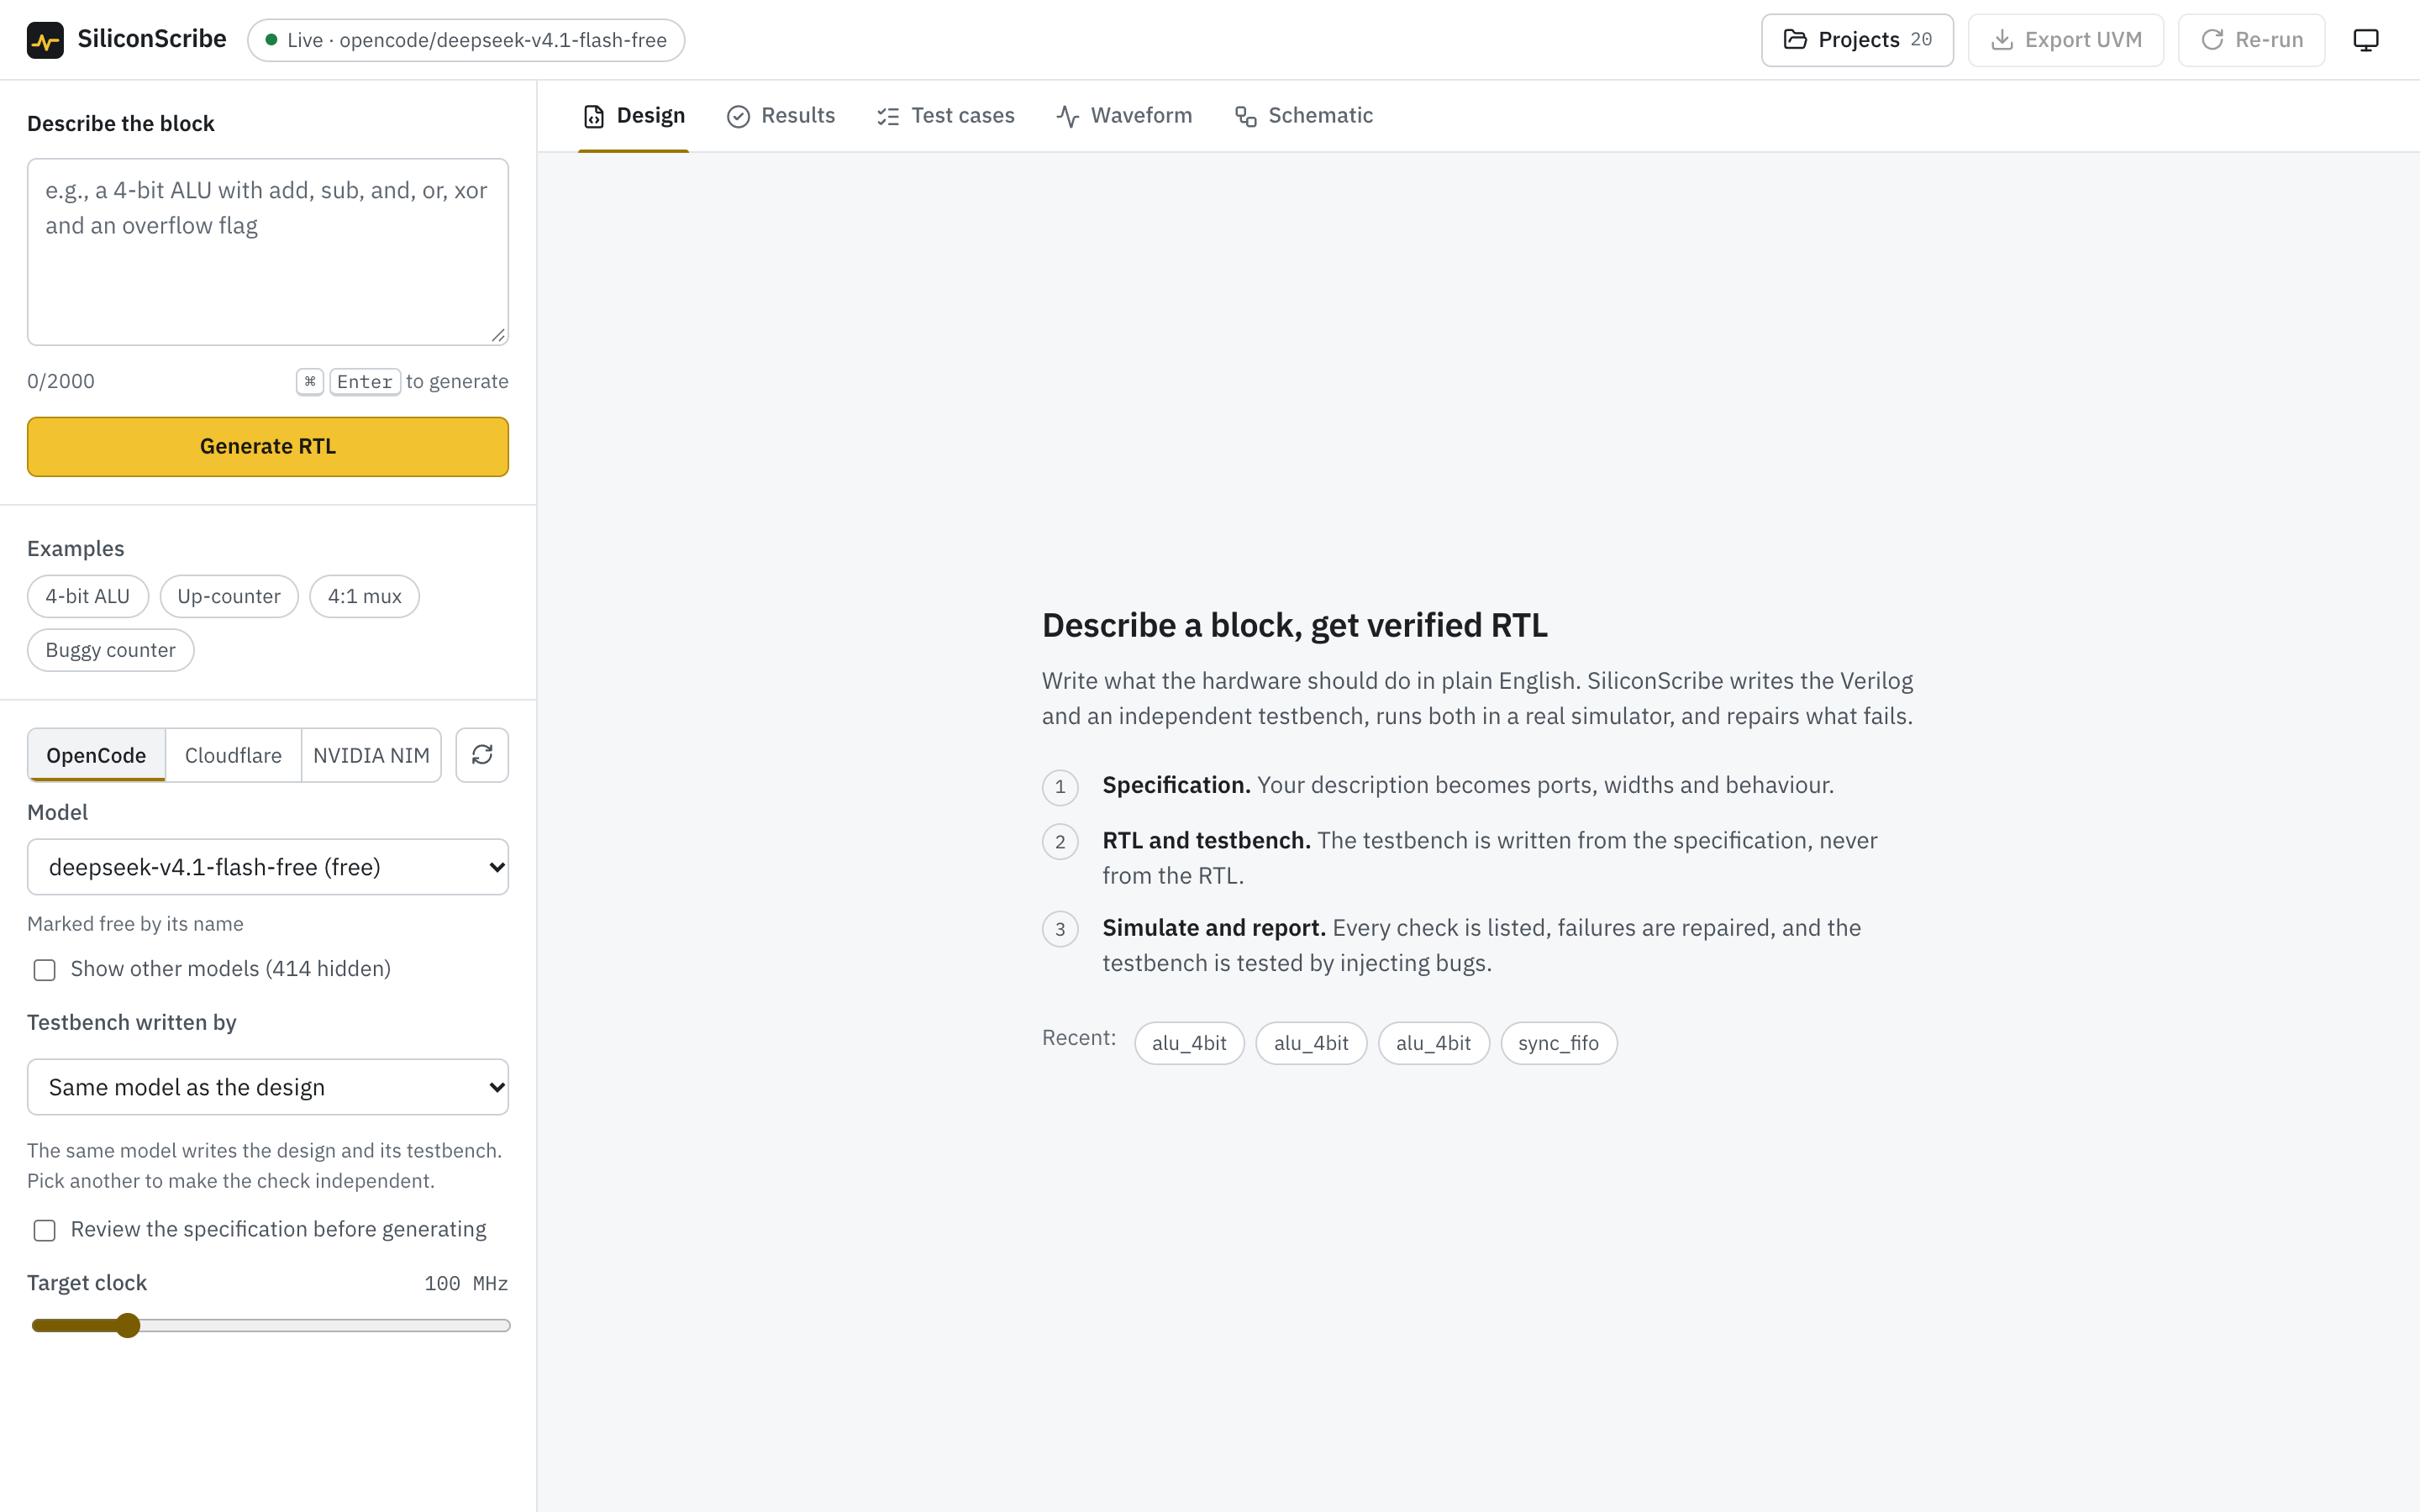
\includegraphics[width=0.92\textwidth]{s01_welcome.png}
\caption{Start screen of SiliconScribe. Before the first run, the Design tab explains the three steps and offers recent projects.}
\end{figure}

\section{The sidebar}

\begin{minipage}[t]{0.36\textwidth}
\vspace{0pt}
\centering
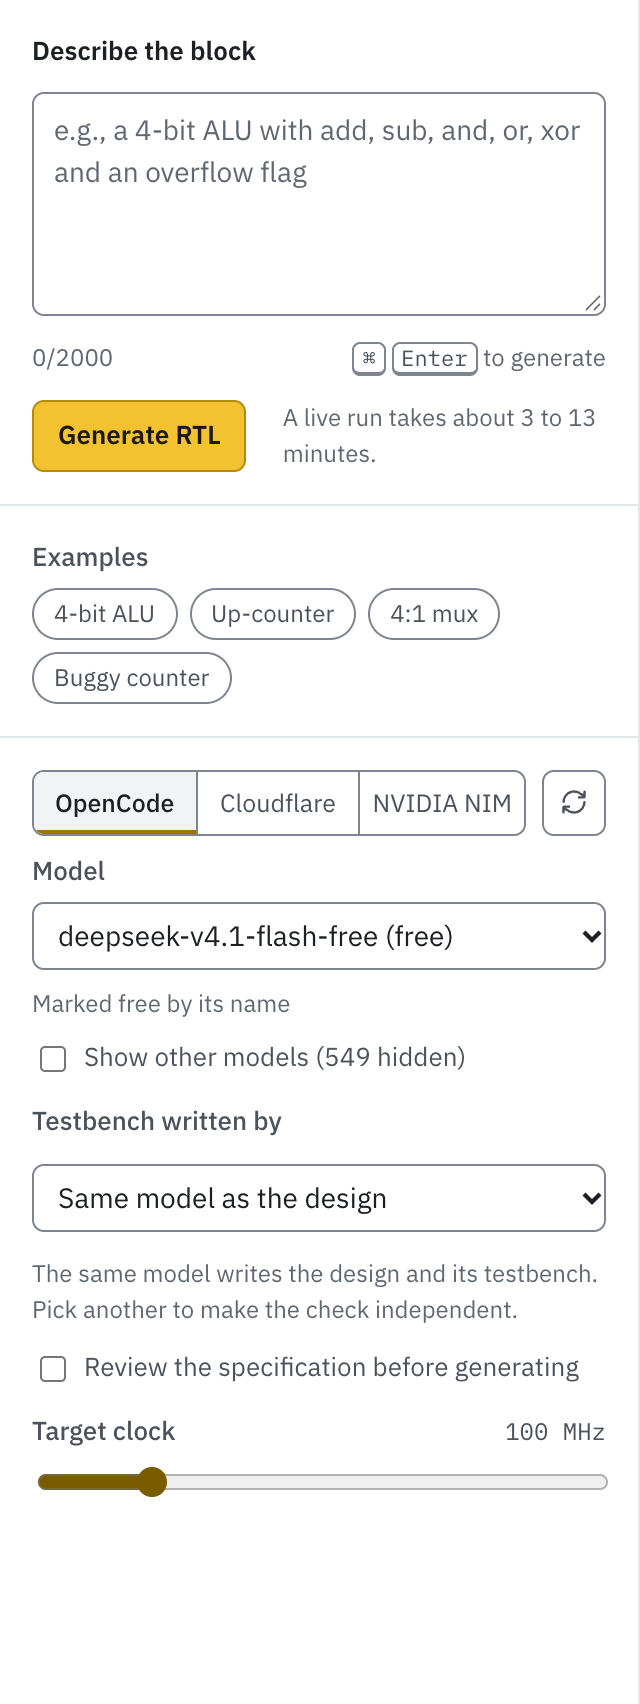
\includegraphics[height=0.52\textheight]{s02_model_menu.png}
\captionof{figure}{The sidebar with per-run model choice.}
\end{minipage}\hfill
\begin{minipage}[t]{0.6\textwidth}
\vspace{0pt}
From top to bottom:
\begin{description}
  \item[Describe the block] Up to 2000 characters, with a counter. Be specific about widths, reset style and behaviour. \textbf{Generate RTL} (or Ctrl/Cmd+Enter) starts the run.
  \item[Run] During and after a run, the run timeline appears right under the prompt (Section~\ref{sec:timeline}).
  \item[Examples] Four chips that fill the prompt: 4-bit ALU, Up-counter, 4:1 mux and Buggy counter (scripted only in offline mode).
  \item[Model menu] Three source tabs, \textbf{OpenCode}, \textbf{Cloudflare} and \textbf{NVIDIA NIM}, a refresh button, and the \textbf{Model} drop-down. Free models are marked ``(free)''; the note under the menu says why. On the OpenCode tab, \textbf{Show other models} lists the models not marked free (the number hidden is shown; they may use credits on your OpenCode account). Your choice is remembered in the browser.
  \item[Testbench written by] ``Same model as the design'' (default) or any other model from any tab. A separate model makes the check independent (Section~\ref{sec:independenttb}).
  \item[Review the specification before generating] When ticked, the run stops after the specification so you can check and edit it.
  \item[Target clock] 10 to 500 MHz (default 100). It is a hint for the RTL and the clock the timing estimate is checked against.
\end{description}
\end{minipage}

\section{Reviewing the specification}

With ``Review the specification before generating'' ticked, Generate RTL first asks the model only for the specification and shows it in the main pane: the module name, the ports (name, direction, width, description), any parameters, the \textbf{Behaviour} text and the \textbf{Constraints} (one per line). Correct anything that does not match what you meant, then press \textbf{Generate with this specification}; the run uses exactly that specification. \textbf{Cancel} goes back. This is not available in offline mode.

\begin{figure}[H]
\centering
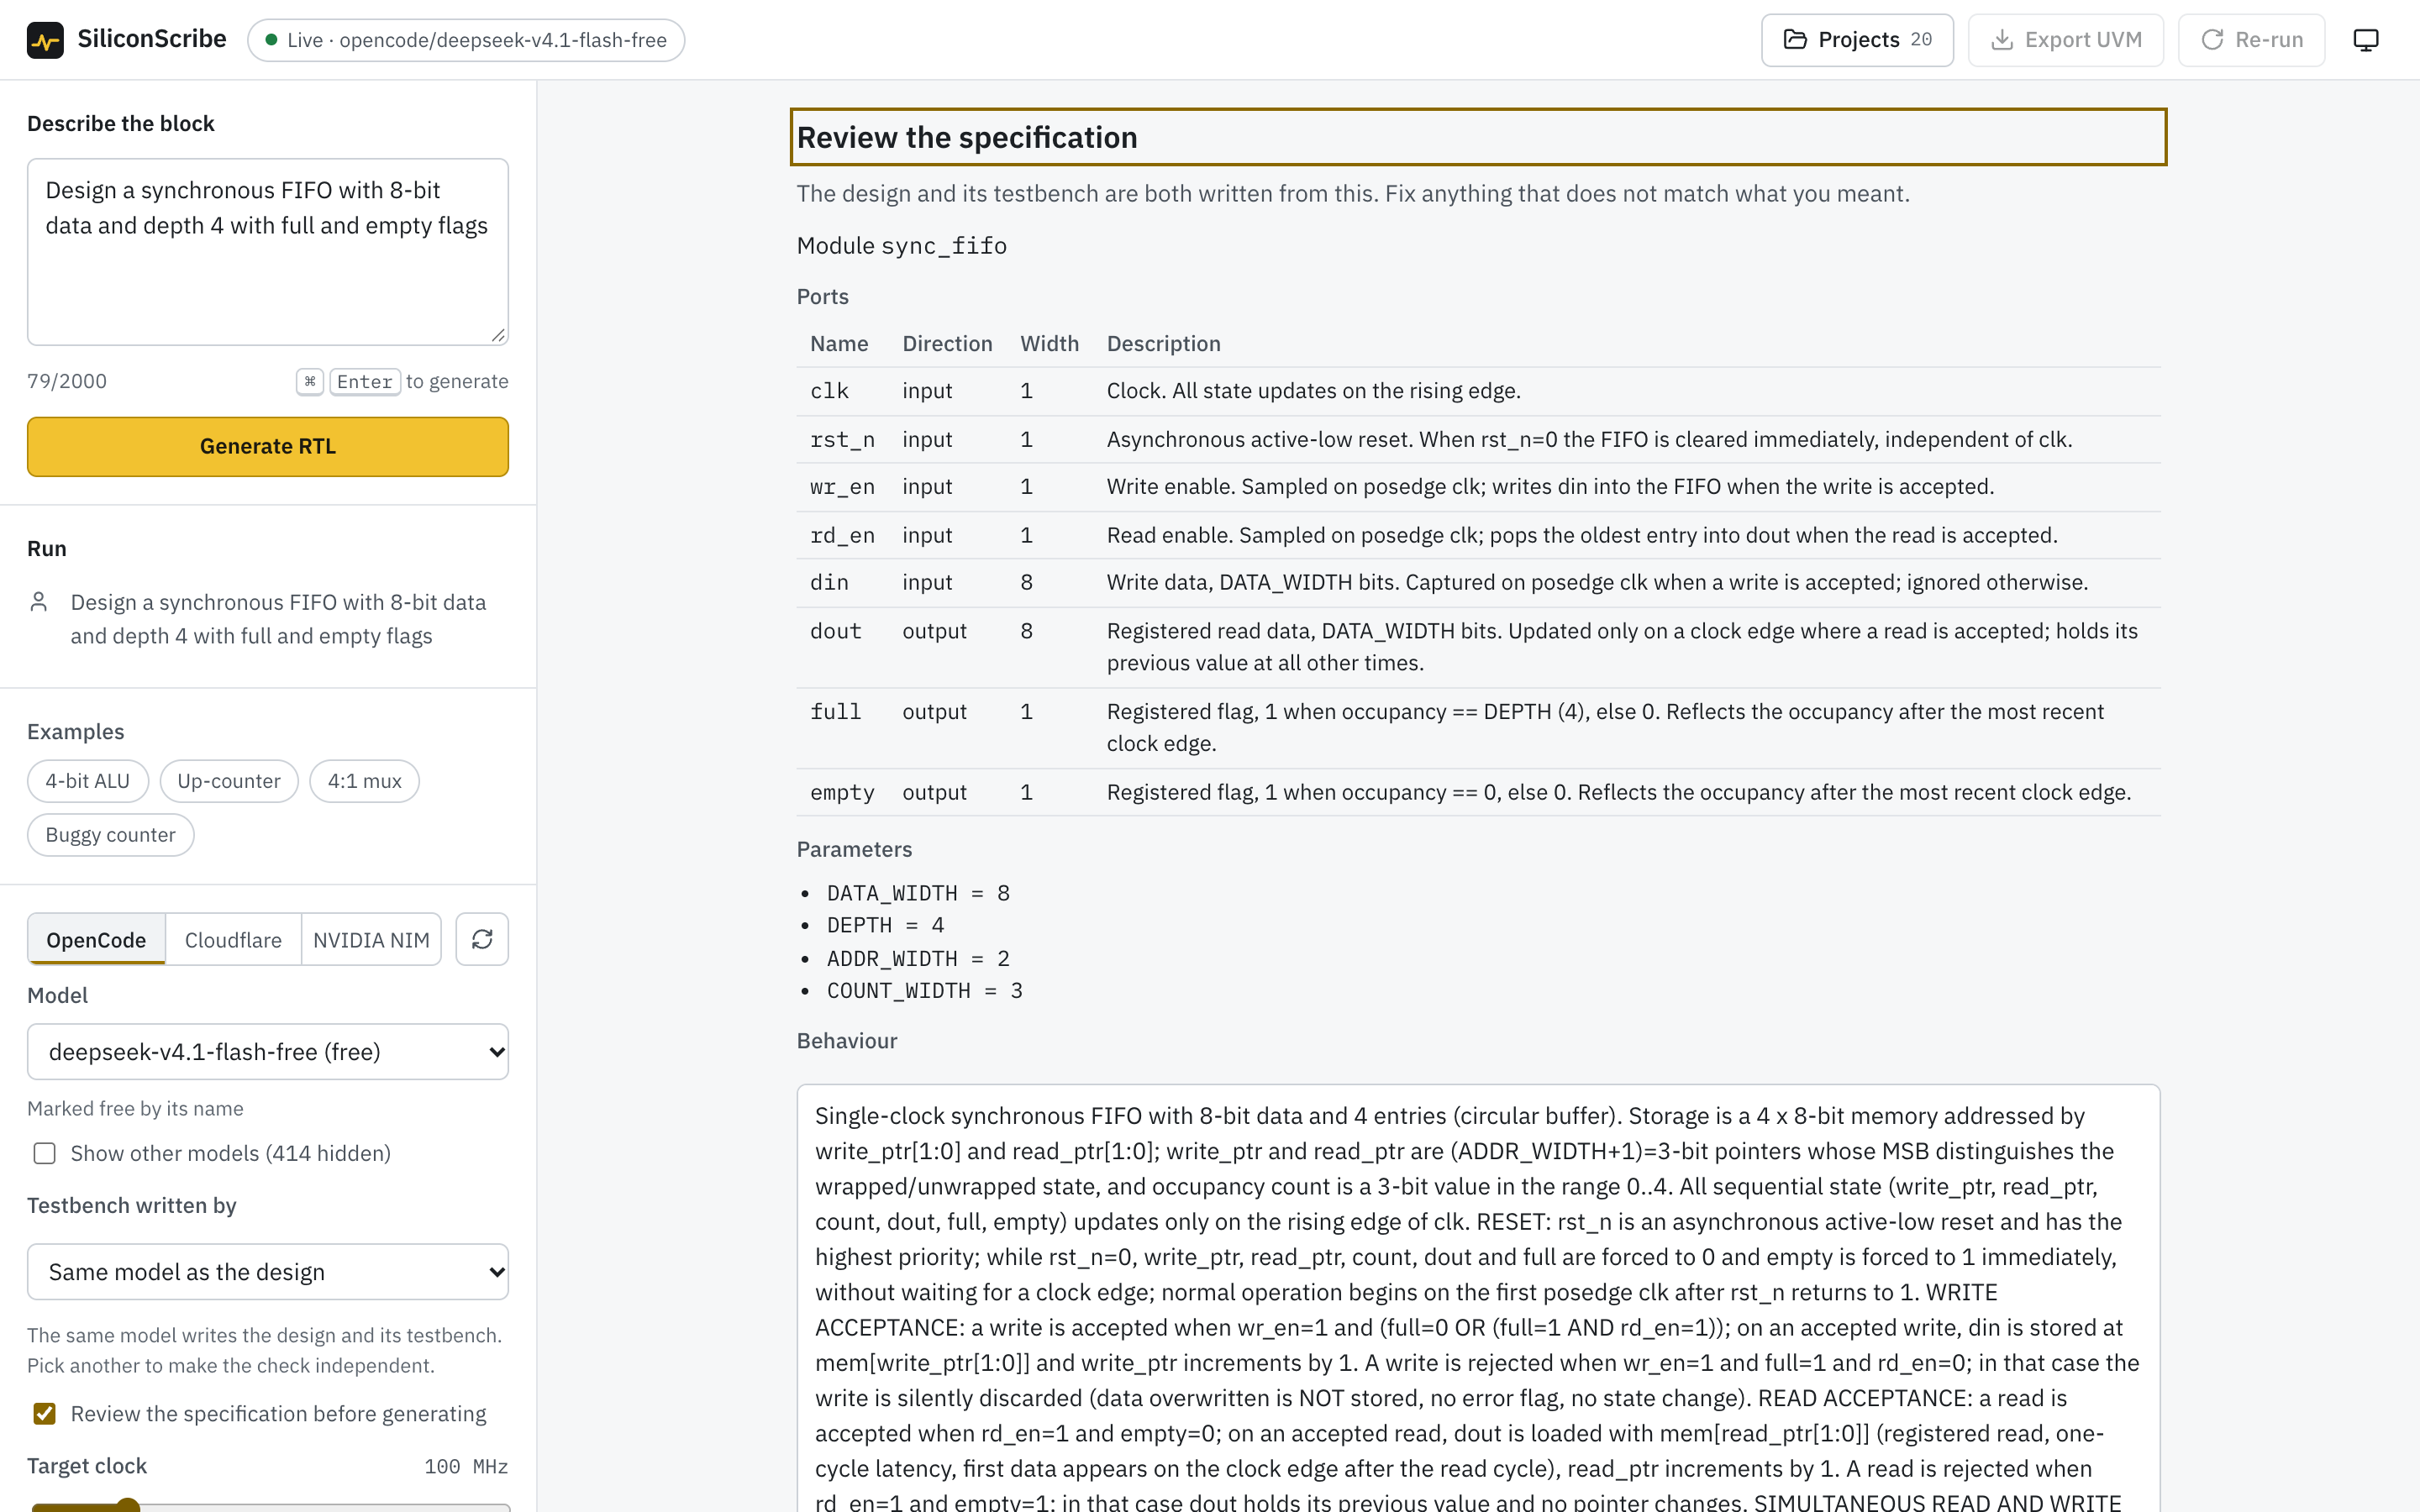
\includegraphics[width=0.92\textwidth]{s04_spec_review.png}
\caption{Reviewing the parsed specification before generation (a real specification written by the live model for a FIFO prompt).}
\end{figure}

\section{Watching the run}
\label{sec:timeline}

The run timeline lists one line per step: specification, RTL, lint, testbench, explanation, each simulation, each repair with its diagnosis (symptom, root cause, fix location, confidence), synthesis, the second opinion when there is one, testbench strength, timing, and the final message. While the run is going, a ``Working\ldots'' timer shows it is not stuck. Free models can take minutes per step. \textbf{Stop} in the top bar cancels the run.

\begin{figure}[H]
\centering
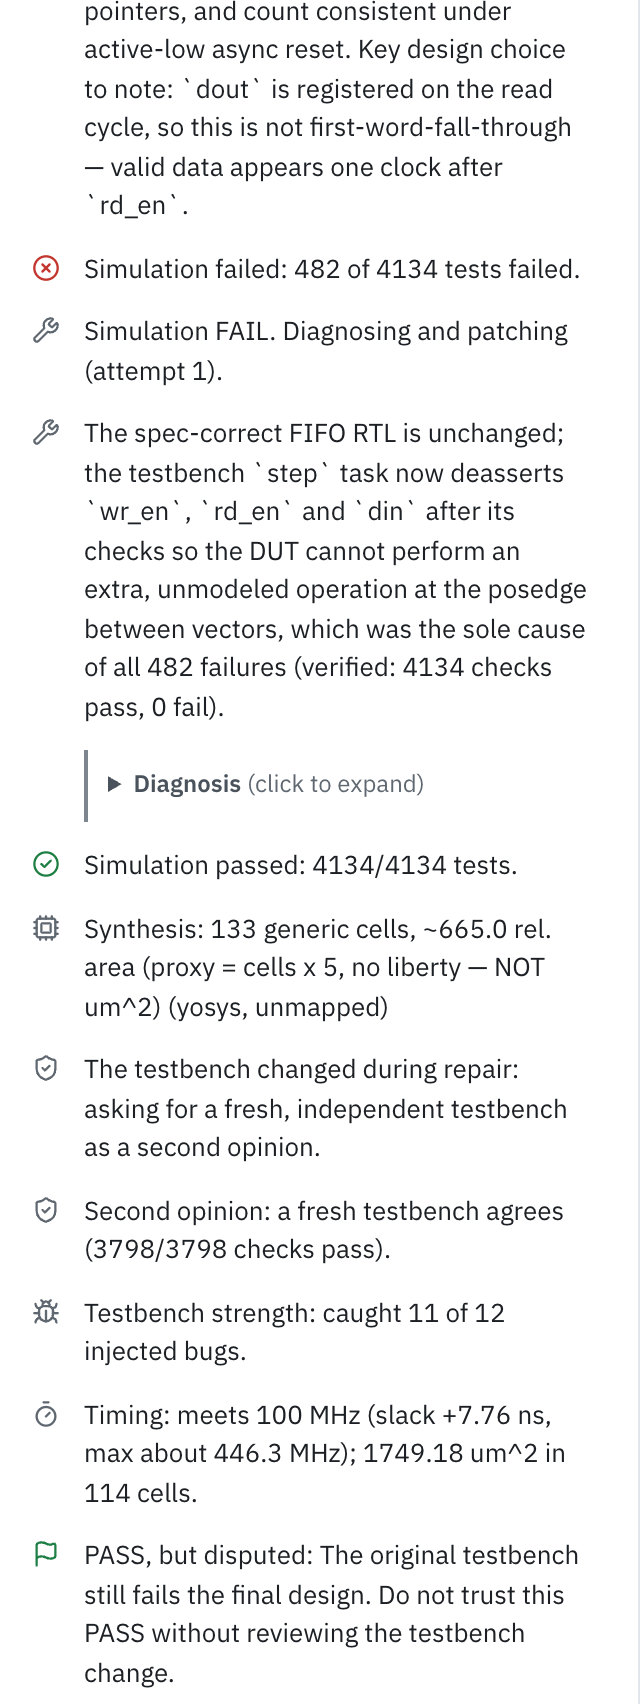
\includegraphics[height=0.5\textheight]{s05_run_timeline.png}
\caption{The run timeline of a real FIFO run (opencode/hy4-flash-free): one repair, then the second opinion, strength and timing steps.}
\end{figure}

\section{A first run, step by step}

\begin{enumerate}
  \item Click an example or type your own description.
  \item Choose a model (or keep the default), and optionally a separate testbench model, the specification review and a target clock.
  \item Press \textbf{Generate RTL}. The Design tab shows the code as it arrives; the timeline shows each step.
  \item When the run ends, the Results tab opens. Read the verdict first, then the sections below it.
  \item Open \textbf{Test cases} to see every check, \textbf{Waveform} to see the signals, \textbf{Schematic} for the block diagram.
  \item The run is saved automatically and appears in the \textbf{Projects} menu.
\end{enumerate}

\section{Reading the Results tab}

\begin{figure}[H]
\centering
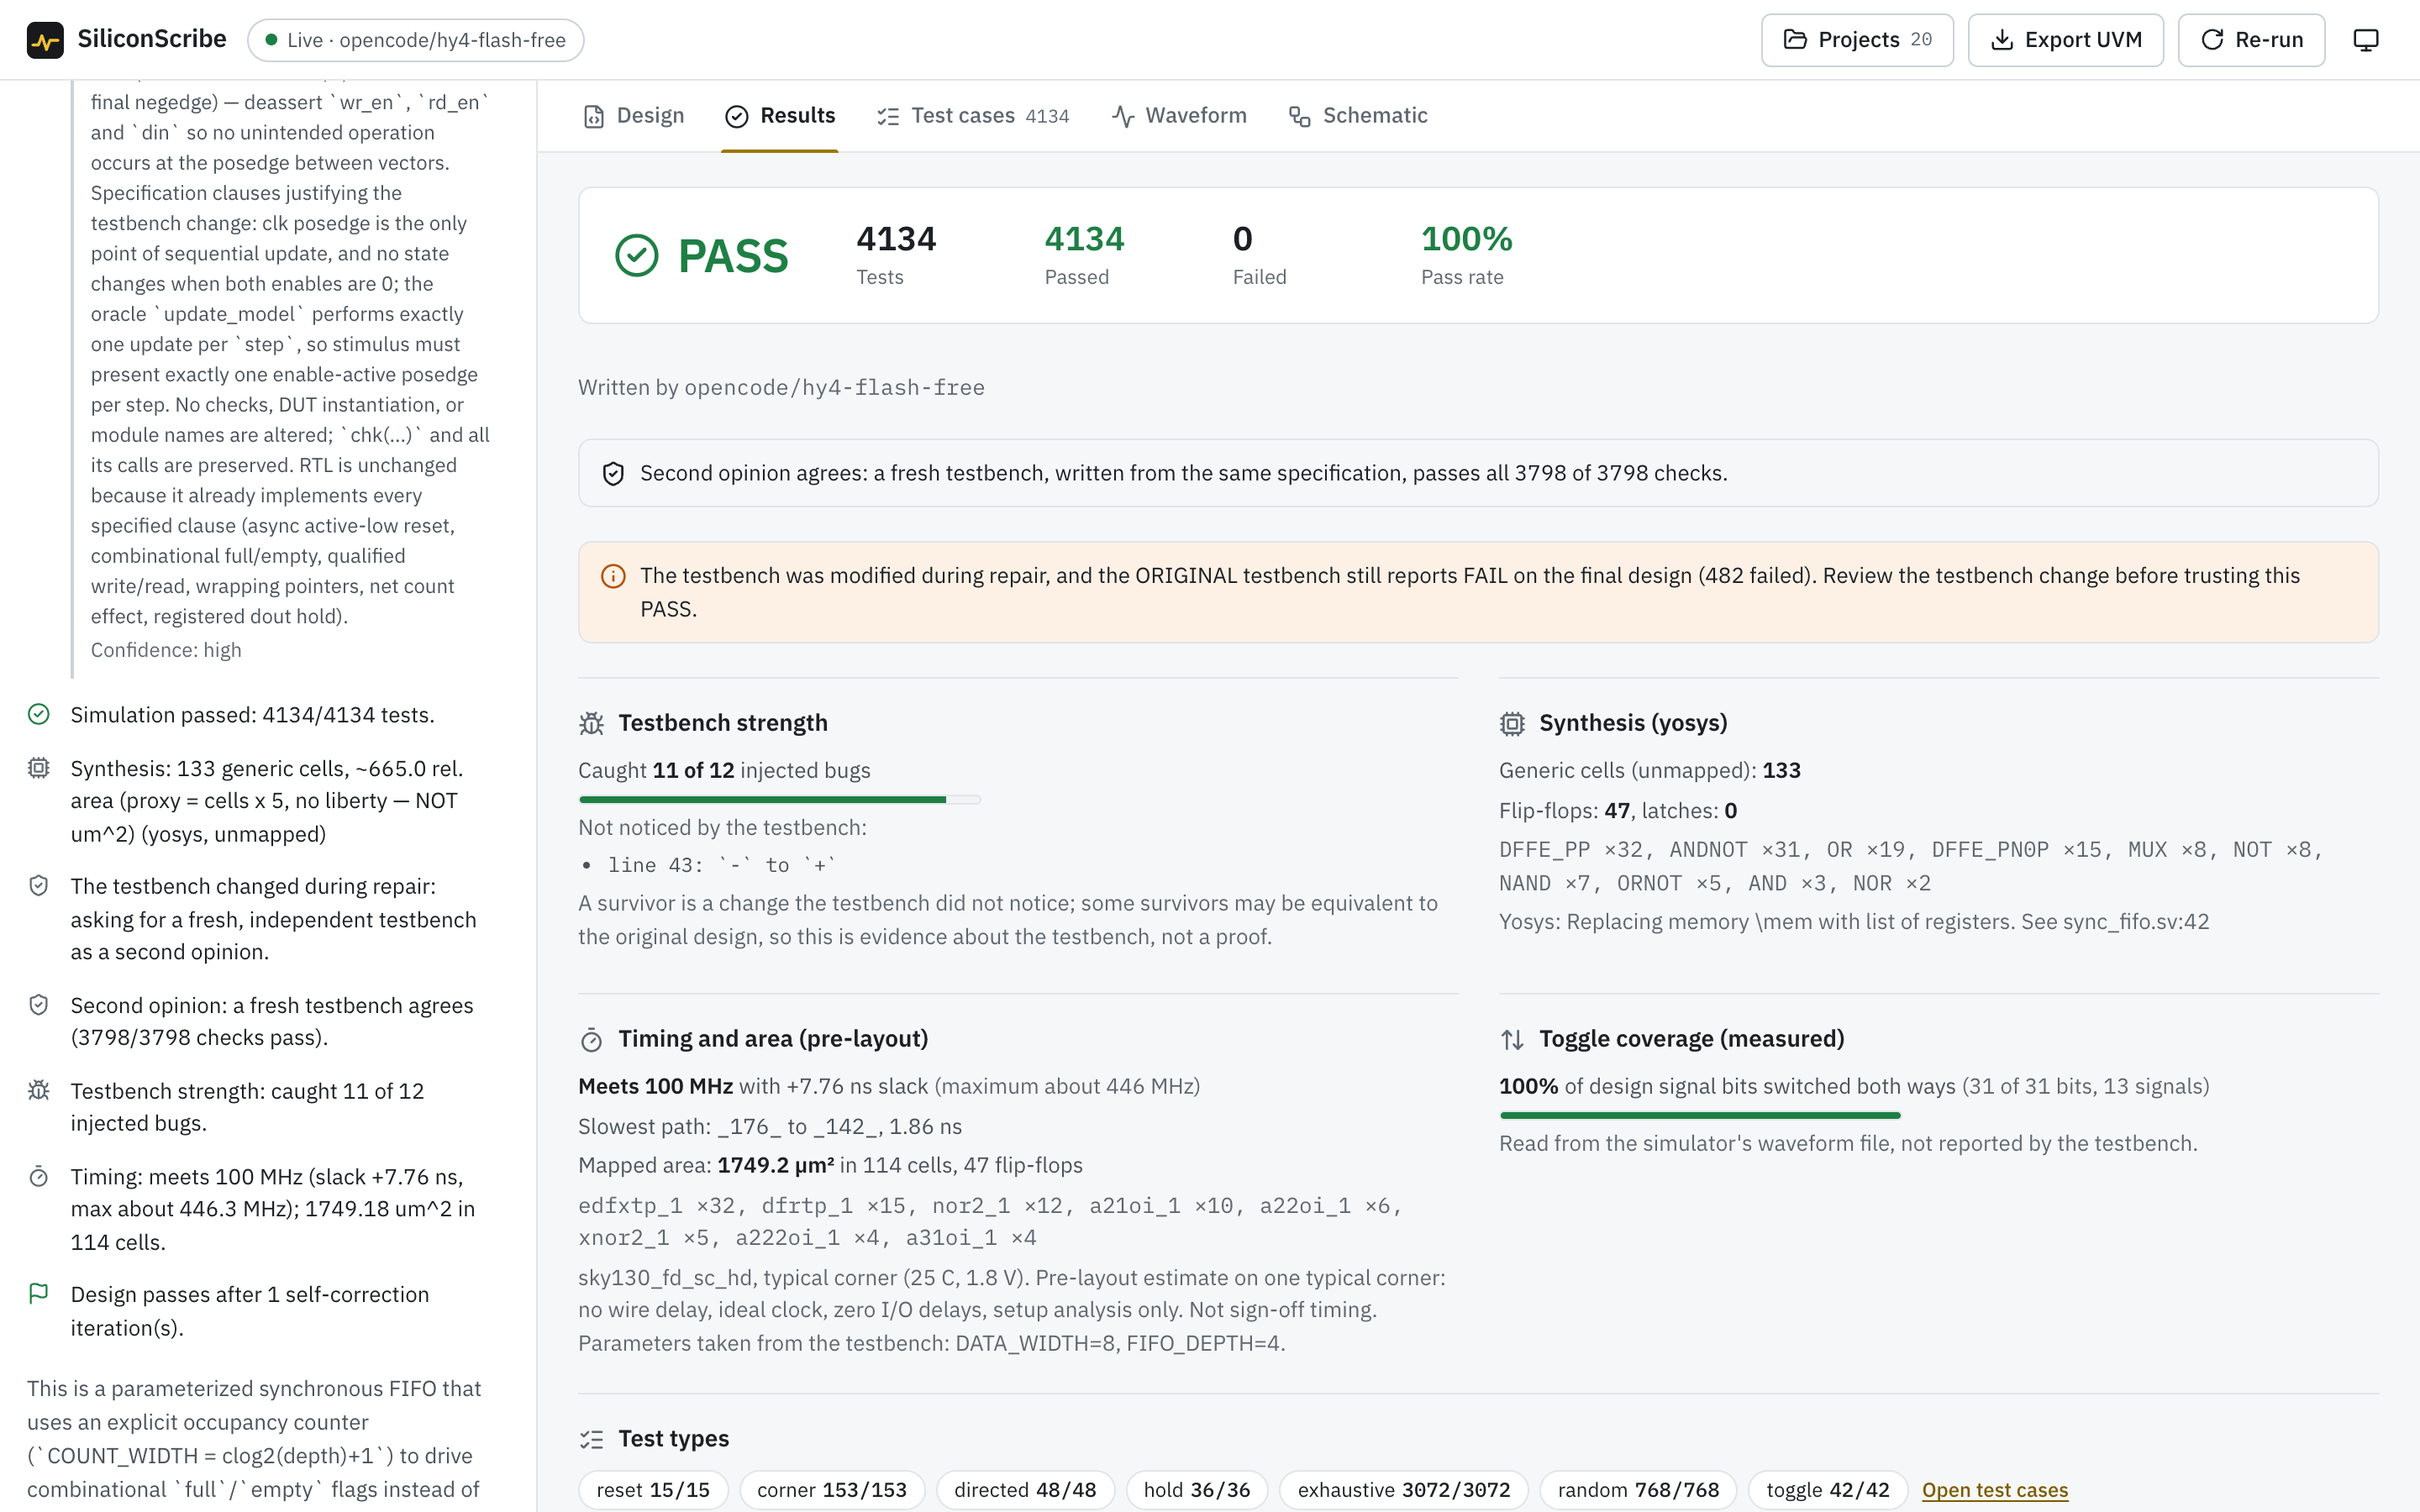
\includegraphics[width=0.95\textwidth]{s06_results_pass.png}
\caption{Results of a real FIFO run (opencode/hy4-flash-free): PASS 4134/4134 after one repair, the second opinion agrees (3798/3798), and a warning that the original testbench still fails on the final design (482 failed). Strength 11 of 12, timing meets 100 MHz, toggle coverage 100\%.}
\end{figure}

\begin{description}
  \item[Verdict] The status badge and four numbers: Tests, Passed, Failed, Pass rate. PASS (the design ran and every check passed), FAIL (some checks failed), ERROR (compile or runtime problem, no valid summary, or zero checks), TIMEOUT (the simulation ran too long). These come from the simulator transcript, never from the model.
  \item[Written by] The model that wrote the design, and, if a separate model wrote the testbench, ``Testbench written by \ldots, a separate model''. It is not shown for an offline result or after a Re-run of edited code.
  \item[Second opinion] Shown only when a repair rewrote the testbench: agrees, disagrees (do not trust this PASS) or not obtained, with the reason.
  \item[Warnings] Amber notes such as too few checks, a weak testbench, the original testbench still failing, or two models disagreeing. A grey ``Built-in demo result: not generated by the AI model for your prompt'' note marks a demo fallback.
  \item[Testbench strength] ``Caught N of M injected bugs'' with a bar, and the bugs that were not noticed (line and change). The bar turns amber when fewer than half were caught. A survivor may be an equivalent change (Section~\ref{sec:strength}).
  \item[Synthesis (yosys)] Generic (unmapped) cell count, flip-flops and latches, cell types, and any Yosys warning (with file names only, never the server's folder paths). The relative area proxy appears only when there is no mapped area.
  \item[Timing and area (pre-layout)] ``Meets'' or ``Misses'' the target clock with the slack and the maximum frequency; for a design with no clock, ``Longest input-to-output path'' instead. Then the slowest path, the mapped area in \umsq{} with cell and flip-flop counts, the most common cells, and the limits line (one corner, no wire delay, ideal clock, setup only, not sign-off). If the estimate refused the design, the reason is shown instead of a number.
  \item[Toggle coverage (measured)] The percentage of design signal bits that switched both ways, with counts and the signals that never switched. It is read from the simulator's waveform file.
  \item[Test types] One chip per type of check (for example reset, corner, directed, hold, random), with ``Open test cases''.
  \item[Lint, Self-correction loop, Errors] Lint findings; each repair attempt with its status, counts and fix type (\emph{compiler\_repair} and \emph{llm\_diagnosis} are real fixes; \emph{offline\_scripted} is the labelled demo path with no invented root cause); the error lines of a failed run.
  \item[Specification the design was built from] A fold-out, read-only copy of the specification that was used.
\end{description}

\begin{figure}[H]
\centering
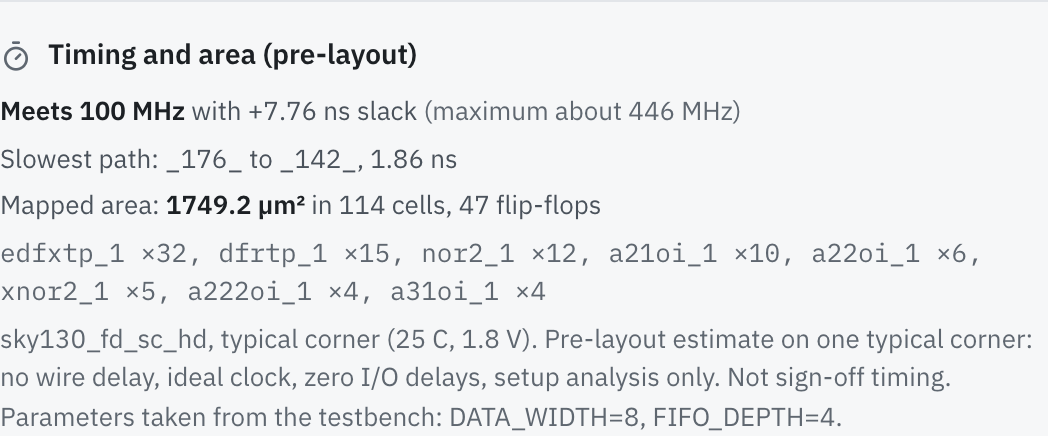
\includegraphics[width=0.62\textwidth]{s07_timing_section.png}
\caption{The ``Timing and area (pre-layout)'' section with its limits line.}
\end{figure}

\begin{figure}[H]
\centering
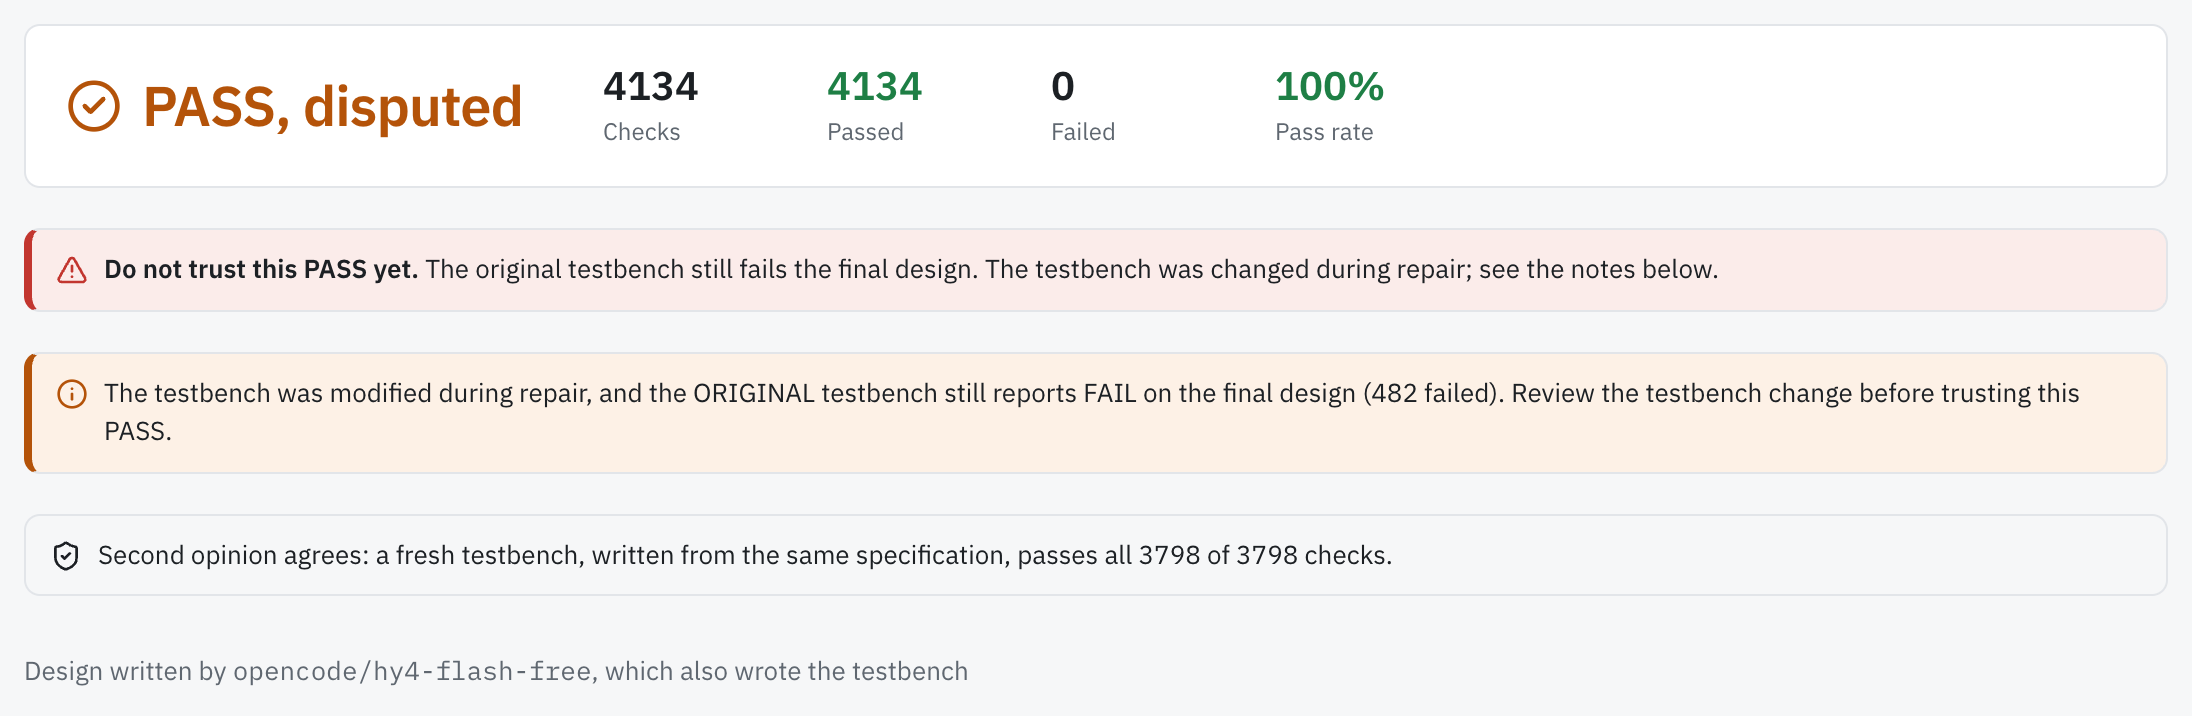
\includegraphics[width=0.92\textwidth]{s08_second_opinion.png}
\caption{The second opinion and the testbench-change warning are both shown.}
\end{figure}

\section{The Test cases tab}
\label{sec:testcases}

The Results tab only says ``4134 passed''. The Test cases tab shows \emph{which} checks ran. At the top, a bar and the totals; below it one chip per test type showing how many of that type passed; click a chip to filter. The table lists each check's number, type, name, simulation time, expected value, actual value and result. Use the Failed filter to see only failures, search by name, or click a row to see a bit-by-bit comparison with the differing bits highlighted and a \textbf{Show in waveform} button that jumps to that moment. Long runs stay fast because only the visible rows are drawn, and a note says when the list is capped (the totals are always exact). Testbenches that do not use the standard \texttt{chk} task show only totals, and the tab says so rather than inventing a list.

\begin{figure}[H]
\centering
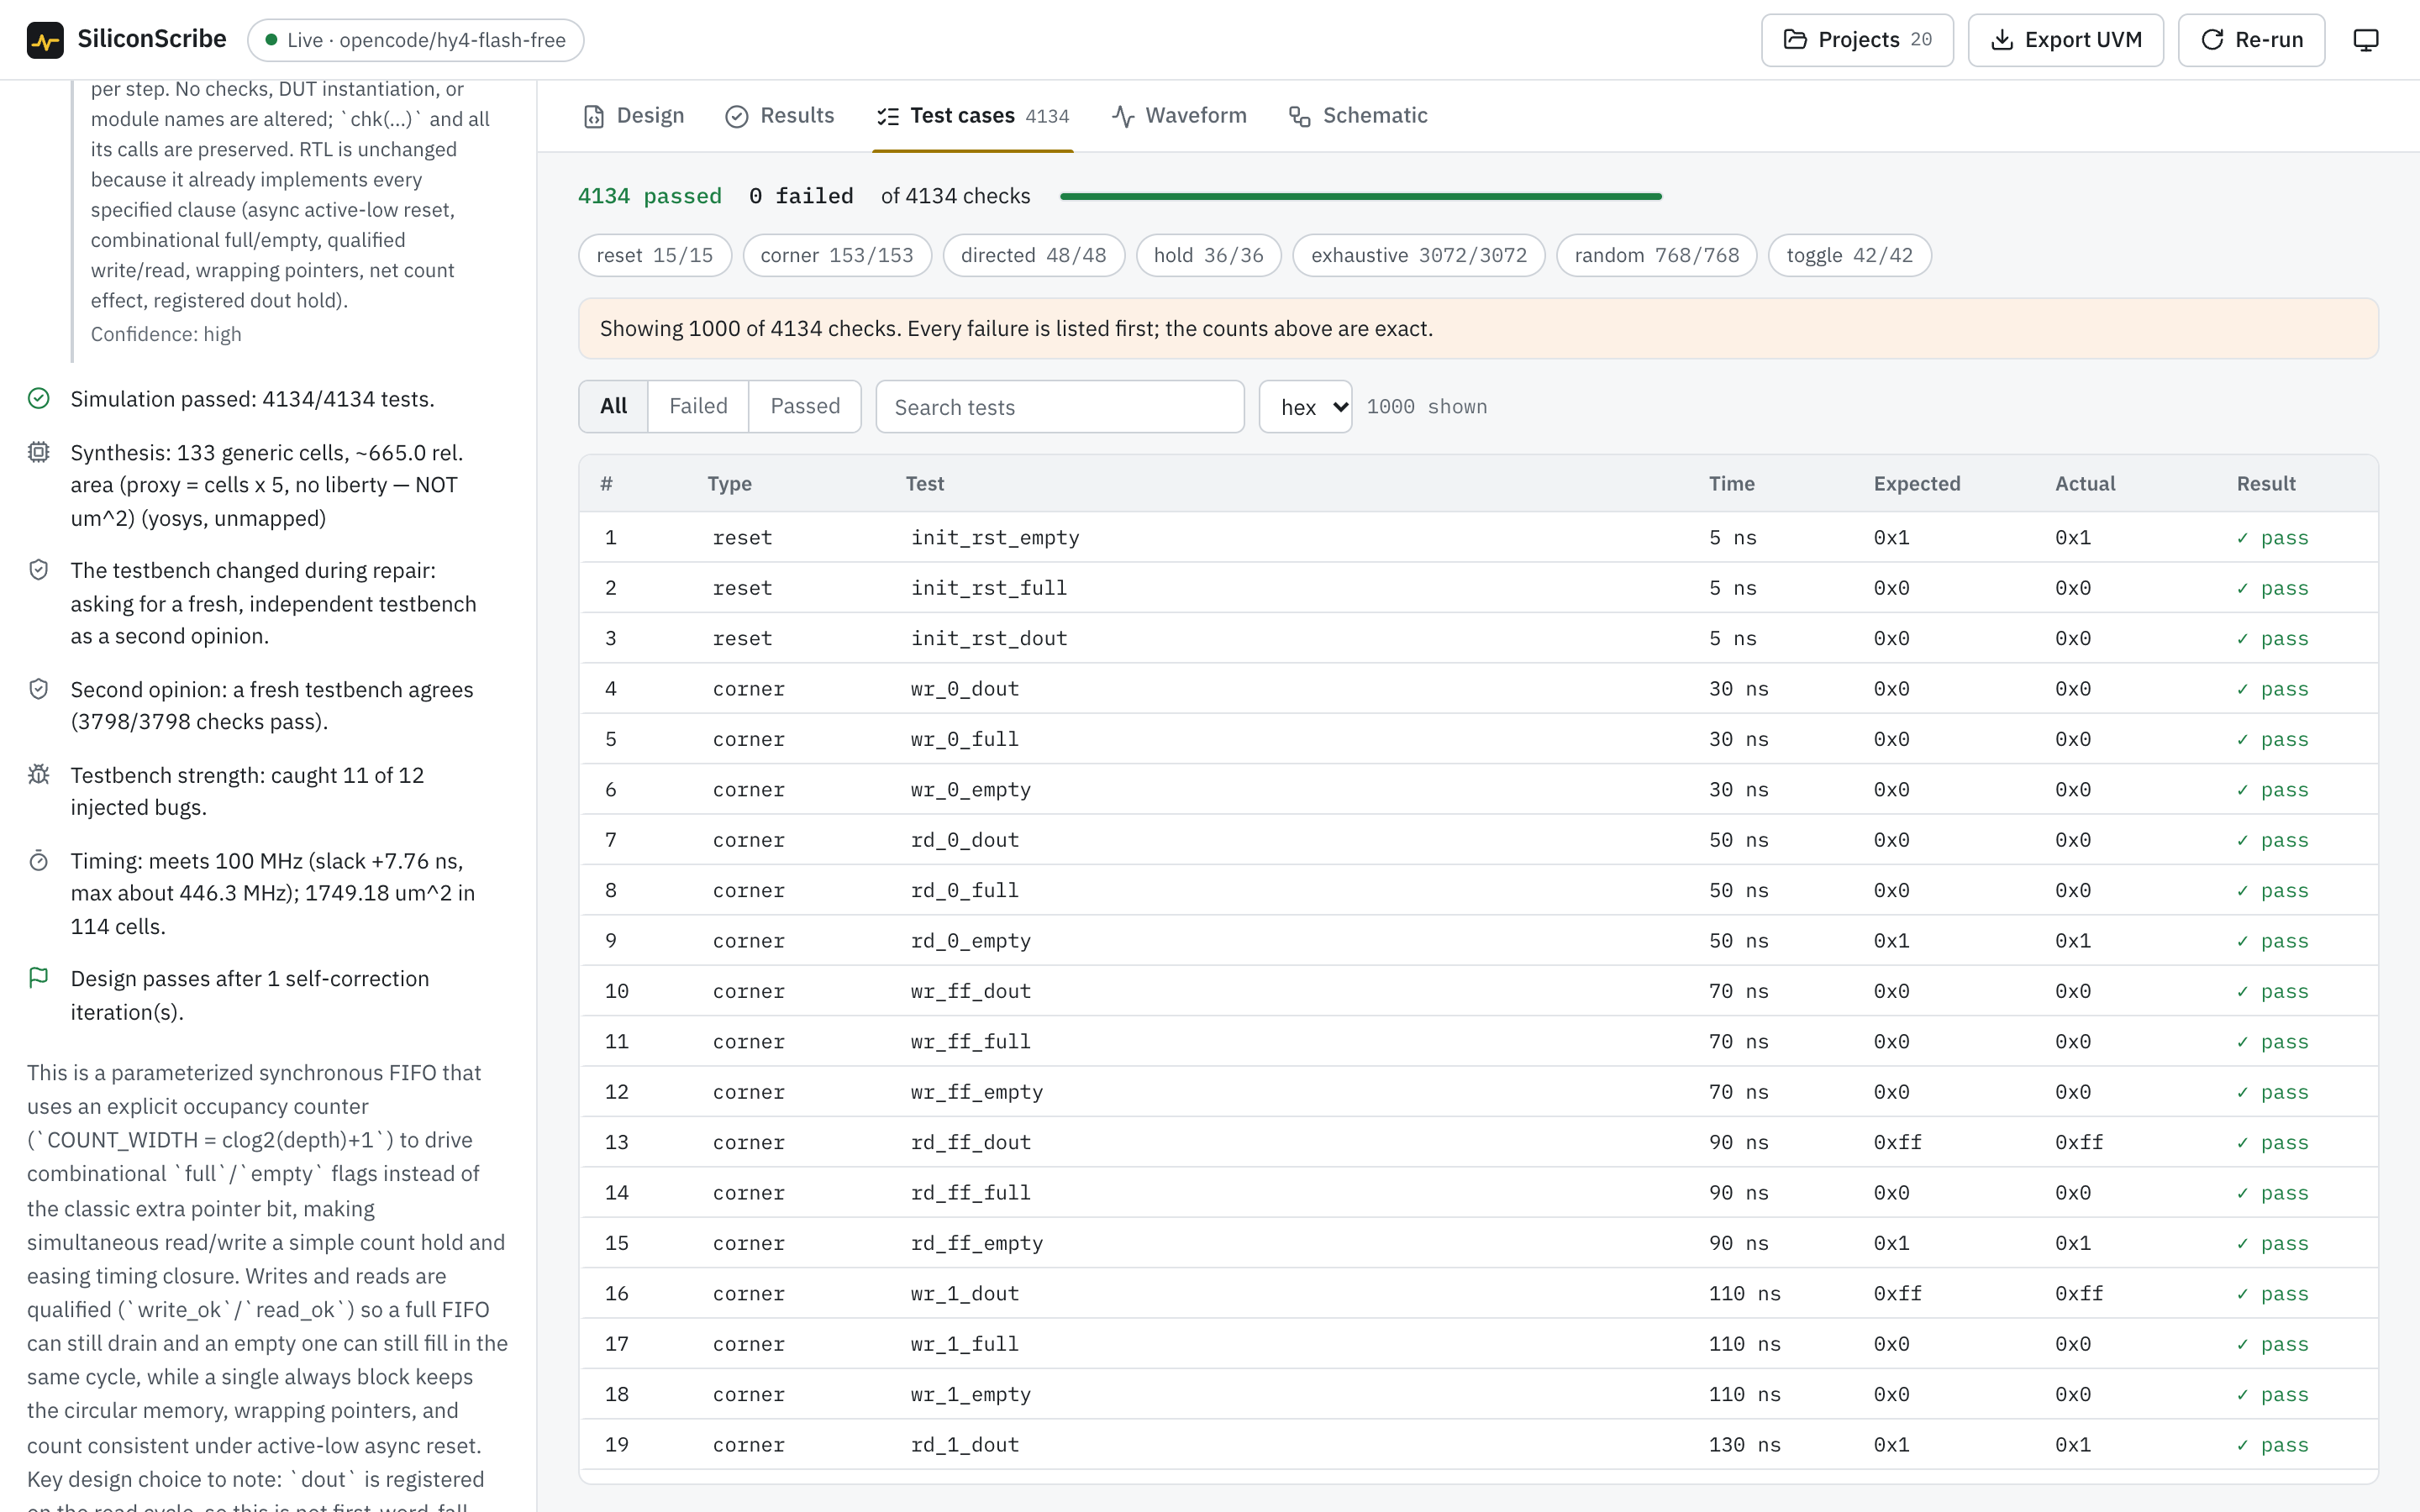
\includegraphics[width=0.92\textwidth]{s09_test_cases.png}
\caption{The Test cases tab of the FIFO run: 4134 checks grouped by type.}
\end{figure}

\section{The Waveform tab}

The waveform opens fitted to the pane. Signals are grouped by role (clock and reset, inputs, outputs, internal); the testbench's own variables are hidden until you ask for them. Click the plot to place cursor A, Shift+click for cursor B (the readout shows the time difference), and the signal-name column shows every signal's value at the cursor in hex, binary or decimal. Red flags on the time axis mark failed checks; press \texttt{]} and \texttt{[} to step between them. Use + and $-$ (or Ctrl/Cmd and the scroll wheel) to zoom and Reset to fit again, and \textbf{Expand} to give the whole results pane the full window (Esc restores it).

\begin{figure}[H]
\centering
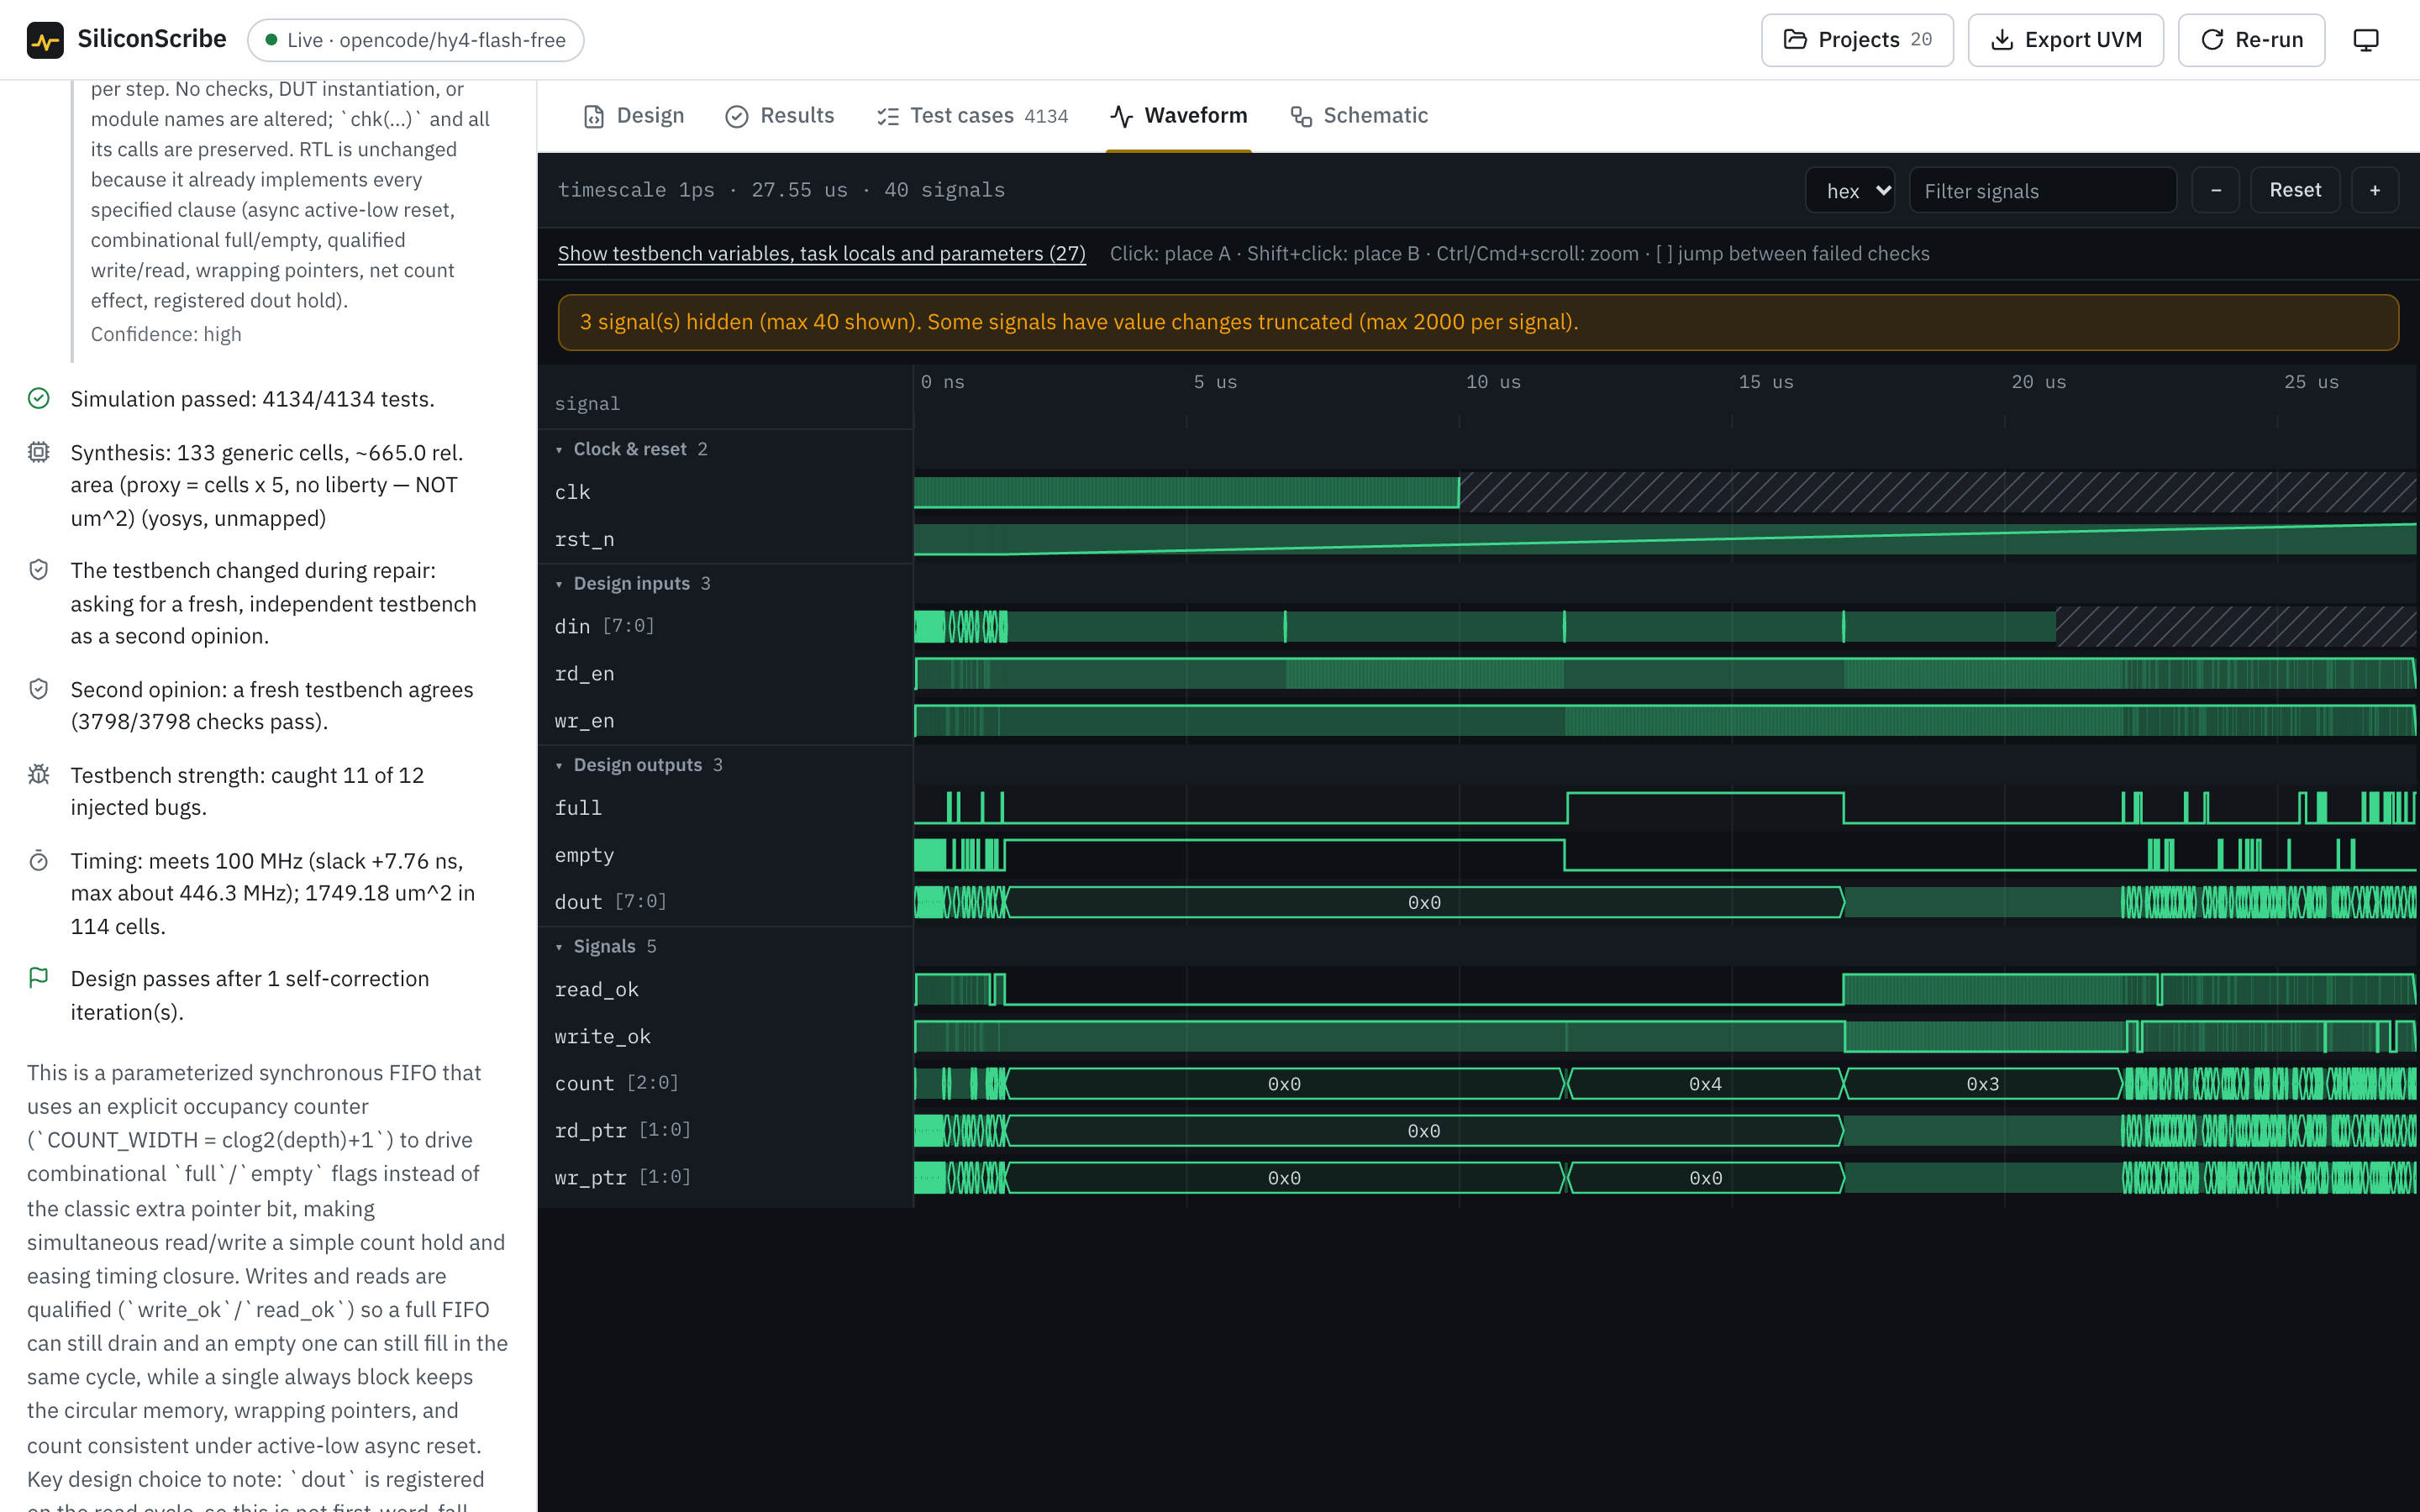
\includegraphics[width=0.92\textwidth]{s10_waveform.png}
\caption{The Waveform tab of the FIFO run.}
\end{figure}

\section{The Schematic and Design tabs}

The Schematic tab shows a port-level block diagram: the module as a box with inputs on the left, outputs on the right and widths such as \code{[7:0]}. A gate-level view of the synthesized netlist is not drawn; the tab says it is future work. The Design tab holds the RTL and testbench editors.

\begin{figure}[H]
\centering
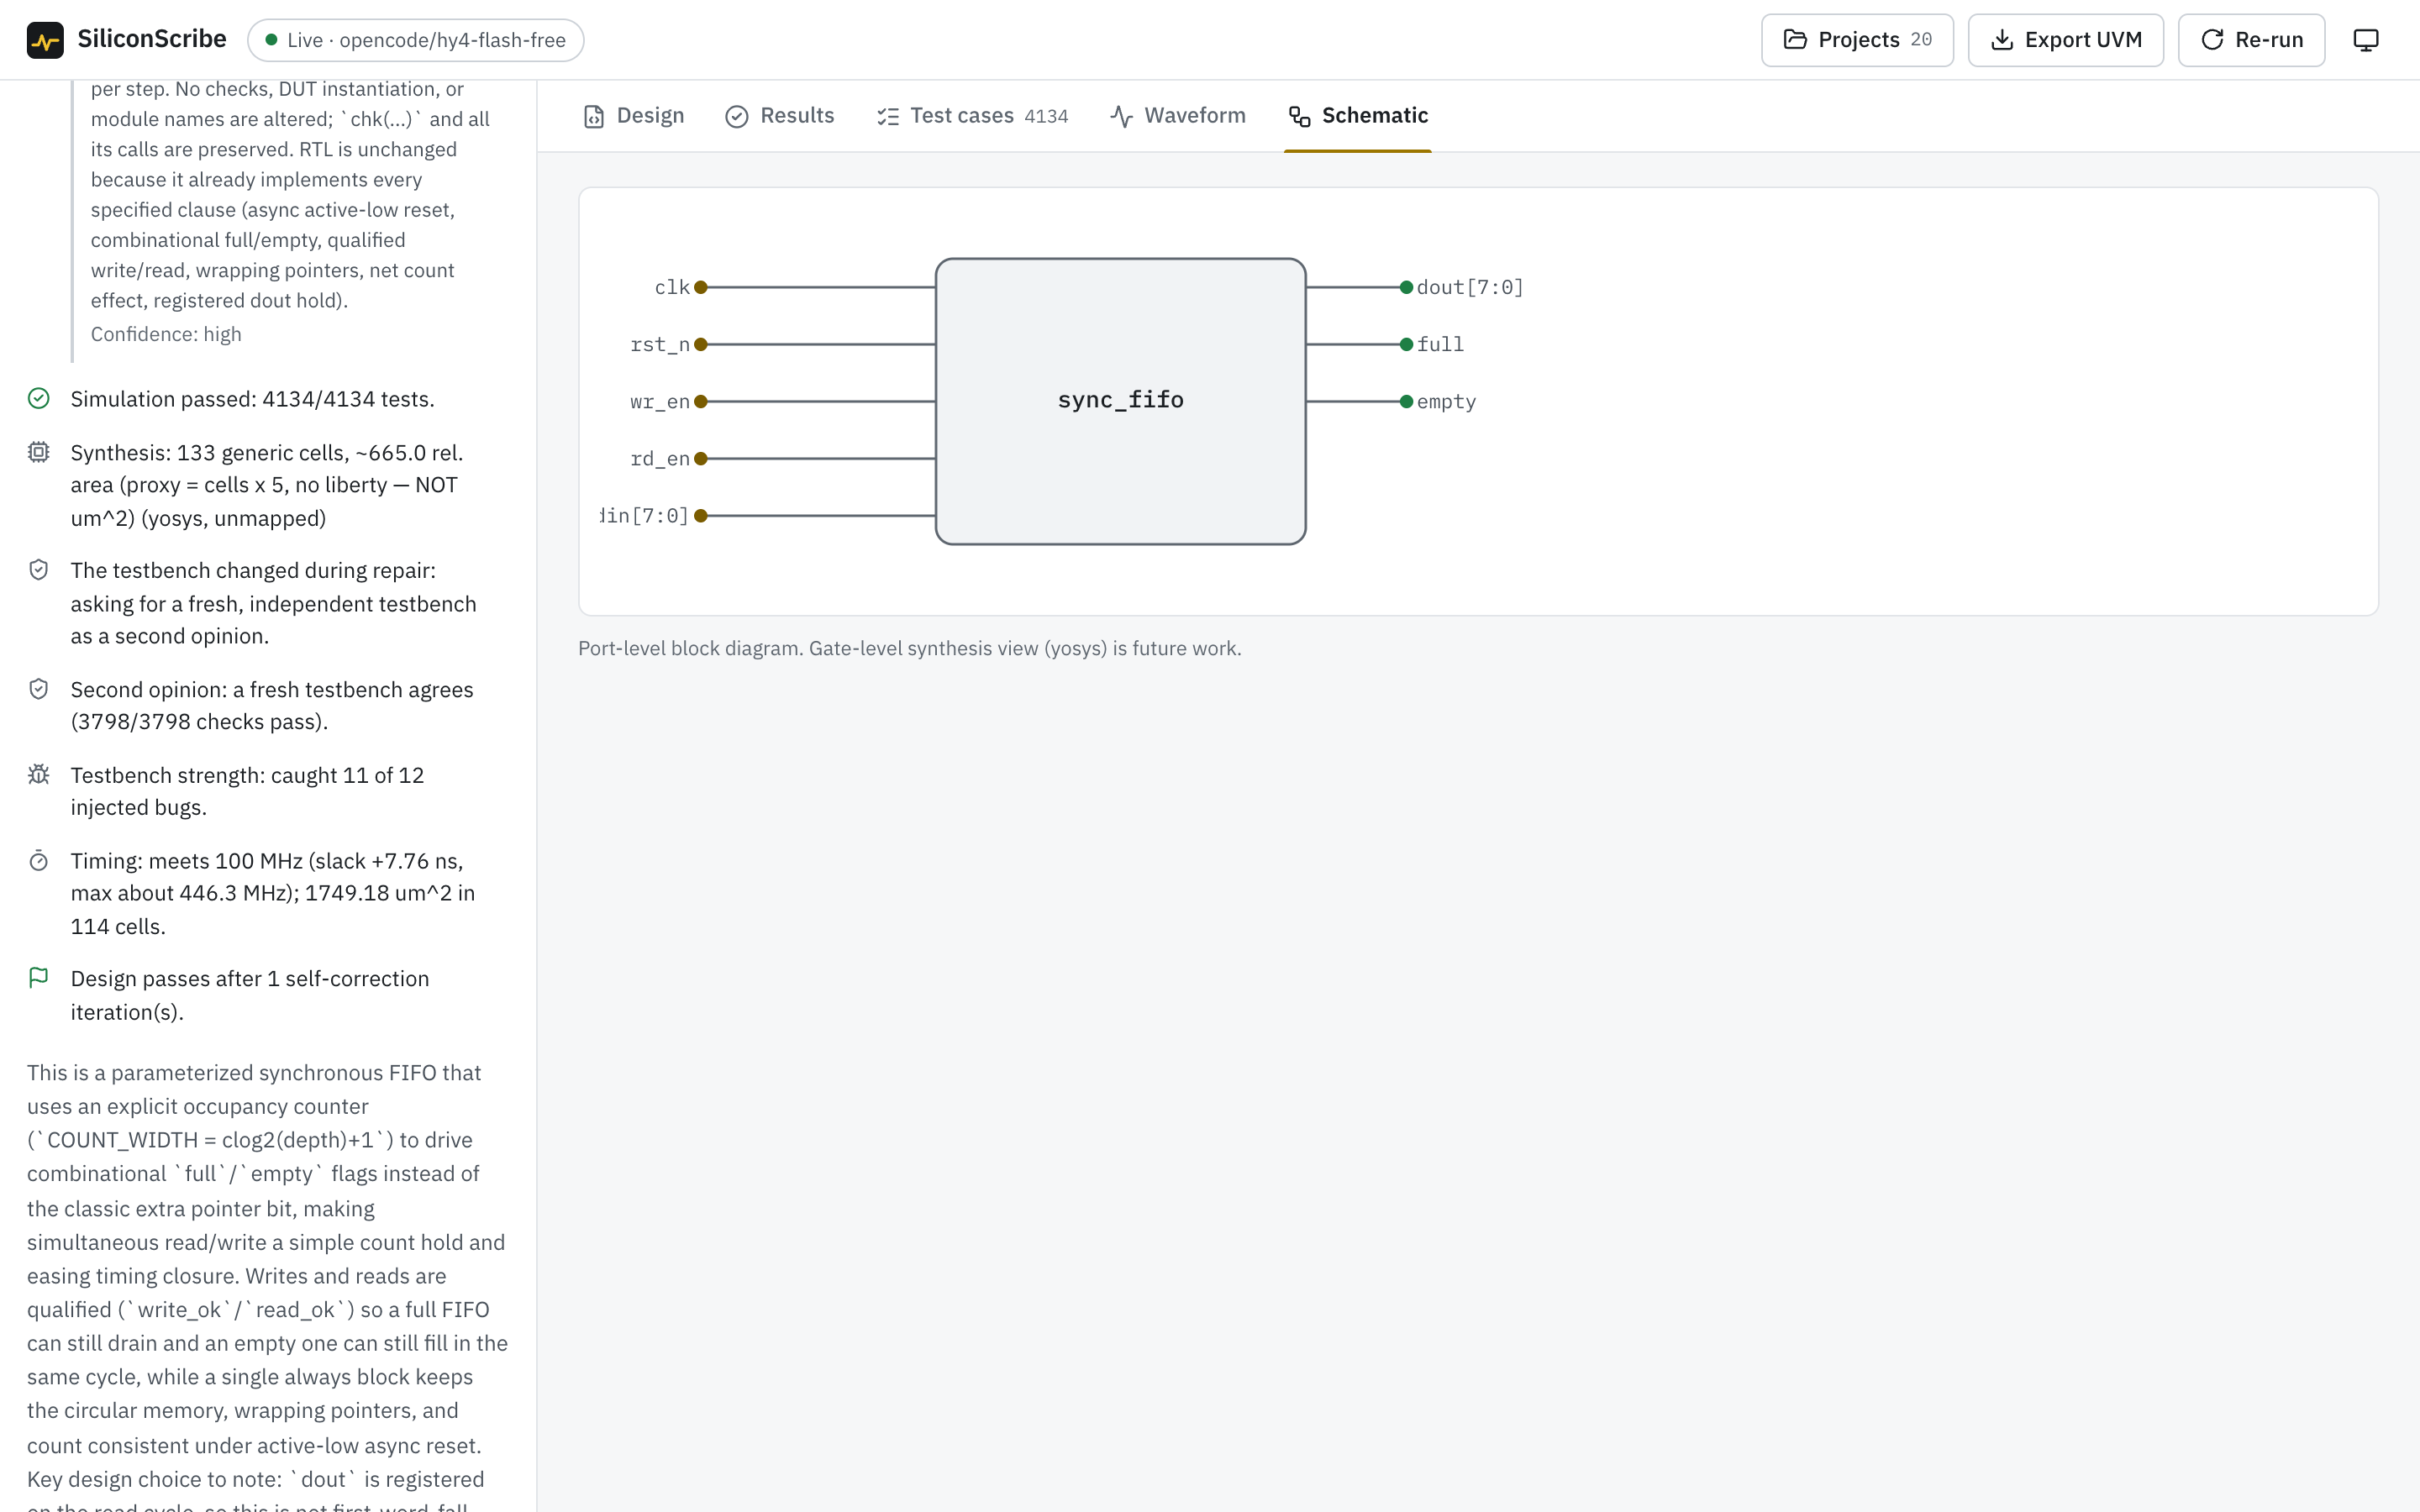
\includegraphics[width=0.92\textwidth]{s11_schematic.png}
\caption{The Schematic tab: a port-level block diagram of the FIFO.}
\end{figure}

\begin{figure}[H]
\centering
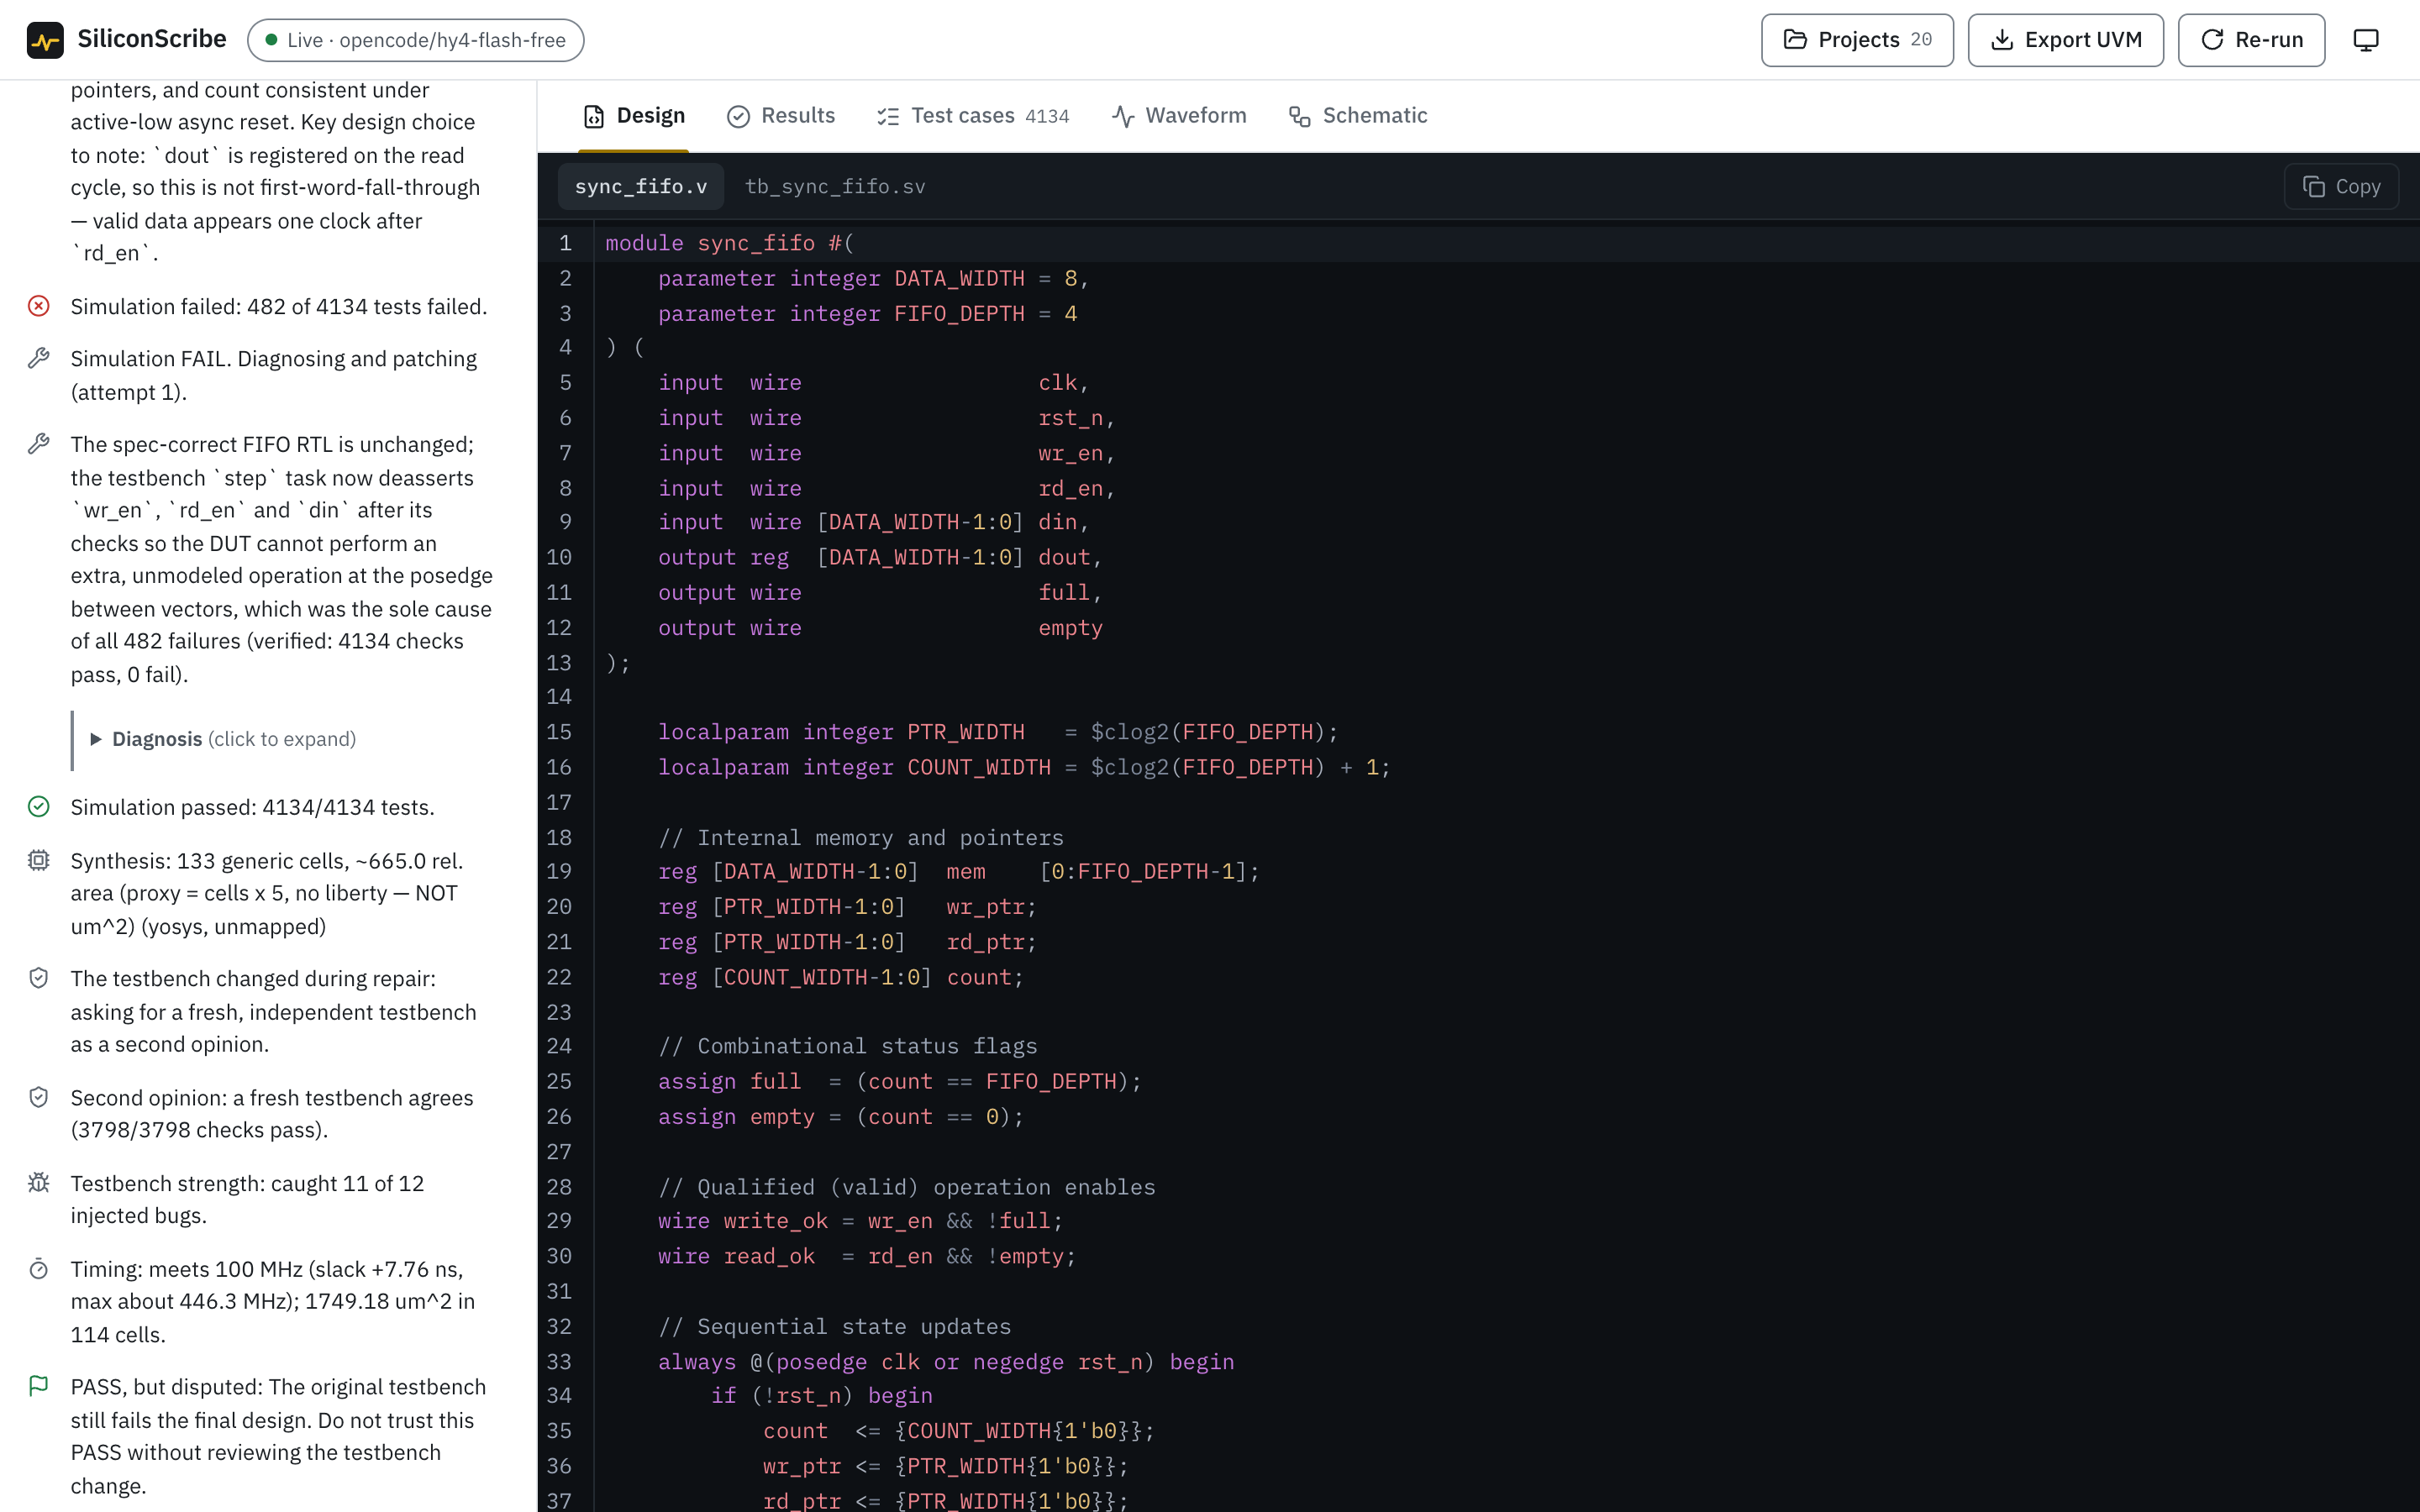
\includegraphics[width=0.92\textwidth]{s12_design_tab.png}
\caption{The Design tab: generated RTL and testbench in editable code editors.}
\end{figure}

\section{Editing and re-running}

You can edit the RTL or testbench directly in the Design tab, then press \textbf{Re-run} to simulate once more without the AI. This is useful for trying your own fix, or for checking that a deliberate bug is caught: change \code{count + 1'b1} to \code{count + 2'd2} in a counter, press Re-run, and the Test cases and Waveform tabs show the failures at once. Re-run clears strength, timing, the second opinion and ``Written by'', because those described the previous code.

\begin{figure}[H]
\centering
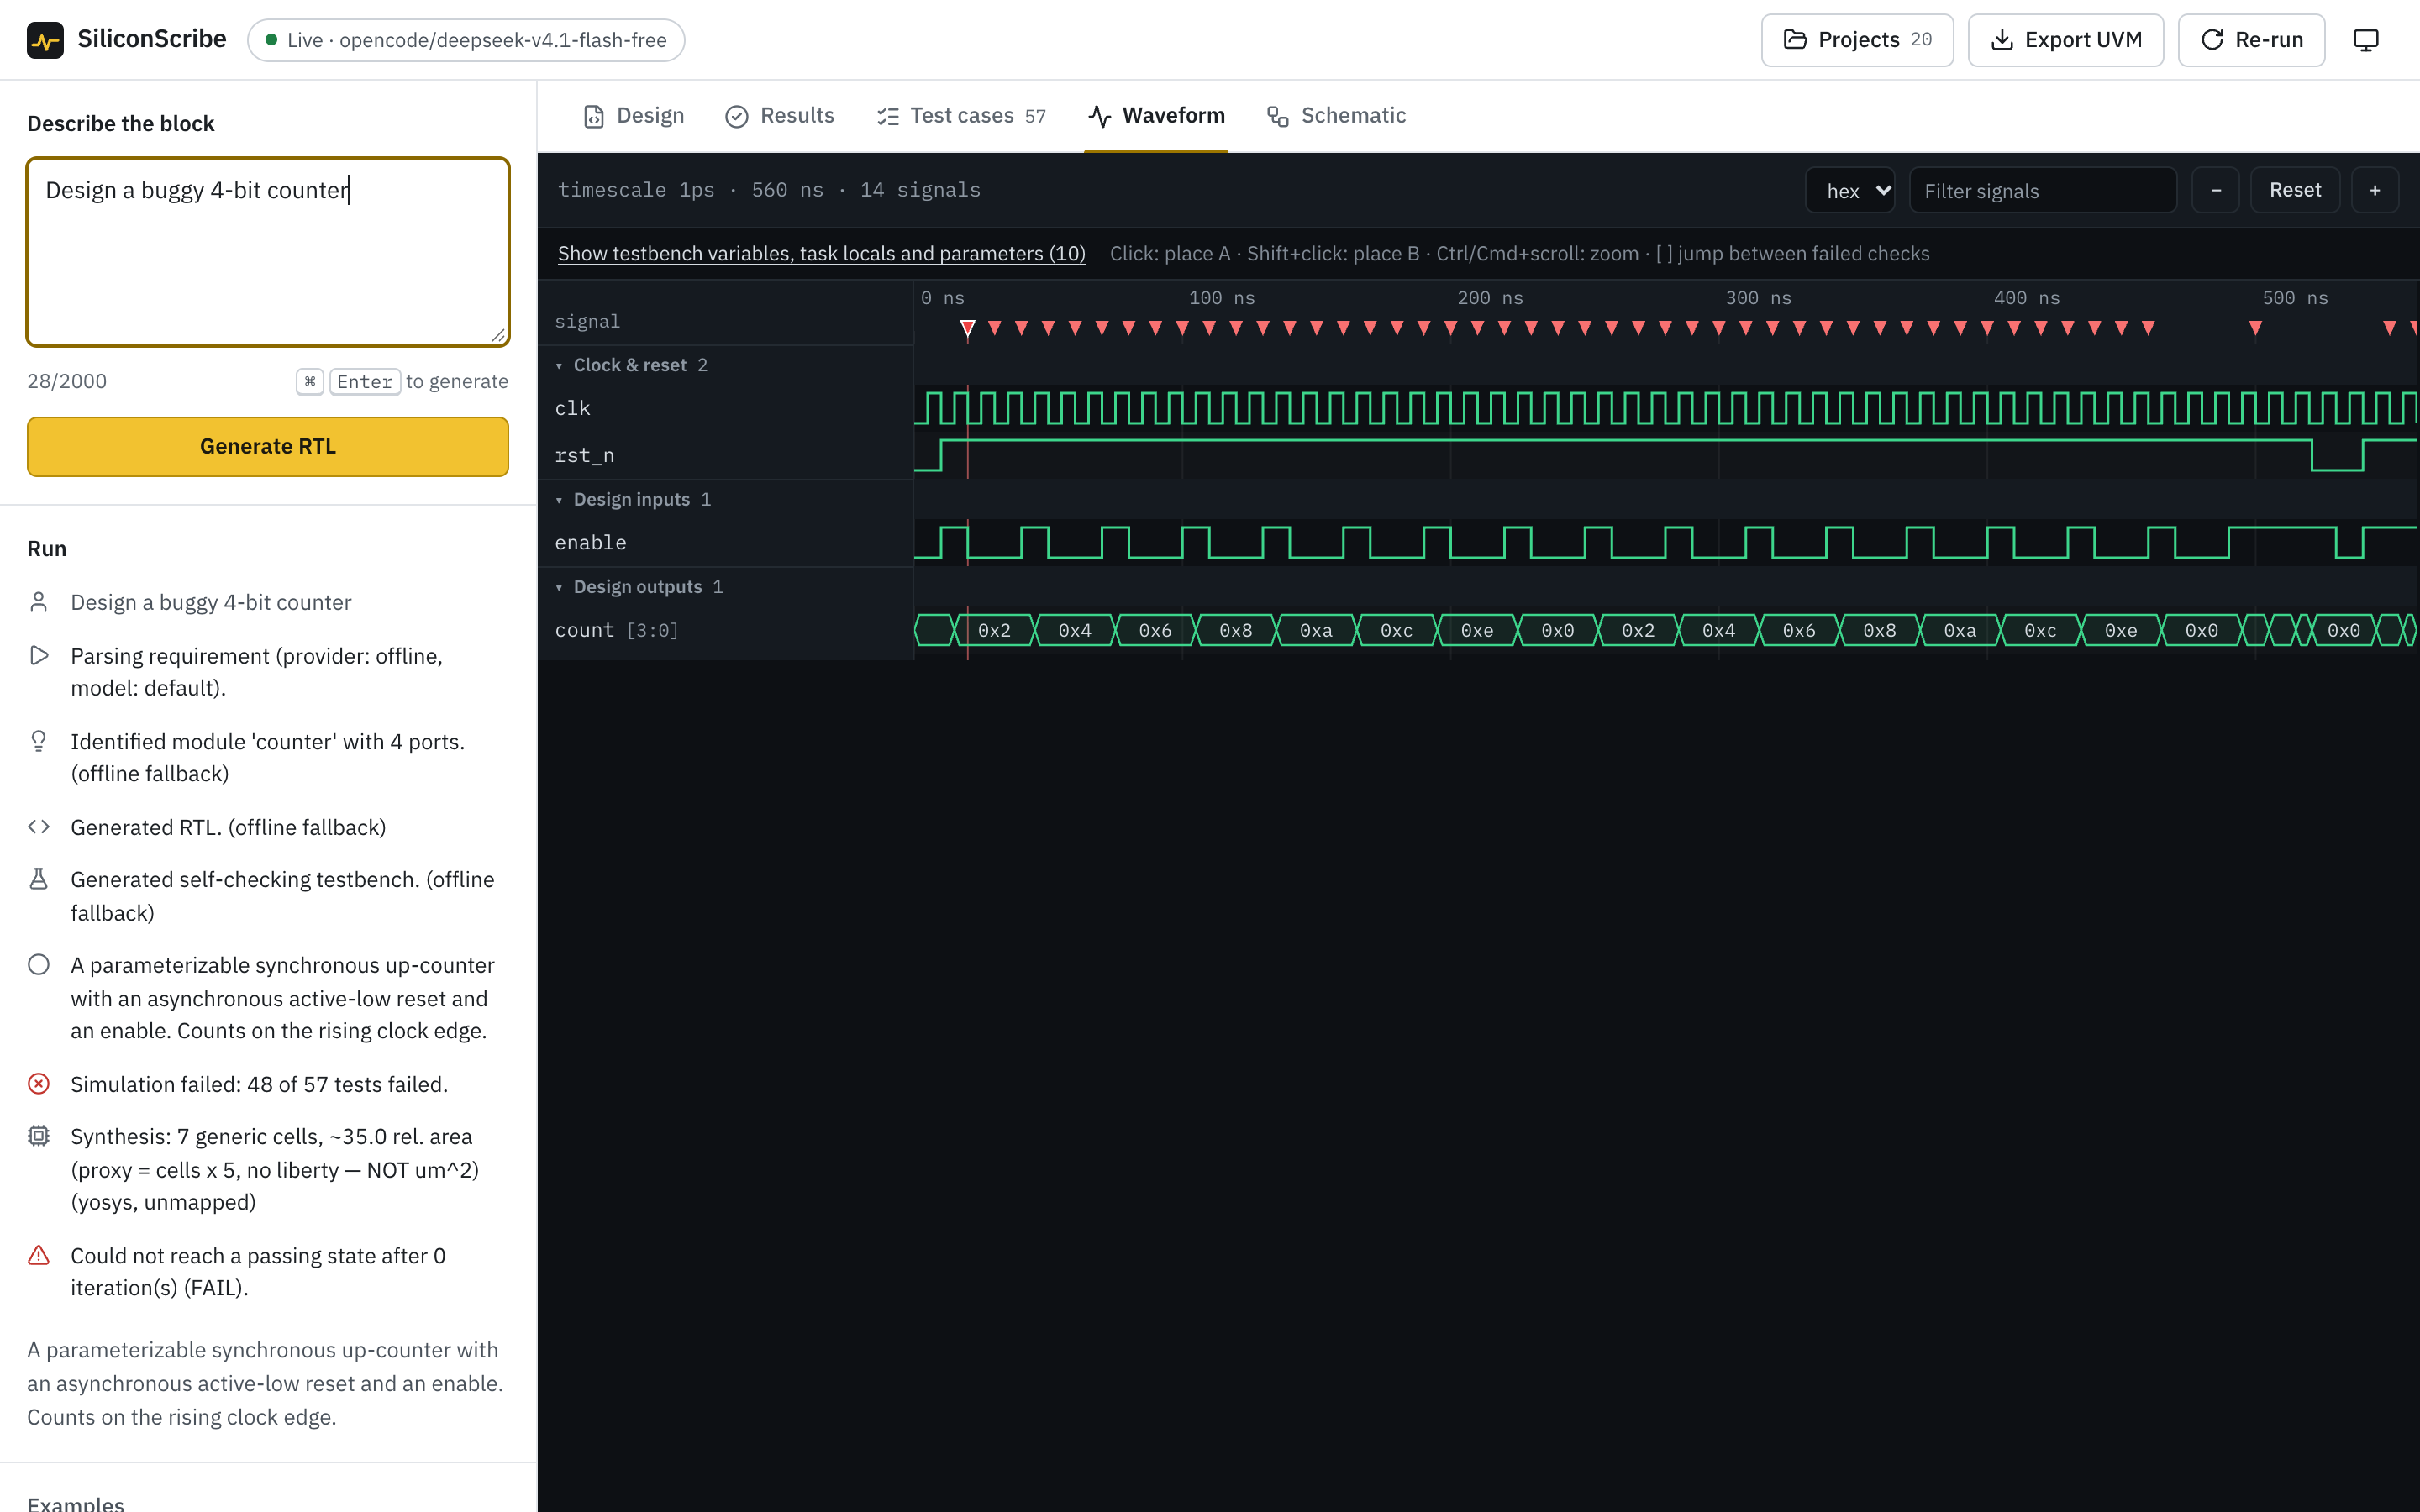
\includegraphics[width=0.92\textwidth]{s13_failure_waveform.png}
\caption{Waveform of the scripted buggy-counter demo (offline): each red marker is a failed check (48 of 57).}
\end{figure}

\section{Projects, theme, UVM export and Stop}

\textbf{Projects} opens a menu of saved runs (newest first), each with its module name, status and prompt, and \textbf{Open} and \textbf{Delete} buttons (Delete asks first). Before the first run, the start screen also lists recent projects. The theme button cycles between system (follows the computer's setting), light and dark; an explicit choice is remembered in the browser. \textbf{Export UVM} downloads the 16-file UVM bundle as a zip (export only: it is not simulated). \textbf{Stop} cancels a running generation.

\begin{figure}[H]
\centering
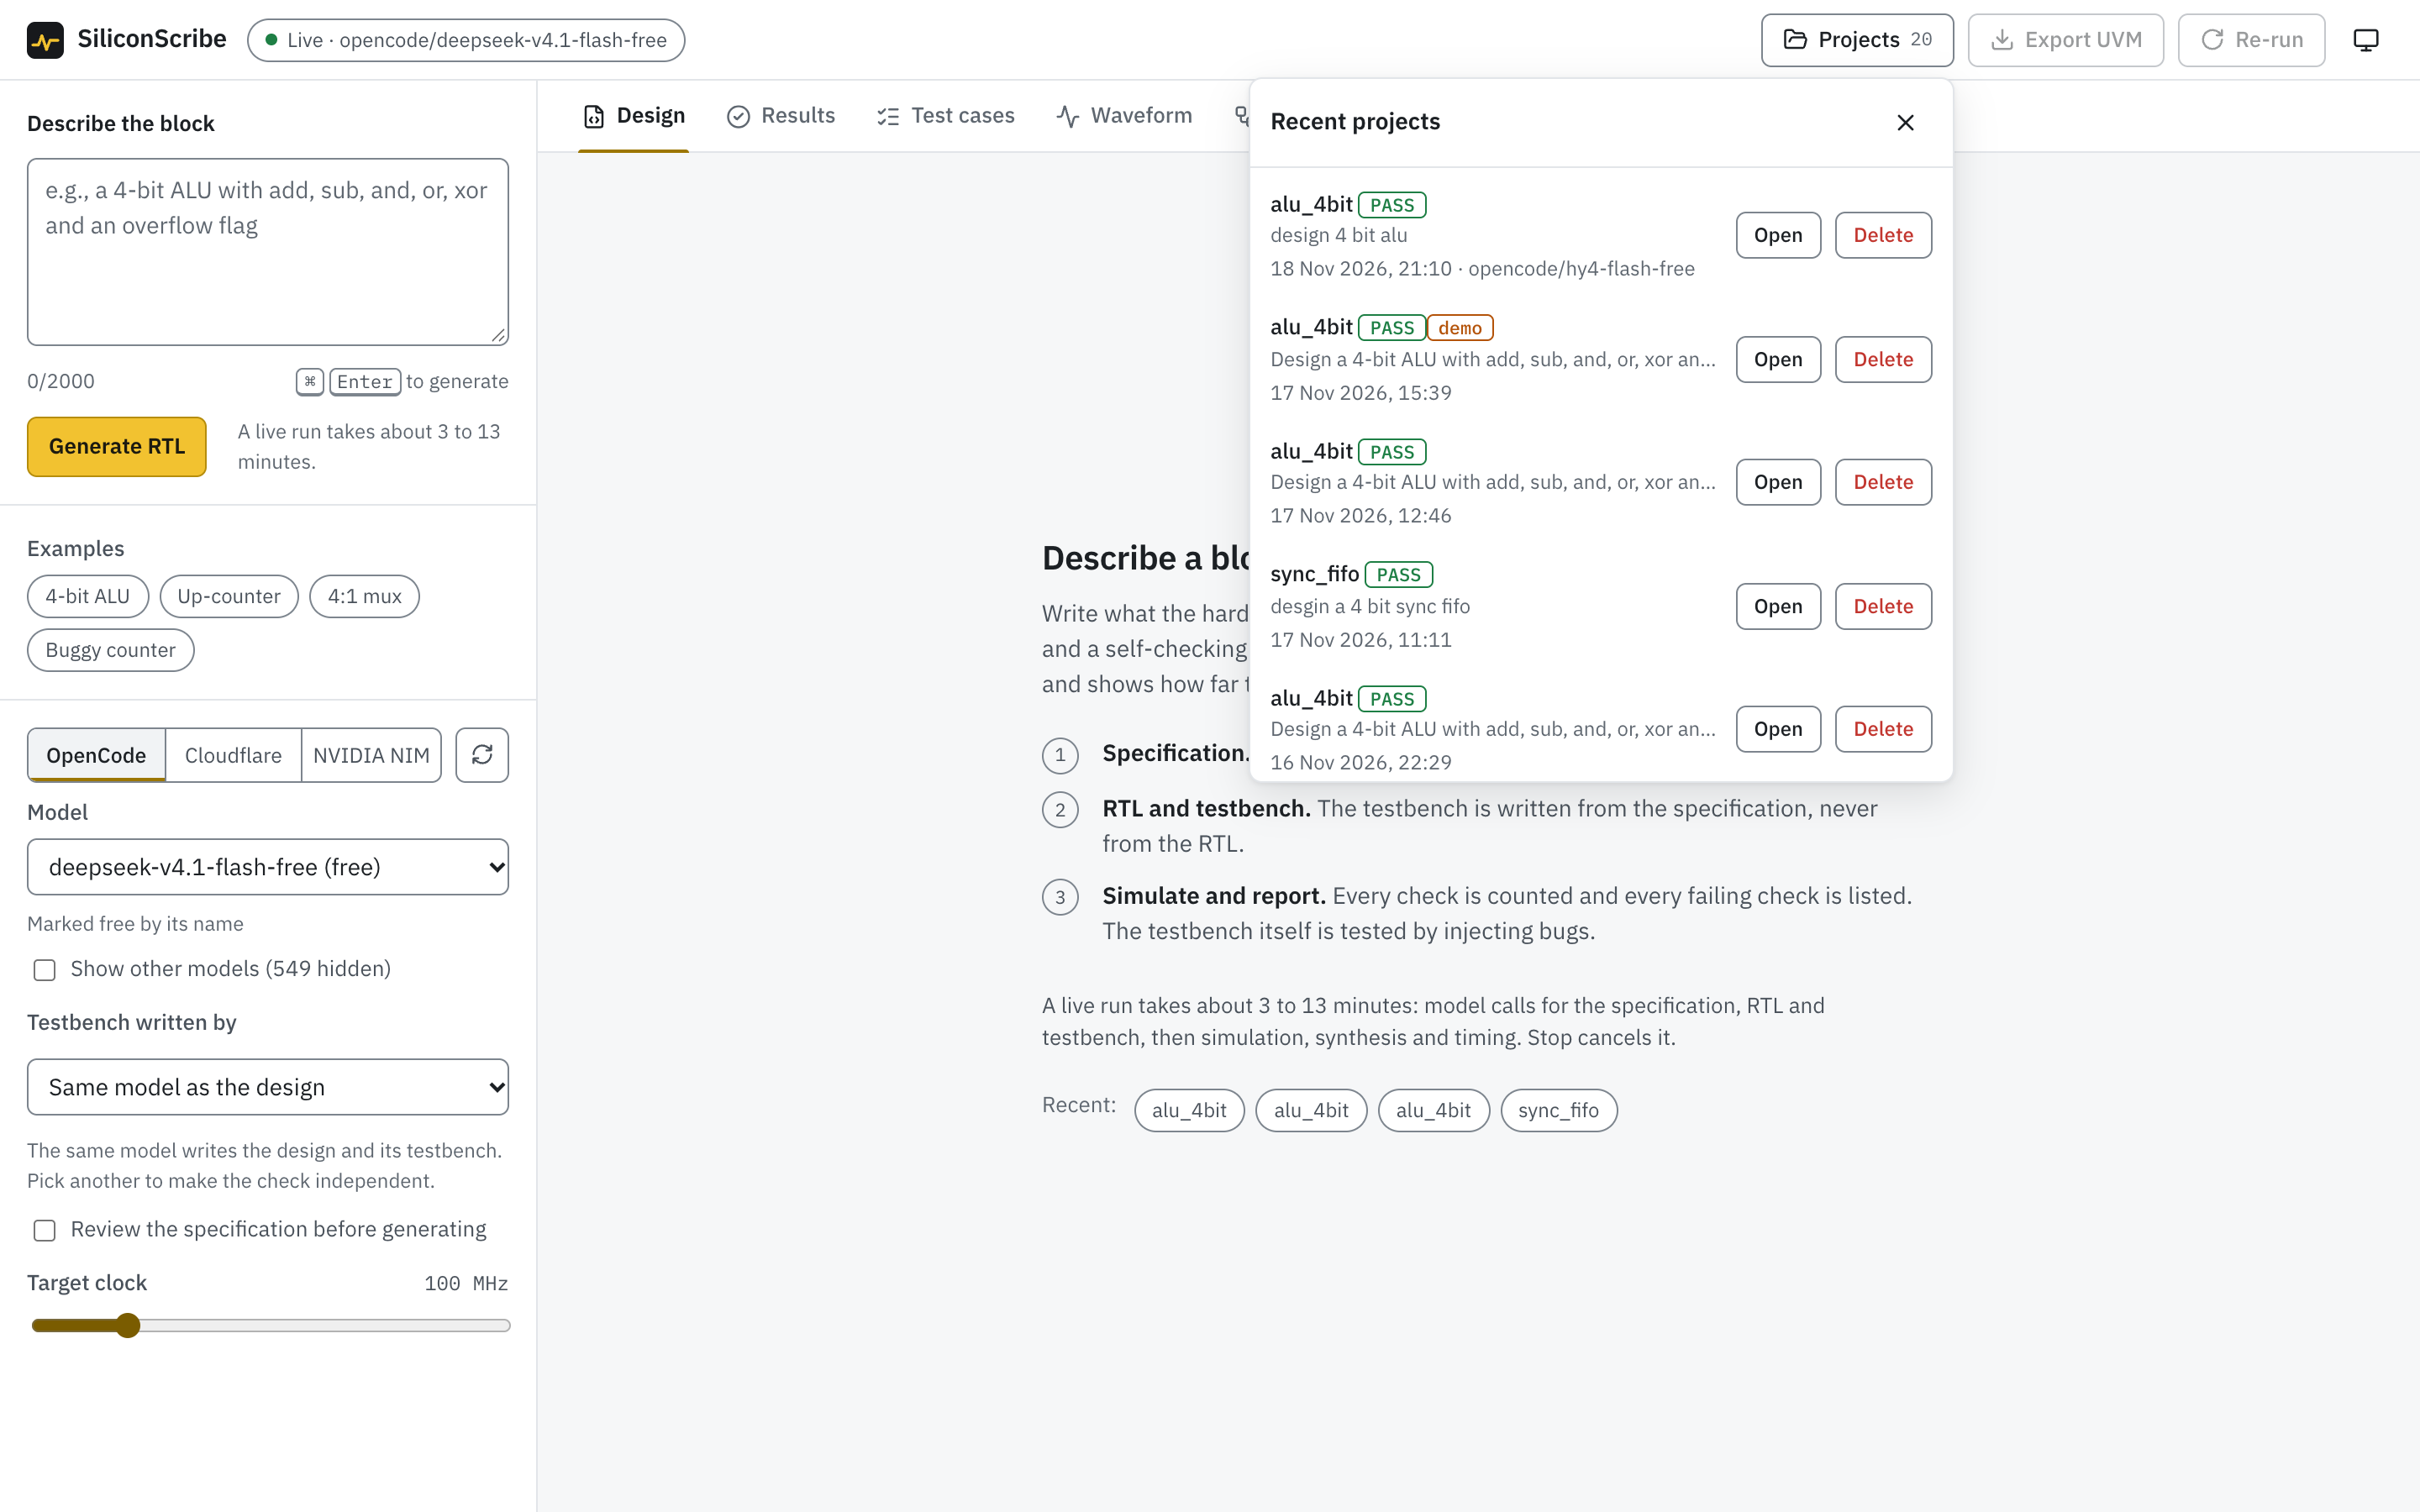
\includegraphics[width=0.92\textwidth]{s14_projects_menu.png}
\caption{The Projects menu listing saved runs.}
\end{figure}

\begin{figure}[H]
\centering
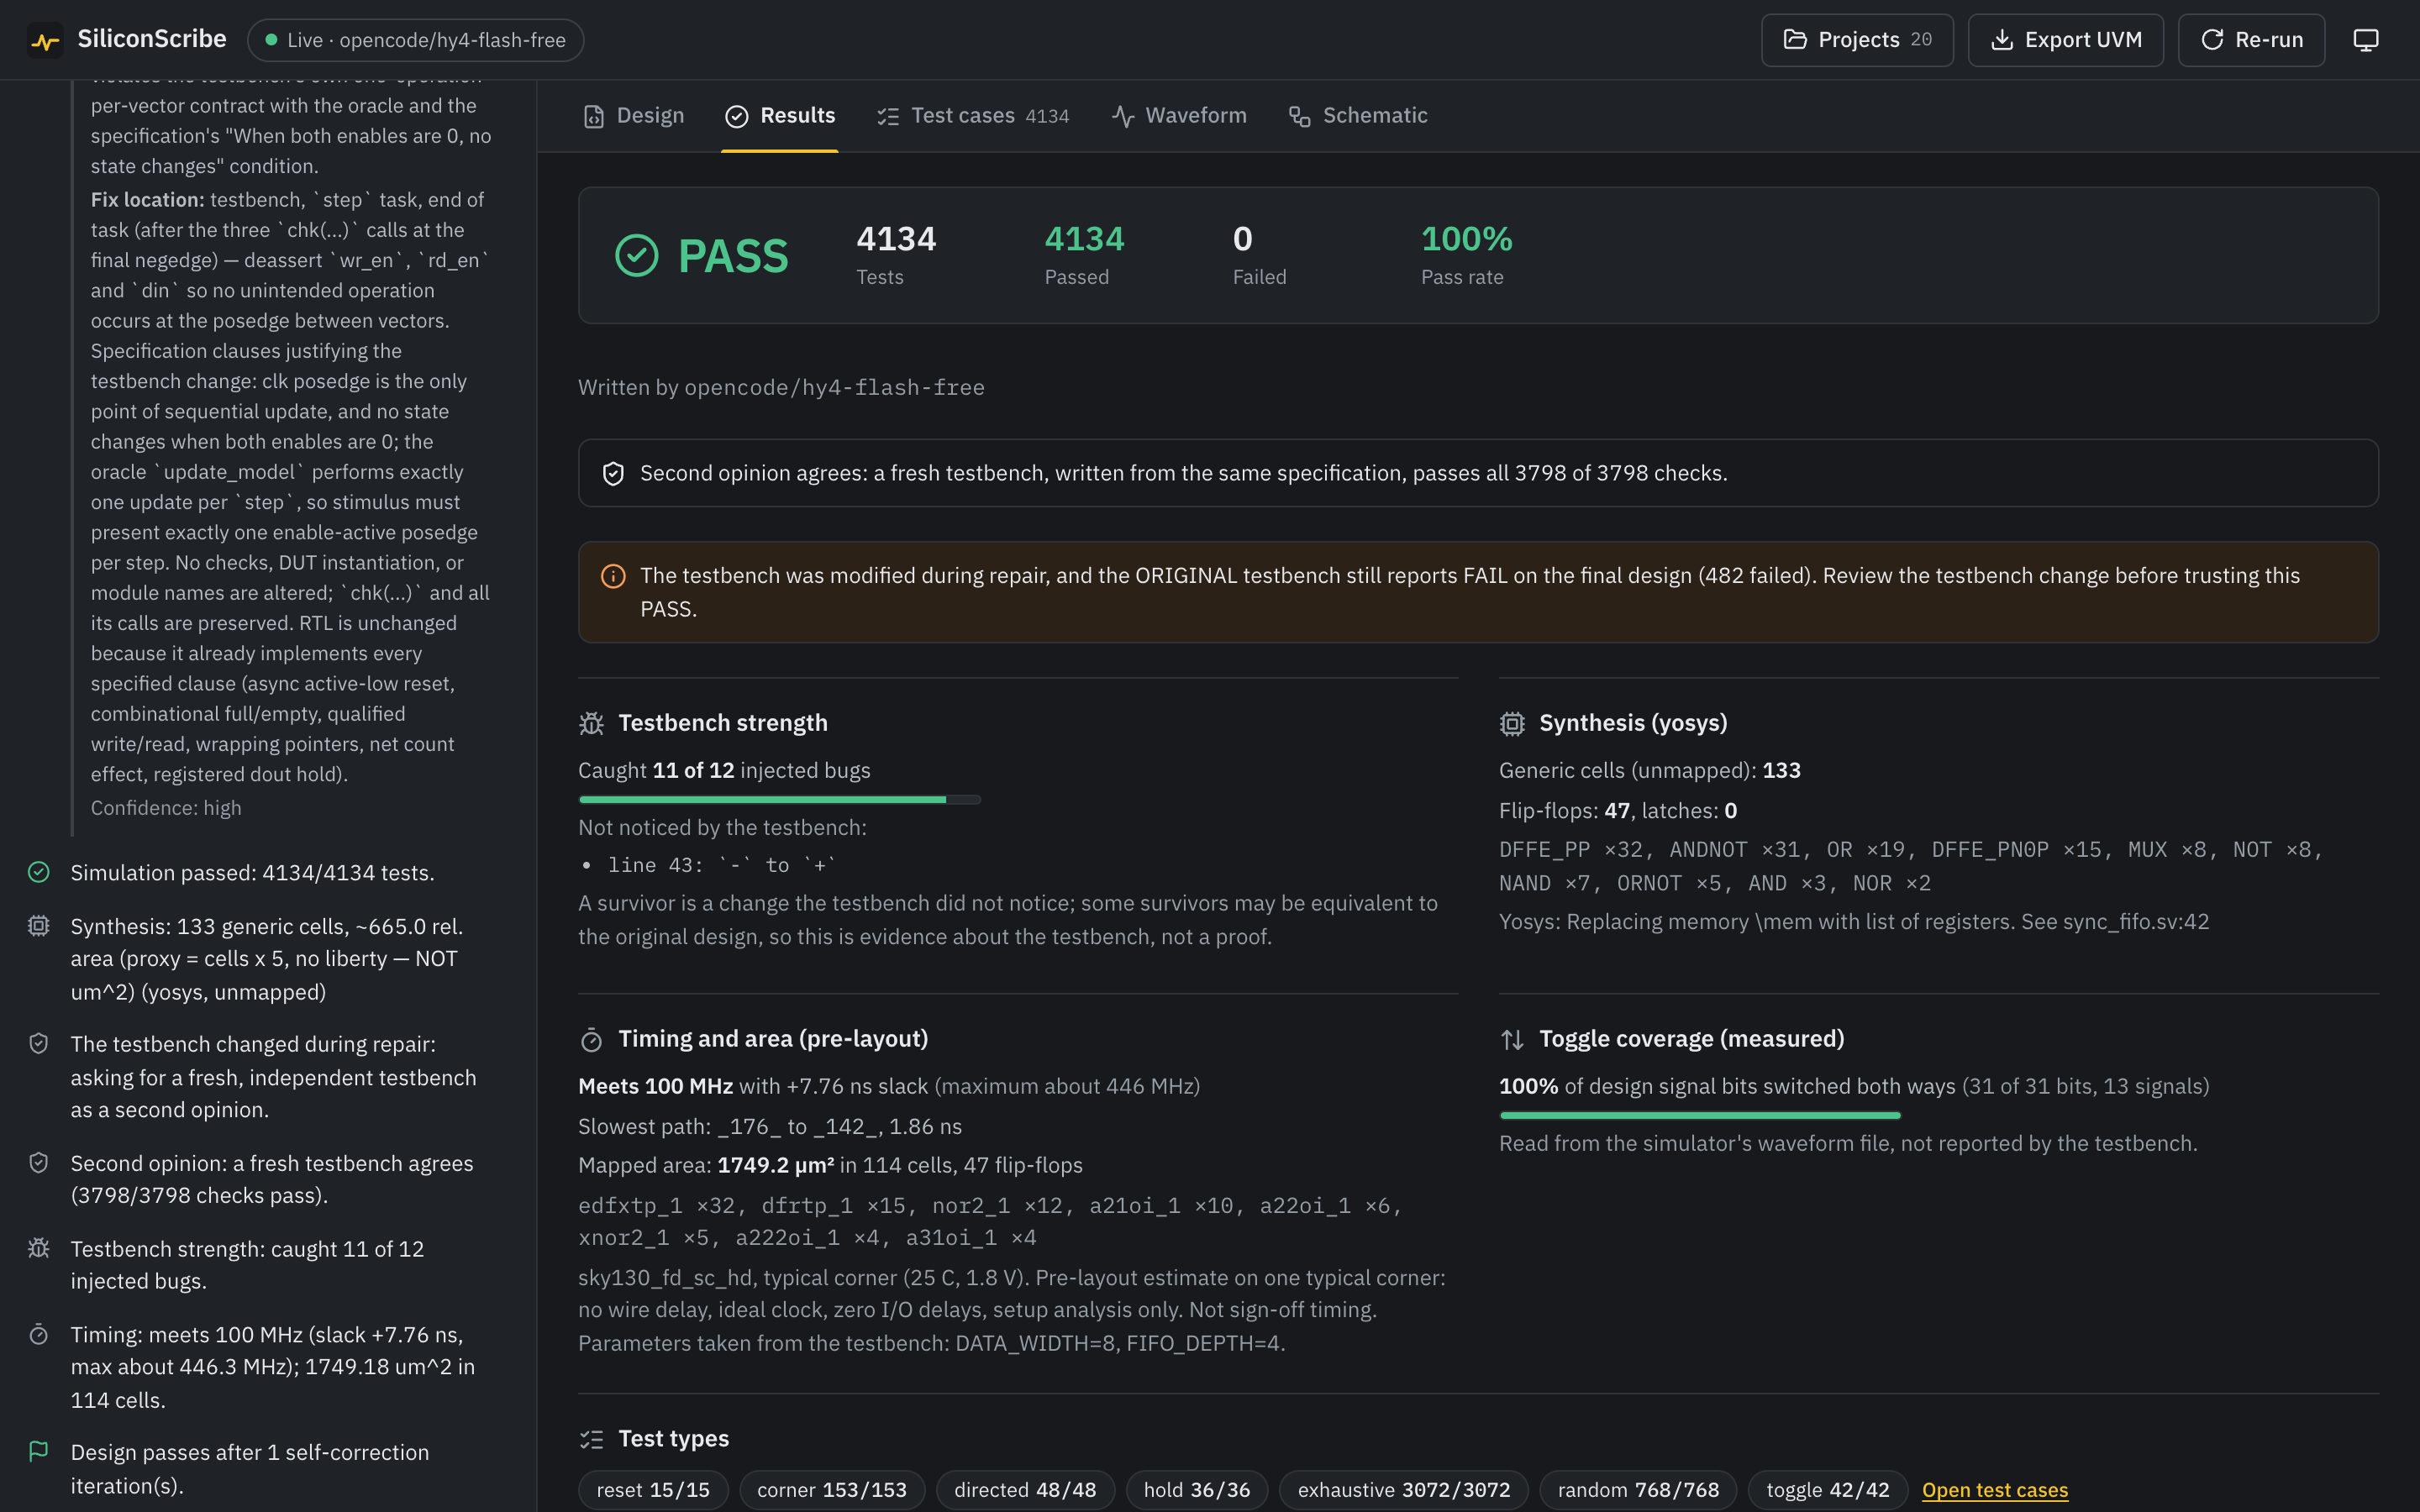
\includegraphics[width=0.92\textwidth]{s16_dark_theme.png}
\caption{The Results tab in the dark theme.}
\end{figure}

\begin{figure}[H]
\centering
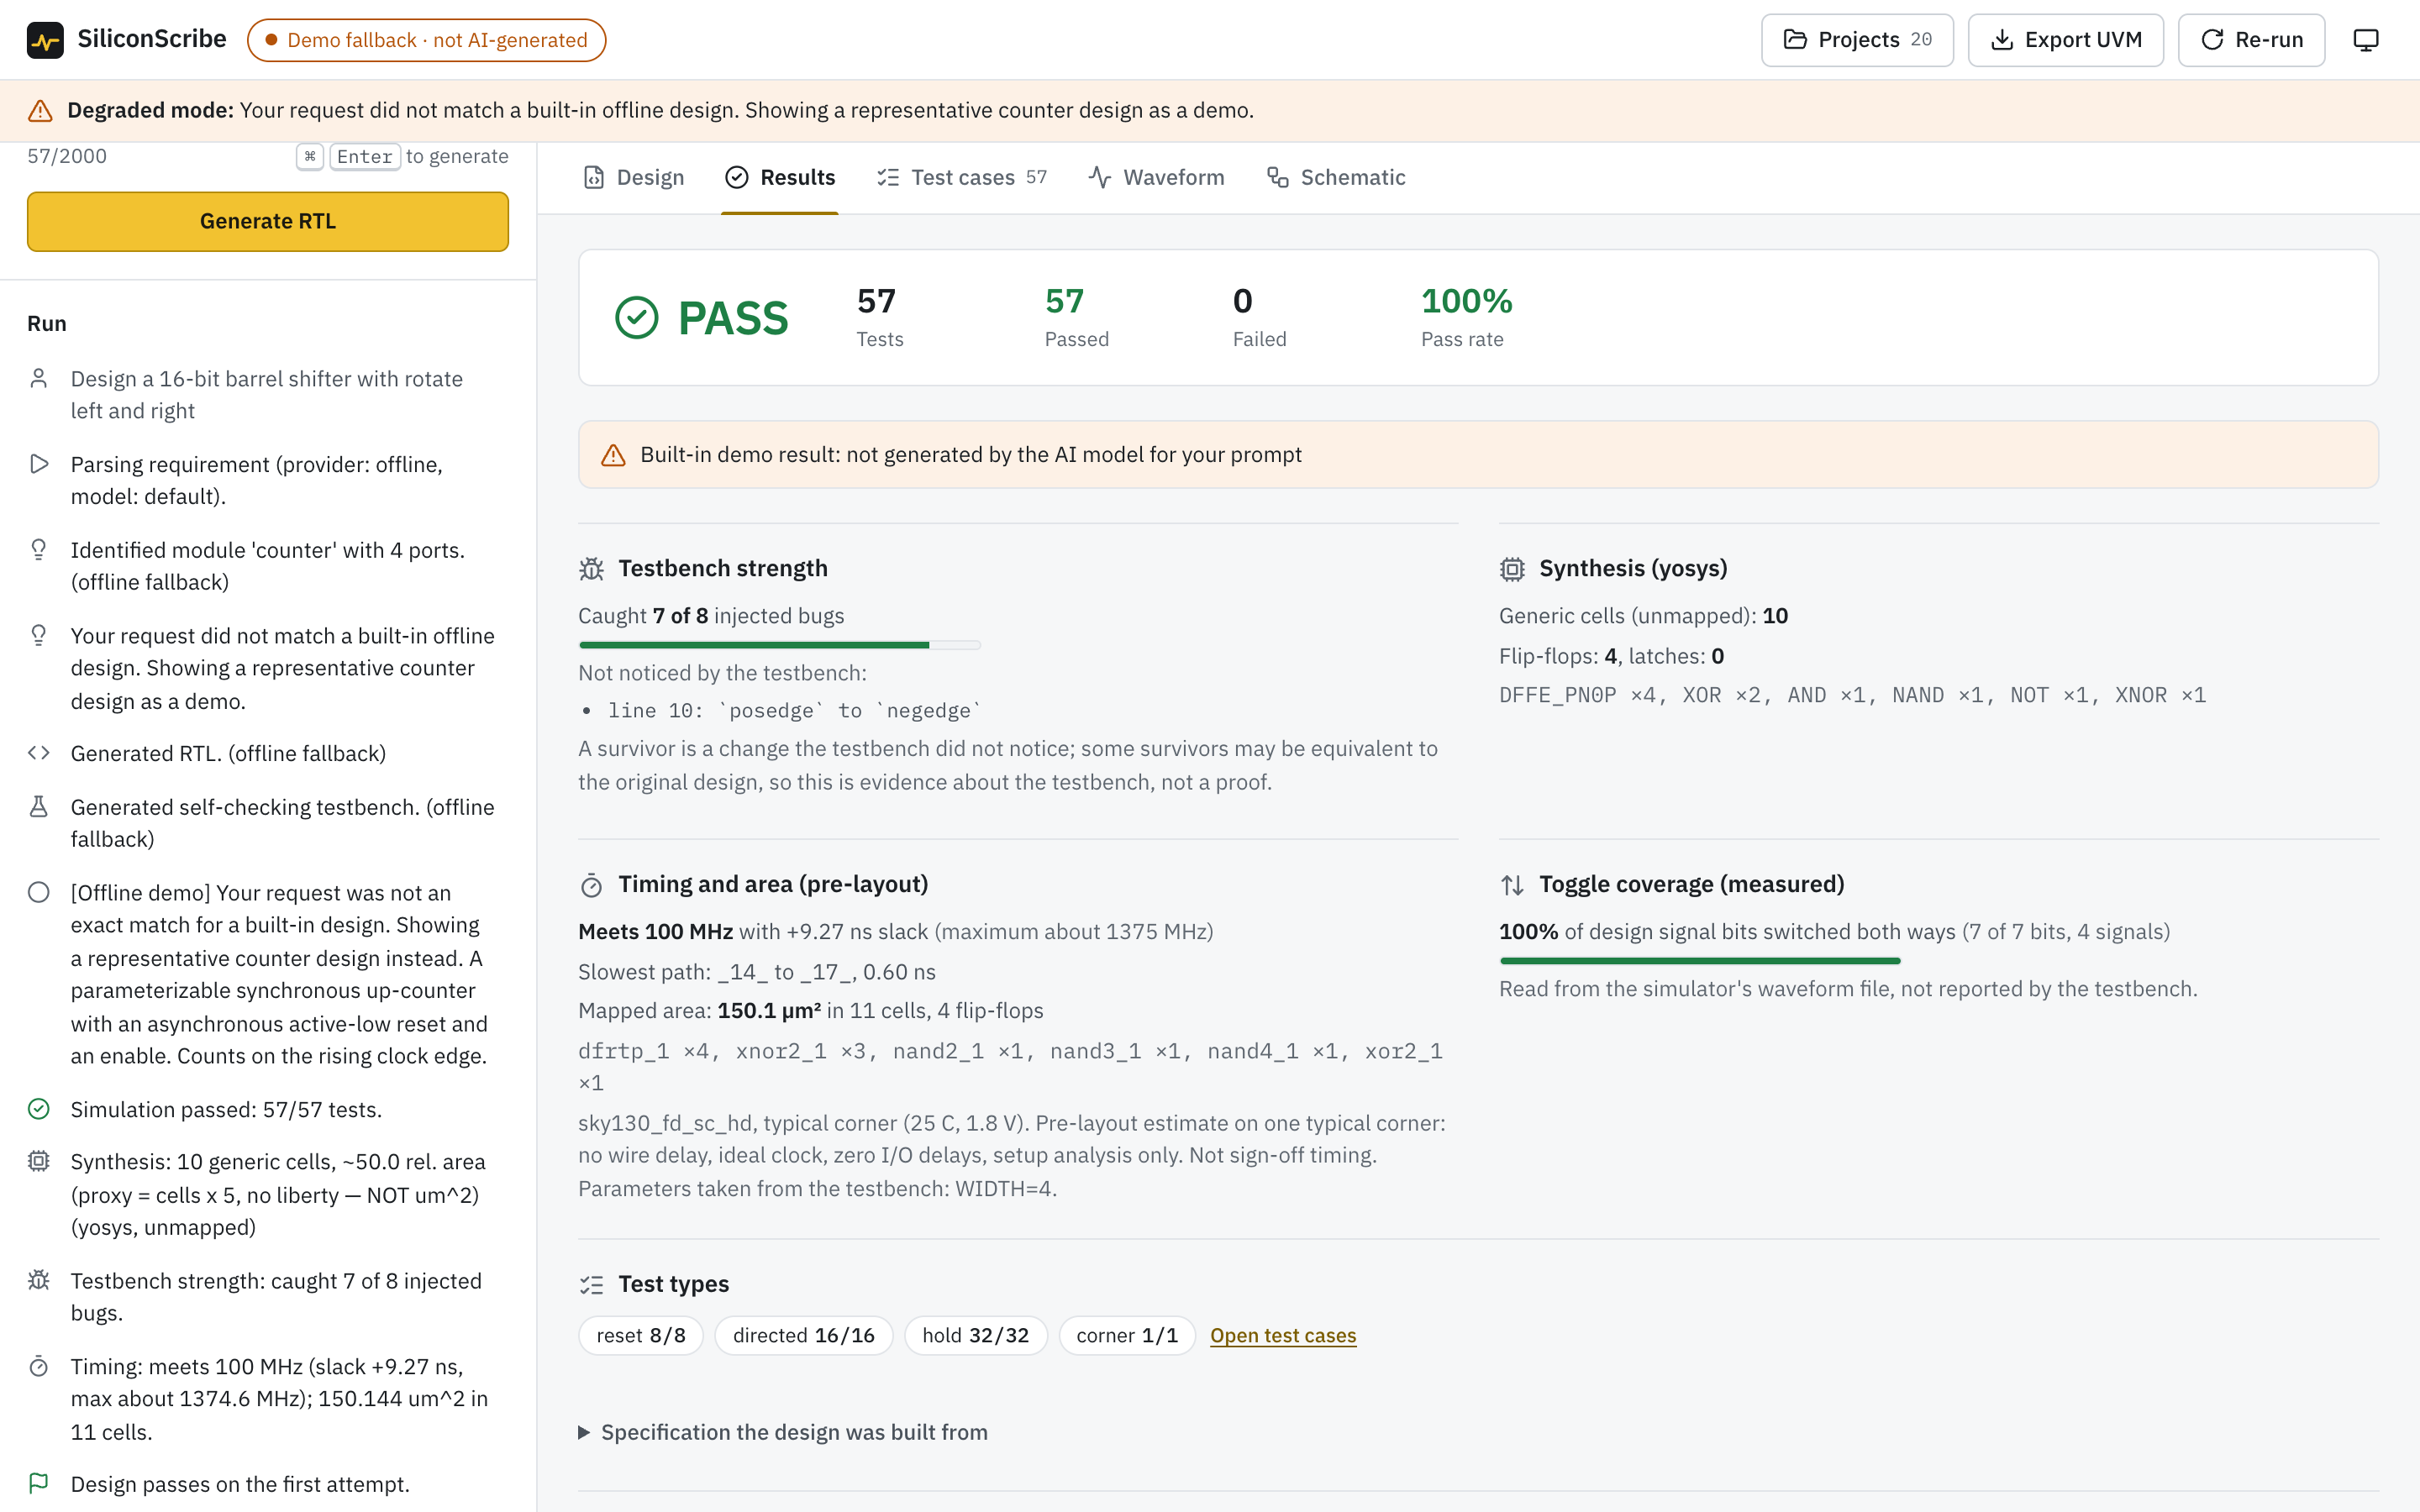
\includegraphics[width=0.92\textwidth]{s15_offline_demo.png}
\caption{A run that fell back to the built-in demo is labelled as such: the ``Degraded mode'' banner and ``Built-in demo result: not generated by the AI model for your prompt''.}
\end{figure}

% ---------------------------------------------------------------------------
\chapter{Testing and Quality}
\label{ch:testing}

\section{Verification commands}

These are the checks behind the numbers in this guide (final run: 19 Nov 2026). Run them from the project folder; none of them needs a key except the last.

\begin{lstlisting}[style=plain]
cd backend
PATH="$HOME/.local/bin:$PATH" OFFLINE_MODE=1 python3 -m pytest tests/ -q   # 436 passed
python3 tools/mutation_sweep.py                       # 27 of 27 injected bugs caught
PATH="$HOME/.local/bin:$PATH" python3 tools/verify_mapping.py   # 19 of 19 equivalent
python3 evaluation/independent/run.py                 # every evaluated design vs. its reference
PATH="$HOME/.local/bin:$PATH" python3 evaluation/independent/strength.py   # the references' own strength

cd ../frontend
npm test                                              # 211 passed (Vitest)
npm run build                                         # TypeScript check + production build
\end{lstlisting}

\begin{description}
  \item[pytest] 436 backend tests in 31 test files. They use a temporary workspace (the \code{_isolated_workspace} fixture in \file{tests/conftest.py}), so they never touch your real \file{projects.db}. Tests that need Icarus, Yosys or OpenSTA are skipped automatically if the tool is missing; Cloudflare and NIM are tested against small fake servers, not the internet.
  \item[Mutation sweep] Injects 27 known bugs into the built-in designs and checks that the built-in testbenches catch every one.
  \item[Mapping verification] The checks of Chapter~\ref{ch:timing}: gate-level simulation agrees with the RTL, area and cells recount, minimum period independent of the target. Each design says OK or REFUSED (with a reason).
  \item[Independent references] Hand-written reference testbenches, not written by any model, for the 14 evaluated designs. All 14 final designs were correct (no false PASS). \file{strength.py} runs \emph{every} mutant (not a sample of 12) against each reference; the references caught every mutant except equivalent ones, unreachable code, or behaviour the prompt does not define.
  \item[Frontend] 211 Vitest tests; \code{npm run build} runs the TypeScript compiler (clean) and the production build.
  \item[Accessibility] An automated axe-core audit of every tab, both themes, for a passing and a failing run: 0 violations. Its structural rules also run in the test suite. This is an automated audit, not a user study.
  \item[Tests of the tests] The newest components were broken on purpose, one behaviour at a time, and the tests had to fail.
\end{description}

\section{The preflight check}

Before a demo, \file{tools/preflight.py} checks everything the demo needs: the tools and their versions, the cell library, the model, the offline demo and the saved results. Each line is OK, WARN or FAIL, and the last lines say which rung of the fallback ladder (live model, offline demo, saved results) is usable. Without \code{--live} it makes no model call; with \code{--live} it makes one tiny call. It never writes to the projects database.

\begin{lstlisting}[style=plain]
cd backend
PATH="$HOME/.local/bin:$PATH" env -u OFFLINE_MODE LLM_PROVIDER=opencode-app \
  LLM_MODEL=deepseek-v4.1-flash-free LLM_TIMEOUT_SECONDS=360 python3 tools/preflight.py --live
\end{lstlisting}

The final run reported 0 failures and 0 warnings, with all three fallback rungs ready.

\section{What the test files protect}

\begin{center}
\small
\begin{tabularx}{\textwidth}{@{}>{\raggedright\arraybackslash}p{5.2cm}X@{}}
\toprule
\textbf{File(s)} & \textbf{Guards against} \\
\midrule
\file{test_orchestrator.py}, \file{test_edge_cases.py} & Broken repair loop, fallback rules, guards (anti-cheat, no-op, oscillation), compiler repairs, odd inputs. \\
\file{test_verdict_integrity.py}, \file{test_simulator.py} & A wrong verdict: misplaced or non-numeric summaries, zero checks, FAIL lines under ``Failed: 0'', killed runs, forged summaries in the RTL, system tasks not on the allow-list, narrow testbench wires, hangs. \\
\file{test_sandbox.py} & File access from Verilog, string tricks, the real exploit, environment scrubbing, output cap. \\
\file{test_verification_quality.py}, \file{test_mutation.py} & Testbenches that cannot fail; the strength stage (operators, protected regions, scoring, time budget). \\
\file{test_trust_signals.py}, \file{test_toggle_coverage.py} & The weak-evidence and weak-testbench warnings; measured toggle coverage. \\
\file{test_independent_testbench.py}, \file{test_spec_review.py} & The separate testbench model rules, the second opinion, the reviewed specification and its bounds. \\
\file{test_timing.py}, \file{test_verify_mapping.py}, \file{test_synthesis_metrics.py}, \file{test_yosys_warnings.py} & The timing stage (parsing, parameter overrides, clocks from the netlist, every refusal) and its checker; generic synthesis metrics; Yosys warnings shown with file names only. \\
\file{test_model_catalog.py}, \file{test_model_switching.py}, \file{test_model_routing.py}, \file{test_opencode_provider.py} & The Model menu, per-run model choice and routing, model-id validation, keys never leaking, the OpenCode app provider. \\
\file{test_llm_parsing.py}, \file{test_error_messages.py} & Fragile parsing of model answers; plain, safe error messages. \\
\file{test_api.py}, \file{test_stream_persistence.py}, \file{test_disconnect.py} & Routes, streaming, rate limit, saving streamed runs, a closed browser tab stopping further stages. \\
\file{test_check_parser.py}, \file{test_vcd_parser.py}, \file{test_vcd_roles.py}, \file{test_linter.py}, \file{test_models.py} & Check rows, waveform parsing and signal roles, lint, data shapes. \\
\file{test_preflight.py}, \file{test_evaluate_live.py} & The demo preflight and the live-evaluation recorder. \\
\bottomrule
\end{tabularx}
\end{center}

\begin{keyidea}
The most important tests are the ones that prove a check can fail: mutation tests of the testbenches, sabotaged netlists for the timing checker, broken components for the test suite itself. A test suite that only checks that correct designs pass proves very little.
\end{keyidea}

% ---------------------------------------------------------------------------
\chapter{Configuration Reference}
\label{ch:config}

All of these are read by the backend, from \file{backend/.env} or the environment.

\begin{center}
\small
\begin{longtable}{@{}>{\ttfamily\raggedright\arraybackslash}p{5.0cm}p{10.0cm}@{}}
\toprule
\textrm{\textbf{Variable}} & \textbf{Effect} \\ \midrule \endhead
OFFLINE\_MODE & 1/true/yes/on forces the offline provider. \\
LLM\_PROVIDER & \code{opencode-app}: use the installed OpenCode app. \\
LLM\_MODEL & Default model (where the Model menu starts), for example \code{deepseek-v4.1-flash-free}. \\
OPENCODE\_AGENT & OpenCode agent used for each call (default \code{plan}, read-only). \\
CLOUDFLARE\_ACCOUNT\_ID, CLOUDFLARE\_API\_TOKEN & Turn on the Cloudflare tab. \\
NVIDIA\_NIM\_API\_KEY, NVIDIA\_NIM\_BASE\_URL & Turn on the NVIDIA NIM tab (key starts \code{nvapi-}). \\
OPENCODE\_API\_KEY / ZEN\_API\_KEY, ZEN\_MODEL, OPENCODE\_BASE\_URL & OpenCode Zen as the default provider instead of the app. \\
NVIDIA\_API\_KEY, NVIDIA\_BASE\_URL & Older single-model NVIDIA default provider (not used by the NIM tab). \\
OPENAI\_API\_KEY, OPENAI\_BASE\_URL, LLM\_MINI\_MODEL & OpenAI, or any compatible gateway when a base URL is given. \\
LLM\_MODEL\_INTENT, \_RTL, \_TESTBENCH, \_EXPLAIN, \_FIX & Per-stage model routing for the default provider (a model chosen in the menu still wins). \\
LLM\_TIMEOUT\_SECONDS & Per-call timeout (default 120; 360 for the free models in the demo). \\
LLM\_MAX\_TOKENS & Answer budget (default 8192). \\
STRENGTH\_ENABLED, STRENGTH\_MAX\_MUTANTS, STRENGTH\_BUDGET\_SECONDS & Testbench strength on/off (default on), mutants per run (12), time budget (40 s). \\
TIMING\_ENABLED & Timing and area estimate on/off (default on; needs the tools and library). \\
SECOND\_OPINION\_ENABLED & Second opinion on/off (default on). \\
SIM\_MAX\_CONCURRENT, SIM\_MAX\_MEMORY\_MB & Simulations at once (2); memory cap per simulation (1024 MB, Linux only). \\
CORS\_ALLOW\_ORIGINS & Extra exact browser origins allowed to call the API (comma-separated, no wildcards). \\
TRUST\_PROXY\_HEADERS & 1 only behind a trusted reverse proxy, so the rate limit uses the forwarded address. \\
ADMIN\_TOKEN & Enables \code{/api/admin/cleanup}; sent as the \code{X-Admin-Token} header. \\
VITE\_API\_BASE & Frontend: backend address if not served from the same origin. \\
\bottomrule
\end{longtable}
\end{center}

% ---------------------------------------------------------------------------
\chapter{Troubleshooting}
\label{ch:trouble}

\begin{center}
\small
\begin{longtable}{@{}p{4.6cm}p{10.4cm}@{}}
\toprule
\textbf{Symptom} & \textbf{Cause and fix} \\ \midrule \endhead
Status ERROR, ``Compilation failed'' & The code does not compile. Read the error line in the log; the loop repairs wire/reg and disable/return automatically and asks the model for anything else. \\
``Rejected by sandbox policy'' & The code uses a file or system task (\code{$fopen}, \code{$readmemh}, \code{`include}, \ldots) or a task not on the allow-list. Remove it. \\
Status ERROR, ``No valid summary'' & The testbench did not print whole-line \code{Passed:} and \code{Failed:} numbers, often because its own watchdog fired first. Re-run with a fresh testbench or another model. \\
``The model you chose (\ldots) could not be used'' & That model hit its limit, timed out, was refused or is unknown. Pick another model from the Model menu. Your run is not replaced by the demo. \\
``The AI model did not answer in time'' & Free models can take minutes per step. Try again, pick another model, or raise \code{LLM_TIMEOUT_SECONDS}. \\
``free usage limit has been reached'' & The free quota is used up; it resets daily. Switch model or provider, or use the offline demo or a saved project. \\
Cloudflare or NVIDIA NIM tab says ``not set up'' & The key is missing or malformed in \file{backend/.env}. Fix it and restart the backend. \\
Cloudflare HTTP 403, code 5035 & That model is not allowed on the Workers Free plan. Pick another. \\
GitHub Copilot is not in the menu & Connect it in the OpenCode app with \code{/connect}, press the refresh button, tick ``Show other models''. \\
``LLM became unavailable mid-run'' & The provider failed after the run had started producing your design. Retry; the app refuses to swap in a demo design at this point. \\
Banner ``Degraded mode'' & The default provider failed before anything was generated, so the run used built-in designs and says so. Check the model and network. \\
No ``Timing and area'' section & Yosys, OpenSTA or \file{backend/pdk/sky130hd_tt.lib} is missing, or the run did not PASS. Start the backend with \code{PATH="$HOME/.local/bin:$PATH"}. \\
Timing shows a reason instead of a number & The design has tri-states, latches, a combinational loop, a derived or gated clock, or no logic cells. This is a deliberate refusal (Chapter~\ref{ch:timing}). \\
HTTP 429 & More than 20 requests in a minute from your address. Wait a minute. \\
Status TIMEOUT & The testbench never calls \code{$finish}, or runs too long. Check loops; the limit is 1--120 s (30 s from the UI). \\
The browser cannot reach the API from another address & CORS allows local addresses only. Add the exact origin with \code{CORS_ALLOW_ORIGINS}. \\
\code{simulator: false} in /health & Icarus is not on the PATH. Install it and restart. \\
\bottomrule
\end{longtable}
\end{center}

% ---------------------------------------------------------------------------
\chapter{Extending the Project}
\label{ch:extend}

\section{Adding an LLM provider}
Any OpenAI-compatible service works as the default provider with no code change: set \code{OPENAI_API_KEY}, \code{OPENAI_BASE_URL} and \code{LLM_MODEL}. To add it as a tab of the Model menu (like Cloudflare and NIM), give its ids a unique prefix, add a \code{..._config}, a catalogue reader and a \code{..._status} function in \file{model_catalog.py} that read the key only from the environment and never return it, add a small subclass of \code{OpenAIProvider} in \file{llm_service.py}, route the prefix in \code{get_provider}, add it to \code{list_models}, and add a fake server for its tests. Keep every id inside \code{MODEL_ID_RE}.

\section{Adding a built-in design}
In \file{offline_designs.py}, add a spec, an RTL string starting with \code{_marker("key")}, a self-checking testbench ending with the summary lines, and an explanation; register it in \code{DESIGNS} and add keywords to \code{_KEYWORDS}. Then add mutants for it in \file{tests/test_verification_quality.py} and \file{tools/mutation_sweep.py} to prove its testbench can fail, and run \file{tools/verify_mapping.py} on it.

\section{Adding a compiler repair}
Write a function like \code{_repair_disable_functions} that only acts when the compiler log contains a specific, unambiguous message, call it from \code{_compiler_repairs}, return a structured diagnosis, and add a test with the real compiler message.

\section{Adding a pipeline stage or UI panel}
Yield a new event from \code{pipeline_events} with its own \code{stage} name, add the stage to \code{StreamEvent} in \file{frontend/src/types.ts}, handle it in \code{startRun}, and render it in a component. Keep extra stages non-fatal, as the explanation, strength, timing and second-opinion stages are.

% ---------------------------------------------------------------------------
\chapter{Why It Is Built This Way}
\label{ch:why}

\begin{description}[style=nextline]
  \item[Why generate the testbench from the specification and not the RTL?]
  So a wrong design and its testbench cannot simply agree. It removes the most direct form of circular checking.
  \item[Why offer a separate testbench model, but not by default?]
  Two models reading the specification independently can catch a misreading one model would make twice. But it costs an extra call, and with the free models tried it was not reliable enough to be the default. As an option it makes disagreements visible instead of quietly repaired.
  \item[Why a second opinion after a repair?]
  A PASS that appears only after the testbench was rewritten might come from a relaxed check. A fresh testbench from the same specification is cheap independent evidence; disagreement is the signal.
  \item[Why measure testbench strength on every PASS?]
  A PASS from a testbench that cannot catch bugs means little. Injecting small bugs and counting how many are caught is the classic, direct way to ask.
  \item[Why only toggle coverage?]
  It can be measured honestly from the VCD the simulator already writes. Line and branch coverage need a simulator that instruments the code; Verilator was tried and could not build most of the generated testbenches.
  \item[Why Icarus Verilog and not a commercial simulator?]
  It is free, open source, scriptable and installable anywhere, which fits a zero-budget project. The trade-off is limited SystemVerilog support (hence the Icarus-safe prompts and repairs, and why UVM is export-only).
  \item[Why a pre-layout timing estimate and not final timing?]
  Sign-off needs place and route, extracted wire delays, a real clock tree and several corners. That is a full physical-design flow. A pre-layout estimate on real sky130 cells already answers the useful early question, and every limit is printed next to the number.
  \item[Why refuse some designs instead of timing them?]
  For tri-states, latches, loops and derived clocks this simple set-up would time a different circuit or an undefined one. A reason is honest; a number would not be.
  \item[Why fix compiler errors without the AI?]
  When the compiler names the exact problem, the fix is mechanical. A deterministic repair is instant, free and always correct for that case; the AI is kept for real reasoning.
  \item[Why read model catalogues live?]
  Model names change and models are retired (one NIM model returned HTTP 410 three days before the final check). A hand-written list goes stale.
  \item[Why keep keys only in \texttt{backend/.env}?]
  A key typed into a web page can leak through the browser, logs or screenshots. The backend is the only part that needs it.
  \item[Why Server-Sent Events and not WebSockets?]
  The data only flows one way (server to browser) during a run. SSE is plain HTTP, works through proxies and hosting platforms, and needs no extra protocol.
  \item[Why SQLite?]
  Zero setup and zero cost for a single server. The report's scaling path moves to PostgreSQL for many users.
  \item[Why disable hidden reasoning by default?]
  Reasoning tokens use the same budget as the answer. In a live test a model spent all 8192 tokens thinking and returned nothing.
  \item[Why fall back to offline only before the first live success, and never for a model you chose?]
  Before anything is generated, a labelled demo is better than an error. After your design exists, or when you deliberately picked a model, swapping in a demo would be dishonest, so the run fails with a plain reason instead.
  \item[Why plain \texttt{def} handlers instead of \texttt{async def}?]
  Simulations block while waiting for a subprocess. In \code{async def} they froze the whole server; in \code{def} FastAPI runs them in a thread pool.
\end{description}

\section{Limitations to state openly}

\begin{enumerate}
  \item One model writes the design and the testbench unless a separate testbench model is chosen (common-mode risk).
  \item The specification is written by the model unless you review it.
  \item Testbench strength is a sample of up to 12 one-token (syntactic) mutants; survivors may be equivalent.
  \item Only toggle coverage is measured; there is no line or branch coverage, no assertions and no formal checks.
  \item Timing is pre-layout on one typical corner: no wires, ideal clock, setup only, no power. It is not sign-off.
  \item Free models are slow (minutes per run) and quota-limited.
  \item The sandbox is defence in depth, not a jail or a container boundary.
  \item The evaluation used small blocks (under about 100 lines), one run per prompt, mainly one model.
  \item GitHub Copilot ``auto'' cannot name the model that wrote a result.
  \item The UVM bundle is exported, not compiled or run.
  \item One server, in-process rate limiter, SQLite, and a local single-user model provider: not a multi-user production service.
\end{enumerate}

\section{Future work}

\begin{enumerate}
  \item A multi-model comparison on the 15 prompts, with the reference check and strength per model.
  \item Assertions (SVA) and formal equivalence checking.
  \item Line and branch coverage with a simulator that supports the generated testbenches.
  \item Place and route with OpenROAD for post-layout timing.
  \item Container isolation and a job queue for multi-user use.
  \item Splitting the roughly 500-line pipeline function into smaller pieces.
\end{enumerate}

% ---------------------------------------------------------------------------
\chapter{Viva Question Bank}
\label{ch:vivaqa}

Short, honest answers you can give in your own words.

\begin{description}[style=nextline]
  \item[1. What does your project do, in one sentence?]
  It turns a plain-English hardware request into Verilog RTL and an independent self-checking testbench, runs them in a real simulator, repairs failures, and measures how much the PASS is worth; the simulator decides PASS or FAIL, never the model.
  \item[2. What is novel compared with just using ChatGPT?]
  The closed loop with a real simulator, the specification-derived testbench, structured diagnosis with deterministic compiler repairs, guards against test evasion, and the measurements around a PASS (strength, toggle coverage, second opinion, timing), all with honest labelling.
  \item[3. What is RTL?]
  Register-transfer level: describing hardware as registers and the logic between them, clock edge by clock edge, in a language such as Verilog.
  \item[4. What is a testbench? What is self-checking?]
  A Verilog module that drives the design's inputs and checks its outputs. Self-checking means it compares against expected values and prints a verdict itself.
  \item[5. How is PASS decided?]
  From the simulator transcript: the last whole-line \texttt{Passed:} and \texttt{Failed:} numbers. Failed above zero, or any FAIL/ERROR line, is FAIL; no valid summary, zero executed checks or a killed run is ERROR; otherwise PASS. Zero checks is never PASS.
  \item[6. Why can't the model just say it passed?]
  Because models predict text and can be wrong with confidence. Only execution is evidence, and even then PASS is evidence, not proof.
  \item[7. What happens when simulation fails?]
  If the compiler names a known mechanical error, it is repaired deterministically. Otherwise the model receives the spec, code and log, and must return a symptom, root cause, fix location, confidence and a minimal patch. The design is re-simulated, up to five times from the UI.
  \item[8. How do you stop the AI deleting tests to pass?]
  A fix that reduces the checks in a testbench that already ran is rejected; if the testbench changed, the original one is run again at the end and a fresh second opinion is asked for; with a separate testbench model, failing checks are never rewritten by the design model.
  \item[9. What are the no-op and oscillation guards?]
  A hash of the RTL and testbench, ignoring whitespace and comments. Same hash as now means no change; a hash seen before means going in circles. Either stops the loop.
  \item[10. How do you know your testbenches are any good?]
  Mutation testing. In the app, every PASS is followed by up to 12 injected one-token bugs; the score is bugs caught over bugs run. In the live evaluation the testbenches caught 102 of 111 (92\%). For the built-in designs, a fixed sweep catches 27 of 27.
  \item[11. Is your verification exhaustive?]
  No. Directed corner cases plus random vectors (exhaustive only for small input spaces). It is evidence, not formal proof.
  \item[12. Why do you use === in testbenches?]
  It treats x and z as distinct values, so an unknown output cannot accidentally pass a comparison.
  \item[13. What is toggle coverage and how do you measure it?]
  The share of design signal bits that went both 0 to 1 and 1 to 0. It is read from the simulator's own VCD file, design signals only, not from anything the testbench prints.
  \item[14. Do you report area and timing?]
  Yes, as a pre-layout estimate: Yosys maps the design to SkyWater 130 nm cells and OpenSTA times it at the target clock. One typical corner, no wire delay, ideal clock, setup only, no power. Not sign-off. For example the built-in counter is 11 cells, 150.144 \umsq{}, minimum period 0.727 ns.
  \item[15. How do you know the timing numbers are about the right circuit?]
  \file{verify_mapping.py} simulates the mapped gate netlist with the same testbench (identical pass counts on 19 of 19 designs), recounts area from the netlist and library, and checks that the minimum period does not change with the target.
  \item[16. What is the second opinion?]
  When a PASS only came after a repair rewrote the testbench, a fresh testbench is written from the same specification and run on the final design. Agreement, disagreement (a warning on the PASS) or unavailable.
  \item[17. Why offer a separate testbench model?]
  So the expected values come from a different reader of the specification. Then a failing check is reported, not rewritten. In one live run the two models disagreed (FAIL 124/146); the counter was correct and the testbench sampled one cycle early, and the app said the models disagree instead of passing it.
  \item[18. What is the security risk of running generated Verilog, and what did you do?]
  Verilog can read and write files. The review proved a testbench could leak a secret file. Now file tasks and includes are refused, every system task must be on an allow-list, the tool environment is scrubbed of keys, and output, CPU and memory are capped. It is defence in depth; a container is the real boundary for multi-user use.
  \item[19. Where are the API keys?]
  Only in \file{backend/.env}, which is git-ignored. The web page never asks for them, and model ids from the browser are checked before they reach a subprocess.
  \item[20. What happens if the AI service is down?]
  Before anything is generated, the run uses labelled built-in designs. After your design exists, or if you chose the model yourself, the run fails with a plain reason instead of swapping in a demo.
  \item[21. How did the live evaluation go?]
  DeepSeek V4.1 Flash (free, through the OpenCode app), 15 prompts: 14 completed, 8 PASS first time, 6 PASS after self-repair, none not PASS; median 360 s per run. The 15th (a 4-bit counter) timed out three times in testbench generation and is reported as ``no result''. Hand-written references found all 14 final designs correct.
  \item[22. What would you improve first?]
  A multi-model comparison; assertions and formal equivalence; line and branch coverage; OpenROAD place and route for post-layout timing; container isolation with a job queue.
  \item[23. What did you learn from live testing?]
  Real failures shaped the design: reasoning tokens consuming the answer budget, silent mid-run fallback, wire/reg errors, a testbench whose watchdog was shorter than its own test, repairs that rewrote the testbench, and model names being retired. Each now has a fix and a test.
  \item[24. How did you use AI tools in building this project?]
  AI coding assistants helped write and review code and documents. The design decisions, the experiments and their verification on the machine are documented and reproducible, and you should be ready to explain any file yourself using this guide.
\end{description}


\appendix
\titleformat{\chapter}[display]{\normalfont\sffamily\color{navy}}{\large\bfseries APPENDIX \thechapter}{4pt}{\LARGE\bfseries}
% ============================================================================
%  Appendices
% ============================================================================

\chapter{Glossary}
\label{app:glossary}

\begin{description}[style=nextline,itemsep=1pt]
  \item[Agent (debugging)] A model placed in a loop with tools: each turn it either asks for one tool (for example a waveform query) or gives its answer. Here, the ``Ask about this run'' panel.
  \item[ALU] Arithmetic logic unit: computes add, subtract, AND, OR, XOR and similar, chosen by an opcode.
  \item[API] Application programming interface: a defined way for programs to call each other, here over HTTP.
  \item[Assertion] A statement in a testbench that must hold; if it fails, the test fails.
  \item[Asynchronous reset] A reset that acts immediately, without waiting for a clock edge.
  \item[Backend] The server half of the app (Python, FastAPI) that does the work and holds secrets.
  \item[Bus] A group of wires carrying a multi-bit value; its width is the number of bits.
  \item[casez] A Verilog case statement where \code{?} bits are ``don't care''.
  \item[Clock] A square-wave signal; flip-flops update on its rising edge.
  \item[Combinational logic] Logic whose outputs depend only on current inputs (no memory).
  \item[Compile (Verilog)] Check and translate source code into a runnable simulation (\code{iverilog}).
  \item[Component (React)] A reusable piece of the user interface.
  \item[CORS] Browser rule listing which websites may call an API (here: this machine only).
  \item[Coverage] A measure of how much of a design or its behaviour the tests exercised.
  \item[Critical path] The slowest path through the logic; it sets the highest clock frequency. The app lists it pin by pin.
  \item[Degraded mode] Running on built-in designs because the AI provider is unavailable, clearly labelled.
  \item[Design id] A random UUID naming one run's workspace folder and saved project.
  \item[Directed test] A hand-chosen test case, usually a corner case.
  \item[Disputed PASS] A PASS from the simulator that the run's own evidence contradicts (the original or a fresh testbench fails the final design); shown as ``PASS, disputed'', never as a plain PASS.
  \item[DUT] Device under test: the design being verified.
  \item[EDA] Electronic design automation: software for designing chips.
  \item[Endpoint] One address of a web API, such as \code{POST /api/design/stream}.
  \item[Equivalence checking] A formal proof that two versions of a design (here the RTL and its mapped netlist) give the same outputs for every input.
  \item[Equivalent mutant] A changed design that behaves exactly like the original, so no testbench can catch it.
  \item[Error boundary] A React component that catches a drawing error in one panel and shows it there, so the rest of the page keeps working.
  \item[Event (SSE)] One streamed JSON message describing a pipeline stage.
  \item[Flatten] Merge all sub-modules into one, so area and timing cover the whole design.
  \item[Flip-flop] A one-bit memory element that updates on a clock edge.
  \item[Formal verification] Proving a property for every possible input by reasoning, instead of trying examples in simulation.
  \item[Function calling (native)] A feature of some AI services where tools are declared in a special request field and the model returns a structured call. The debugging agent uses plain JSON text instead, so it works with every model source.
  \item[FPGA] A chip that can be reconfigured to implement any digital circuit.
  \item[Frontend] The browser half of the app (React, TypeScript).
  \item[Gate-level netlist] A netlist in which every cell is a single small gate or a one-bit flip-flop.
  \item[Generator (Python)] A function that yields values one at a time; used to stream events.
  \item[Hallucination] An AI stating something false with confidence.
  \item[Grounding rule] The debugging agent's rule that an answer must rest on at least one simulation query; an answer without one is sent back once.
  \item[HDL] Hardware description language, such as Verilog.
  \item[Icarus Verilog] The free simulator SiliconScribe uses (\code{iverilog} + \code{vvp}).
  \item[Inconclusive (mutant)] A mutant whose run crashed, or timed out with a testbench that is slow anyway; it is neither caught nor survived and is not counted.
  \item[Induction (temporal)] Proving two sequential designs match by showing they match at the start, and that matching at one clock edge forces matching at the next.
  \item[Instantiate] Place a copy of a module inside another module and connect its ports.
  \item[JSON] A text format of named fields used for data exchange.
  \item[Latch] A memory element that is transparent while its enable is active; usually an accident in combinational code.
  \item[Lint] Static checks for suspicious code, without running it.
  \item[LLM] Large language model: an AI that writes text, including code.
  \item[Macro (Verilog)] A text substitution defined with \code{`define} and used as \code{`NAME}; expanded by the preprocessor before compiling.
  \item[Miter] A circuit that feeds the same inputs to two designs and raises a flag if any output differs; used for equivalence proofs.
  \item[Model menu] The sidebar control that chooses the AI model per run, from OpenCode, Cloudflare or NVIDIA NIM.
  \item[Module] One hardware block in Verilog, from \code{module} to \code{endmodule}.
  \item[Mutant / mutation testing] A deliberately broken copy of a design, used to check that tests catch bugs.
  \item[Netlist] A list of cells (gates and flip-flops) and the wires connecting them, produced by synthesis.
  \item[netlistsvg] An open-source (MIT) program that lays out a Yosys netlist as an SVG drawing; the Schematic tab uses it in the browser.
  \item[No-op guard] Stops the loop when a fix changes nothing.
  \item[Non-blocking assignment] \code{<=} in Verilog: all registers update together at the clock edge.
  \item[Not proven] The equivalence result when the proof could not decide (for example re-encoded FSM state); neither a pass nor a failure.
  \item[Offline provider] Built-in designs used without an AI service.
  \item[Opcode] A small input that selects an operation (for example in an ALU).
  \item[OpenAI-compatible] An API that accepts the same request format as OpenAI's.
  \item[OpenCode app] An installed coding-assistant app whose models SiliconScribe can use through its command line.
  \item[OpenSTA] The open-source static timing analysis tool SiliconScribe uses.
  \item[Oracle] Whatever supplies the expected values in a test.
  \item[Oscillation guard] Stops the loop when a fix returns to a version tried before.
  \item[Parameter] A Verilog constant that can be changed per use, such as \code{WIDTH}.
  \item[PDK / liberty file] A foundry's process data; the liberty file gives real cell areas and delays.
  \item[Port] A pin of a module: input, output or inout, with a width.
  \item[PPA] Power, performance and area: the three key physical metrics of a chip.
  \item[Pre-layout] Before the cells are placed and wired on a chip; such timing has no wire delay.
  \item[Preprocessor] The step before compiling that expands macros and directives; \code{iverilog -E} prints its output, which the sandbox checks again.
  \item[Process group] A program and all the helper programs it started; stopping the group stops them all (a compile timeout used to leave \code{ivl} running).
  \item[Prompt] The text instruction given to an AI.
  \item[Pydantic] Python library that validates data shapes.
  \item[Rate limit] A cap on requests per user per time window (here 20 per minute).
  \item[Reasoning tokens] Hidden ``thinking'' output of some models, which uses the answer budget.
  \item[Register] A group of flip-flops holding a value.
  \item[Regression test] A test written for a defect that was found and fixed, so the defect cannot come back unnoticed.
  \item[Reset] A signal that forces registers to a known value; active-low resets act at 0.
  \item[Role-based review] A review in which each reviewer takes one engineering role (for example security or verification) and asks that role's questions.
  \item[RTL] Register-transfer level: hardware described as registers and the logic between them.
  \item[Sabotage check] Undoing a fix on purpose and confirming that a test fails; it proves the test can catch the defect.
  \item[Sandbox policy] Rules that reject Verilog constructs able to access files or run programs.
  \item[SAT solver] A program that decides whether any set of 0/1 inputs makes a logic formula true; used to prove two circuits equal.
  \item[Schematic] A drawing of a circuit: cells as symbols, wires as lines.
  \item[Second opinion] A fresh testbench written from the same specification and run on the final design after a repair changed the first one.
  \item[Self-checking testbench] A testbench that compares results itself and prints a verdict.
  \item[Sequential logic] Logic with memory, updated by a clock.
  \item[Sign-off] Final timing checks after place and route at all corners; SiliconScribe does not do this.
  \item[Simulation] Running a design in software to observe its behaviour over time.
  \item[sky130] The open SkyWater 130 nm process and its standard-cell library.
  \item[Slack] Clock period minus the delay of the slowest path; negative means too slow.
  \item[Specification (spec)] The structured description of the module: name, ports, widths, behaviour, constraints.
  \item[SQLite] A small single-file database.
  \item[SSE] Server-Sent Events: one-way streaming of messages over HTTP.
  \item[Standard cell] A pre-designed gate or flip-flop from a foundry library, with known area and delay.
  \item[Static timing analysis (STA)] Adding up cell delays along every path, without simulating, to check a clock target.
  \item[Stimulus] The input values a testbench applies.
  \item[Synthesis] Converting RTL into gates (Yosys).
  \item[SystemVerilog] The modern superset of Verilog, with classes and verification features.
  \item[Temperature] How random an AI's output is.
  \item[Testbench] A Verilog module that tests a design.
  \item[Testbench strength] The share of injected bugs a testbench catches (mutation testing).
  \item[Tick (VCD)] The VCD's own time unit, given by its timescale; with a 1 ps timescale, 30 ns is 30,000 ticks.
  \item[Toggle coverage] The share of design signal bits seen going both 0 to 1 and 1 to 0 in simulation.
  \item[Token] A word fragment; the unit an LLM reads and writes.
  \item[Tool (agent)] A small server function the debugging agent's model may call, such as \code{cycle_table} or \code{test_fix}; its result comes from the simulation or the source, not from the model.
  \item[UVM] Universal Verification Methodology: the industry's class-based testbench framework.
  \item[VCD] Value change dump: the text waveform file.
  \item[Verilog] The hardware description language used here.
  \item[Watchdog] A testbench timer that stops a hung simulation with a failure message.
  \item[Waveform] A picture of signals changing over time.
  \item[Width] The number of bits in a signal or bus.
  \item[wire vs reg] A \code{wire} is a continuous connection; a \code{reg} is assigned inside procedural blocks.
  \item[Workspace] The folder holding one subfolder per design run.
  \item[x / z] Simulation values meaning unknown (x) and undriven (z).
  \item[Yosys] The open-source synthesis tool (used here as a WebAssembly build).
\end{description}

% ---------------------------------------------------------------------------
\chapter{Request and Response Examples}
\label{app:api}

\section{Starting a streamed run}

\begin{lstlisting}[style=plain]
POST /api/design/stream
Content-Type: application/json

{"prompt": "Design a 4-bit synchronous up-counter with async reset and enable",
 "target_frequency_mhz": 100, "self_correct": true, "max_iterations": 5,
 "timeout_seconds": 30, "model": "opencode/deepseek-v4.1-flash-free",
 "testbench_model": null, "spec": null}
\end{lstlisting}

\section{What streams back (shortened)}

\begin{lstlisting}[style=plain]
data: {"stage": "start", "message": "Parsing requirement (provider: opencode-app, model: ...)..."}

data: {"stage": "intent", "message": "Identified module 'counter' with 4 ports.",
       "rtl_spec": {"module_name": "counter", "ports": [...], "behavior": "...", ...},
       "fallback_notice": null}

data: {"stage": "rtl", "message": "Generated RTL.", "rtl_code": "module counter ..."}

data: {"stage": "testbench", "message": "Generated self-checking testbench.", "testbench_code": "..."}

data: {"stage": "simulate", "iteration": 0, "status": "PASS",
       "message": "Simulation passed: N/N tests.", "result": {...}}

data: {"stage": "strength", "message": "Testbench strength: caught N of M injected bugs.",
       "strength": {"status": "ok", "total": M, "killed": N, "survivors": [...], ...}}

data: {"stage": "timing", "message": "Timing: meets 100 MHz (slack +9.27 ns, ...); 150.144 um^2 in 11 cells.",
       "timing": {"available": true, "slack_ns": 9.27, "area_um2": 150.144,
                  "critical_path": [{"point": "...", "cell": "...", "edge": "rise",
                                     "incr_ns": ..., "arrival_ns": ...}, ...],
                  "equivalence": "proven", "equivalence_method": "...", ...}}

data: {"stage": "done", "status": "PASS", "message": "Design passes on the first attempt.",
       "response": {"design_id": "3f9c...", "status": "PASS", "iterations": 0,
                    "model": "opencode/deepseek-v4.1-flash-free", ...}}
\end{lstlisting}

\section{A repair event}

\begin{lstlisting}[style=plain]
data: {"stage": "fix", "iteration": 1, "fix_type": "llm_diagnosis",
       "fix_summary": "Changed the increment from 2'd2 to 1'b1.",
       "diagnosis": {"symptom": "Testbench expects +1 per cycle, output counts 2, 4, 6...",
                     "root_cause": "The RTL increments by 2'd2 instead of 1.",
                     "fix_location": "counter.v line 10", "confidence": "high"},
       "rtl_code": "...", "testbench_code": "..."}
\end{lstlisting}

\section{Re-simulating edited code}

\begin{lstlisting}[style=plain]
POST /api/simulation/run
{"design_id": "3f9c...", "rtl_code": "...", "testbench_code": "...", "timeout_seconds": 30}

-> {"status": "FAIL", "test_count": 20, "pass_count": 1, "fail_count": 19,
    "coverage": {"test_vectors": 20, "passed": 1, "failed": 19, "pass_rate": 5.0, "bins": {}},
    "errors": [...], "log_excerpt": "FAIL: expected=2 got=4 ...",
    "checks": [...], "check_groups": [...], "measured_toggle": {...}, "waveform": {...}}
\end{lstlisting}

\section{Asking the debugging agent}

\begin{lstlisting}[style=plain]
POST /api/agent/ask
{"rtl_code": "...", "testbench_code": "...", "question": "Some hold checks fail. Why?",
 "history": [], "model": "nim/nvidia/nemotron-3-ultra-550b-a55b"}

data: {"type": "status", "message": "Simulating the code in the editor to collect evidence..."}
data: {"type": "run", "result": {"status": "FAIL", "pass_count": 12, "fail_count": 45, ...}}
data: {"type": "tool", "tool": "read_code", "args": {"file": "testbench", ...},
       "thought": "...", "ok": true, "summary": "...", "result": "..."}
data: {"type": "tool", "tool": "test_fix", "args": {"file": "rtl", "code": "<... characters>"}, ...}
data: {"type": "answer", "text": "...", "suspect": "design", "confidence": "high",
       "fix": {"file": "rtl", "code": "...", "status": "PASS", "pass_count": 57,
               "fail_count": 0, "test_count": 57, "summary": "..."},
       "rule_based": false, "steps": 2, "model": "nim/nvidia/nemotron-3-ultra-550b-a55b"}
\end{lstlisting}
The shape of a real exchange (Figure~\ref{fig:askpanel}), shortened. Offline, the stream ends with an \code{answer} whose \code{rule_based} is true, with no fix and no model.

\section{Reviewing a specification first}

\begin{lstlisting}[style=plain]
POST /api/spec/parse
{"prompt": "Design a 4-bit synchronous up-counter with async reset and enable",
 "model": "opencode/deepseek-v4.1-flash-free"}

-> {"module_name": "...", "parameters": [...], "ports": [...],
    "behavior": "...", "constraints": [...]}
\end{lstlisting}
The (possibly edited) object is then sent back as \code{"spec"} in \code{POST /api/design/stream}.

\section{The model menu}

\begin{lstlisting}[style=plain]
GET /api/models
-> {"offline": false, "current": "opencode/deepseek-v4.1-flash-free",
    "models": [{"id": "...", "label": "...", "provider": "...", "group": "...",
                "free": true, "note": "Marked free by its name", ...}, ...],
    "providers": [{"id": "opencode", "label": "OpenCode", "available": true, ...},
                  {"id": "cloudflare", "label": "Cloudflare", "available": false,
                   "hint": "Cloudflare is not set up. ..."},
                  {"id": "nim", "label": "NVIDIA NIM", ...}],
    "paid_hidden": ..., "stage_models": {}}
\end{lstlisting}

% ---------------------------------------------------------------------------
\chapter{Frontend Function Reference}
\label{app:frontend}

\begin{center}
\small
\begin{longtable}{@{}p{3.3cm}>{\raggedright\arraybackslash}p{4.2cm}p{7.8cm}@{}}
\toprule
\textbf{File} & \textbf{Function} & \textbf{What it does} \\ \midrule \endhead
\file{api.ts} & \code{getStatus} & Provider and offline state (via \code{/api/models}, falling back to \code{/}). \\
 & \code{getModels} & Fetch the Model menu (optionally with models not marked free, or re-read). \\
 & \code{parseSpec} & Ask for the specification only (\code{/api/spec/parse}). \\
 & \code{runDesign} & One-shot pipeline call (\code{/api/design/run}). \\
 & \code{streamDesign} & Streamed pipeline: POST, read the body stream, normalise CRLF, split SSE frames, parse each JSON event; frames received after Stop are not applied, and the stream is always closed. \\
 & \code{askAgent} & Ask the debugging agent (\code{/api/agent/ask}); reads the stream until an \code{answer} or \code{error} event, and says so if the connection closed before either. \\
 & \code{readSSE} & The shared stream reader for \code{streamDesign} and \code{askAgent}: one JSON event per \code{data:} frame, nothing applied after Stop, the stream always closed. \\
 & \code{reSimulate} & Simulate edited code once (\code{/api/simulation/run}); takes an abort signal so Stop works. \\
 & \code{listProjects}, \code{getProject}, \code{deleteProject} & Projects menu operations. \\
 & \code{exportUVM} & Request the UVM bundle. \\
\file{App.tsx} & \code{loadModels}, \code{chooseModel} & Read the Model menu, keep or restore the chosen model, remember a new choice. \\
 & \code{handleGenerate} & Show the specification review first if it is switched on, otherwise start the run. \\
 & \code{startRun} & Clear every previous result, run the streamed pipeline and apply each event to the page. \\
 & \code{handleCancel} & Abort the running stream or re-run. \\
 & \code{handleReRun} & Re-simulate edited code and say what was not recomputed. \\
 & \code{handleUVMExport} & Download the UVM zip (one export at a time). \\
 & \code{handleEvidenceRun}, \code{handleApplyFix} & Show the agent's evidence run when the editor's code differs from the results on screen; put an agent fix into the editor. \\
 & \code{handleLoadProject}, \code{handleDeleteProject} & Load (only the latest load is applied) or delete a saved project. \\
 & \code{refreshProjects}, \code{pushMsg} & Reload the project list; add a timeline message. \\
\file{PromptPanel.tsx} & \code{submit}, \code{clampFreq}, \code{handleTextareaKey} & Validate and send the prompt; keep the target clock in 1--10000; Ctrl/Cmd+Enter. \\
\file{ModelPicker.tsx} & \code{familyOf}, \code{switchView}, \code{onKeyDown} & Which tab a model belongs to; switch between OpenCode, Cloudflare and NVIDIA NIM (also with arrow keys). \\
\file{TestbenchModelSelect.tsx} & (component) & ``Testbench written by'' drop-down. \\
\file{SpecReview.tsx} & \code{parseConstraints}, \code{confirm} & Turn the constraints box into a list; send the edited specification. \\
\file{SpecSummary.tsx} & (component) & Read-only ``Specification the design was built from''. \\
\file{TestCasesView.tsx} & \code{binString}, \code{BitsView}, \code{onRowKey} & Show expected and actual values bit by bit with differing bits highlighted; one tab stop with arrow-key navigation through every check. \\
\file{theme.ts} & \code{useTheme}, \code{applyTheme} & Cycle system, light and dark; remember an explicit choice. \\
\file{CodeEditor.tsx} & tab switch, copy & RTL/testbench tabs with Verilog highlighting and copy-to-clipboard. \\
\file{AgentChat.tsx} & \code{stageIcon}, \code{formatElapsed}, \code{RunTimer}, \code{InlineCode} & Pick an icon for each stage and status; the ``Working\ldots'' timer; \texttt{`code`} from the model shown as code in the folded diagnosis. \\
\file{DebugChat.tsx} & \code{ask}, \code{argHint} & Send a question with the code, model and up to 4 earlier turns, and apply each event; a short label for each evidence step. \\
 & \code{Answer}, \code{FixCard} & The answer header (AI answer or Rule-based evidence), suspect and confidence; the fix card with the server's verdict, the testbench warning and Apply to the editor. \\
 & \code{RichText}, \code{inline} & Model text as plain text with \texttt{`code`}, bold and clickable times (ns converted to VCD ticks); never inserted as HTML. \\
\file{ErrorBoundary.tsx} & (component) & Show a drawing error inside the results panel with ``Try again'', instead of a blank page. \\
\file{ResultsPanel.tsx} & \code{ResultsView}, \code{Metric}, \code{describeUntoggled} & Demo tag, verdict (``PASS, disputed'' when contradicted) and metrics, warnings, second opinion, Design written by, strength, synthesis, timing, toggle coverage, test types, lint, repair timeline, specification. \\
 & \code{EquivalenceLine} & The proof line: proven (green), not proven (grey), or a red alert that the netlist differs and the timing and area are invalid. \\
 & \code{CriticalPath} & The fold-out ``Critical path, pin by pin'' table: pin, cell, edge, delay, arrival. \\
\file{WaveformViewer.tsx}, \file{waveformUtils.ts} & \code{zoomAt}, \code{resetView}, \code{groupSignals}, \code{valueAt}, \code{formatValue} & Zoom and fit the SVG waveform; group signals by role; value at the cursor in hex, binary or decimal (\code{formatValue} never fails, whatever the value text). \\
\file{SchematicView.tsx} & \code{BlockDiagram}, \code{cellCount}, \code{SchematicView} & Block diagram of the ports (e.g.\ \code{count[3:0]}); RTL cells and Gate level views of the run's netlists with zoom, fit to panel and Download SVG; no drawing above 400 cells (\code{MAX_DRAWN_CELLS}). \\
\file{netlistRender.ts} & \code{renderNetlist} & Lay out a Yosys JSON netlist as SVG text with netlistsvg; loaded on demand; an empty result is reported as a failure. \\
\bottomrule
\end{longtable}
\end{center}

% ---------------------------------------------------------------------------
\chapter{Backend Function Index}
\label{app:index}

Every function and method in the backend, generated directly from the source code by \file{docs/guide/gen_function_index.py}. The description is the first line of the function's own documentation where it has one, otherwise a summary written from reading the code.

{\small
\begin{longtable}{@{}p{2.8cm}>{\raggedright\arraybackslash}p{4.6cm}p{7.9cm}@{}}
\toprule \textbf{File} & \textbf{Function} & \textbf{What it does} \\ \midrule \endhead
\bottomrule \endfoot
{\small \nolinkurl{main.py}} & \texttt{\small \_\allowbreak{}trust\_\allowbreak{}proxy\_\allowbreak{}headers} & True only when the deployment says it runs behind a trusted proxy (TRUST\_PROXY\_HEADERS); decides whether forwarded-for headers are believed for rate limiting. \\
{\small } & \texttt{\small \_\allowbreak{}get\_\allowbreak{}client\_\allowbreak{}ip} & Find the caller's IP for rate limiting: the socket address, or the last X-Forwarded-For entry only when TRUST\_PROXY\_HEADERS says a trusted proxy is in front. \\
{\small } & \texttt{\small \_\allowbreak{}check\_\allowbreak{}rate\_\allowbreak{}limit} & Thread-safe wrapper: take the lock and apply the rate limit. \\
{\small } & \texttt{\small \_\allowbreak{}check\_\allowbreak{}rate\_\allowbreak{}limit\_\allowbreak{}locked} & Sliding-window limiter: at most 20 requests per 60 s per IP, otherwise HTTP 429. \\
{\small } & \texttt{\small \_\allowbreak{}cors\_\allowbreak{}origins} & Browser origins allowed to call this API: this machine only, unless CORS\_ALLOW\_ORIGINS adds exact origins. \\
{\small } & \texttt{\small \_\allowbreak{}new\_\allowbreak{}design\_\allowbreak{}id} & Return a fresh full UUID (hex) used as the design and project id. \\
{\small } & \texttt{\small root} & GET / : name, provider, offline flag and simulator availability. \\
{\small } & \texttt{\small health} & Health check endpoint for Docker/CI probes. \\
{\small } & \texttt{\small get\_\allowbreak{}models} & Models the user can choose for generation: the OpenCode app's list and Cloudflare Workers AI. \\
{\small } & \texttt{\small parse\_\allowbreak{}spec} & Turn a prompt into a specification and stop, so the user can read and edit it before anything is generated. \\
{\small } & \texttt{\small design\_\allowbreak{}run} & One-shot: generate -\textgreater{} simulate -\textgreater{} self-correct. Returns everything. \\
{\small } & \texttt{\small design\_\allowbreak{}stream} & Server-Sent Events stream of each pipeline stage (drives the agent panel). \\
{\small } & \texttt{\small run\_\allowbreak{}simulation} & Simulate a (possibly hand-edited) RTL/testbench pair once. No auto-fix. \\
{\small } & \texttt{\small run\_\allowbreak{}synthesis} & Synthesize RTL with Yosys (if available) and return gate-level metrics. \\
{\small } & \texttt{\small list\_\allowbreak{}projects\_\allowbreak{}endpoint} & List persisted projects, newest first. \\
{\small } & \texttt{\small get\_\allowbreak{}project\_\allowbreak{}endpoint} & Get full RunResponse for a persisted project. \\
{\small } & \texttt{\small delete\_\allowbreak{}project\_\allowbreak{}endpoint} & Delete a persisted project. \\
{\small } & \texttt{\small run\_\allowbreak{}timing\_\allowbreak{}route} & Map the RTL to sky130 cells and report pre-layout timing at the target clock. \\
{\small } & \texttt{\small uvm\_\allowbreak{}export} & Export a UVM testbench bundle (Questa style) for a spec derived from prompt. \\
{\small } & \texttt{\small admin\_\allowbreak{}cleanup} & Admin: remove workspace dirs older than TTL (default 24h). \\
{\small \nolinkurl{orchestrator.py}} & \texttt{\small \_\allowbreak{}strip\_\allowbreak{}comments\_\allowbreak{}and\_\allowbreak{}strings} & Blank out comments and string literals so counting checks and finding the design instance cannot be fooled by text inside them. \\
{\small } & \texttt{\small \_\allowbreak{}tb\_\allowbreak{}check\_\allowbreak{}count} & Count places where a testbench can fail (fail\_count updates, \$error/\$fatal, assert). \\
{\small } & \texttt{\small \_\allowbreak{}instantiates\_\allowbreak{}dut} & True if the testbench really instantiates ``module\_name`` (not just mentions it). \\
{\small } & \texttt{\small \_\allowbreak{}tb\_\allowbreak{}problems} & Reasons a testbench cannot be trusted as verification (empty list = acceptable). \\
{\small } & \texttt{\small weak\_\allowbreak{}verification\_\allowbreak{}note} & Return a warning when a PASS rests on too few executed checks, else None. \\
{\small } & \texttt{\small \_\allowbreak{}has\_\allowbreak{}complete\_\allowbreak{}module} & True if *code* contains a complete ``module \textless{}name\textgreater{} ... endmodule`` unit. \\
{\small } & \texttt{\small \_\allowbreak{}repair\_\allowbreak{}compile\_\allowbreak{}errors} & Apply unambiguous compiler-evidenced repairs (currently wire$\rightarrow$reg). \\
{\small } & \texttt{\small \_\allowbreak{}repair\_\allowbreak{}disable\_\allowbreak{}functions} & Repair Icarus ``Cannot disable functions`` diagnostics. \\
{\small } & \texttt{\small \_\allowbreak{}compiler\_\allowbreak{}repairs} & Return deterministic, compiler-evidenced repairs with structured diagnoses. \\
{\small } & \texttt{\small \_\allowbreak{}is\_\allowbreak{}upstream\_\allowbreak{}error} & True only for failures originating at the LLM provider. \\
{\small } & \texttt{\small \_\allowbreak{}short\_\allowbreak{}reason} & One-line, user-safe reason for a provider failure (shown in the fallback banner). \\
{\small } & \texttt{\small \_\allowbreak{}lint\_\allowbreak{}payload} & Convert VerilogLinter result (with SimError objects) to JSON-serialisable payload. \\
{\small } & \texttt{\small pipeline\_\allowbreak{}events} & Yield \{stage, ...\} events as the pipeline runs. \\
{\small } & \texttt{\small \_\allowbreak{}model\_\allowbreak{}used} & The model that wrote the design, spelled the way the model menu spells it. \\
{\small } & \texttt{\small \_\allowbreak{}second\_\allowbreak{}opinion\_\allowbreak{}message} & One-line timeline message for the second opinion: agrees, disagrees, or unavailable with the reason. \\
{\small } & \texttt{\small \_\allowbreak{}chosen\_\allowbreak{}model\_\allowbreak{}problem} & Why the model the user picked did not work, and what to do. Short, plain, no provider internals. \\
{\small } & \texttt{\small \_\allowbreak{}user\_\allowbreak{}facing\_\allowbreak{}error} & A short, actionable message for the error event. \\
{\small } & \texttt{\small run\_\allowbreak{}pipeline} & Consume the event stream and return the final RunResponse. \\
{\small } & \texttt{\small \_\allowbreak{}light} & Result for streamed progress events: counters and groups, but not the check rows. \\
{\small } & \texttt{\small \_\allowbreak{}sim\_\allowbreak{}message} & Human-readable one-line summary of a simulation result. \\
{\small } & \texttt{\small \_\allowbreak{}final\_\allowbreak{}message} & Human-readable final verdict (passes first time / after N iterations / could not pass). \\
{\small \nolinkurl{llm_service.py}} & \texttt{\small \_\allowbreak{}strip\_\allowbreak{}code\_\allowbreak{}fence} & Extract the actual Verilog answer from a model response. \\
{\small } & \texttt{\small \_\allowbreak{}extract\_\allowbreak{}json} & Pull the JSON object out of a model reply (fenced or surrounded by prose) and parse it, tolerating raw newlines inside strings. \\
{\small } & \texttt{\small \_\allowbreak{}section} & Return the text between \textless{}tag\textgreater{} and \textless{}/tag\textgreater{} in a model reply, or None. \\
{\small } & \texttt{\small \_\allowbreak{}parse\_\allowbreak{}diagnosis} & Turn the \textless{}diagnosis\textgreater{} block (symptom / root\_cause / fix\_location / confidence lines) into a dict. \\
{\small } & \texttt{\small \_\allowbreak{}salvage\_\allowbreak{}fix\_\allowbreak{}json} & Best-effort extraction when a model emits invalid JSON around Verilog. \\
{\small } & \texttt{\small \_\allowbreak{}parse\_\allowbreak{}fix\_\allowbreak{}response} & Parse the fixer response into rtl/tb/diagnosis/summary. \\
{\small } & \texttt{\small OpenAIProvider.\allowbreak \_\allowbreak{}\_\allowbreak{}init\_\allowbreak{}\_\allowbreak{}} & Create the OpenAI-compatible client with timeout and token budget from the environment, and read the per-stage model overrides. \\
{\small } & \texttt{\small OpenAIProvider.\allowbreak \_\allowbreak{}extra\_\allowbreak{}body} & Extra request fields. For opencode models with variants the `:variant` suffix is primary; both \\
{\small } & \texttt{\small OpenAIProvider.\allowbreak \_\allowbreak{}chat} & Send one chat request: pick the model (request override \textgreater{} stage model \textgreater{} default), disable hidden reasoning unless asked, map provider failures to LLM\_UPSTREAM errors, reject truncated or empty answers. \\
{\small } & \texttt{\small OpenAIProvider.\allowbreak parse\_\allowbreak{}intent} & Ask the model to turn the prompt into JSON and validate it as an RTLDesignSpec (temperature 0.3). \\
{\small } & \texttt{\small OpenAIProvider.\allowbreak generate\_\allowbreak{}rtl} & Ask the model for Verilog from the specification (temperature 0.2) and extract the module. \\
{\small } & \texttt{\small OpenAIProvider.\allowbreak generate\_\allowbreak{}testbench} & Ask the model for a self-checking testbench from the specification only; the RTL body is deliberately withheld. \\
{\small } & \texttt{\small OpenAIProvider.\allowbreak explain\_\allowbreak{}design} & Ask for a 2-3 sentence explanation of the RTL (cheaper model unless the user chose one). \\
{\small } & \texttt{\small OpenAIProvider.\allowbreak fix\_\allowbreak{}design} & Send spec, RTL, testbench and the last 4000 characters of the simulator log to the debugger prompt and parse its diagnosis and patch. \\
{\small } & \texttt{\small OpenCodeAppProvider.\allowbreak \_\allowbreak{}\_\allowbreak{}init\_\allowbreak{}\_\allowbreak{}} & Remember the OpenCode model, agent and timeout; no API key is needed because the local app's own login is used. \\
{\small } & \texttt{\small OpenCodeAppProvider.\allowbreak \_\allowbreak{}chat} & Run the OpenCode app in an empty temporary folder with a read-only agent and return the model's text, or raise a typed upstream error. \\
{\small } & \texttt{\small CloudflareProvider.\allowbreak \_\allowbreak{}\_\allowbreak{}init\_\allowbreak{}\_\allowbreak{}} & OpenAI-compatible client for one Cloudflare account (account-scoped base URL, Bearer token); no per-stage routing. \\
{\small } & \texttt{\small CloudflareProvider.\allowbreak \_\allowbreak{}extra\_\allowbreak{}body} & Send a reasoning effort only to the gpt-oss models; every other Workers AI model gets a plain request. \\
{\small } & \texttt{\small NimProvider.\allowbreak \_\allowbreak{}\_\allowbreak{}init\_\allowbreak{}\_\allowbreak{}} & OpenAI-compatible client for the NVIDIA NIM hosted API; no per-stage routing. \\
{\small } & \texttt{\small NimProvider.\allowbreak \_\allowbreak{}extra\_\allowbreak{}body} & No extra request fields: NIM is strict about unknown fields. \\
{\small } & \texttt{\small NimProvider.\allowbreak \_\allowbreak{}chat} & Remove the nim/ prefix from the model id, then send the chat request like any OpenAI-compatible provider. \\
{\small } & \texttt{\small OfflineProvider.\allowbreak \_\allowbreak{}\_\allowbreak{}init\_\allowbreak{}\_\allowbreak{}} & Start with no matched design. \\
{\small } & \texttt{\small OfflineProvider.\allowbreak parse\_\allowbreak{}intent} & Match the prompt to a curated design by keyword and return that design's specification. \\
{\small } & \texttt{\small OfflineProvider.\allowbreak generate\_\allowbreak{}rtl} & Return the curated RTL (or its buggy variant for the self-correction demo). \\
{\small } & \texttt{\small OfflineProvider.\allowbreak generate\_\allowbreak{}testbench} & Return the curated testbench for the matched design. \\
{\small } & \texttt{\small OfflineProvider.\allowbreak explain\_\allowbreak{}design} & Return the curated explanation, prefixed with an [Offline demo] note when the prompt was not an exact match. \\
{\small } & \texttt{\small OfflineProvider.\allowbreak fix\_\allowbreak{}design} & Scripted fix: swap in the known-correct RTL. Reports fix\_type offline\_scripted and NO diagnosis, because none was produced. \\
{\small } & \texttt{\small \_\allowbreak{}placeholder} & True if an environment value is empty or a 'your\_...' placeholder. \\
{\small } & \texttt{\small \_\allowbreak{}is\_\allowbreak{}offline\_\allowbreak{}env} & True if OFFLINE\_MODE is set to 1/true/yes/on. \\
{\small } & \texttt{\small \_\allowbreak{}make\_\allowbreak{}provider} & Pick a provider from env. Priority: OFFLINE\_MODE -\textgreater{} Opencode Zen -\textgreater{} NVIDIA NIM -\textgreater{} OpenAI -\textgreater{} offline. \\
{\small } & \texttt{\small \_\allowbreak{}nim\_\allowbreak{}provider} & Return the NIM provider for the current key (rebuilt only if the key or address changes), or raise ModelNotAvailable when NVIDIA\_NIM\_API\_KEY is not set. \\
{\small } & \texttt{\small \_\allowbreak{}cloudflare\_\allowbreak{}provider} & Return the Cloudflare provider for the current credentials, or raise ModelNotAvailable when they are not set. \\
{\small } & \texttt{\small get\_\allowbreak{}provider} & The provider that serves *model*: Cloudflare for `@cf/...` ids, NVIDIA NIM for `nim/...` ids, otherwise the configured one. \\
{\small } & \texttt{\small current\_\allowbreak{}model\_\allowbreak{}id} & The configured model as the model menu spells it (`opencode/\textless{}name\textgreater{}` for the OpenCode app). \\
{\small } & \texttt{\small is\_\allowbreak{}default\_\allowbreak{}model} & True when *model* is absent or is the configured model (spelled with or without the `opencode/` prefix). \\
{\small } & \texttt{\small is\_\allowbreak{}offline} & True when the app is running on the offline provider. \\
{\small } & \texttt{\small current\_\allowbreak{}model} & Name of the configured live model, or None offline. \\
{\small } & \texttt{\small list\_\allowbreak{}models} & Models the user can choose for generation, grouped by where they run. \\
{\small } & \texttt{\small parse\_\allowbreak{}intent} & Module-level wrapper: forwards to the active provider. \\
{\small } & \texttt{\small generate\_\allowbreak{}rtl} & Module-level wrapper: forwards to the active provider. \\
{\small } & \texttt{\small generate\_\allowbreak{}testbench} & Module-level wrapper: forwards to the active provider. \\
{\small } & \texttt{\small explain\_\allowbreak{}design} & Module-level wrapper: forwards to the active provider. \\
{\small } & \texttt{\small fix\_\allowbreak{}design} & Module-level wrapper: forwards to the active provider. \\
{\small \nolinkurl{simulator.py}} & \texttt{\small sandbox\_\allowbreak{}violations} & Return human-readable policy violations found in the given sources. \\
{\small } & \texttt{\small rtl\_\allowbreak{}integrity\_\allowbreak{}violations} & Reject RTL that could forge the testbench's verdict or end the run itself. \\
{\small } & \texttt{\small \_\allowbreak{}policy\_\allowbreak{}violations} & Combine the sandbox policy and the RTL-integrity rules for one design and testbench pair. \\
{\small } & \texttt{\small clean\_\allowbreak{}env} & Minimal environment for EDA subprocesses: API keys never reach them. \\
{\small } & \texttt{\small \_\allowbreak{}validate\_\allowbreak{}design\_\allowbreak{}id} & Validate design\_id against strict allow-list; raise ValueError on violation. \\
{\small } & \texttt{\small ensure\_\allowbreak{}vcd\_\allowbreak{}dump} & Inject \$dumpfile/\$dumpvars into a testbench if it has none, so a VCD is \\
{\small } & \texttt{\small \_\allowbreak{}parse\_\allowbreak{}compile\_\allowbreak{}errors} & Parse iverilog diagnostics like 'design.sv:12: error: \textless{}msg\textgreater{}'. \\
{\small } & \texttt{\small \_\allowbreak{}decide\_\allowbreak{}verdict} & Decide PASS/FAIL/ERROR from the transcript. Returns (status, passed, failed, notes). \\
{\small } & \texttt{\small \_\allowbreak{}finish\_\allowbreak{}time\_\allowbreak{}ns} & Read the final simulation time from the \$finish message and convert it to nanoseconds. \\
{\small } & \texttt{\small \_\allowbreak{}excerpt} & Head+tail of the transcript, never just the tail. \\
{\small } & \texttt{\small IcarusSimulator.\allowbreak \_\allowbreak{}\_\allowbreak{}init\_\allowbreak{}\_\allowbreak{}} & Resolve and create the workspace folder. \\
{\small } & \texttt{\small IcarusSimulator.\allowbreak available} & True if both iverilog and vvp are on PATH. \\
{\small } & \texttt{\small IcarusSimulator.\allowbreak \_\allowbreak{}design\_\allowbreak{}dir} & Validate the design id and return its folder, refusing any path that escapes the workspace. \\
{\small } & \texttt{\small IcarusSimulator.\allowbreak write\_\allowbreak{}files} & Size-check and sandbox-check the code, then write design.sv and testbench.sv (adding a VCD dump if missing). \\
{\small } & \texttt{\small IcarusSimulator.\allowbreak compile} & Run iverilog -g2012 -Wall with a 30 s timeout and a scrubbed environment. \\
{\small } & \texttt{\small IcarusSimulator.\allowbreak run} & Run vvp with a clamped timeout (1-120 s) and an output-size cap; TIMEOUT on overrun. \\
{\small } & \texttt{\small IcarusSimulator.\allowbreak parse\_\allowbreak{}results} & Read the transcript and decide PASS / FAIL / ERROR from Passed:/Failed: counts, errors and ALL TESTS PASSED. \\
{\small } & \texttt{\small IcarusSimulator.\allowbreak simulate} & Full path: validate id, sandbox scan, write, compile, run, parse. \\
{\small \nolinkurl{models.py}} & \texttt{\small PortSpec.\allowbreak coerce\_\allowbreak{}width} & Accept ints, numeric strings and the width spellings models actually use. \\
{\small } & \texttt{\small SimulationRequest.\allowbreak validate\_\allowbreak{}design\_\allowbreak{}id} & Reject design ids that are not 1-32 characters of letters, digits, \_ or -. \\
{\small } & \texttt{\small check\_\allowbreak{}user\_\allowbreak{}spec} & A specification the user confirmed or edited is untrusted input: its names end up in patterns, file names and \\
{\small } & \texttt{\small RunRequest.\allowbreak \_\allowbreak{}user\_\allowbreak{}spec\_\allowbreak{}is\_\allowbreak{}bounded} & Validate a user-confirmed specification with check\_user\_spec (plain identifiers, bounded sizes). \\
{\small } & \texttt{\small SynthesisRequest.\allowbreak validate\_\allowbreak{}module\_\allowbreak{}name} & Reject module names that are not legal Verilog identifiers. \\
{\small } & \texttt{\small UVMExportRequest.\allowbreak validate\_\allowbreak{}module\_\allowbreak{}override} & Reject an override module name that is not a legal identifier. \\
{\small \nolinkurl{linter.py}} & \texttt{\small \_\allowbreak{}parse\_\allowbreak{}tool\_\allowbreak{}output} & Parse combined stdout+stderr from iverilog/verilator into errors/warnings. \\
{\small } & \texttt{\small \_\allowbreak{}strip\_\allowbreak{}comments} & Return code with // and /* */ comments removed (for structural counting). \\
{\small } & \texttt{\small \_\allowbreak{}heuristic\_\allowbreak{}checks} & Pure-python regex heuristics. Returns (errors, warnings). \\
{\small } & \texttt{\small VerilogLinter.\allowbreak lint} & Lint RTL (+ optional testbench). \\
{\small \nolinkurl{cov_metrics.py}} & \texttt{\small compute\_\allowbreak{}coverage} & Summarise what the testbench exercised: vectors run, passed, failed, pass rate, any COV: bins and any printed toggle/branch/line coverage figures. \\
{\small \nolinkurl{checks.py}} & \texttt{\small \_\allowbreak{}category} & Normalise a test-type name to a short slug and fold types beyond the cap into 'other'. \\
{\small } & \texttt{\small \_\allowbreak{}clip} & Shorten a field to a maximum length so one verbose line cannot bloat the response. \\
{\small } & \texttt{\small parse\_\allowbreak{}checks} & Return the check-related SimulationResult fields for this transcript. \\
{\small \nolinkurl{vcd_parser.py}} & \texttt{\small \_\allowbreak{}bin\_\allowbreak{}to\_\allowbreak{}hex} & Convert a binary string (possibly with x/z) to a compact hex string, nibble by nibble. \\
{\small } & \texttt{\small \_\allowbreak{}role} & Classify a waveform signal (clock, reset, input, output, internal, testbench, task local, parameter) from its name, scope and the design's port list. \\
{\small } & \texttt{\small \_\allowbreak{}parse\_\allowbreak{}header} & Walk \$scope / \$upscope / \$var in order so every signal knows where it lives. \\
{\small } & \texttt{\small \_\allowbreak{}pad\_\allowbreak{}bits} & VCD drops leading bits: pad with 0, or with x/z when the value starts with x/z. \\
{\small } & \texttt{\small toggle\_\allowbreak{}coverage} & Measure toggle coverage of the design under test from a VCD file. \\
{\small } & \texttt{\small parse\_\allowbreak{}vcd} & Read a VCD file (max 8 MB) and return up to 40 signals with up to 2000 value changes each, buses as hex, with truncation flags. \\
{\small } & \texttt{\small ports\_\allowbreak{}from\_\allowbreak{}rtl} & Best-effort ``\{port name: direction\}`` from a module header (used when no spec exists). \\
{\small \nolinkurl{schematic.py}} & \texttt{\small build\_\allowbreak{}schematic} & Group the specification's ports into inputs, outputs and inouts for the port-level diagram. \\
{\small } & \texttt{\small summarize\_\allowbreak{}netlist} & Count what Yosys produced, from the JSON netlist (stable across Yosys versions). \\
{\small } & \texttt{\small \_\allowbreak{}yosys\_\allowbreak{}warnings} & Yosys' own `Warning:` lines (multiple drivers, combinational loops, ...), de-duplicated. \\
{\small } & \texttt{\small synthesize\_\allowbreak{}with\_\allowbreak{}yosys} & Try to synthesize ``rtl\_code`` with Yosys. \\
{\small \nolinkurl{synthesis.py}} & \texttt{\small YosysSynthesizer.\allowbreak \_\allowbreak{}\_\allowbreak{}init\_\allowbreak{}\_\allowbreak{}} & Remember the workspace used for synthesis work folders. \\
{\small } & \texttt{\small YosysSynthesizer.\allowbreak available} & Return True iff ``yosys`` is on \$PATH. \\
{\small } & \texttt{\small YosysSynthesizer.\allowbreak synthesize} & Run Yosys synthesis and return the metrics dict. \\
{\small } & \texttt{\small YosysSynthesizer.\allowbreak synthesize\_\allowbreak{}and\_\allowbreak{}build} & Return both the port-level schematic and synthesis metrics. \\
{\small \nolinkurl{db.py}} & \texttt{\small \_\allowbreak{}resolve\_\allowbreak{}workspace} & Resolve workspace Path. \\
{\small } & \texttt{\small \_\allowbreak{}db\_\allowbreak{}path} & Return the path of projects.db inside the workspace. \\
{\small } & \texttt{\small \_\allowbreak{}ensure\_\allowbreak{}table} & Create the projects table (and add missing columns to older databases) plus an index on created\_at. \\
{\small } & \texttt{\small init\_\allowbreak{}db} & Ensure workspace exists and projects table is created. \\
{\small } & \texttt{\small \_\allowbreak{}extract\_\allowbreak{}fields} & Normalize RunResponse (pydantic model or dict) into DB row dict. \\
{\small } & \texttt{\small save\_\allowbreak{}project} & Persist a RunResponse (or dict) to SQLite. \\
{\small } & \texttt{\small get\_\allowbreak{}project} & Retrieve a project by id. Returns full RunResponse dict (as stored) or None if not found. \\
{\small } & \texttt{\small list\_\allowbreak{}projects} & List projects ordered by newest first. \\
{\small } & \texttt{\small count\_\allowbreak{}projects} & Return how many projects are stored. \\
{\small } & \texttt{\small delete\_\allowbreak{}project} & Delete one project by id; True if a row was removed. \\
{\small \nolinkurl{offline_designs.py}} & \texttt{\small \_\allowbreak{}marker} & Return the '// [offline:key]' comment used to recognise a curated design later. \\
{\small } & \texttt{\small match\_\allowbreak{}design} & Pick a curated design key from prompt keywords (8-bit ALU, ALU, counter, adder, mux); default counter. \\
{\small } & \texttt{\small is\_\allowbreak{}exact\_\allowbreak{}match} & Return True if the prompt matched a known design keyword, False on fallback. \\
{\small } & \texttt{\small is\_\allowbreak{}buggy\_\allowbreak{}request} & True if the prompt asks for a buggy design (drives the self-correction demo). \\
{\small } & \texttt{\small get\_\allowbreak{}design} & Return the spec, RTL, testbench and explanation for a design key. \\
{\small } & \texttt{\small design\_\allowbreak{}key\_\allowbreak{}from\_\allowbreak{}rtl} & Read the [offline:key] marker back out of RTL text. \\
{\small \nolinkurl{cleanup.py}} & \texttt{\small cleanup\_\allowbreak{}old\_\allowbreak{}workspaces} & Delete subdirectories of `workspace` whose mtime is older than `ttl\_hours`. \\
{\small \nolinkurl{openroad.py}} & \texttt{\small check\_\allowbreak{}openroad\_\allowbreak{}available} & True if the openroad binary is on PATH (the flow itself is a stub). \\
{\small } & \texttt{\small run\_\allowbreak{}openroad\_\allowbreak{}flow} & Try to run OpenROAD flow. Currently stub: returns available False with note. \\
{\small \nolinkurl{uvm_templates.py}} & \texttt{\small \_\allowbreak{}is\_\allowbreak{}sequential} & True if the spec has a clock-like port (so the bundle drives a clock). \\
{\small } & \texttt{\small \_\allowbreak{}detect\_\allowbreak{}clk\_\allowbreak{}rst} & Find the clock and reset port names, if any. \\
{\small } & \texttt{\small \_\allowbreak{}sanitize\_\allowbreak{}mod} & Make the module name a safe identifier for file and class names. \\
{\small } & \texttt{\small \_\allowbreak{}inputs} & Input ports of the spec. \\
{\small } & \texttt{\small \_\allowbreak{}outputs} & Output ports of the spec. \\
{\small } & \texttt{\small \_\allowbreak{}inouts} & Inout ports of the spec. \\
{\small } & \texttt{\small \_\allowbreak{}non\_\allowbreak{}clk\_\allowbreak{}rst\_\allowbreak{}inputs} & Inputs other than clock and reset (the ones a sequence randomises). \\
{\small } & \texttt{\small \_\allowbreak{}width\_\allowbreak{}decl} & SystemVerilog width declaration such as [3:0] (empty for 1 bit). \\
{\small } & \texttt{\small \_\allowbreak{}width\_\allowbreak{}literal} & For SV literals: width spec like [3:0] already; for declarations use helper. \\
{\small } & \texttt{\small \_\allowbreak{}is\_\allowbreak{}op\_\allowbreak{}like} & True if a port looks like an opcode/select input. \\
{\small } & \texttt{\small \_\allowbreak{}find\_\allowbreak{}op\_\allowbreak{}port} & Find the opcode-like input, if any. \\
{\small } & \texttt{\small \_\allowbreak{}is\_\allowbreak{}alu\_\allowbreak{}like} & True if the design looks like an ALU (so the scoreboard uses an ALU model). \\
{\small } & \texttt{\small \_\allowbreak{}max\_\allowbreak{}val} & Largest value for a given width. \\
{\small } & \texttt{\small \_\allowbreak{}port\_\allowbreak{}type\_\allowbreak{}decl} & Declaration type and width for a port in the interface. \\
{\small } & \texttt{\small \_\allowbreak{}find\_\allowbreak{}port} & First port whose name matches one of a list. \\
{\small } & \texttt{\small \_\allowbreak{}gen\_\allowbreak{}if} & Interface. Clock/reset handling: \\
{\small } & \texttt{\small \_\allowbreak{}gen\_\allowbreak{}seq\_\allowbreak{}item} & Generate the sequence item (one transaction). \\
{\small } & \texttt{\small \_\allowbreak{}gen\_\allowbreak{}sequencer} & Generate the UVM sequencer class. \\
{\small } & \texttt{\small \_\allowbreak{}gen\_\allowbreak{}sequence} & Sequences: base + random + directed. \\
{\small } & \texttt{\small \_\allowbreak{}gen\_\allowbreak{}driver} & Generate the UVM driver that applies items to the interface. \\
{\small } & \texttt{\small \_\allowbreak{}gen\_\allowbreak{}monitor} & Generate the UVM monitor that samples the interface. \\
{\small } & \texttt{\small \_\allowbreak{}gen\_\allowbreak{}agent} & Generate the agent wrapping sequencer, driver and monitor. \\
{\small } & \texttt{\small \_\allowbreak{}gen\_\allowbreak{}scoreboard} & Generate the scoreboard that checks DUT outputs. \\
{\small } & \texttt{\small \_\allowbreak{}gen\_\allowbreak{}coverage} & Generate the functional coverage collector. \\
{\small } & \texttt{\small \_\allowbreak{}gen\_\allowbreak{}env} & Generate the environment class. \\
{\small } & \texttt{\small \_\allowbreak{}gen\_\allowbreak{}test} & Generate the UVM test class. \\
{\small } & \texttt{\small \_\allowbreak{}gen\_\allowbreak{}pkg} & Generate the package that includes all classes. \\
{\small } & \texttt{\small \_\allowbreak{}gen\_\allowbreak{}tb\_\allowbreak{}top} & Generate the top module that instantiates the DUT and interface. \\
{\small } & \texttt{\small \_\allowbreak{}gen\_\allowbreak{}makefile} & Generate a Makefile for a commercial simulator (Questa style). \\
{\small } & \texttt{\small \_\allowbreak{}gen\_\allowbreak{}filelist} & Generate the compile file list. \\
{\small } & \texttt{\small generate\_\allowbreak{}uvm\_\allowbreak{}bundle} & Generate a complete UVM bundle for `spec`. \\
{\small } & \texttt{\small bundle\_\allowbreak{}to\_\allowbreak{}zip\_\allowbreak{}base64} & Helper for endpoint wiring: zip the bundle in-memory and return base64 string. \\
{\small \nolinkurl{model_catalog.py}} & \texttt{\small child\_\allowbreak{}env} & The environment handed to the `opencode` app: everything except the Cloudflare and NIM credentials, which it has no use for. \\
{\small } & \texttt{\small is\_\allowbreak{}valid\_\allowbreak{}model\_\allowbreak{}id} & True if a model id matches the safe pattern (no leading dash, no spaces or shell characters, at most 100 characters). \\
{\small } & \texttt{\small is\_\allowbreak{}cloudflare\_\allowbreak{}id} & True for Cloudflare Workers AI ids (@cf/... or @hf/...). \\
{\small } & \texttt{\small is\_\allowbreak{}nim\_\allowbreak{}id} & True for NVIDIA NIM menu ids (nim/...). \\
{\small } & \texttt{\small is\_\allowbreak{}routed\_\allowbreak{}id} & True for ids served by a provider of their own (Cloudflare, NVIDIA NIM) instead of the configured one. \\
{\small } & \texttt{\small normalize\_\allowbreak{}opencode\_\allowbreak{}id} & `deepseek-v4.1-flash-free` (how LLM\_MODEL is usually written) -\textgreater{} `opencode/deepseek-v4.1-flash-free`. \\
{\small } & \texttt{\small \_\allowbreak{}get\_\allowbreak{}cache} & Return a cached catalogue entry if it has not expired (and refresh was not asked for). \\
{\small } & \texttt{\small \_\allowbreak{}put\_\allowbreak{}cache} & Store a catalogue entry with its expiry time. \\
{\small } & \texttt{\small clear\_\allowbreak{}cache} & Forget every cached catalogue (used by tests). \\
{\small } & \texttt{\small parse\_\allowbreak{}opencode\_\allowbreak{}models} & `provider/model` lines from `opencode models` -\textgreater{} model dicts, free ones first within each provider. \\
{\small } & \texttt{\small opencode\_\allowbreak{}models} & The models the installed OpenCode app offers (cached). Empty when the app is missing or fails. \\
{\small } & \texttt{\small \_\allowbreak{}api\_\allowbreak{}base} & Cloudflare API base URL (CLOUDFLARE\_API\_BASE, default the public v4 API). \\
{\small } & \texttt{\small cloudflare\_\allowbreak{}config} & (account id, token) from the environment, or None when either is missing or malformed. \\
{\small } & \texttt{\small cloudflare\_\allowbreak{}base\_\allowbreak{}url} & The account-scoped OpenAI-compatible base URL for Workers AI. \\
{\small } & \texttt{\small \_\allowbreak{}cloudflare\_\allowbreak{}entry} & Build one Model-menu entry for a Workers AI model. \\
{\small } & \texttt{\small static\_\allowbreak{}cloudflare\_\allowbreak{}models} & Suggested Workers AI models, used only when the live catalogue cannot be read. \\
{\small } & \texttt{\small parse\_\allowbreak{}cloudflare\_\allowbreak{}search} & Text-generation models out of `GET /accounts/\{id\}/ai/models/search`. An entry without task information is kept. \\
{\small } & \texttt{\small \_\allowbreak{}ssl\_\allowbreak{}context} & Certificates the rest of the app already relies on (certifi). The python.org builds of Python ship without a \\
{\small } & \texttt{\small \_\allowbreak{}urlopen} & Open an HTTPS request with the certifi certificate bundle (some Python builds have none). \\
{\small } & \texttt{\small \_\allowbreak{}search\_\allowbreak{}cloudflare} & Read up to 5 pages of Cloudflare's model search and keep the text-generation models. \\
{\small } & \texttt{\small cloudflare\_\allowbreak{}status} & \{'available': bool, 'hint': str|None, 'models': [...]\}. Never raises, never returns the token. \\
{\small } & \texttt{\small nim\_\allowbreak{}config} & (api key, base url) from NVIDIA\_NIM\_API\_KEY only, or None when it is missing or not a plausible `nvapi-` key. \\
{\small } & \texttt{\small \_\allowbreak{}nim\_\allowbreak{}entry} & Build one Model-menu entry for a NIM model (id prefixed nim/). \\
{\small } & \texttt{\small static\_\allowbreak{}nim\_\allowbreak{}models} & The NIM models that answered quickly in a live test, used when the live list cannot be read. \\
{\small } & \texttt{\small parse\_\allowbreak{}nim\_\allowbreak{}models} & Chat-like models out of `GET \{base\}/models`, the ones verified fast first, the rest alphabetical. \\
{\small } & \texttt{\small \_\allowbreak{}search\_\allowbreak{}nim} & Read NVIDIA's /models list with the key and keep the chat models. \\
{\small } & \texttt{\small nim\_\allowbreak{}status} & \{'available': bool, 'hint': str|None, 'models': [...]\}. Never raises, never returns the key. \\
{\small \nolinkurl{mutation.py}} & \texttt{\small \_\allowbreak{}blank} & Replace text by spaces of the SAME length (newlines kept) so offsets stay valid. \\
{\small } & \texttt{\small mask\_\allowbreak{}code} & Same-length copy of *code* with comments, strings, directives and parameters blanked. \\
{\small } & \texttt{\small \_\allowbreak{}matching\_\allowbreak{}paren} & Index of the parenthesis that closes the one at a given position, or -1. \\
{\small } & \texttt{\small \_\allowbreak{}protected\_\allowbreak{}spans} & Regions never mutated: bit-range brackets and loop headers. \\
{\small } & \texttt{\small \_\allowbreak{}line\_\allowbreak{}of} & Line number (1-based) of a character offset in the code. \\
{\small } & \texttt{\small \_\allowbreak{}prev\_\allowbreak{}is\_\allowbreak{}operand} & True when the previous non-space character ends an operand, i.e. a binary operator follows. \\
{\small } & \texttt{\small candidate\_\allowbreak{}mutants} & Every distinct one-edit mutant the operators can produce (unordered by usefulness). \\
{\small } & \texttt{\small select\_\allowbreak{}mutants} & Pick up to *limit* mutants, spread across operator kinds, deterministically. \\
{\small } & \texttt{\small apply\_\allowbreak{}mutant} & Return the code with one mutant's replacement applied. \\
{\small } & \texttt{\small \_\allowbreak{}is\_\allowbreak{}invalid} & A mutant that does not compile (or is refused by the sandbox) says nothing about the testbench. \\
{\small } & \texttt{\small run\_\allowbreak{}strength} & Run *testbench\_code* against mutants of *rtl\_code* and report how many it catches. \\
{\small } & \texttt{\small weak\_\allowbreak{}strength\_\allowbreak{}note} & Warning text when the testbench missed too many injected bugs for the PASS to be trusted. \\
{\small \nolinkurl{timing.py}} & \texttt{\small missing\_\allowbreak{}requirements} & What is needed and absent; empty when timing can run. \\
{\small } & \texttt{\small \_\allowbreak{}env} & Scrubbed environment for Yosys and OpenSTA, plus HOME (the shims and the WebAssembly cache live there). \\
{\small } & \texttt{\small \_\allowbreak{}run} & Run a tool in the work folder with a time limit, no input and the scrubbed environment. \\
{\small } & \texttt{\small \_\allowbreak{}target} & The clock target in MHz; anything missing, non-numeric or outside 1..10000 means the 100 MHz default. \\
{\small } & \texttt{\small parse\_\allowbreak{}mapped\_\allowbreak{}stats} & Area and cell counts from `stat -liberty` (written to a file by `tee -o`). \\
{\small } & \texttt{\small analyze\_\allowbreak{}netlist} & What the mapped netlist really contains: which input ports clock the flip-flops, whether \\
{\small } & \texttt{\small \_\allowbreak{}declared\_\allowbreak{}parameter\_\allowbreak{}names} & Names of the design's own `module \textless{}name\textgreater{} \#( ... )` parameter list, in declaration order. \\
{\small } & \texttt{\small parameter\_\allowbreak{}overrides} & Integer parameter overrides the testbench gives the design under test, e.g. `mux \#(.WIDTH(16)) dut` \\
{\small } & \texttt{\small parse\_\allowbreak{}sta} & Worst setup slack and the path it belongs to, from OpenSTA's report. \\
{\small } & \texttt{\small sta\_\allowbreak{}errors} & OpenSTA's error lines only. Warnings (activity propagation, command abbreviation ...) are noise. \\
{\small } & \texttt{\small \_\allowbreak{}map\_\allowbreak{}with\_\allowbreak{}yosys} & Run Yosys: read, apply parameter overrides, proc and tribuf, flatten and synthesize, map to sky130 cells, write statistics and the netlist. \\
{\small } & \texttt{\small \_\allowbreak{}constraints} & OpenSTA constraints: one clock per clock port at the target period (asynchronous groups for several clocks) or a virtual clock for combinational designs, zero I/O delays. \\
{\small } & \texttt{\small run\_\allowbreak{}timing} & Map *rtl\_code* to sky130 cells and time it at *target\_mhz* (default 100). Never raises. \\
{\small } & \texttt{\small timing\_\allowbreak{}message} & One-line timeline message: meets or misses the target with slack, fmax and area, or the reason timing is not available. \\
{\small \nolinkurl{tools/mutation_sweep.py}} & \texttt{\small run\_\allowbreak{}sweep} & Run every mutant; return a list of (design, label, killed, golden, mutant, failed, total). \\
{\small } & \texttt{\small main} & Inject each of the 27 known bugs into the built-in RTL, simulate with the built-in testbench, and print which were caught. \\
{\small \nolinkurl{tools/verify_mapping.py}} & \texttt{\small declared\_\allowbreak{}modules} & Names of all modules declared in an RTL file. \\
{\small } & \texttt{\small top\_\allowbreak{}module} & The module the testbench instantiates (an RTL module name followed by `[\#(...)] instance (`). \\
{\small } & \texttt{\small strip\_\allowbreak{}parameter\_\allowbreak{}overrides} & Remove `\#( ... )` after the module name: the mapped netlist already has its parameters applied. \\
{\small } & \texttt{\small liberty\_\allowbreak{}areas} & Read every sky130 cell's area from the liberty file. \\
{\small } & \texttt{\small netlist\_\allowbreak{}totals} & Recompute area and cell count from the written netlist and the liberty areas. \\
{\small } & \texttt{\small build\_\allowbreak{}cell\_\allowbreak{}models} & Behavioural Verilog models of every sky130 cell, generated by Yosys from the liberty file. \\
{\small } & \texttt{\small verdict} & Read the Passed/Failed numbers from a simulation's output. \\
{\small } & \texttt{\small simulate} & Compile and run a set of Verilog files with Icarus and return the Passed/Failed numbers (or the problem). \\
{\small } & \texttt{\small check\_\allowbreak{}design} & Run the three checks. Returns \{name, status, detail\}; status is OK, REFUSED or FAIL. \\
{\small } & \texttt{\small collect} & List the designs to check: every saved evaluation design with its testbench plus the built-in designs. \\
{\small } & \texttt{\small main} & Run the three checks on every design and print OK, REFUSED (with reason) or FAIL; non-zero exit on any failure. \\
{\small \nolinkurl{tools/preflight.py}} & \texttt{\small record} & Store and print one OK / WARN / FAIL line. \\
{\small } & \texttt{\small parse\_\allowbreak{}version} & 'Icarus Verilog version 12.0 (stable)' -\textgreater{} (12, 0). \\
{\small } & \texttt{\small run} & Run a command with a time limit and return its exit code and output. \\
{\small } & \texttt{\small http\_\allowbreak{}ok} & True if a local URL answers with HTTP 2xx. \\
{\small } & \texttt{\small check\_\allowbreak{}simulator} & Check Icarus Verilog is on the PATH and is version 12. \\
{\small } & \texttt{\small check\_\allowbreak{}yosys} & Check Yosys is installed and report its version. \\
{\small } & \texttt{\small check\_\allowbreak{}timing} & Check OpenSTA and the sky130 library are present for the timing stage. \\
{\small } & \texttt{\small check\_\allowbreak{}offline\_\allowbreak{}pipeline} & Run the offline demo pipeline once to prove the offline rung of the fallback ladder works. \\
{\small } & \texttt{\small check\_\allowbreak{}live\_\allowbreak{}config} & Check the live set-up: LLM\_PROVIDER, the opencode command, and that the chosen model is in the app's list. \\
{\small } & \texttt{\small check\_\allowbreak{}live\_\allowbreak{}call} & With --live, make one tiny model call and report how long it took. \\
{\small } & \texttt{\small check\_\allowbreak{}servers} & Check whether the backend (port 8000) and frontend (port 5173) are already running. \\
{\small } & \texttt{\small check\_\allowbreak{}storage} & Count saved projects in projects.db with a read-only connection. \\
{\small } & \texttt{\small check\_\allowbreak{}evidence} & Check that recorded live results exist in evaluation/results.jsonl (the saved-results rung). \\
{\small } & \texttt{\small main} & Run every check and print which rungs of the fallback ladder (live, offline, saved) are ready. \\
{\small \nolinkurl{tools/evaluate_live.py}} & \texttt{\small load\_\allowbreak{}done} & Read the finished records from results.jsonl (the last record for each prompt id wins). \\
{\small } & \texttt{\small run\_\allowbreak{}one} & Run one evaluation prompt through the real pipeline in a temporary workspace and build its record. \\
{\small } & \texttt{\small \_\allowbreak{}timing\_\allowbreak{}fields} & What the record keeps of a timing report. A design with a clock has a minimum clock period; a design \\
{\small } & \texttt{\small backfill} & Add toggle coverage, timing and area to records saved before those measurements existed. \\
{\small } & \texttt{\small retime} & Recompute timing and area for every saved PASS design with the CURRENT timing code (no model call). \\
{\small } & \texttt{\small \_\allowbreak{}timing\_\allowbreak{}cell} & 'min period 0.73 ns' for a clocked design, 'path 0.12 ns' for a combinational one. \\
{\small } & \texttt{\small \_\allowbreak{}cell} & A table cell: '-' for results recorded before this measurement existed. \\
{\small } & \texttt{\small summarise} & Build summary.md: first-attempt passes, passes after repair, failures, strength, toggle and timing per prompt. \\
{\small } & \texttt{\small main} & Command line: run missing prompts (or --only, --redo), rebuild the summary, or backfill/retime saved designs without a model call. \\
{\small \nolinkurl{evaluation/independent/run.py}} & \texttt{\small main} & Simulate every saved evaluation design against its hand-written reference testbench and report mismatches. \\
{\small \nolinkurl{evaluation/independent/strength.py}} & \texttt{\small run\_\allowbreak{}mutant} & Simulate one mutant against a reference testbench: killed, survived or invalid. \\
{\small } & \texttt{\small sweep} & Run every mutant of one saved design against its reference (in parallel) and count the outcomes. \\
{\small } & \texttt{\small main} & Print, for each reference, how many injected bugs it caught and which survived. \\
\end{longtable}

}


\end{document}
